\documentclass[11pt,a4paper,twocolumn]{report}
\usepackage[margin=2cm]{geometry}

%-- Encoding, Language --%

\usepackage[utf8]{inputenc}
\usepackage[danish]{babel}

%-- Included Packages --%

\linespread{1.2}
\usepackage{eso-pic}
\usepackage{graphicx}
\usepackage{amsthm}
\usepackage{amsmath}
\usepackage{url}
\usepackage{tikz}
\usepackage{amsfonts}
\usepackage{lscape}
\usepackage{graphicx}
\usepackage[babel]{csquotes}
\usepackage{capt-of}
\usepackage{minted}
\usepackage[toc,page]{appendix}
\usepackage{caption}
\usepackage{hyperref}
\usepackage{listings}
\usepackage{color}

%-- Code listings --%
\definecolor{codegreen}{rgb}{0,0.6,0}
\definecolor{codegray}{rgb}{0.5,0.5,0.5}
\definecolor{codepurple}{rgb}{0.58,0,0.82}
\definecolor{backcolour}{rgb}{0.95,0.95,0.92}
\lstdefinestyle{codestyle}{
    backgroundcolor=\color{backcolour},   
    commentstyle=\color{codegreen},
    keywordstyle=\color{magenta},
    numberstyle=\tiny\color{codegray},
    stringstyle=\color{codepurple},
    basicstyle=\footnotesize,
    breakatwhitespace=false,         
    breaklines=true,                 
    captionpos=b,                    
    keepspaces=true,                 
    numbers=left,                    
    numbersep=5pt,                  
    showspaces=false,                
    showstringspaces=false,
    showtabs=false,                  
    tabsize=2
}
\lstset{style=codestyle}

%-- Bibliography --%

%\usepackage[backend=biber,style=verbose]{biblatex}
\usepackage[
    hyperref=auto,
    backend=bibtex,
    sorting=ynt,
    style=alphabetic, %numeric
    citestyle=alphabetic %verboze
]{biblatex}
\bibliography{bibliography}

%-- Authors --%

\author{
  Adam Honoré\\
  \texttt{030991-2721}\\
  \texttt{qgf142@alumni.ku.dk}
  \and
  Alexander Olsen\\
  \texttt{200692-2875}\\
  \texttt{bdj816@alumni.ku.dk}
  \and
  Rasmus Andersen\\
  \texttt{200491-2457}\\
  \texttt{hmd200@alumni.ku.dk}
}

%-- Title --%

\title{
  \vspace{3cm}
  \Huge{Bachelorprojekt} \\
  \Large{Fitts' lov}
}

%-- Frontpage, TOC --%
\begin{document}

\AddToShipoutPicture*{
    \put(0,0){
        \includegraphics*[viewport=0 0 700 600]{include/natbio-farve}}}
\AddToShipoutPicture*{
    \put(0,602){
        \includegraphics*[viewport=0 600 700 1600]{include/natbio-farve}}}
\AddToShipoutPicture*{
    \put(0,0){
        \includegraphics*{include/nat-en}}}

\clearpage\maketitle
\thispagestyle{empty}
\newpage
\tableofcontents
\newpage

\subsection*{\centering~Abstract}
We present an analysis of a dataset acquired from an uncontrolled online user study including 264 participants, supported by a controlled lab study consisting of ten test subjects. The dataset consists of data from a pointing task and two different navigation tasks; a tunnel and a spiral task. Using Akaike Information Criterion (AIC), and residual analysis, we compare four variations of Fitts' Law to see which is the best fit for the pointing tasks. It is found that Meyer's variation gives the best fit, with AIC-values ranging from 34.64 to 1781.96 less than other variations. We include a fifth variation of Fitts' Law adjusted specifically for the navigation tasks by Accot \& Zhai. Based on an AIC-analysis we find that no variation describes the tunnel tasks best, while Accot \& Zhai describes the spiral tasks better than any of the other variations. Looking at the participants speed, velocity and navigational paths we search for signs of patterns that could lead to a better alternative for Fitts' law, but find no such thing.

\subsection*{\centering~Resumé}

Vi præsenterer en analyse af et datasæt erhvervet fra et ukontrolleret online brugerstudie med 264 deltagere, understøttet af et kontrolleret laboratorieeksperiment bestående af ti forsøgspersoner. Datasættet består af data fra en pegeopgave, og to forskellige navigationsopgaver; en tunnel- og spiralopgave. Ved brug af Akaike Information Criterion (AIC), og residualanalyse sammenligner vi fire varianter af Fitts' lov for at se, hvilken der passer bedst på pegeopgaverne. Det konstateres, at Meyer's variation giver det bedste resultat, med en AIC-værdi fra 34.64 til 1781.96 mindre end de andre varianters. Vi inkluderer en femte variation af Fitts' lov tilpasset specifikt til navigationsopgaverne fra Accot \& Zhai. Ved AIC-analyse finder vi, at ingen variant beskriver tunnelopgaverne bedst, mens Accot \& Zhai beskriver spiralopgaverne bedre end nogen af de andre varianter. Vi ser på deltagernes fart, hastighed og baner efter tegn på mønstre, der kunne føre til et bedre alternativ for Fitts' lov, dog finder vi ingen tegn på sådanne mønstre.

\addcontentsline{toc}{chapter}{Indledning}
\chapter*{Indledning}

\begin{wrapfigure}{r}{.35\linewidth}
	\centering
	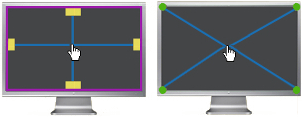
\includegraphics[width=\linewidth]{images/illustrations/prime_pixels}
	\caption{Illustration af kanter, hjørner og museposition hvor "prime pixels" befinder sig, samt linjer der viser den hurtigste lige vej til disse}
	\label{fig:primepixels}
\end{wrapfigure}

Inden for menneske-datamaskine interaktion er Fitts' lov udbredt som optimerings- og forbedringsværktøj ved design af brugergrænseflader. Loven bruges til at udregne tiden det tager at flytte markøren til et element, ud fra elementets størrelse og afstanden til det. Som noteret i \cite{karafillis2012}, kan Fitts' lov bruges som en retningslinje når man designer brugergrænseflader - f.eks. ved at finde størrelser og placeringer af knapper. Det er i den forbindelse vigtigt at have kendskab til "prime pixels", som er de pixels, der ligger i kanten og hjørnerne af skærmen. De kan tilgås ved at flytte markøren til skærmens kant, hvor markøren automatisk stopper, hvilket ses på figur \ref{fig:primepixels}. Derudover er markørens nuværende position også en "prime pixel", som for eksempel kan tilgås ved at højreklikke med musen. Den nemme tilgængelighed af disse pixels gør, at de ofte bliver integreret som centrale dele af brugergrænsefladedesign. Eksempler på dette ses overalt i interaktionen med moderne styresystemer, hvor størstedelen af dem benytter sig af markørens nuværende position til at vise en menu, hvis brugeren højreklikker. Der er også en tendens til at styresystemers proceslinje bliver lagt langs øvre eller nedre kant af skærmen - igen på grund af den lette tilgængelighed af disse "prime pixels". Fleksibiliteten af Fitts' lov ses ved den store variation af brugergrænseflader hvor den kan bruges, blandt andet i drop-down menuer, som beskrevet af \cite{accot1997}. Brugen af Fitts' lov i drop-down menuer ses på figur \ref{fig:dropdown}, hvor det illustreres, at der for hvert trin i menuen vil være en pegeopgave, hvor Fitts' lov kan benyttes.\\

\begin{wrapfigure}{l}{.35\linewidth}
	\centering
	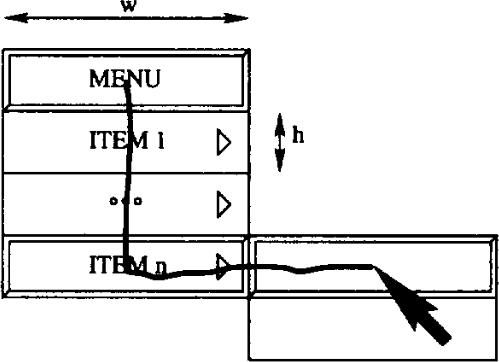
\includegraphics[width=\linewidth]{images/illustrations/dropdown}
	\caption{Illustration af navigation igennem drop-down menu}
	\label{fig:dropdown}
\end{wrapfigure}

Med udviklingen af berøringsfølsomme skærme som primær inputmetode, har der været et behov for at udvikle nye måder at interagere med systemerne på. Tendenserne til at benytte sig af "prime pixels" i brugerfladedesign på styresystemer går igen med berøringsfølsomme skærme. Blandt andet benytter mobilstyresystemerne Android, iOS og Windows Phone sig alle af navigationselementer, som  ligger i kanten af skærmen. Et eksempel på dette ses på figur \ref{fig:notifications}, som viser, hvordan man skal trække fingeren ned fra den øvre kant af skærmen for at tilgå de hurtige indstillinger, og se sine notifikationer. Dette er igen et godt eksempel på brugergrænsefladedesign, hvor der er taget højde for at tiden det tager at interagere med et element på skærmen skal være så kort som overhovedet muligt - især med de elementer, der bruges oftest. Ved disse berøringsfølsomme skærme, vil der være behov for at optimere brugergrænsefladerne, så enhederne er hurtige at benytte sig af.\\

Selvom der kunne være en fordel i at benytte sig af Fitts' lov på berøringsfølsomme skærme, er der stadig behov for mere dokumentation for, at denne rent faktisk kan benyttes til touch-input. Der er dog i løbet af de sidste to år publiceret et antal artikler om Fitts' Lov, hvor forskere er begyndt at se på, om den også kan bruges til berøringsfølsomme skærme eller øjenbevægelser \cite{hong2015} \cite{zhao2015} \cite{jiang2014} \cite{greene2014}. Dette danner et generelt billede af, at Fitts' lov stadig er interessant at skrive om, og forske i, i dag - selvom den blev introduceret i 1954.\\

\begin{wrapfigure}{r}{.35\linewidth}
	\centering
	
\includegraphics[width=\linewidth]{images/illustrations/navigation_dragdown}	
	\caption{Illustration af adgang til hurtigindstillinger og notifikationscenter ved at trække ned fra overkanten af den berøringsfølsomme skærm}
	\label{fig:notifications}
\end{wrapfigure}

Siden udgivelsen af Fitts' originale artikel, der beskrev hans forsøg og udledte formel, har flere andre udgivelser foreslået ændringer, som kunne forbedre Fitts' lov. En af de første udgivelser, som ville ændre Fitts' lov var \cite{welford1968}. Alan T. Welford foreslog nogle ændringer til Fitts' lov, ud fra sine observationer af Fitts' indsamlede data. Både Fitts og Welford beskrev formuleringerne ud fra et rent menneskeligt motorisk synspunkt. Men i slutningen af 70'erne begyndte menneske-datamaskine interaktionsforskere at interessere sig for emnet, blandt andet med udgivelsen af \cite{card1978}. Siden da foreslog David E. Meyer af to omgange \cite{meyer1988, meyer1990}, nogle fundamentale ændringer til den bagvedliggende model for Fitts' lov. Dette førte til en variant af Fitts' lov, hvor sværhedsgraden var beskrevet ved kvadratrod i stedet for en logaritmisk funktion. Meyer lavede først en række beregninger på data fra Fitts' forsøg, hvilket viste, at hans formulering passede bedre på den indsamlede data. Herefter lavede han nogle forsøg, hvor testpersonerne lavede simple håndledsbevægelser. Disse viste igen, at den nye variant passede bedre til den indsamlede data.

I 1992 udgav Scott MacKenzie artiklen \cite{mackenzie1992}, hvori han beskrev en ny variant af Fitts' lov. Denne variant udviser samme form som Shannon's Sætning \cite{goldberg2015} og er siden blevet accepteret som den mest udbredte \cite{guiard2011}. MacKenzie udførte beregninger på data fra allerede udførte forsøg og viste, at hans formulering ville passe bedre på de tidligere indsamlede data. På trods af, at MacKenzie viste, at hans formulering passede bedre på data fra tidligere forsøg, har \cite{drewes2010} vist, at alle fire formuleringer ikke nødvendigvis passer til alle tilfælde af en opgaves sværhedsgrad. Dog noterer \cite{goldberg2015}, at MacKenzie's formulering generelt var bedst at bruge ved opgaver med både lave og høje sværhedsgrader.

På trods af, at MacKenzie's variant er den mest udbredte, står det ofte forskere frit for at bruge den variant de finder bedst passende \cite{drewes2010}. Der bliver i forskellige artikler gjort brug af den variant af Fitts' lov, som passer den indsamlede data bedst. Dette fører til, at forskere skal retfærdiggøre deres valg af Fitts' lov, frem for at bruge tiden på deres egentlige forskningsområde \cite{drewes2010}. Der er behov for en standardmodel af Fitts' lov, da det vil gøre det nemmere for både forskere, undervisere og studerende inden for menneske-datamaskine interaktion.\newpage

Det er generelt, inden for videnskabelige felter, vigtigt at reproducere og dokumentere tidligere udførte forsøg. Dette hjælper med at se om et resultat kan genfindes og beskrive situationer, hvor dette ikke er tilfældet. Det hjælper også med at fjerne undersøgelser, hvor resultaterne ikke kan valideres både under samme og ændrede forhold \cite{hornbaek2014}. Det har inden for menneske-datamaskine interaktion i høj grad været normalt ikke at genskabe forsøg. \cite{hornbaek2014} beskriver at kun $3\%$ af 891 artikler fra forskellige publikationer reproducerer tidligere eksperimenter. Denne mangel på reproducering af forsøg, er især relevant ved større opdagelser inden for menneske-datamaskine interaktion, hvilket Fitts' lov i høj grad kan siges at være.

Vi vil i denne rapport udføre to forsøg, hvis formål er at indsamle data til en analyse af bevægelser, for at sammenligne forskellige varianter af Fitts' lov. Vores forsøg vil være en reproducering af forsøg udført af \cite{accot1997, goldberg2015}, og vil bestå af et kontrolleret laboratorieeksperiment, og et ukontrolleret onlineeksperiment. Det kontrollerede laboratorieeksperiment er medtaget for at sikre data af høj kvalitet, ved at sammenligne med data fra vores onlineeksperiment. Vi vil analysere dataene i forhold til de fire allerede omtalte variationer af Fitts' lov. Dertil vil vi analysere bevægelsesbaner, fart og hastighed, for at se om Fitts' lov kan optimeres.\\

\addcontentsline{toc}{section}{Forventninger til læseren}
\section*{Forventninger til læseren}
Der stilles forventinger til læseren om indledende universitetsmatematik, eksempelvis \cite{kolman2008}, indledende statistik- \& sandsynlighedregning, eksempelvis \cite{ditlevsen2011} og \cite{soerensen2003}. Endvidere forventes et indledende kendskab til menneske-datamaskine interaktion, eksempelvis \cite{hartson2012}.

\addcontentsline{toc}{chapter}{Teori}
\chapter*{Teori}
I dette kapitel vil vi kigge nærmere på teorierne bag Fitts' lov. Vi vil først give en opsummering af Fitts' egne tanker, hvorefter vi beskriver tre alternative formuleringer af Fitts' lov.

\addcontentsline{toc}{section}{Fitts' tre eksperimenter}
\section*{Fitts' tre eksperimenter}
Fitts var interesseret i at vise, at informationsteori kunne bruges til at beskrive det menneskelige motoriske system, og udførte derfor en række eksperimenter \cite{fitts1954}. Fitts udførte i alt tre eksperimenter - det første af dem dog med to forskellige pegeredskaber - hvilket gav anledning til data fra fire forskellige motoriske opgaver. Fitts arbejdede med de tre eksperimenter ud fra følgende hypotese, hvor $E$ kontrollerer den gennemsnitlige amplitude og varighed \cite{fitts1954} og $S$ er forsøgspersonen
\begin{quotation}
\textit{If the amplitude and tolerance limits of a task are controlled by E, and S is instructed to work at his maximum rate, then the average time per response will be directly proportional to the minimum average amount of information per response demanded by the particular conditions of amplitude and tolerance. \cite{fitts1954}[s.263]}
\end{quotation}
Vi vil i denne sektion se nærmere på de tre eksperimenter og Fitts' konklusioner.

\addcontentsline{toc}{subsection}{Eksperiment 1}
\subsection*{Eksperiment 1: \textit{Reciprocal Tapping}}
Fitts gjorde i dette eksperiment brug af et pegeredskab, og seks plader af samme længde. De to af pladerne, centerpladerne, var placeret med en forudbestemt afstand imellem sig. Derudover blev én af hver af de sidste fire plader placeret på hver side af centerpladerne.

De to centerplader kunne antage fire forskellige bredder, og de kunne placeres på fire måder - hver med en ny afstand imellem dem. Testpersonen skulle gentagne gange føre pegeredskabet fra den ene centerplade til den anden, med vægt på præcision frem for fart. De omkringliggende pladers formål, var at måle eventuelle fejl. Figur \ref{fig:FittsEx1} viser opstillingen hvor de to stiplede plader er centerpladerne.

Testdeltagerne, 16 højrehåndede mandlige universitetsstuderende, fik 15 sekunder til hver af de 16 opgaver. Opgaverne blev udført i tilfældig rækkefølge, med en pause på 55 sekunder mellem hver af opgaverne. Eksperimentet blev udført med to forskellige pegeredskaber - et lettere i vægt end det andet.

\addcontentsline{toc}{subsection}{Eksperiment 2}
\subsection*{Eksperiment 2: \textit{Disc Transfer}}
I dette eksperiment brugte Fitts to pinde, og otte runde plader. De otte runde plader havde et hul i midten, som kunne antage fire forskellige størrelser - dog havde alle otte plader den samme hulstørrelse, i hver enkel opgave. De to pinde skulle ligesom i eksperiment 1 være placeret med fire forskellige afstande imellem sig. 

Hver af de 16 forsøgsmuligheder blev i tilfældig rækkefølge udført af 16 højrehåndede mandlige universitetsstuderende. Figur \ref{fig:FittsEx2} viser, hvordan eksperimentet blev udført.

\begin{minipage}[c]{\linewidth}
	\begin{minipage}[b]{.45\linewidth}
		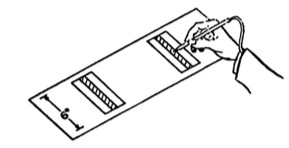
\includegraphics[width=\textwidth]{images/illustrations/fitt_ex1}
		\captionof{figure}{Illustration af Fitts' første eksperiment, med pegeredskab og seks lodrette plader \cite{fitts1954}}
		\label{fig:FittsEx1}
	\end{minipage}
	\begin{minipage}[b]{.1\linewidth}
		~
	\end{minipage}
	\begin{minipage}[b]{.45\linewidth}
		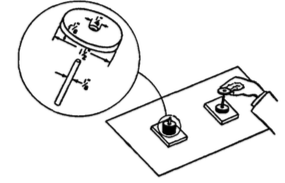
\includegraphics[width=\textwidth]{images/illustrations/fitt_ex2}
		\captionof{figure}{Illustration af Fitts' andet eksperiment med to pinde og otte runde plader \cite{fitts1954}}
		\label{fig:FittsEx2}
	\end{minipage}
\end{minipage}

\addcontentsline{toc}{subsection}{Eksperiment 3}
\subsection*{Eksperiment 3: \textit{Pin Transfer}}
Udførelsen af dette eksperiment krævede et sæt af otte pinde og 16 huller, delt i to sæt. Diameteren på de otte pinde kunne antage fire forskellige størrelser, mens afstanden imellem de to sæt huller kunne være af fem forskellige længder. Opstillingen kan ses i figur \ref{fig:FittsEx3}.
Hver af de 20 mulige forsøgsopstillinger blev udført i tilfældig rækkefølge af 20 mandlige universitetsstuderende.
\begin{figure}[h]
\centering
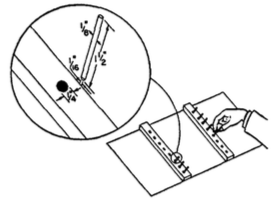
\includegraphics[width=0.5\linewidth]{images/illustrations/fitt_ex3}
\captionof{figure}{Illustration af Fitts' tredje eksperiment med 8 pinde og 16 huller \cite{fitts1954}}
\label{fig:FittsEx3}
\end{figure}

\addcontentsline{toc}{subsection}{Fitts' konklusion}
\subsection*{Fitts' konklusion}
Resultaterne som Fitts fik fra de udførte eksperimenter viste, at des større afstand målene imellem, desto længere tid brugte testdeltagerne. For at bevise sin teori udledte Fitts et \textit{Index of Difficulty} $(ID)$, som beskriver sværhedsgraden af en given motorisk opgave på baggrund af størrelsen, $W$, og afstanden, $A$, til målet.
\begin{align*}
ID = -\log_2\left(\frac{W}{2A}\right)
\end{align*}
Brugen af $\log_2$ i formlen, er baseret på Fitts' kendskab til Shannon's sætning 17 \cite{goldberg2015}. For at sikre, at $ID$ altid giver en positiv værdi, valgte Fitts at gøre brug af $2A$ frem for $A$, da det kan garanteres at $2A > W$, hvilket sikrer det samme fortegn for alle udfald af logaritmen. Da $log\left(\frac{W}{2A}\right)<0$, for $0<\frac{W}{2A}<1$, valgte Fitts at multiplicere det med $-1$, hvilket sikrer at ID altid er positiv.
Ved brug af $ID$ udregnede Fitts et \textit{Index of Performance}, IP, som beskriver, hvordan en opgave er udført i forhold til $ID$, og tiden $t$.
\begin{align*}
IP &= \frac{ID}{t}\Leftrightarrow\\
IP &= \frac{-1}{t}\log_2\left(\frac{W}{2A}\right)
\end{align*}
Denne formel er dog ikke den klassiske formel for Fitts' lov, men ved omregninger kan den findes. Vi ser først på ID.
\begin{align*}
ID &= -\log_2\left(\frac{W}{2A}\right) \Leftrightarrow\\
ID &= -\log_2\left(W\right)-\left(-\log_2\left(2A\right)\right) \Leftrightarrow\\
ID &= \log_2\left(2A\right)-\log_2\left(W\right) \Leftrightarrow\\
ID &= \log_2\left(\frac{2A}{W}\right)
\end{align*}
Vi kan indsætte dette i formlen for IP, og isolere et udtryk for tiden $t$.
\begin{align*}
IP &=\frac{-1}{t}\log_2\left(\frac{W}{2A}\right) \Leftrightarrow\\ 
IP &= \frac{1}{t}\log_2\left(\frac{2A}{W}\right) \Leftrightarrow\\ 
t &= \frac{\log_2\left(\frac{2A}{W}\right)}{IP}
\end{align*}
Da det virker uoverskueligt i sådan en formel at dividere med IP, substitueres denne værdi med $IP = \frac{1}{b}$, hvilket giver anledning til en formel som er nemmere at bruge, og forstå.
\begin{align*}
t &= \frac{\log_2\left(\frac{2A}{W}\right)}{\frac{1}{b}} \Leftrightarrow\\ 
t &= b \cdot \log_2\left(\frac{2A}{W}\right)
\end{align*}
Når man regner med det menneskelige motoriske system, skal der medregnes den tid det tager for et menneske at opfatte at en opgave er startet. Fitts fandt frem til dette led, $a$, ved at benytte lineær regression på sine data.
\begin{equation}
\label{eq:FittsLov}
T = a + b \cdot log_2\left(\frac{2A}{W}\right)
\end{equation}
Dette er hvad der i dag kendes som Fitts' lov.

Crossman og Goodeve \cite{crossman1983} forklarer Fitts' lov som en primær underbevægelse fra startpositionen imod målet, hvorefter der forekommer én eller flere korrigerende underbevægelser. En illustration af bevægelsens hastighed over afstand er vist i figur \ref{fig:CrossmanFitt} med en serie af tre underbevægelser, hvoraf den primære underbevægelse begynder i startpositionen med afstand nul.
\begin{figure}[h]
\centering
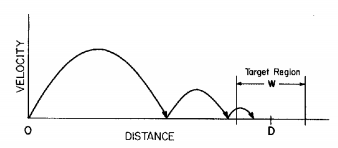
\includegraphics[width=.5\linewidth]{images/illustrations/base_model_fitt}
\caption{Illustration af hastighed over distance, der viser primær og korrigerende underbevægelser brugt af Crossman og Goodeve til at forklare Fitt's lov \cite{meyer1988}}
\label{fig:CrossmanFitt}
\end{figure}

\newpage
\addcontentsline{toc}{section}{Alternative formuleringer}
\section*{Alternative formuleringer}
Siden udgivelsen af Fitts’ artikel, har flere forskere forsøgt at finde en formel, der passer bedre på det motoriske system, end Fitts’ originale lov. Der har inden for menneske-datamaskine interaktion været flere udgivelser, som mener at have fundet en mere korrekt formulering af Fitts’ lov. Vi vil i dette afsnit se nærmere på tre af sådanne formuleringer.

\addcontentsline{toc}{subsection}{Welford's formulering}
\subsection*{Welford's formulering}

I \cite{welford1968} beskriver Welford en række fundamentale forudsætninger for det menneskelige motoriske system. Her kiggede han blandt andet på Fitts' lov, og de data han indsamlede i sit første forsøg. Han mente at Fitts' lov i princippet gengav den indsamlede data præcist, men han så også tre utilfredsstillende egenskaber, hvilket fik ham til at foreslå følgende modifikationer:
Welford argumenterede for, at $A$ ikke skulle multipliceres med $2$, da det på data fra Fitts' første forsøg, ville resultere i en negativ $a$-værdi. Derved bliver (\ref{eq:FittsLov}) til
\begin{align}
\label{eq:Crossman}
T = a + b \cdot \log_2\left(\frac{A}{W}\right)
\end{align}
som også tidligere var blevet udledt af Crossman \cite{crossman1957}. Hvis data fra Fitts' første forsøg indsættes i (\ref{eq:Crossman}), så vil $a$ ligge tæt på $0.05$. Dette passer med Crossman's eksperiment, hvor tiden man bruger, inden bevægelsen begynder, udregnes til at være cirka $0.05$ \cite{crossman1957}. Welford argumenterer for, at man derved helt kunne undlade $a$, da det beskriver tiden inden bevægelsen. I et lignende eksperiment \cite{welford1958} fandt han dog, at resultaterne generelt var mere troværdige, hvis $a$-leddet var medtaget.

Figur \ref{fig:WelfordGraf} viser data fra ét af Fitts' eksperimenter og den tilhørende affine kurve. Den affine kurves skæring med $y$-aksen rammer under nul, jævnfør den negative $a$ værdi. På baggrund af de to første punkter, som ikke ligger på den affine linje, fandt Welford frem til, at følgende modifikationer til (\ref{eq:FittsLov}) ville beskrive datapunkterne bedre.
\begin{align}\label{eq:WelfordsLov}
T = K \cdot \log_2\left(\frac{A + \frac{1}{2}W}{W}\right) = K \cdot \log_2\left(\frac{A}{W} + 0.5\right)
\end{align}
(\ref{eq:WelfordsLov}) er sidenhen blevet kendt som Welfords lov og har betydning for, hvordan tiden, $T$, opfattes. Tiden vil i (\ref{eq:WelfordsLov}) blive afhænging af en Weber Fraction \cite{welford1958}, da testpersonen skal skelne mellem længderne til målets fjerneste og næreste kant. Testpersonen skal altså udvælge en længde, $W$, ud fra den totale længde mellem startpunktet og målets fjerneste kant. Det er her vigtigt at notere, at (\ref{eq:WelfordsLov}) også opretholder den fordel, som Fitts hævdede der var ved at multiplicere $A$ med $2$. Dette ses ud fra det mest ekstreme tilfælde, hvor bevægelsens startpunkt er på målets kant.

I dette tilfælde vil det gælde, at $A = \frac{1}{2}W$, hvorved $T = K \cdot log\left(\frac{A + \frac{1}{2}W}{W}\right) = K \cdot \log_2\left(\frac{W}{W}\right)$. Da $\log_2\left(\frac{W}{W}\right)=\log_2(1) > 0 $ vil $ID$ være positivt.

Den sidste observation, der blev gjort var, at kurven i figur~\ref{fig:WelfordGraf} viser en tydelig udfladning ved lavere værdier af $x$. Welford noterede, at det sandsynligvis var grundet en begrænsende faktor, som beskriver en minimumstid per bevægelse, hvor kort eller uhindret bevægelsen end måtte være. Welford's egne undersøgelser har påvist, at denne begrænsende faktor har betydning for, hvor meget af målet, der rent faktisk bliver brugt. Når målene er brede og længden mellem dem kort, vil testpersonen kun bruge en sub-længde af målets fulde længde. Han overfører mere information end (\ref{eq:WelfordsLov}) ville beskrive, fordi den effektive W er kortere. Den kortere bredde kan i nogen omfang afspejles i en reduktion af fejl og, hvis reduktionen sker med behørigt hensyn, holder (\ref{eq:WelfordsLov}) stadig.

Ud fra de tre ovenstående modifikationer indførte Welford igen Fitts' data fra hans første forsøg i et koordinatsystem. Denne gang havde dataen dog været igennem fejlreduktion og blev sat op imod Welford's formulering, hvilket viste, at (\ref{eq:WelfordsLov}) var bedre til at beskrive dataen end (\ref{eq:FittsLov}). Den affine kurve som Welford kom frem til er at se i figur \ref{fig:WelfordGraf2}.

\begin{figure}[h]
\centering
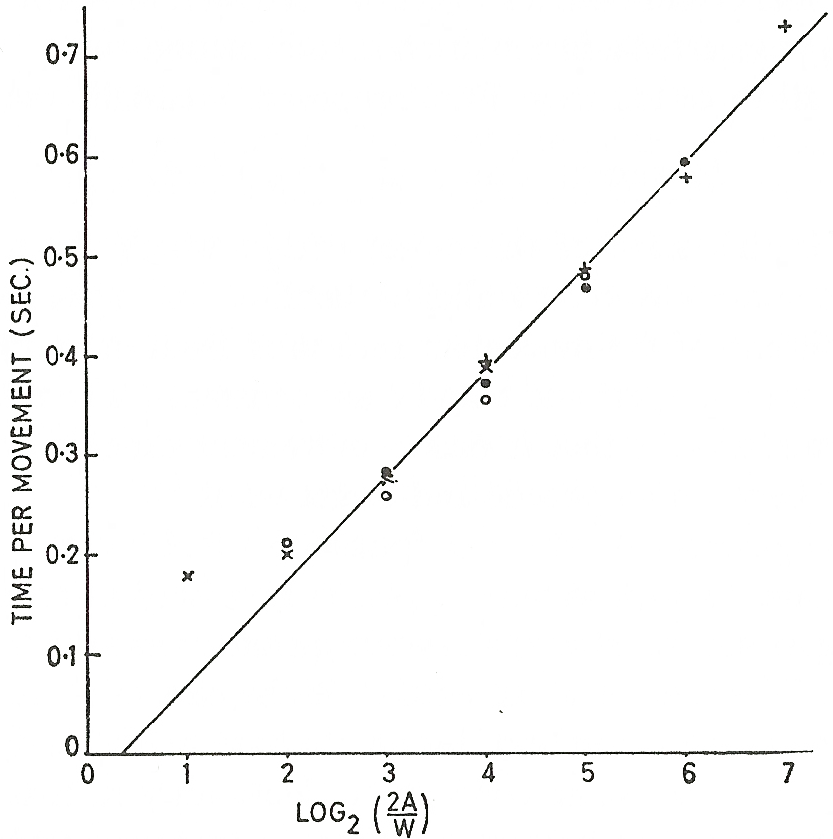
\includegraphics[width=.48\linewidth]{images/illustrations/welford_plot_1}
\caption{Graf over $T$ (y-akse) I forhold til $ID$ (x-akse), med punktplot over data fra et af Fitts' forsøg, og linje der viser hvordan Fitts' model passer på dataene}
\label{fig:WelfordGraf}
\end{figure}

\begin{figure}[h]
\centering
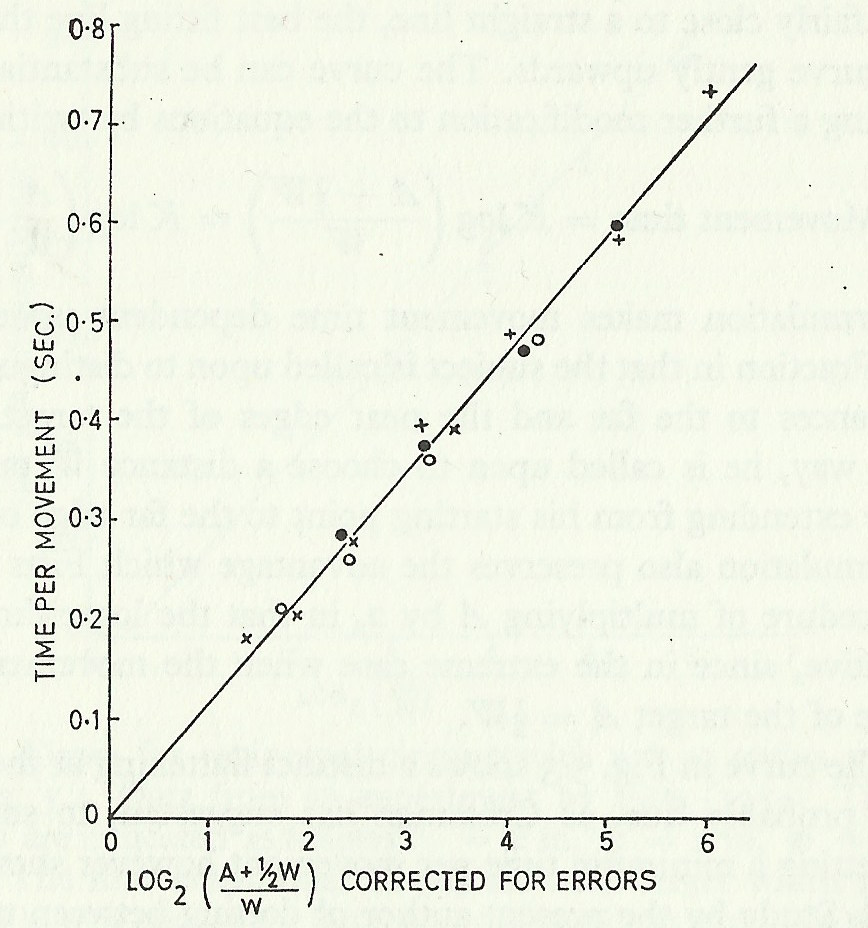
\includegraphics[width=.5\linewidth]{images/illustrations/welford_plot_2}
\caption{Graf over $T$ (y-akse) I forhold til $ID$ (x-akse), med punktplot over data fra et af Fitts' forsøg, og linje der viser hvordan Welford's model passer på dataene}
\label{fig:WelfordGraf2}
\end{figure}

\addcontentsline{toc}{subsection}{MacKenzie's formulering}
\subsection*{MacKenzie's formulering}
MacKenzie udgav i 1992 en artikel~\cite{mackenzie1992}, hvor han ser nærmere på Fitts' lov og seks alternative studier af samme. Han gennemgår en række forbedringer af den originale model, og fremstiller en alternativ formulering til Fitts' lov, som han beskriver som værende mere teoretisk forsvarlig, nemlig:
\begin{align}
T=a+b\cdot\log_2\left({\frac{A+W}{W}}\right)
\end{align}

Han nævner i afsnittet \emph{Physical Interpretation}, at skæringspunktet ideelt set vil ligge i nul, hvilket tyder på, at en opgave med $ID=0$ vil tage 0 sekunder. Ifølge MacKenzie modbevises dette normalt ved lineær regression på forsøgsdata, som ofte medfører et skæringspunkt, der ikke ligger i nul. Dette bruger han som argument for, at der findes en additiv faktor som er urelateret til ID.\\

En af de mest accepterede udledninger af Fitts' lov stammer fra modellen \emph{deterministic error-corrections} originalt fremstillet af \cite{crossman1983}, og bygger på idéen om at en bevægelsesopgave består, af en række iterative korrigerende bevægelser. MacKenzie refererer til simpliciteten af denne model som værende appellerende, men kalder de underliggende antagelser for suspekte. Han refererer til \cite{langolf1976}, hvor der blev observeret bevægelsesopgaver, som kun indeholdte én korrigerende bevægelse, selvom det generelt forudses, at der vil være flere korrigerende bevægelser ved en vis størrelse af $A/W$.\\

\begin{figure}[h]
\centering
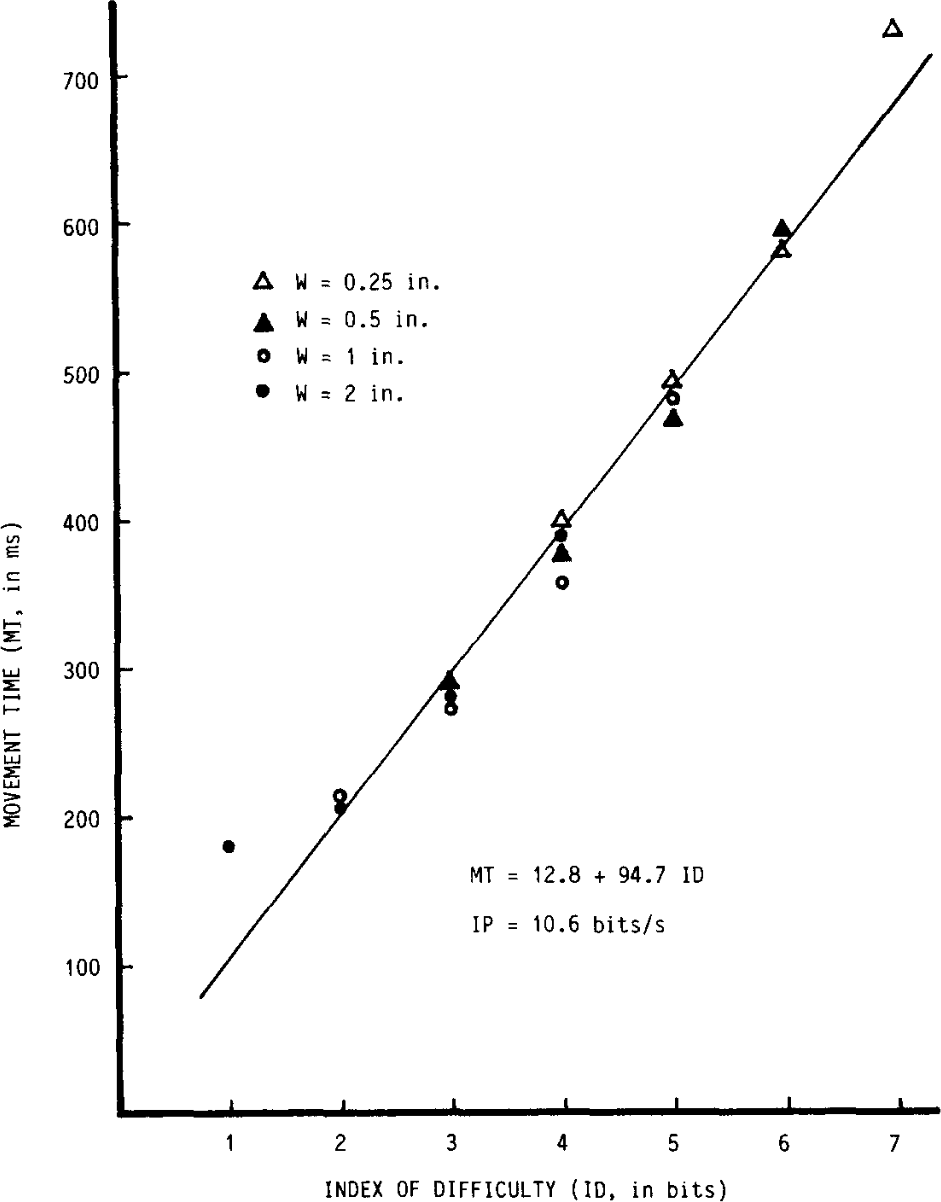
\includegraphics[width=.5\linewidth]{images/illustrations/mackenzie_plot_1}
\caption{Graf over $T$ (y-akse) i forhold til $ID$ (x-akse), med punktplot over data ved forskellige værdier af $W$, og linje der viser hvordan Fitts' model passer på dataen.}
\label{fig:MacKenziePlot1}
\end{figure}
MacKenzie beskriver, at et af problemerne med Fitts' lov er den tætte relation mellem $ID$ og $T$. Figur~\ref{fig:MacKenziePlot1} illustrerer, hvordan punkterne flader ud, ved lave værdier af $ID$, mens kurven beholder sit 1:1-forhold mellem $ID$ og $T$. Der er altså en usammenhæng mellem de observerede og forudsagte værdier, hvilket også er blevet observeret i flere andre studier som \cite{welford1960, buck1986, crossman1983, drury1975, klapp1975, langolf1976, meyer1988, wallace1978}\\
Han fremhæver dog, at der er lavet en del studier af Fitts' lov, og at der er blevet præsenteret en del alternative formuleringer, som forsøger at få de faktiske data til at passe bedre til modellen. Specielt fremhæver han Welford's~\cite{welford1960,welford1968}, da den er udbredt som alternativ til Fitts' originale formulering. MacKenzie nævner den ekstreme lighed mellem Welford og Shannons formulering, og beskriver hvordan det for nyligt er blevet vist at Fitts' originale formulerings forhold mellem $A$ og $W$ havde baggrund i en approksimation af Shannon's sætning~\cite[p. 388]{fitts1954}. Dette mener MacKenzie er et problem, da der i Shannon's sætning er forventning om et højst $S$ til $N$ forhold, imens Fitts gjorde brug af $A$ til $W$ forhold helt ned til 1:1 i sine originale forsøg. MacKenzie foreslår, at man benytter sig af en form der minder meget om Welford's, men er her en direkte analogi til Shannon's formulering:
\begin{align}
\text{Shannon: }C&=b\cdot\log_2{\left(\frac{S+N}{N}\right)}\\
\text{Welford: }T&=a+b\cdot\log_2{\left(\frac{A+0.5W}{W}\right)}\\
\text{MacKenzie: }T&=a+b\cdot\log_2{\left(\frac{A+W}{W}\right)}
\end{align}

Forskellen mellem Fitts' originale formulering og MacKenzie's bud på en ny formulering bliver sammenlignet i figur~\ref{fig:MacKenziePlot2}, hvor det er tydeligt, at der ved lavere værdier af $A$ sker en udfladning af kurven, hvilket passer med datapunkterne i figur~\ref{fig:MacKenziePlot1}, jævnfør det første datapunkt, som ikke ligger på den affine linje.
\begin{figure}[h]
\centering
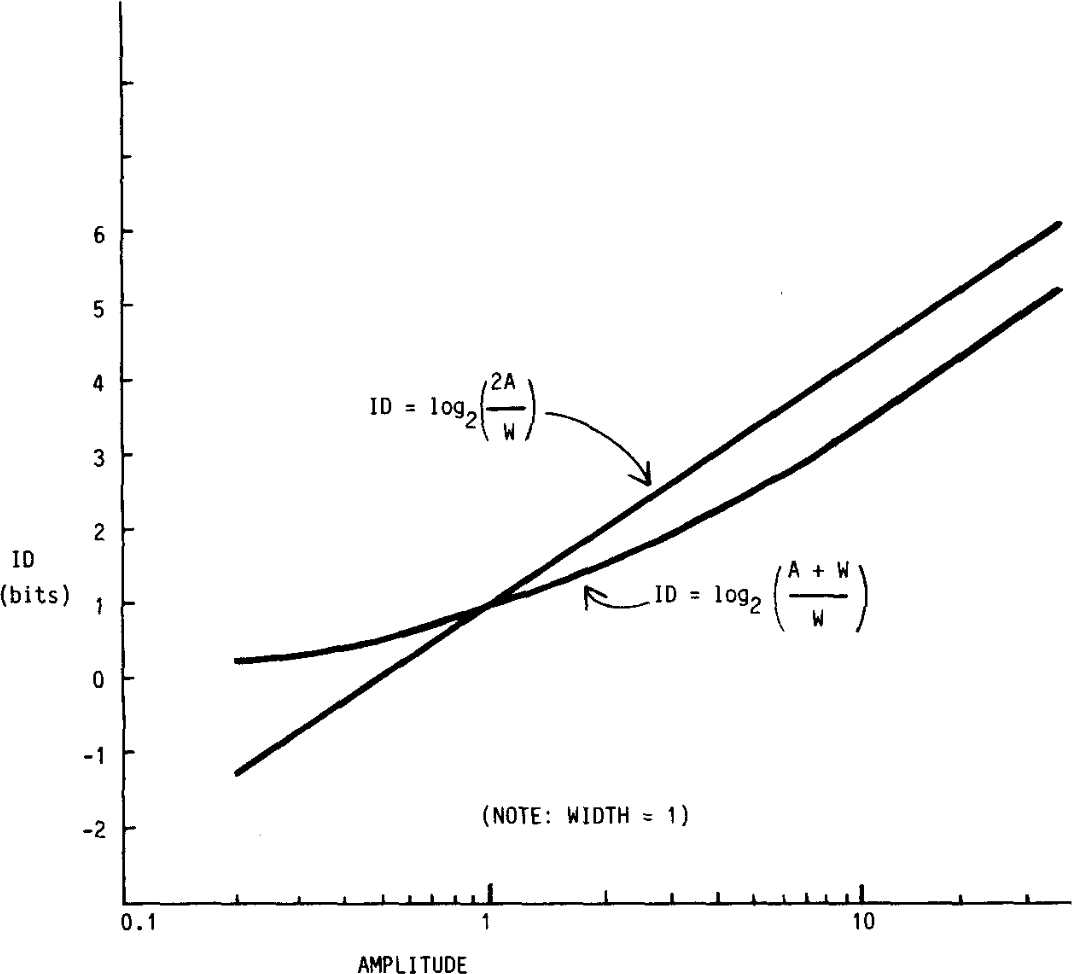
\includegraphics[width=.5\linewidth]{images/illustrations/mackenzie_plot_2}
\caption{Graf over $ID$ (y-akse) i forhold til $A$ (x-akse), med to linjer der viser en sammenligning af Fitts' og MacKenzies model ved fastholdt værdi af $W$}
\label{fig:MacKenziePlot2}
\end{figure}

MacKenzie ser sin formulering som værende en mindre forbedring i forhold til Welford's, og mener ikke, at man vil kunne se den store forskel mellem Welford's og hans egen formulering, medmindre man har at gøre med $ID$ som er under tre bits. Han kommer frem til de tre bits ved at se på figur~\ref{fig:MacKenziePlot2}, hvor, at de to formuleringer for $ID$ er parallelle med hinanden, indtil omkring tre bits eller derunder.

Det generelle problem med MacKenzie's artikel er, at han ikke kommer med noget teoretisk grundlag for sin formulering, og derved ikke kan forklare hvorfor hans formulering er mere præcis end andres, eller hvorfor det netop er bedre med en direkte analogi til Shannon's i forhold til Welford's. I artiklen~\cite{drewes2010} bliver der stillet spørgsmålstegn ved dette. Men hvis man ser bort fra det manglende teoretiske grundlag, er MacKenzies formulering stadig en af de mest udbredte og brugte varianter af Fitts' lov, og har vist sig at passe godt på udførte forsøg~\cite{goldberg2015}.

\addcontentsline{toc}{subsection}{Meyer's formulering}
\subsection*{Meyer's formulering}
Som beskrevet i forrige afsnit, baserer Fitts' lov sig på \emph{deterministic error-corrections} modellen. Meyer et al. foreslog en ny model, kaldet \textit{stochastic optimized-submovement} modellen, som de baserede deres formel på \cite{meyer1988}. Som det ses af figur \ref{fig:MeyerTheory}, baserer denne model sig på, at personer laver én primær underbevægelse og derefter, hvis der er behov for det, én korrigerende underbevægelse. Ud fra denne model kan den gennemsnitlige tid, $T$, forudsiges til at være
\begin{equation}
\label{eq:meyer}
T = a + b \sqrt{\frac{A}{W}}
\end{equation}

\begin{figure}[h]
\centering
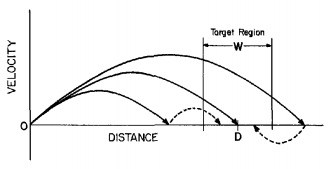
\includegraphics[width=.5\linewidth]{images/illustrations/base_model_meyer}
\caption{\textit{Stochastic optimized-submovement} modellen - Den horisontale akse repræsenterer afstand og den vertikale akse repræsenterer bevægelseshastighed. De faste linjer repræsenterer primære underbevægelser, mens stiplede linjer er korrigerende underbevægelser. Bevægelserne tager udgangspunkt i en startende position (afstand = 0) og skal bevæge sig til et mål, med center i D og bredde W}
\label{fig:MeyerTheory}
\end{figure}

Meyer et al. udfører et teoretisk og to praktiske forsøg. Hvor der i det teoretiske forsøg bliver lavet flere udregninger med forskellige værdier af A og W, som viser en god approksimation i forhold til Fitts' formulering. De praktiske forsøg gør brug af simplere motoriske opgaver end dem kendt fra Fitts' egne forsøg. Den eneste rummelige frihed i Meyers forsøg er håndledets rotation. Igennem hele artiklen benytter Meyer sig af, at en motorisk opgave er delt ind i én primær underbevægelse, og én korrigerende underbevægelse. Dette har dog ikke nogen betydning for sammenligningen med Fitts’ formulering, da den totale tid af alle underbevægelser vil approksimere den logaritmiske funktion af A/W, hvilket medfører at Fitts' model også passer med én korrigerende underbevægelse.

Graferne for funktionerne i (\ref{eq:meyer}) og (\ref{eq:FittsLov}) vil udvise samme form. Grunden til dette er, at begge funktioner er monotont voksende, når $\frac{A}{W}$ bliver større. $\sqrt{\frac{A}{W}}$ vokser dog hurtigere end den tilsvarende logaritmiske funktion, hvilket kan ses af figur \ref{fig:log_vs_sqrt}. 

\cite{goldberg2015} noterer dog, at der er nogle ulemper ved denne formel. Hvis testdeltageren når målet i en enkelt bevægelse, vil modellen følge en lineær udvikling i stedet for en eksponentiel udvikling. Dette passer ikke godt med observerede værdier. For en fast positiv værdi af $\frac{A}{W}$ vil Meyers formel gå mod $1$, når antallet af underbevægelser går mod uendelig.

\begin{figure}[h]
\centering
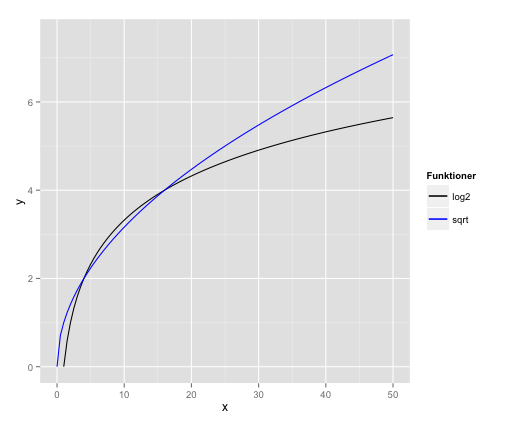
\includegraphics[width=.7\linewidth]{images/illustrations/meyer_plot_comparison}
\caption{Graf over $x$ og $y$ ved et fastdefineret interval, der illustrerer udviklingen af funktionerne $y=log_2(x)$ og $y=sqrt(x)$}
\label{fig:log_vs_sqrt}
\end{figure}

\newpage
\addcontentsline{toc}{section}{Sammenligning}
\section*{Sammenligning}
For at få en bedre forståelse af de fire formuleringer af Fitts' lov, vil vi i dette afsnit se på hvordan de matematisk ligner hinanden. Det første vi vil gøre er, at prøve at omformulere Welford's formulering, da den ikke indeholder et additivt $a$-led. 
\begin{align*}
T &= K\cdot\log_2\left(\frac{A+0.5W}{W}\right)\Leftrightarrow\\
T &= K\left(1-1+\log_2\left(\frac{A+0.5W}{W}\right)\right)\Leftrightarrow\\
T &= -K+K\left(1+\log_2\left(\frac{A+0.5W}{W}\right)\right)\Leftrightarrow\\
T &= -K+K\left(\log_2(2)+\log_2\left(\frac{A+0.5W}{W}\right)\right)\Leftrightarrow\\
T &= -K+K\left(\log_2\left(2\left(\cdot\frac{A+0.5W}{W}\right)\right)\right)\Leftrightarrow\\
T &= -K+K\cdot\log_2\left(\frac{2A+W}{W}\right)
\end{align*}
På trods af, at det er muligt at omskrive Welford's formulering, så vil det ikke være brugbart i praksis. Omformuleringen gør, at $-K$, er negativt, hvilket betyder, at tiden det tager at påbegynde en opgave er negativ. Vi vil derfor fremadrettet kun bruge Welford's formulering uden det additive led.

Da vi har vist, at omskrivningen af Welford's formulering ikke giver logisk mening, vil vi nu kigge på de fire formuleringer, og vise, at de ikke er ens. Dette kan vi gøre ved at vælge en fast værdi for $A$ og $W$, for eksempel, $A = 5$ og $W = 1$. Hvis vi hertil finder ét punkt, hvor formuleringernes funktionsværdier er forskellige, har vi vist, at de ikke er ens. Vi sætter derfor $a=0$ og finder tiden, $T$, til skæringen med $y$-aksen.
\begin{align*}
\text{Fitts: } &T=b\cdot\log_2\left(\frac{2\cdot5}{2}\right)\\
\text{Welford: } &T=k\cdot\log_2\left(\frac{5+0.5\cdot 2}{2}\right)\\
\text{MacKenzie: } &T=b\cdot\log_2\left(\frac{5 + 2}{2}\right)\\
\text{Meyer: } &T=b\cdot\sqrt{\frac{5}{2}}
\end{align*}
Ved at sætte to af ligningerne for $T$ lig hinanden kan vi vise, at de to formuleringer ikke er ens.
\begin{align*}
b_{Fit}\cdot\log_2\left(\frac{2\cdot_25}{2}\right)&=b_{Mac}\cdot\log_2\left(\frac{5 + 2}{2}\right)\\
b_{Mac} &= \frac{b_{Fit}\cdot\log_2\left(\frac{2\cdot5}{2}\right)}{\log_2\left(\frac{5 + 2}{2}\right)}
\end{align*}
Indsætter vi denne værdi for $b_{Mac}$ i MacKenzie's formulering, kan vi finde frem til, at MacKenzie's og Fitts' formuleringer kun er ens, såfremt $ID$-ledet er ens, hvilket ikke er tilfældet.
\begin{align*}
\text{MacKenzie: } &T =\frac{b_{Fit}\cdot\log_2\left(\frac{2\cdot5}{2}\right)}{\log_2\left(\frac{5 + 2}{2}\right)}\cdot\log_2\left(\frac{5 + 2}{2}\right)\\
\text{MacKenzie: } &T =b_{Fit}\cdot\log_2\left(\frac{2\cdot5}{2}\right)
\end{align*}

Denne sammenligning af formuleringerne to og to kan gøres for dem alle fire, men det vil vi undlade at gøre her, og blot formode, at det rent faktisk er tilfældet for dem alle sammen. De fire formuleringer er derfor ikke ens og vi vil derfor få forskellige resultater når vi bruger dem på den indsamlede data.

På trods af, at de fire formuleringer er forskellige, vil de kunne approksimere hinanden. Vi har derfor plottet de fire formuleringer i et interval, for at se om de approksimerer hinanden. Figur \ref{fig:Sammenligning} viser $ID$ som funktion af $A/W$ og viser at Meyer's, Welford's og MacKenzie's approksimerer hinanden for $A/W$-værdier mellem 0 og 25. Grafen for Fitts' ligger højere end de tre andre og approksimerer ikke de andre.

\begin{figure}[h]
\centering
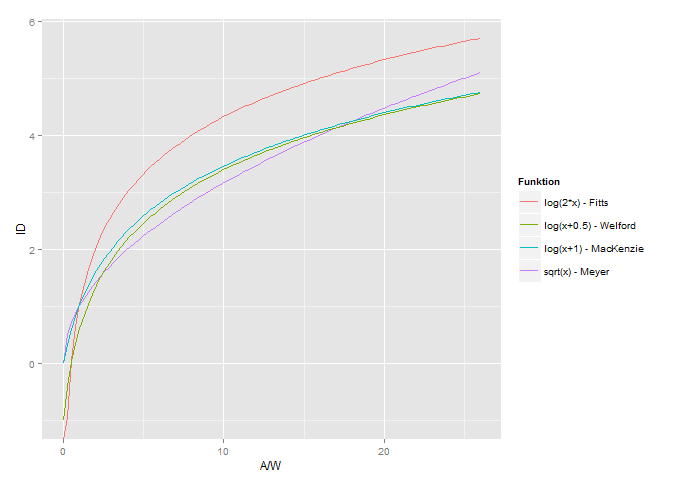
\includegraphics[width=\linewidth]{images/plots/plot_comparison_id}
\caption{Graf over $ID$ (y-akse) i forhold til $A/W$ (x-akse) med linjer, der viser udviklingen af $ID$-funktionen for de fire forskellige modeller}
\label{fig:Sammenligning}
\end{figure}

\addcontentsline{toc}{chapter}{Design}
\chapter*{Design}
I dette afsnit beskriver vi det design, som ligger til grunde for vores forsøg. Dertil vil vi også beskrive vores forsøgsopstillinger.

\addcontentsline{toc}{section}{Forsøgsopstilling}
\section*{Forsøgsopstilling}
Vi har valgt at udføre to brugerundersøgelser, for at have både et kontrolleret og et ukontrolleret datasæt med deltagernes bevægelsesbaner.
Det første vil være et laboratorieeksperiment, hvor vi kontrollerer flest mulige variable, mens det andet er et crowdsourcing- og webbaseret eksperiment, hvor vi får en større mængde data, men ikke har den samme kontrol over eksperimentets variable.\\\\
Vi har valgt at udføre større dele af vores eksperimenter, som tidligere udførte forsøg, da de er udført af eksperter med langt mere erfaring på dette område end os.
Det drejer sig om følgende dele af vores eksperiment:
\begin{itemize}
\item Spørgsmål som blev stillet før crowdsourcing-deltagerne kunne udføre forsøget \cite{goldberg2015}
\item Design af pegeopgave, inklusiv værdier af A, W og canvas\footnote{Den del af skærmen, hvor alle de grafiske elementer bliver tegnet} \cite{goldberg2015}
\item Størrelser af A og W til tunnelopgave \cite{accot1997}
\item Antal vindinger af spiral til spiralopgave \cite{accot1997}
\end{itemize}
Derudover har vi brugt samme udformning af tunnel- og spiralopgave, som i pegeopgaven. Det vil sige, at vi har samme farver til mål, og samme design af testfladen.

\addcontentsline{toc}{section}{Platform og udviklingsværktøj}
\section*{Platform og udviklingsværktøj}
Vi har valgt at bruge JavaScript til at udvikle vores forsøg, da vi alle er bekendte med sproget, så vi skal ikke sætte os ind i noget nyt. Derudover er det integreret i alle browsere nu om dage, hvilket gør det nemt at crowdsource. For at generere vores opgaver har vi valgt at gøre brug af JavaScript-frameworket $paper.js$. Det gør brug af HTML5 Canvas og er bagudkompatibelt til Internet Explorer 9. Frameworket gør det muligt at autogenerere cirkler til vores pegeopgaver, gemme bevægelsesbaner og tegne elementer, til vores tunnel- og spiralopgaver.

\addcontentsline{toc}{section}{Opgavetyper}
\section*{Opgavetyper}
I denne sektion vil vi beskrive, hvordan tunnel-, spiral- og pegeopgaverne er designet. Undervejs i dette afsnit har vi inkluderet visuelle eksempler der er beskåret. I bilag \ref{sec:screenshots} har vi vedlagt figurer, der illustrerer de samme, og flere, eksempler uden nogen beskæring, så canvas, tekst og knapper er med.

\addcontentsline{toc}{subsection}{Tunnelopgave}
\subsection*{Tunnelopgave}
\begin{minipage}{\linewidth}
	\begin{minipage}{\textwidth}
		\centering
		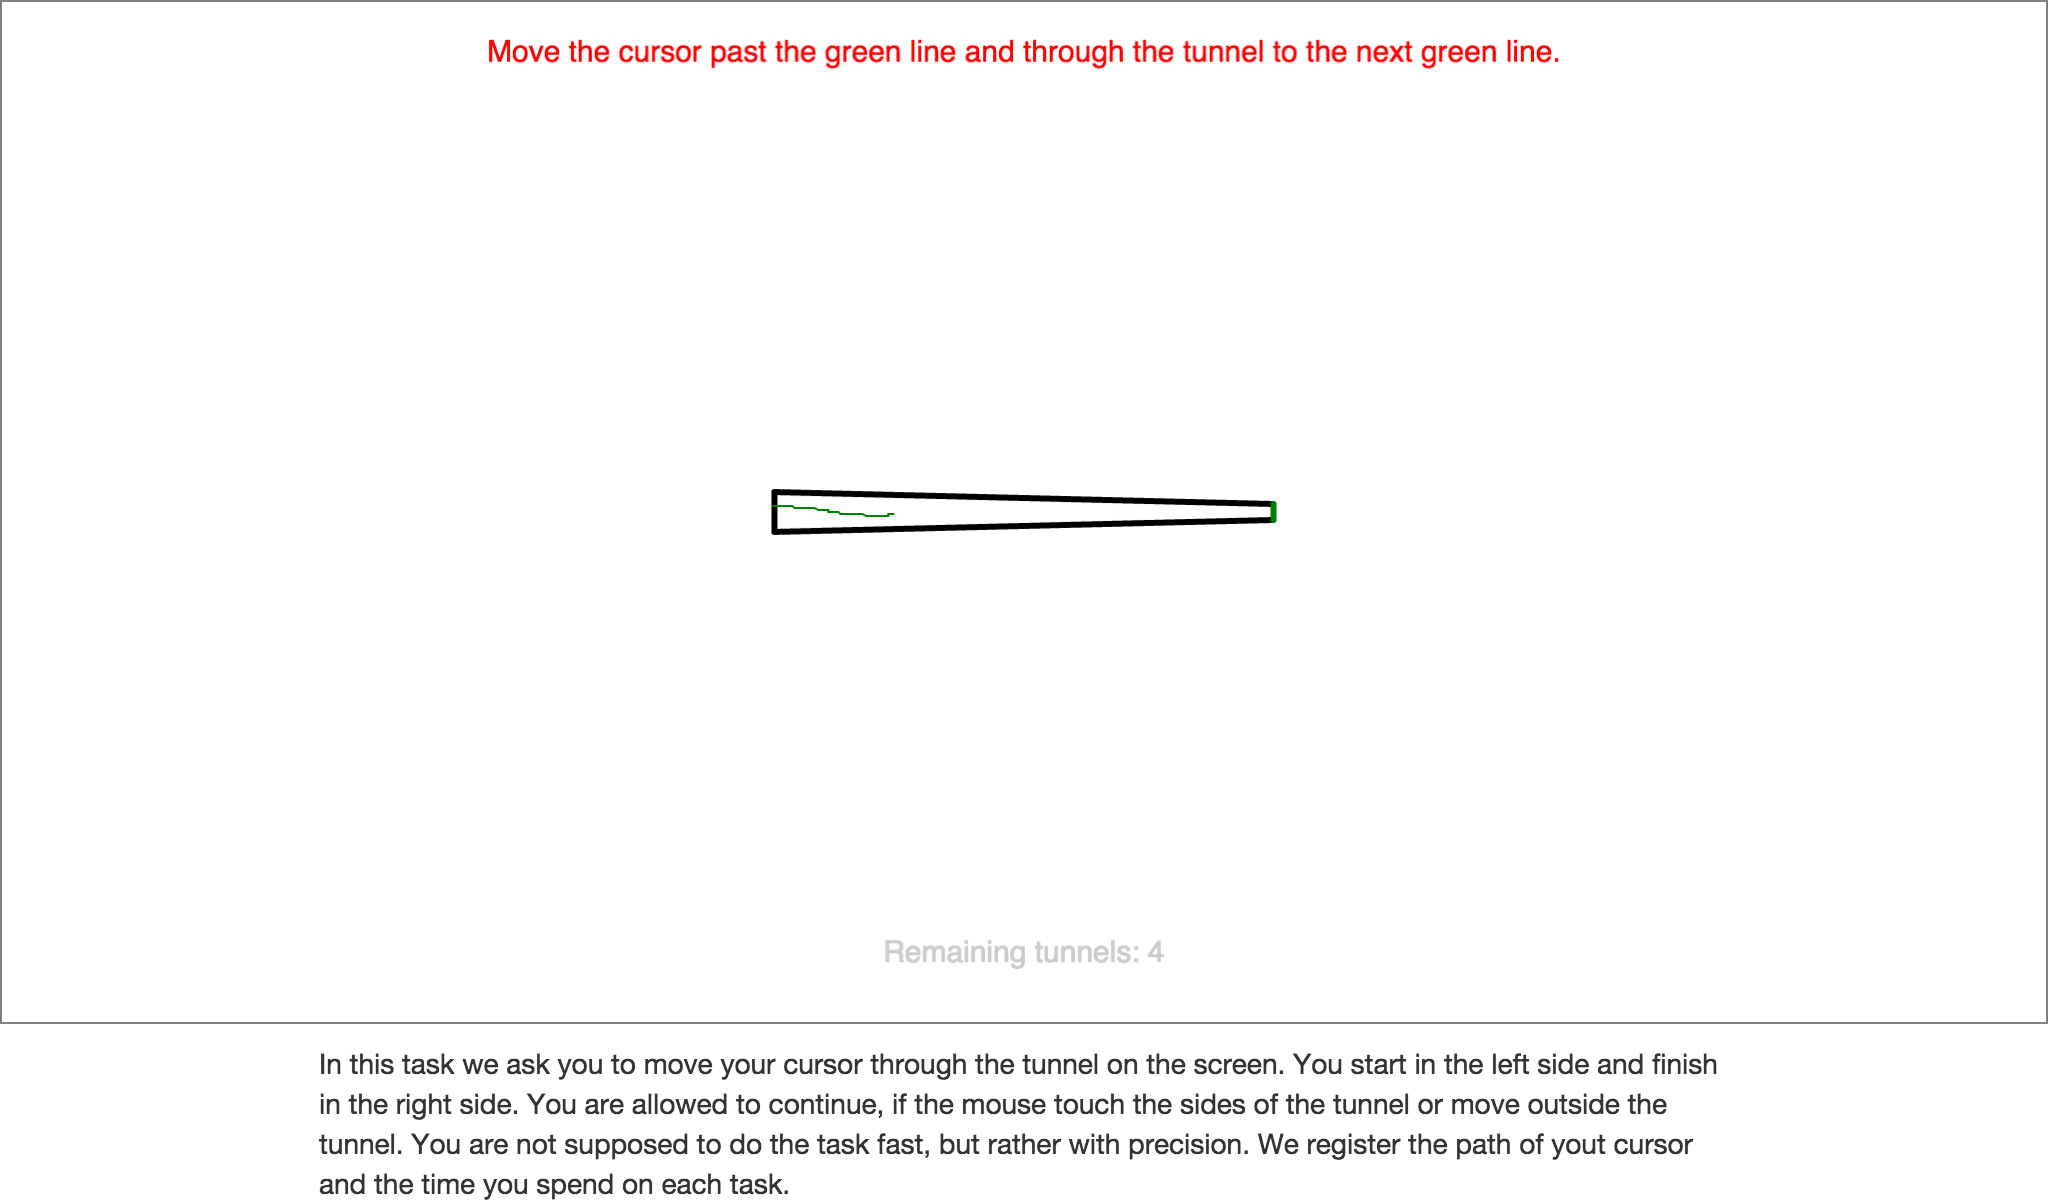
\includegraphics[width=\textwidth, trim = .5cm 23cm .5cm 15cm, clip]{images/screenshots/ex_step_4_tunnel_path}
		\captionof{figure}{Skærmbillede af den første tunnelopgave, med starten af en testpersons sti}
		\label{fig:ex_tunnel_1}
	\end{minipage}
	\begin{minipage}{\textwidth}
		\centering
		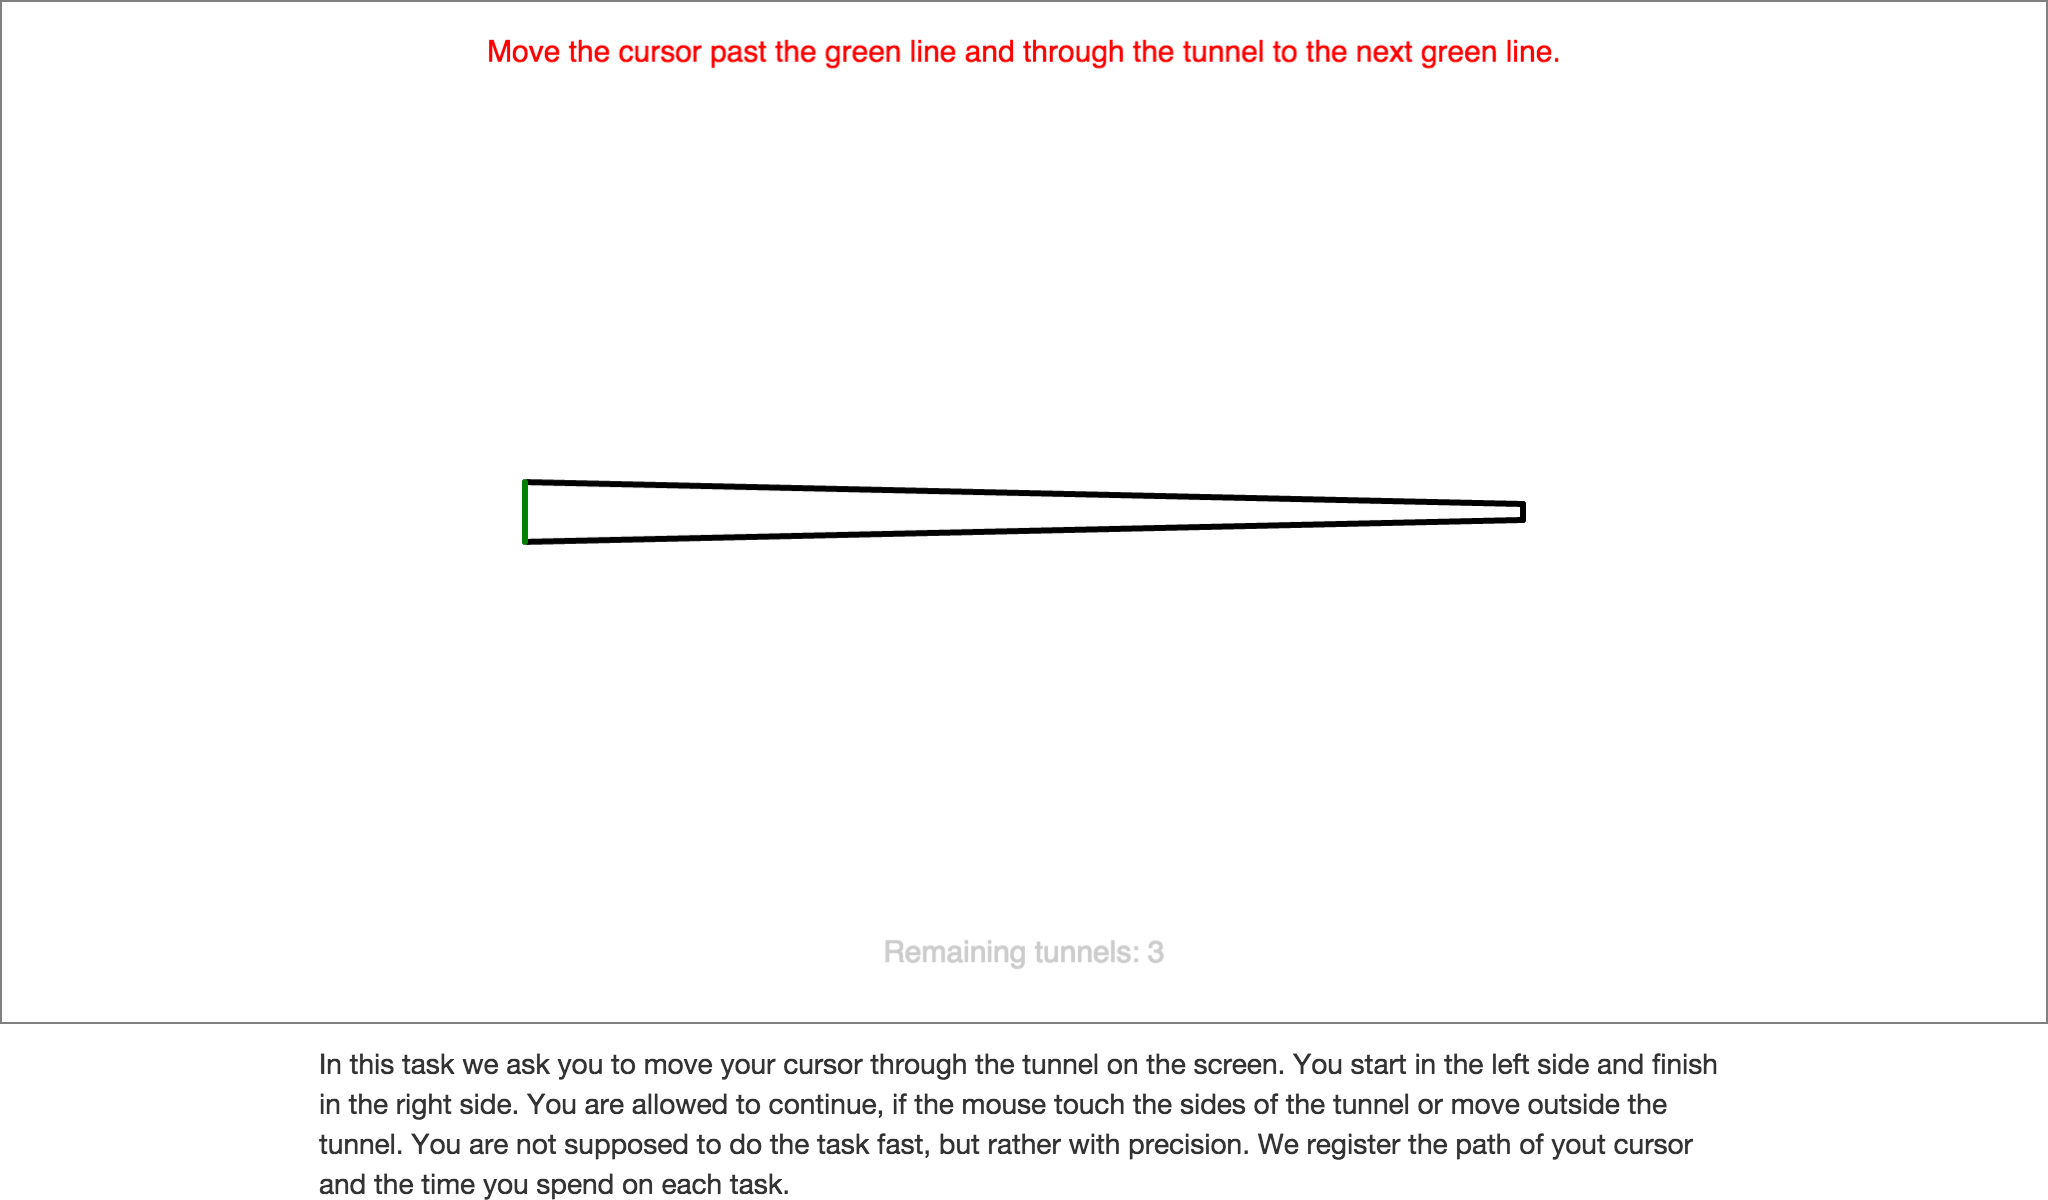
\includegraphics[width=\textwidth, trim = .5cm 22cm .5cm 15cm, clip]{images/screenshots/ex_step_4_tunnel_2}
		\captionof{figure}{skærmbillede af den anden tunnelopgave}
		\label{fig:ex_tunnel_2}
	\end{minipage}
	\begin{minipage}{\textwidth}
		\centering
		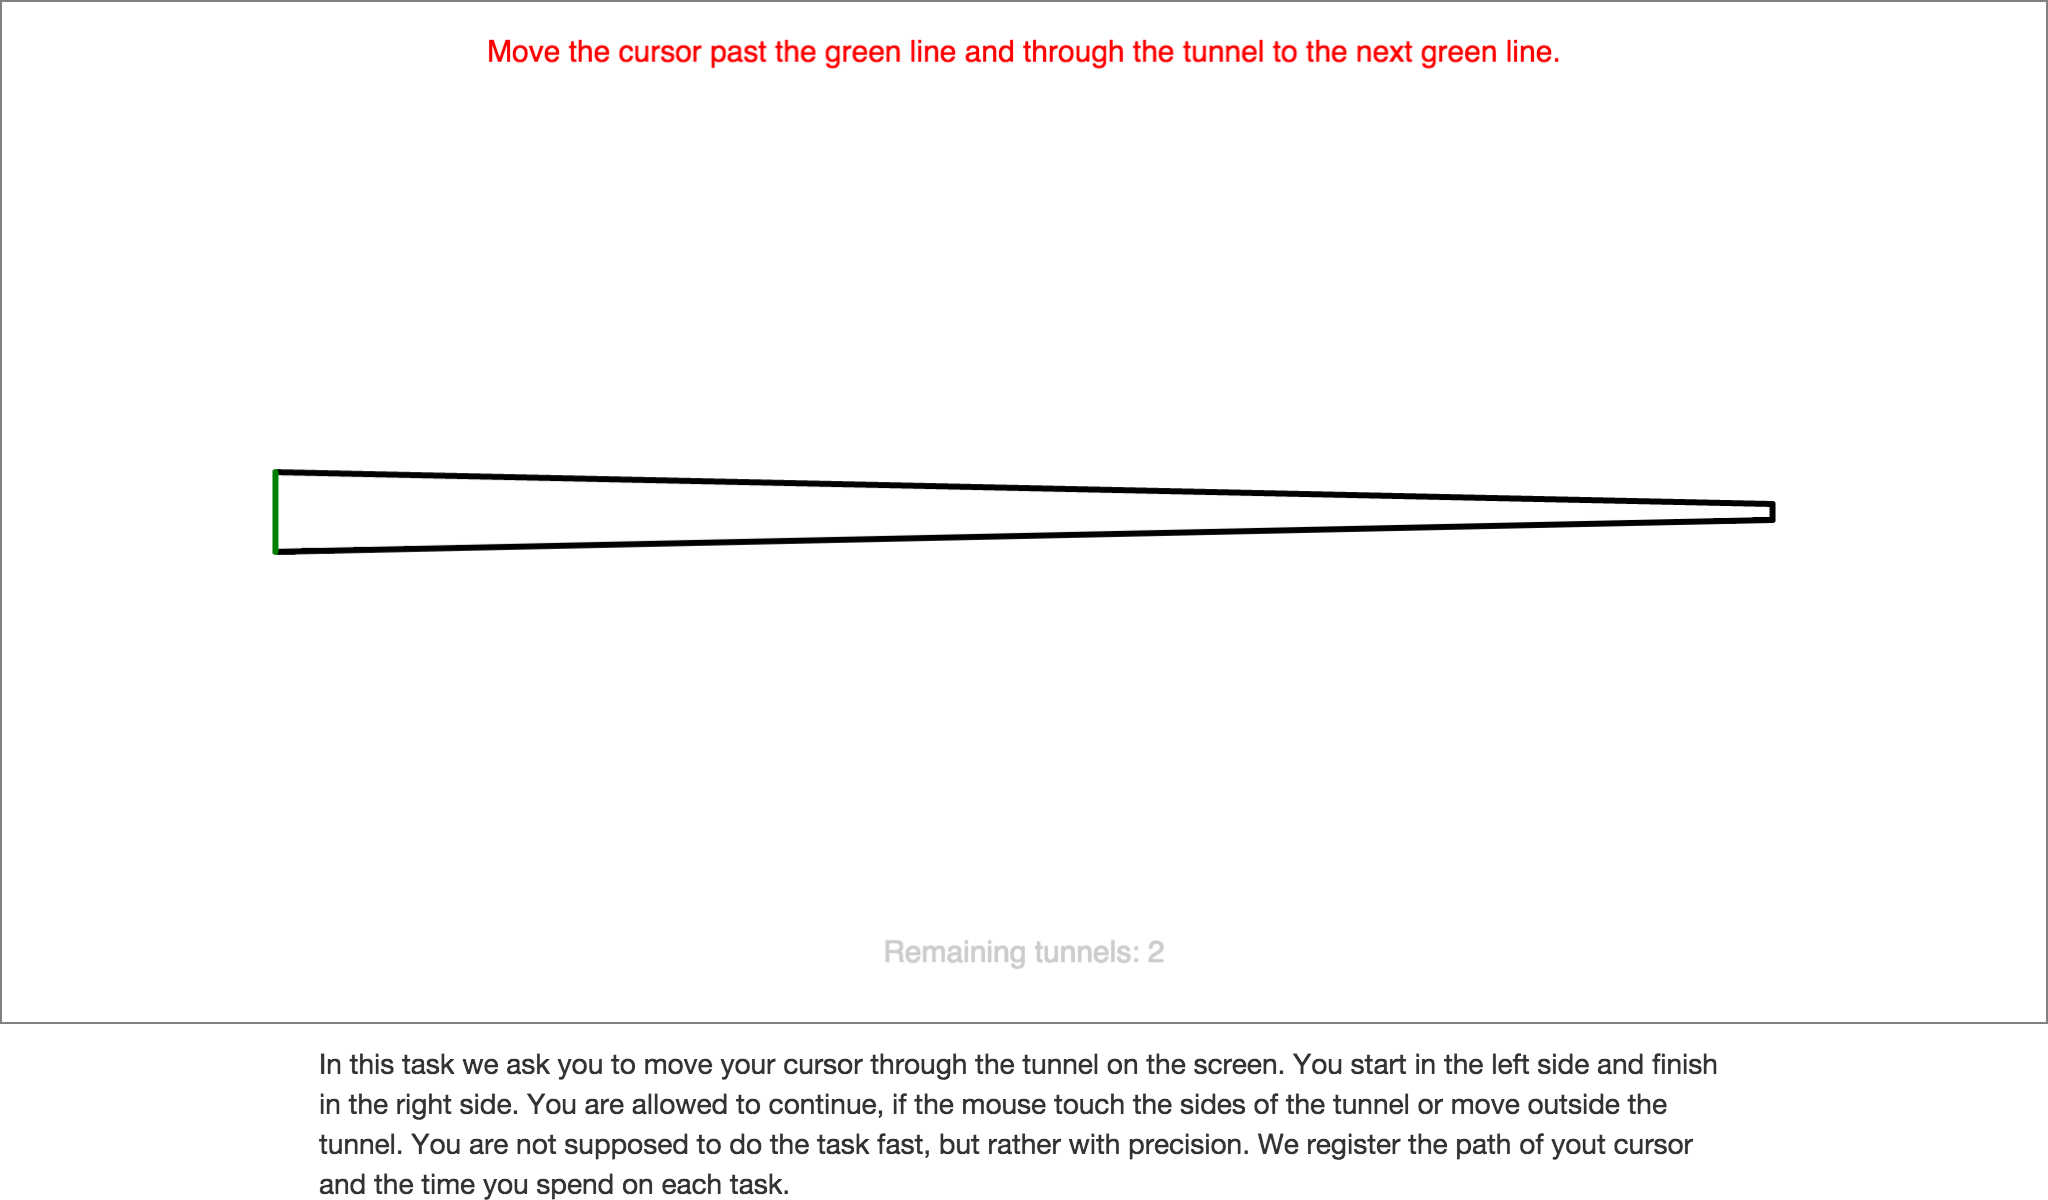
\includegraphics[width=\textwidth, trim = .5cm 21cm .5cm 15cm, clip]{images/screenshots/ex_step_4_tunnel_3}
		\captionof{figure}{Skærmbillede af den tredje tunnelopgave}
		\label{fig:ex_tunnel_3}
	\end{minipage}
	\begin{minipage}{\textwidth}
		\centering
		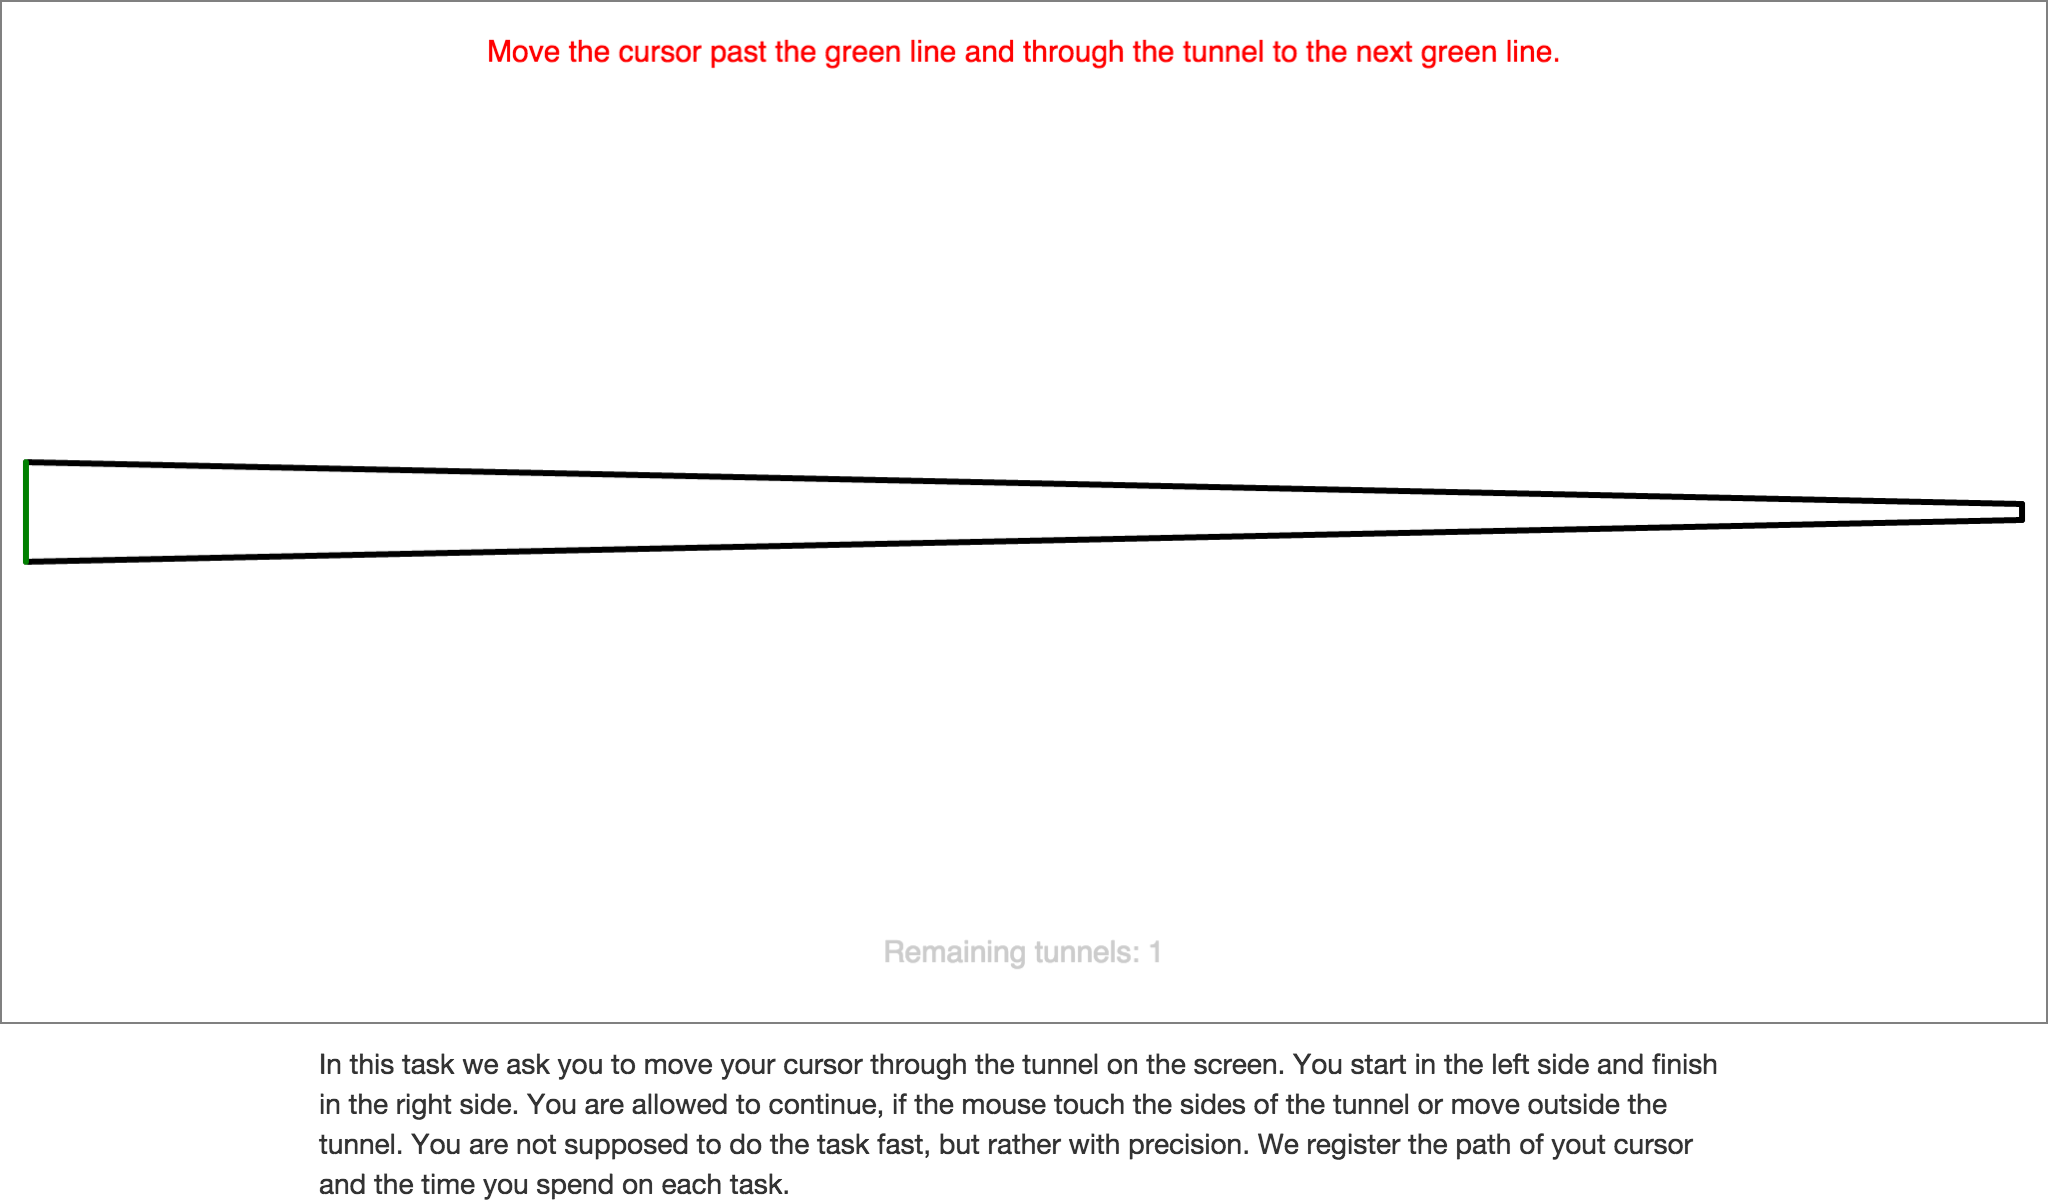
\includegraphics[width=\textwidth, trim = .5cm 20cm .5cm 15cm, clip]{images/screenshots/ex_step_4_tunnel_4}
		\captionof{figure}{Skærmbillede af den fjerde tunnelopgave}
		\label{fig:ex_tunnel_4}
	\end{minipage}
\end{minipage}\\\\
I denne opgave skal testdeltageren føre sin markør igennem fire tunneller af varierende længde, og varierende bredde på startlinjen. De fire tunneller kan ses på Figur \ref{fig:ex_tunnel_1}, \ref{fig:ex_tunnel_2}, \ref{fig:ex_tunnel_3} og \ref{fig:ex_tunnel_4}, hvor de er skaleret ned til 50\% af deres oprindelige forhold, så deres indbyrdes relative størrelse er bevaret.  Størrelserne målt i pixels for tunnellængde, $A$, og den venstre lodrette linje, startlinjen $W_1$, er vist i tabel \ref{tab:tunnelopgave}. Den højre lodrette linje, slutstregen $W_2$, er fastsat til 8 pixels bredde, hvilket stemmer overens med forsøget lavet i \cite{accot1997}
\begin{center}
	\begin{tabular}{c c c c}
		Tunnel & $A$ & $W_1$ & $W_2$ \\
		\hline
		1 & 100 & 20 & 8 \\
		2 & 250 & 30 & 8\\
		3 & 300 & 40 & 8\\
		4 & 400 & 50 & 8\\
	\end{tabular}
	\captionof{table}{Størrelse i pixels af $A$ (længde) og $W$ (startstregen) af tunneller brugt i tunnelopgaverne}
	\label{tab:tunnelopgave}
\end{center}
Ved begyndelsen af en tunnelopgave vil startstregen af tunnellen være markeret med grøn for at tydeliggøre, hvor opgaven starter. Når testdeltagerens markør passerer venstre side af tunnellen vil opgaven starte, og det vil nu være den højre side af tunnellen der er grøn, for at signalere hvor markøren herefter skal flyttes hen. Når opgaven er i gang, vil der som på figur \ref{fig:ex_tunnel_1}, blive vist en grøn linje der hvor markøren flyttes fra. I tilfælde af at testdeltageren rammer eller ryger uden for kanterne, vil de kunne fortsætte ubemærket.

Når testpersonen passerer slutstregen af tunnellen vil opgaven stoppe, og der vil blive vist en knap, hvor testpersonen kan fortsætte til næste opgave, eller afslutte denne test, hvis sidste opgave er gennemført. Ved afslutningen af de fire tunnelopgaver vil tunnellernes længde og bredde, og markørens bane, blive gemt - og til sidst sendt til vores database.

\addcontentsline{toc}{subsection}{Spiralopgave}
\subsection*{Spiralopgave}
\begin{minipage}{\linewidth}
	\centering
	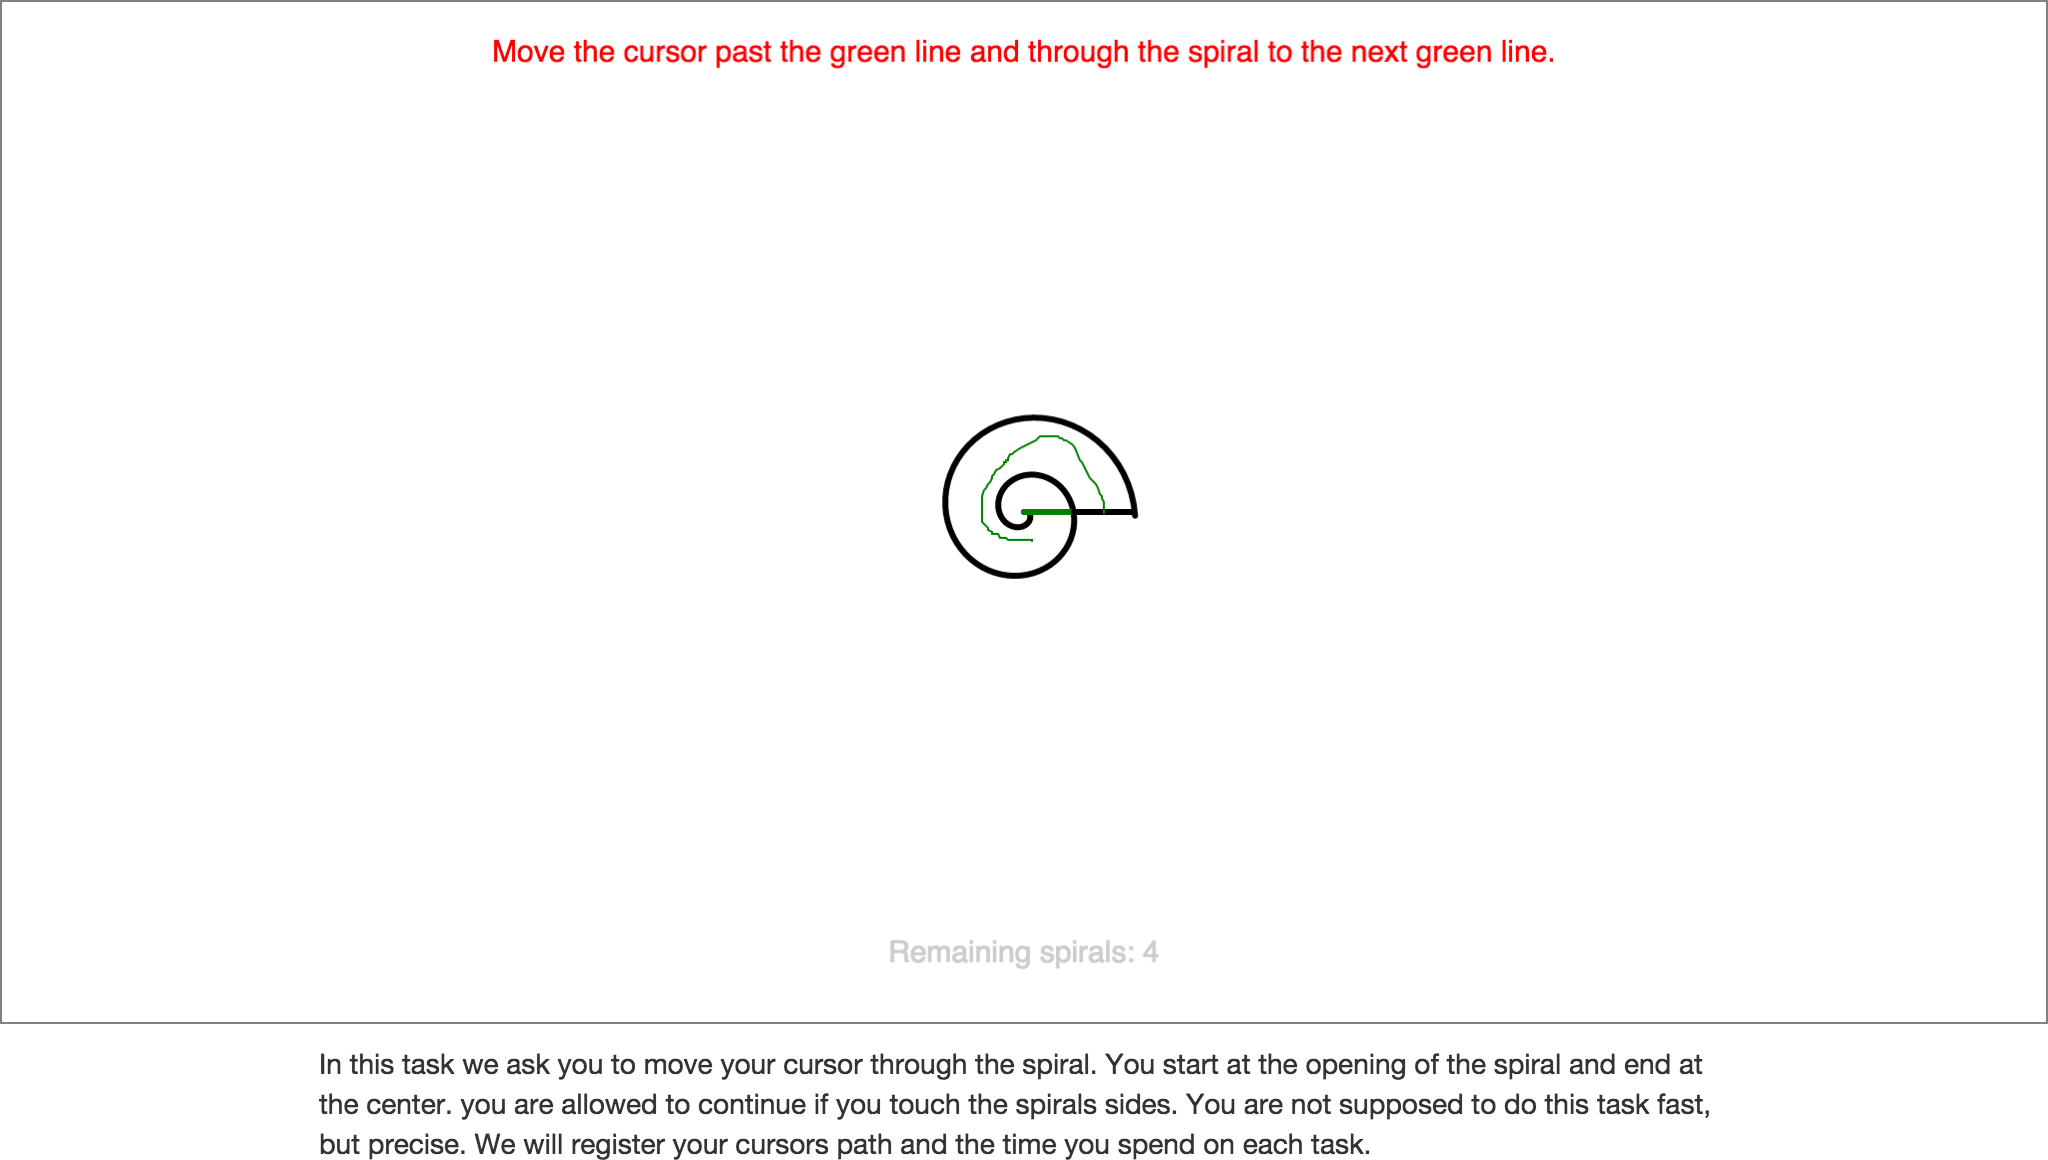
\includegraphics[width=.4\linewidth, trim = 5cm 20cm 5cm 8cm, clip]{images/screenshots/ex_step_5_spiral_path}
	\captionof{figure}{Skærmbillede af den første spiralopgave, med starten af en testpersons sti}
	\label{fig:ex_spiral_1}
	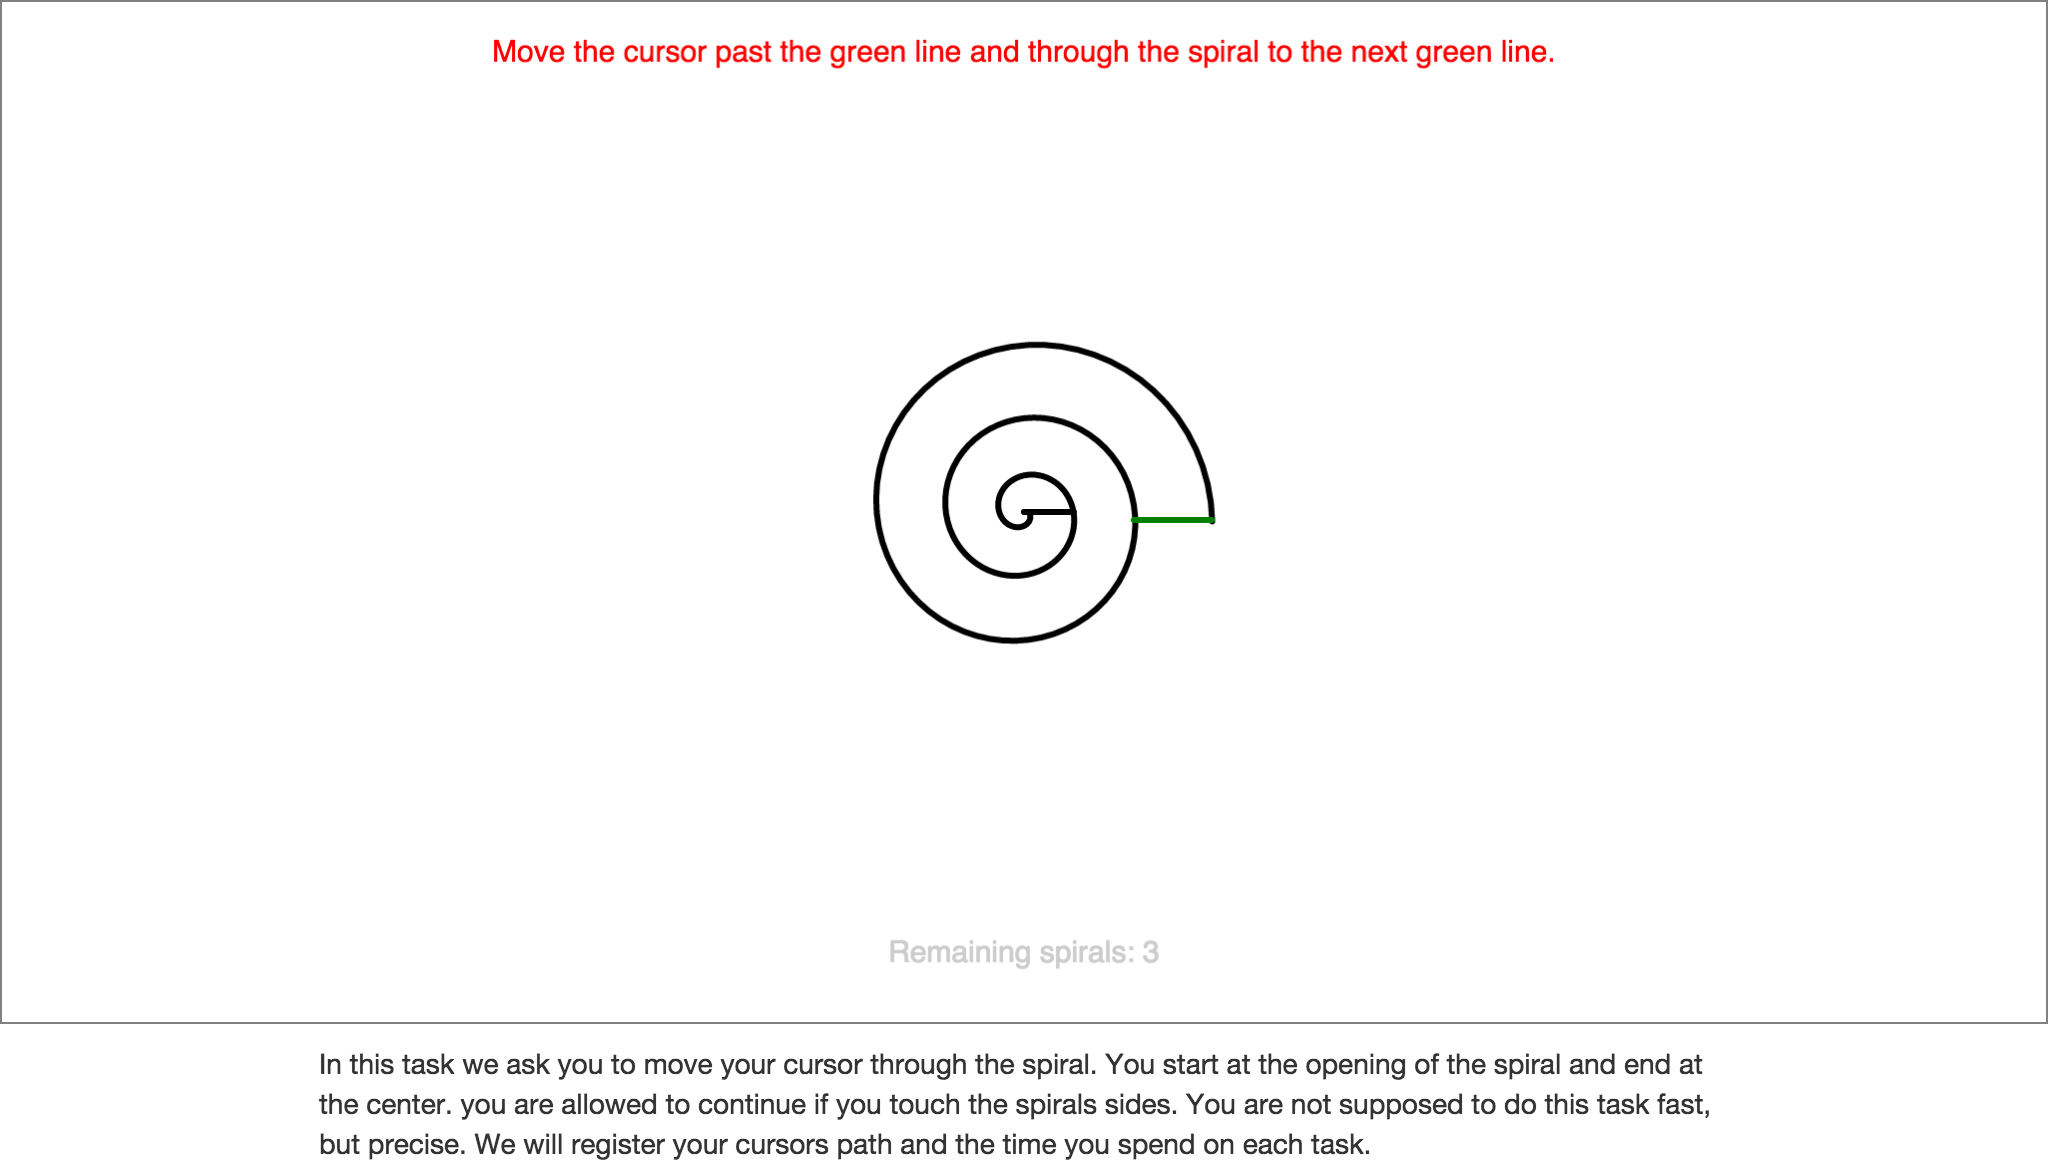
\includegraphics[width=.4\linewidth, trim = 5cm 18.1cm 5cm 8cm, clip]{images/screenshots/ex_step_5_spiral_2}
	\captionof{figure}{Skærmbillede af den anden spiralopgave}
	\label{fig:ex_spiral_2}
	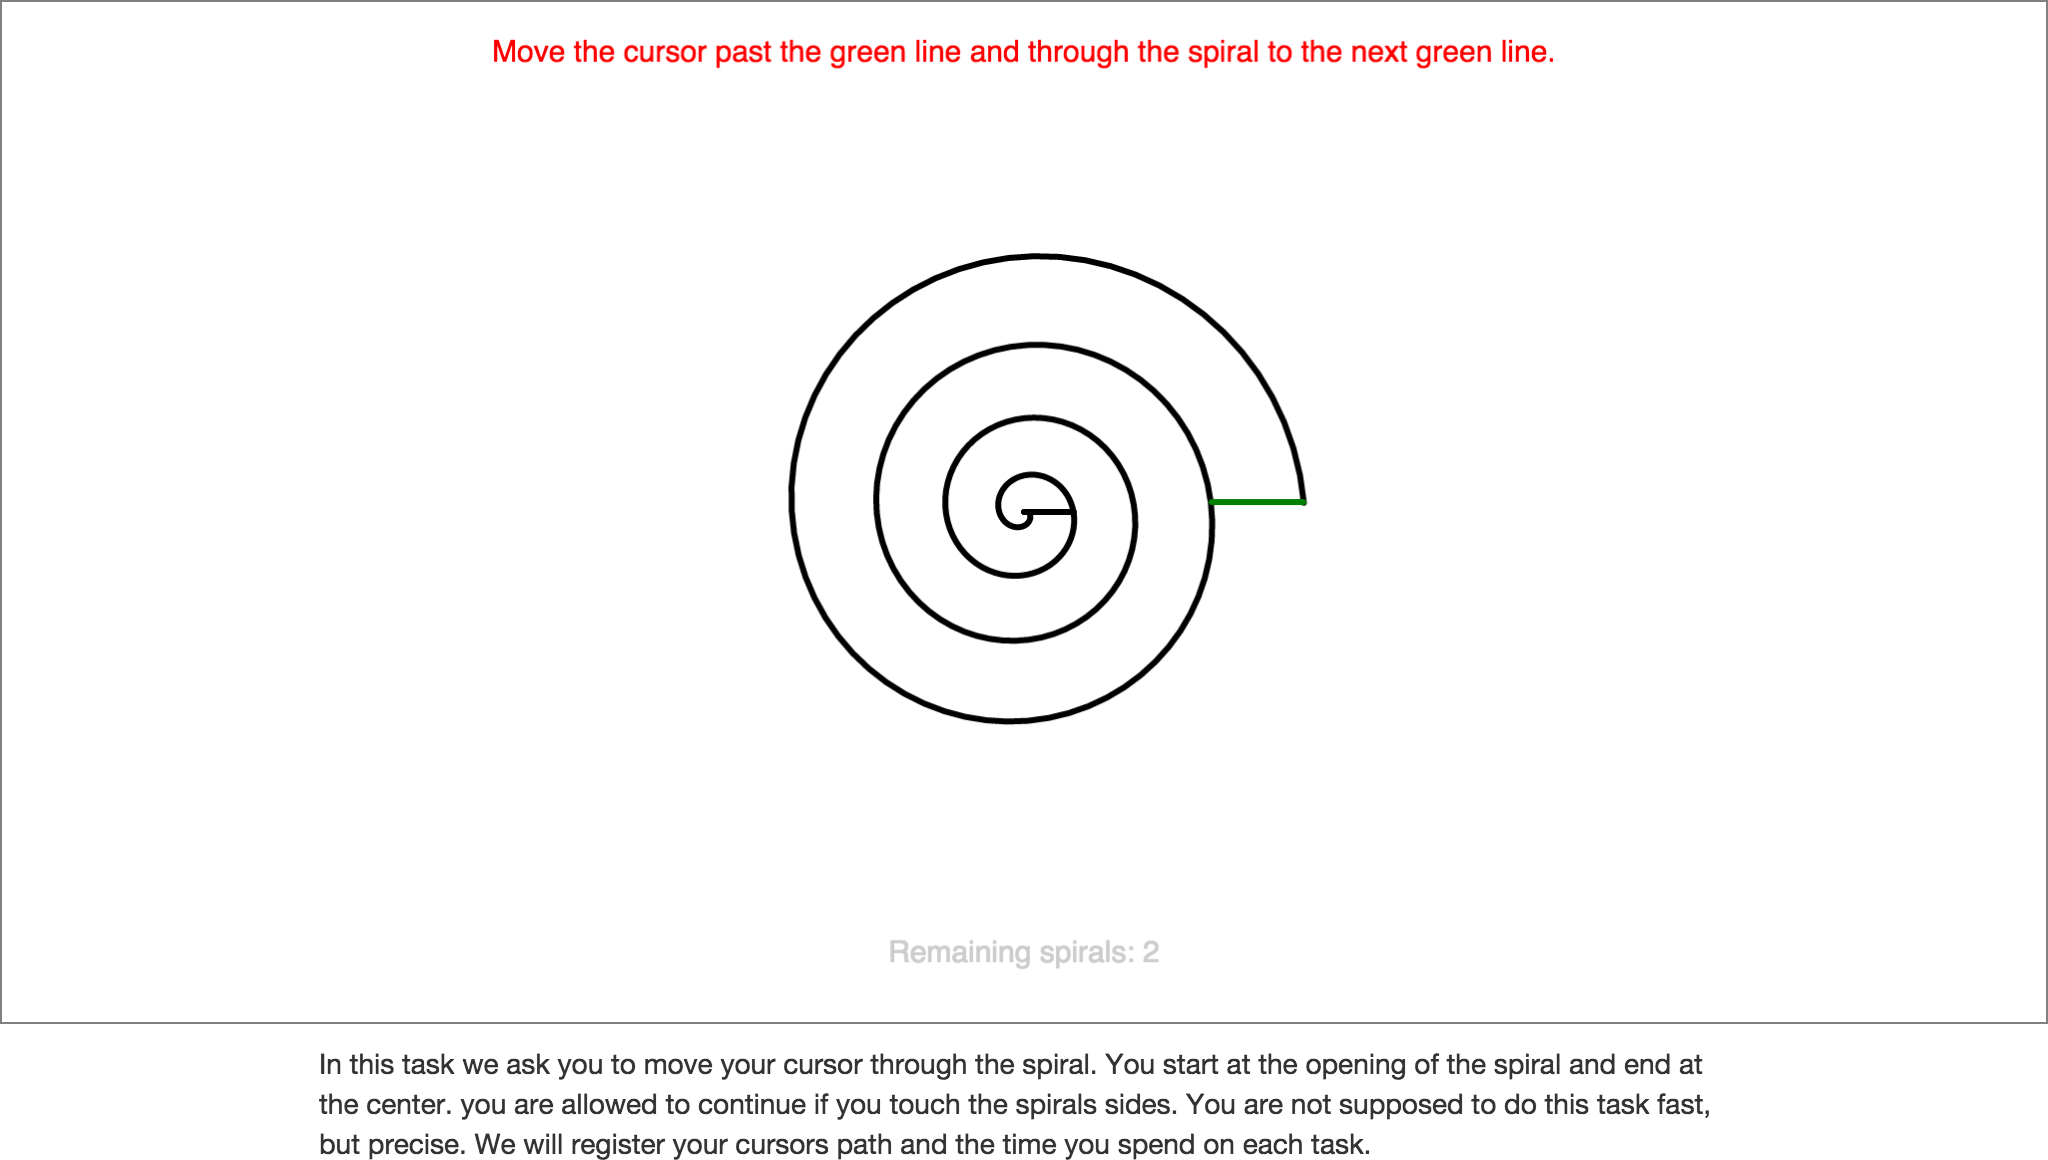
\includegraphics[width=.5\linewidth, trim = 5cm 15.4cm 5cm 8cm, clip]{images/screenshots/ex_step_5_spiral_3}
	\captionof{figure}{Skærmbillede af den tredje spiralopgave}
	\label{fig:ex_spiral_3}
	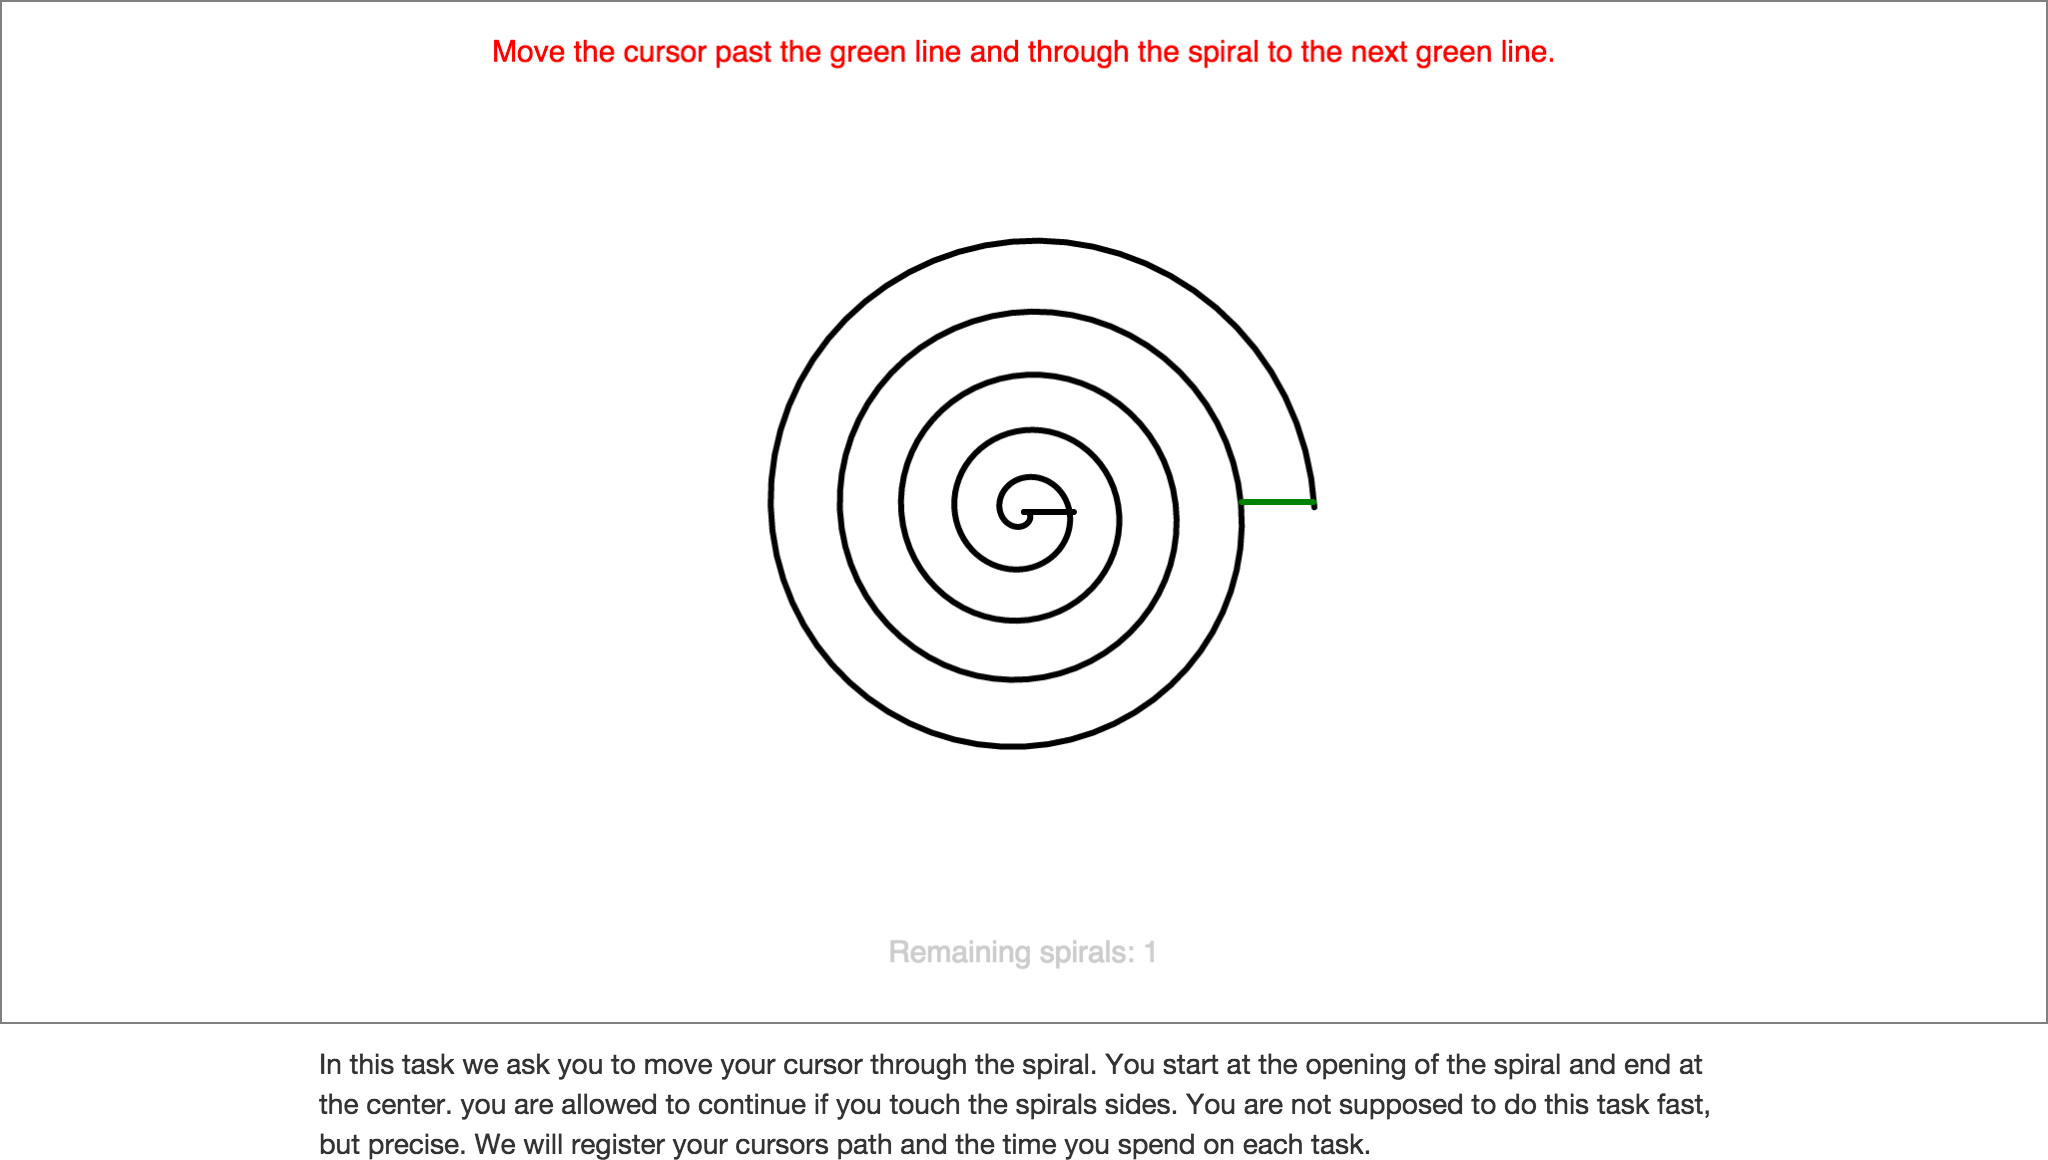
\includegraphics[width=.5\linewidth, trim = 5cm 14.3cm 5cm 8cm, clip]{images/screenshots/ex_step_5_spiral_4}
	\captionof{figure}{Skærmbillede af den fjerde spiralopgave}
	\label{fig:ex_spiral_4}
\end{minipage}\\\\
I denne opgave skal testdeltageren føre sin markør gennem fire spiraler af varierende størrelse, og med varierende antal vindinger. De fire spiraler kan ses på figur \ref{fig:ex_spiral_1}, \ref{fig:ex_spiral_2}, \ref{fig:ex_spiral_3} og \ref{fig:ex_spiral_4}, de er skaleret cirka 80\% ned, men deres indbyrdes relative forholdet er bevaret. Antallet af vindinger i spiralen og bredden af spiraltunnellerne er vist i tabel \ref{tab:spiralopgave}. Antallet af vindinger på spiralerne er taget fra \cite{accot1997}.
\begin{center}
	\begin{tabular}{c c c}
		Spiral & A & W \\
		\hline
		1 & 1 & 3.1 \\
		2 & 2 & 3.1\\
		3 & 3 & 3.1\\
		4 & 4 & 3.05\\
	\end{tabular}
	\captionof{table}{Størrelse i pixels af $A$ (antal vindinger) og $W$ (bredden i spiraltunellen) af spiraler brug i spiralopgaverne}
	\label{tab:spiralopgave}
\end{center}
Ved begyndelsen af en spiralopgave vil spiralens yderste vertikale linje, startstregen, være grøn for at tydeliggøre over for testdeltageren, hvor opgaven starter. Når testdeltagerens markør passerer startstregen vil opgaven starte, og der vil blive vist en grøn streg der, hvor markøren flyttes fra. Endvidere vil den inderste vertikale linje, slutstregen, skifte til grøn for at signalere, hvor testpersonen skal flytte sin markør hen. I tilfælde af at testdeltageren rammer kanten både ind- og udvendigt i spiralen, vil de kunne fortsætte ubemærket.

Når testdeltageren passerer den inderste vertikale linje i spiralen, vil opgaven stoppe. Der vil efterfølgende blive vist en knap, hvor der kan fortsættes til næste spiral, eller afslutte og fortsætte til næste opgave. Ved afslutningen af opgaven vil vi, som med tunnelopgaven, gemme tiden det har taget og banen brugt igennem spiralen, og sende denne til vores database.

\addcontentsline{toc}{subsection}{Pegeopgave}
\subsection*{Pegeopgave}
I denne opgave vil testdeltageren blive præsenteret for en sekvens af 25 cirkulære mål af skiftende størrelse og position. Målene præsenteres i rækkefølgen, som ses i tabel \ref{tab:pegeopgave}. Hver test i sættet starter, når testdeltageren klikker inden for en fastplaceret cirkel i canvasets center og slutter når testdeltageren klikker inden for målet. Hvert cirkulært mål varierer i distance fra centercirklen og varierer i diameter, hvilket giver ændringer i A/W-forholdet, som ses i tabel \ref{tab:pegeopgave}. Centercirklen vil blive præsenteret i en grøn farve, se figur \ref{fig:pegeopgave_start}, og vil ved klik skifte til blå - alle mål cirklerne er vist i grøn farve. Figur \ref{fig:pegeopgave_target} illustrerer, hvordan center- og målcirklerne er farvet. 

Testdeltagerens bane til målcirklen er illustreret ved en grøn linje, der følger musen. Et eksempel herpå ses i figur \ref{fig:pegeopgave_path}. Vi vil i løbet af opgaven registrere tiden det tager fra, at testpersonen trykker på centercirklen, til de trykker på målcirklen. Dertil vil banen som testdeltageren bruger også blive registreret. De tre illustrationer af pegeopgaven er skaleret forskelligt for bedre at tydeliggøre essensen i opgaven.

\begin{minipage}[t]{.5\linewidth}
\centering
\vspace{0pt}
\captionof{figure}{Illustration af centercirklen af skærmen ved pegeopgavens start}
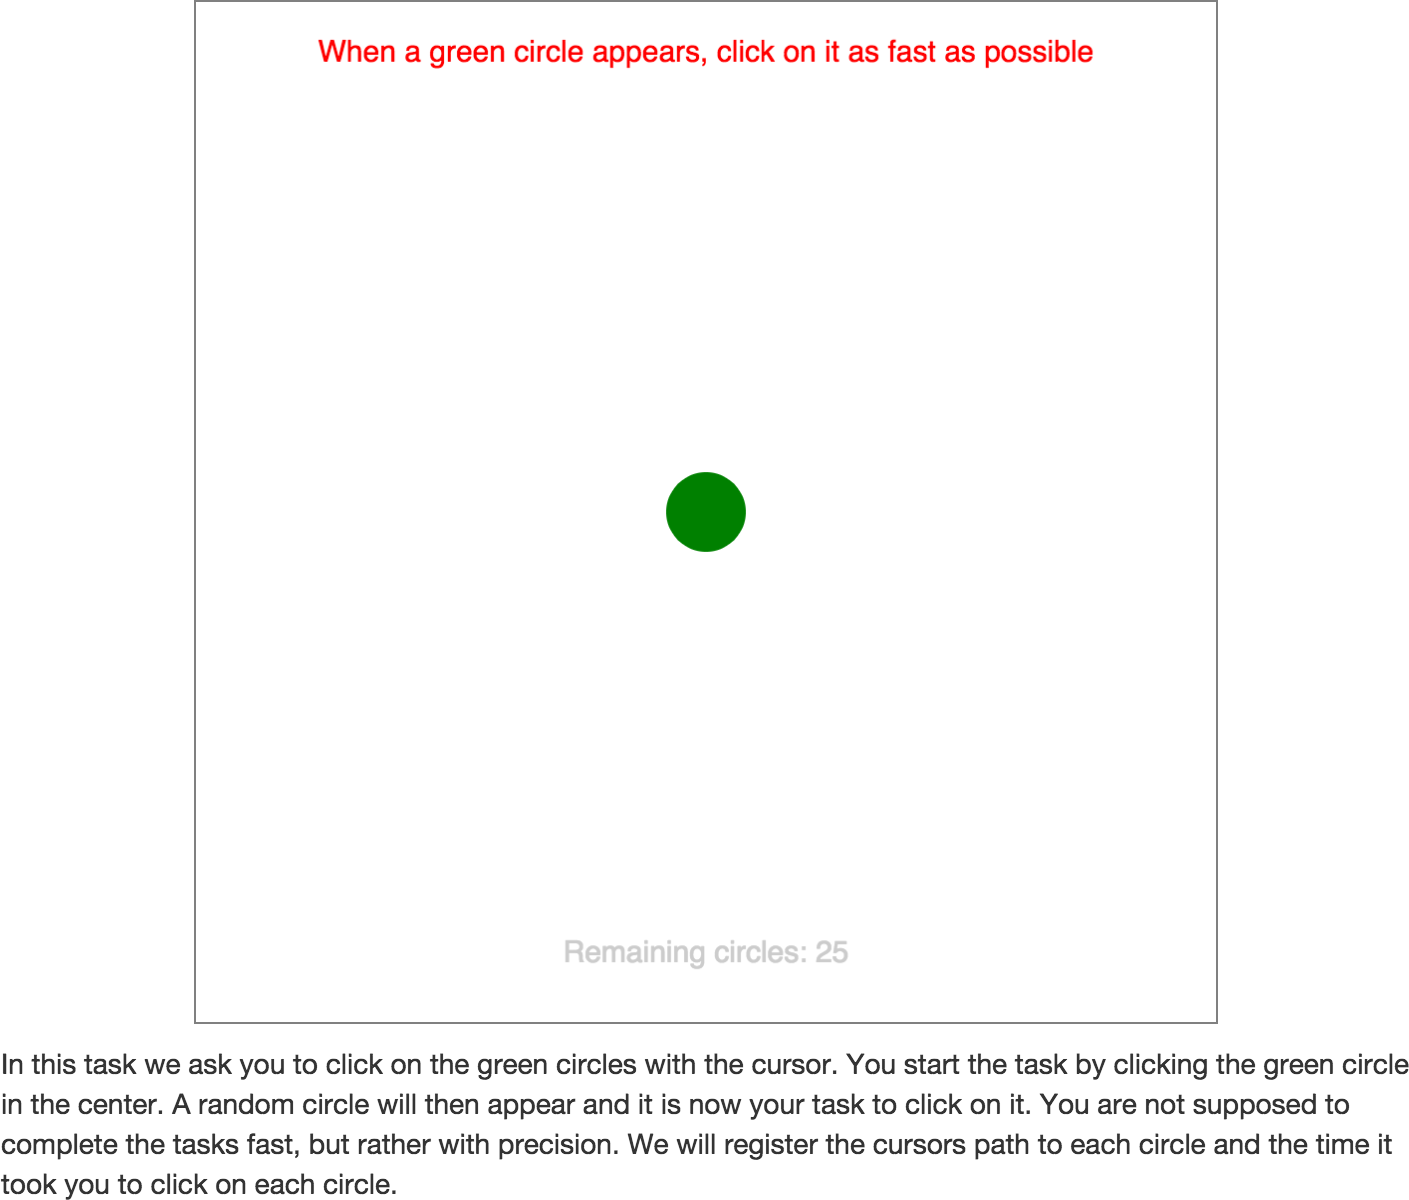
\includegraphics[width=0.8\textwidth, trim = 8cm 20cm 8cm 15cm, clip]{images/screenshots/ex_step_6_pointing_start}
\label{fig:pegeopgave_start}
\caption{Illustration af centercirklen, og målet der skal rammes efter der klikkes på cirklen I midten af skærmen}
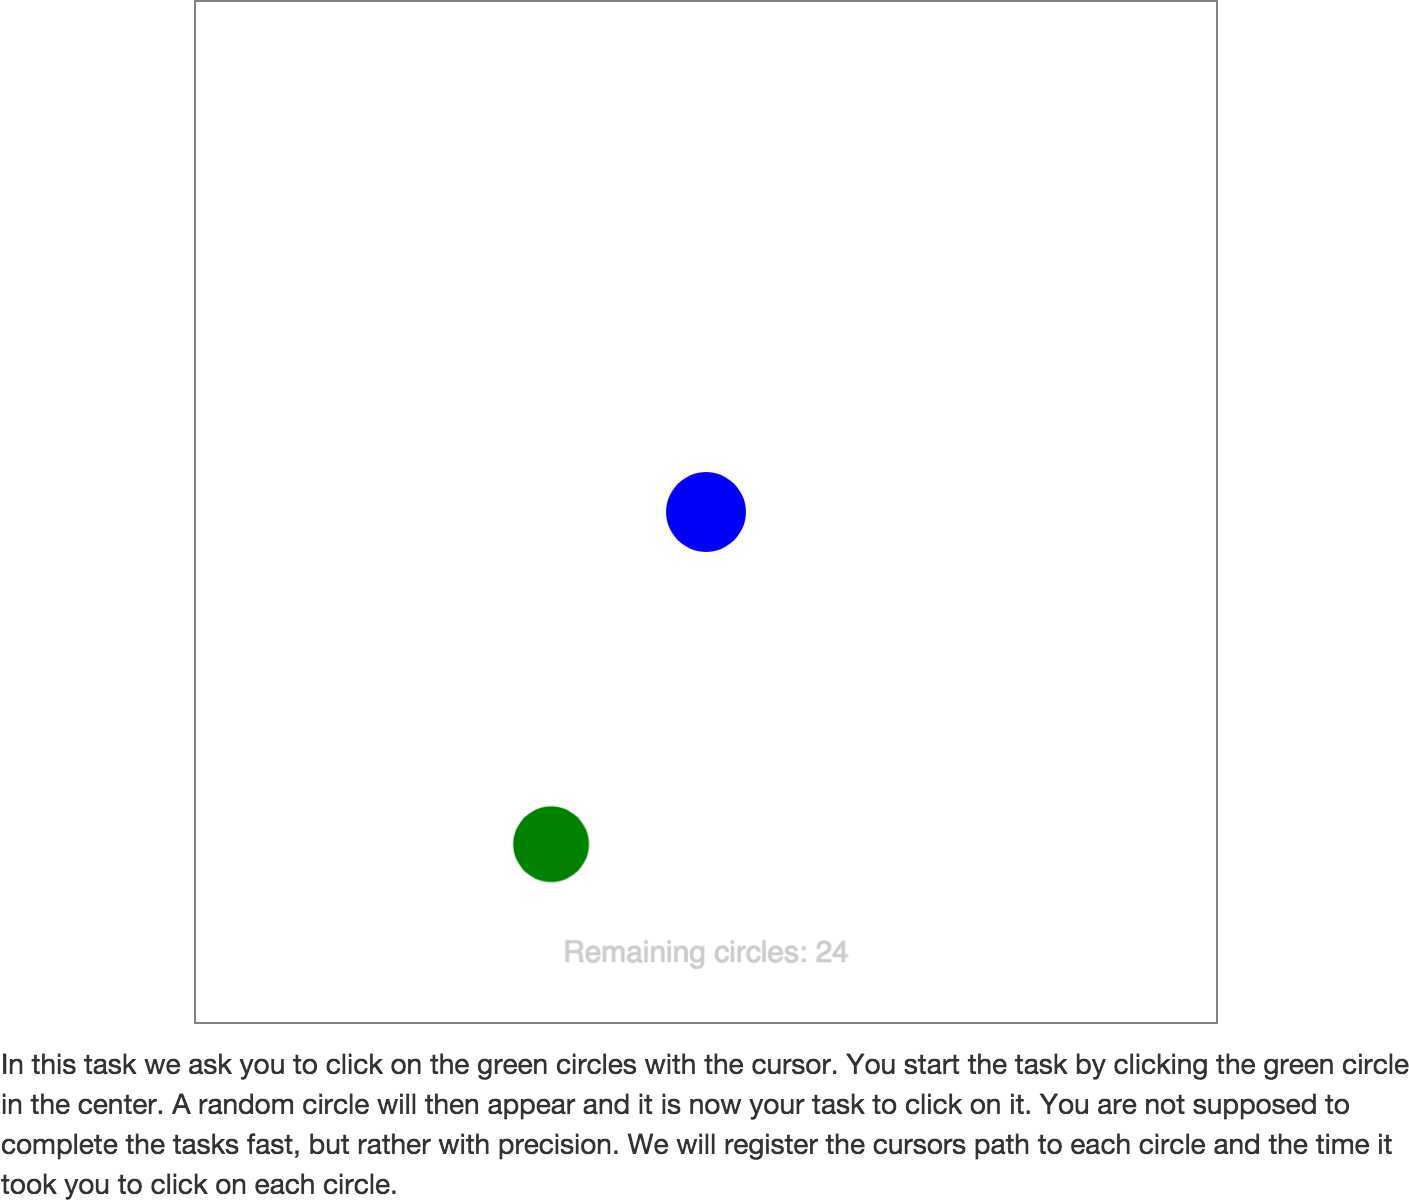
\includegraphics[width=0.8\textwidth, trim = 8cm 8cm 8cm 15cm, clip]{images/screenshots/ex_step_6_pointing_target_1}
\label{fig:pegeopgave_target}
\caption{Illustration af centercirklen, målet der skal rammes, og stien som testpersonen har taget for at komme hen til målet}
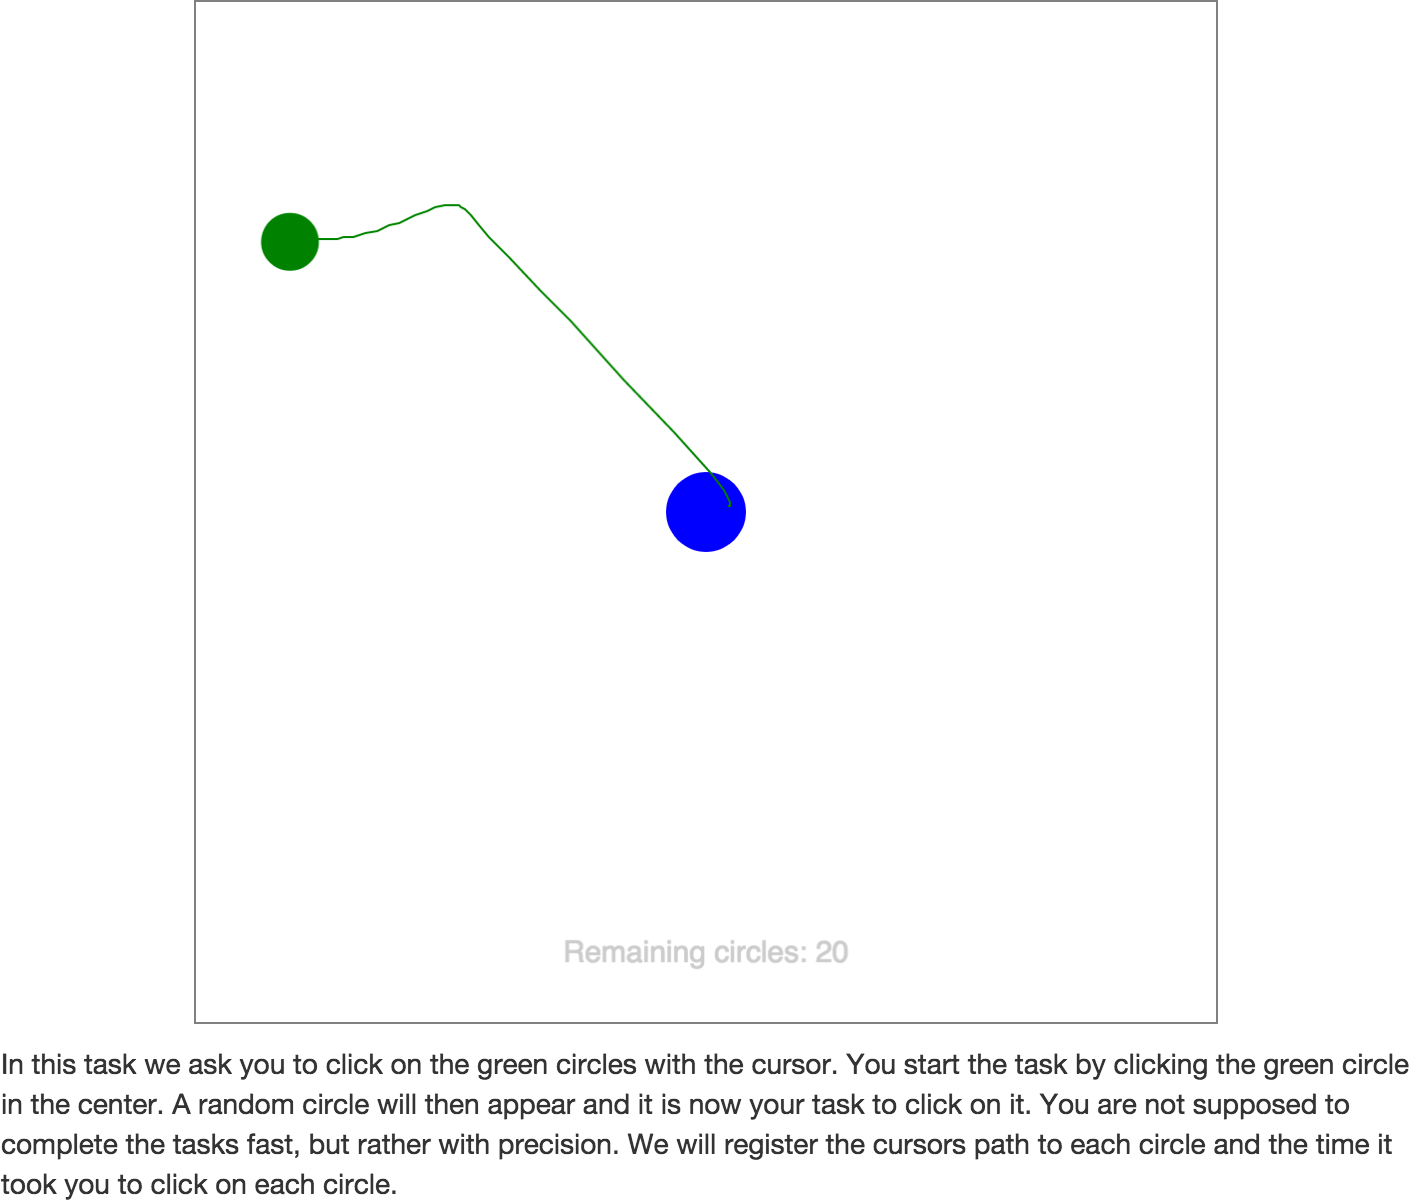
\includegraphics[width=0.8\textwidth, trim = 8cm 22cm 20cm 5cm, clip]{images/screenshots/ex_step_6_pointing_path}
\label{fig:pegeopgave_path}
\end{minipage}
\begin{minipage}[t]{.5\linewidth}
\centering
\vspace{0pt}
    \begin{tabular}{ c c c c }
        Forsøg & $A$ & $W$ & $A/W$ \\\hline
        1  & 67  & 20 & 3.35  \\
        2  & 184 & 38 & 4.84  \\
        3  & 280 & 14 & 20.00 \\
        4  & 230 & 29 & 7.93  \\
        5  & 144 & 55 & 2.62  \\
        6  & 249 & 29 & 8.59  \\
        7  & 255 & 14 & 18.21 \\
        8  & 96  & 50 & 1.92  \\
        9  & 225 & 19 & 11.84 \\
        10 & 263 & 12 & 21.92 \\
        11 & 259 & 25 & 10.36 \\
        12 & 229 & 20 & 11.45 \\
        13 & 215 & 31 & 6.94  \\
        14 & 198 & 83 & 2.39  \\
        15 & 301 & 16 & 18.81 \\
        16 & 194 & 66 & 2.94  \\
        17 & 260 & 12 & 21.67 \\
        18 & 296 & 14 & 21.14 \\
        19 & 180 & 44 & 4.09  \\
        20 & 278 & 11 & 25.27 \\
        21 & 283 & 37 & 7.65  \\
        22 & 40  & 32 & 1.25  \\
        23 & 233 & 10 & 23.30 \\
        24 & 191 & 50 & 3.82  \\
        25 & 179 & 18 & 9.94  \\\hline
    \end{tabular}
   \captionof{table}{Størrelser i pixels af $A$ (længde til mål), $W$ (bredde af mål) og udregnede $A/W$ for alle pegeopgaver}
   \label{tab:pegeopgave}
\end{minipage}

\newpage
\addcontentsline{toc}{subsection}{Generelt for de tre opgaver}
\subsection*{Generelt for de tre opgaver}
I alle opgaverne vil testdeltagerne blive informeret om, hvor mange opgaver de mangler at gennemføre, så de ved hvornår de er færdige. Den grå tekst \textit{"Remaining circles"} i figur \ref{fig:pegeopgave_target} er et eksempel på, hvordan denne information så ud undervejs. Vi har medtaget det i håb om, at testdeltagere fra crowdsourcing forsøget ikke vil miste tålmodigheden midt i testen.  

Hvis testdeltagerne bevæger pegeenheden uden for det canvas som opgaven skal udføres i, vil denne del af banen ikke komme med i vores gemte data. For tunnel- og spiralopgaverne er størrelsen på det omkringliggende canvas 1024x512 pixels, imens det for pegeopgaven er 512x512 pixels. Disse størrelser er faste uanset størrelsen på testdeltagerens skærm. Hvilket er valgt for at sikre de samme forhold på elementerne i opgaverne for alle testdeltagere.

\addcontentsline{toc}{chapter}{Eksperimenter}
\chapter*{Eksperimenter}

\addcontentsline{toc}{section}{Udførsel af eksperimenter}
\section*{Udførsel af eksperimenter}

\addcontentsline{toc}{subsection}{Laboratorieeksperiment}
\subsection*{Laboratorieeksperiment}
Laboratorieeksperimentet vil blive udført af 10 tilfældigt udvalgte universitetsstuderende - dog ikke dataloger.
Forsøget foretages fra kl 9-13 - tidligt på dagen - for at sikre, at folk stadig er friske. Det vil foregå i en 4-personers sofabås på H.C. Ørsted instituttet, hvor der er privat og få forstyrrelser.

Der vil være afsat 20 minutter til hver deltager, dog med plads til ekstra tid hvis nødvendigt. For at sikre os, at forsøgene forløber korrekt og ensartet har vi udarbejdet en drejebog, der kan ses i bilag \ref{sec:drejebog}. Hver deltager bliver først introduceret til vores projekt og derefter introduceret til henholdsvis tunnel-, spiral- og pegeopgaven.

Herefter bliver testdeltageren bedt om at udføre tunnelopgaven, efterfulgt af spiralopgaven og til sidst pegeopgaven. Der vil være et antal opgaver, som skal udføres henholdsvis fire tunnelopgaver, fire spiralopgaver og 25 pegeopgaver.

\addcontentsline{toc}{subsection}{Crowdsourcingeksperiment}
\subsection*{Crowdsourcingeksperiment}
Crowdsourcingeksperimentet vil foregå på internettet, og vi har derfor gjort vores program tilgængeligt online. På grund af de faste canvas størrelser vil alle besøg fra smartphones eller tablets blive blokeret, og informeret om, at forsøget kun er tilgængeligt fra en computer. 

Ved crowdsourcingeksperimentets start vil hver deltager udfylde formularen, som ses i figur \ref{fig:Questions}, før de kan fortsætte. Når formularen er udfyldt fortsætter deltageren til opgaverne. Her skal der, ligesom i laboratorieeksperimentet, udføres 4 tunnelopgaver, efterfulgt af 4 spiralopgaver og til sidst 25 pegeopgaver. Efter, at deltageren har udført alle opgaver vil personens data blive sendt til en server, hvorefter deltageren får en informationsmeddelelse, der takker dem for deres deltagelse.

Vi har valgt at dele vores eksperiment på et antal Reddit-sider, da det er et meget populært internetfora og muliggør, at vi kan nå ud til så mange mennesker som overhovedet muligt.
\begin{itemize}
\item \url{reddit.com/r/denmark}
\end{itemize}
Vi valgte $/r/denmark$ fordi det er et aktivt subreddit, som passer til vores forespørgsel, med næsten hundredetusind unikke visninger per måned. 

For at nå ud til andet end danske brugere har vi også valgt at bruge de to følgende subreddits. De er beregnet til at spørge folk om hjælp, og er de to største med dette formål som vi har kunne finde.
\begin{itemize}
\item \url{reddit.com/r/helpme}
\item \url{reddit.com/r/care}
\end{itemize}

Vi vil også dele forsøget på vores egne Facebook-profiler. Teksten som vi brugte til at dele forsøget kan ses i bilag \ref{sec:crowdsource-text}, den engelske version blev brugt på Reddit, imens den danske blev brugt på Facebook.
\begin{figure}[h]
\centering
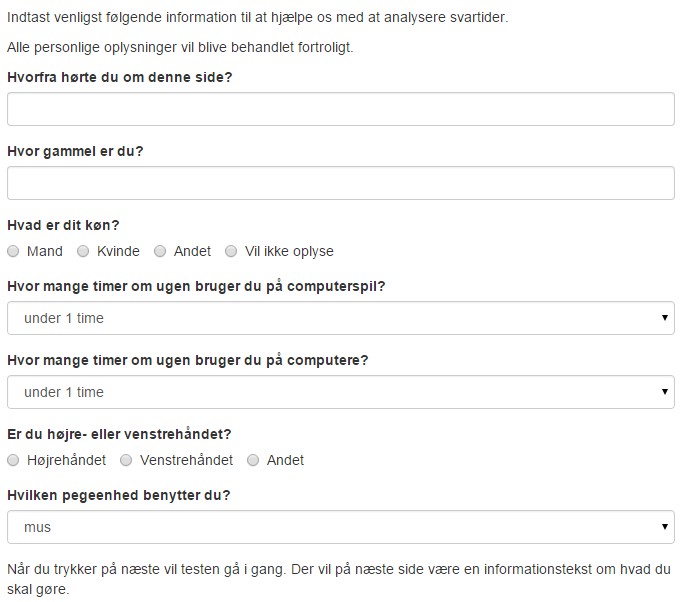
\includegraphics[width=.5\linewidth, trim = 0cm 0cm 7cm 0cm, clip]{images/screenshots/ex_questions}
\caption{Skærmbillede af spørgsmål som blev stillet før crowdsourcing-deltagerne kunne udføre forsøget}
\label{fig:Questions}
\end{figure}

\addcontentsline{toc}{section}{Resultat af eksperimenter}
\section*{Resultat af eksperimenter}

\addcontentsline{toc}{subsection}{Laboratorieeksperiment}
\subsection*{Laboratorieeksperiment}
Vi, P1, P2 og P3, udførte vores laboratorieeksperiment den 20. april 2015 på H.C. Ørsted instituttet. På trods af, at der på dagen ikke var mange mennesker til stede, fik vi alligevel 10 personer igennem vores eksperiment i løbet af fire timer. De 10 testdeltagere var af varierende nationalitet, og begge køn var repræsenteret. Alle testdeltagere blev hvervet af P1 og blev derefter introduceret til eksperimentet af enten P2 eller P3. Herefter udførte alle testdeltagere forsøget uden behov for yderlig assistance. Testdeltagerne syntes godt om forsøget, og forsøget forløb uden problemer eller forstyrrelser.

\addcontentsline{toc}{subsection}{Crowdsourcingeksperiment}
\subsection*{Crowdsourcingeksperiment}
Forsøget gik godt - 264 personer gennemførte vores forsøg og har suppleret os med data. Vi fik delt vores forsøg på størstedelen af de tidligere beskrevne sider, dog med nogle få undtagelser. Generelt set var Reddit det mest lukrative sted, hvorfra 140 personer har skrevet siden på som deres reference - hvorimod 74 skrev, at de var blevet refereret fra Facebook.

Det var ikke muligt at dele vores forsøg på \url{reddit.com/r/helpme} og \url{reddit.com/r/care}, da vi ikke havde nok 'karma'-point til at kunne lave et indlæg på disse sites.

Efterfølgende har vi lukket for muligheden for at deltage i vores forsøg den 30/04/2015, og skrevet en besked på forsøgssiden, hvor vi takker folk for deres deltagelse.

Vi har ved bachelorprojektets aflevering igen åbnet for adgang til forsøgssiden, dog uden mulighed for indsendelse af data.

\addcontentsline{toc}{chapter}{Analyse}
\chapter*{Analyse}
I dette afsnit vil vi analysere den indsamlede data ved brug af både kvantitative og kvalitative metoder. Mere præcist vil vi analysere testdeltagernes bevægelsesbaner og hastighedsprofiler. Afsnittet \textit{Modeludvælgelse} vil kun blive gennemgået kursorisk.

Den tilsvarende R-kode, som er brugt til analysen, kan findes i bilag \ref{sec:r-code}.
\addcontentsline{toc}{section}{Modeludvælgelse}
\section*{Modeludvælgelse}
Som det kan ses af de fire formuleringer for Fitts' lov, kan alle fire opfattes som affine modeller, med tiden $T$ som y-variabel og ID som x-variabel. Bemærk, at Welfords formel har en skæring med y-aksen i 0, dvs. $y=b\cdot x$.

For at kunne finde ud af, hvilken af de fire affine modeller, der beskriver vores data bedst, har vi taget udgangspunkt i \cite{wu2011experiments}, som refererer til tre modeludvælgelseskriterier som værende almindeligt anvendte.

I \cite{wu2011experiments} afsnit 1.7 bliver $C_p$, $AIC$ og $BIC$ beskrevet som almindeligt anvendte, og der bliver refereret til Occham's Razor som værende et godt udgangspunkt ved modeludvælgelse, da det oftest er den simpleste model der passer bedst. Dette har vi brugt til selv at vælge $LSE$, da denne er simpel, og derfor er understøttet som metode af Occham's Razor.
\begin{itemize}
\item{Least Squared Errors (LSE) \cite{legendre1805}}
\item{Mallow's $C_p$ \cite{mallow1973}}
\item{Akaike Information Criterion (AIC) \cite{akaike1973}}
\item{Bayesian Information Criterion (BIC) \cite{schwarz1978}}
\end{itemize}
LSE beregnes ved at finde gennemsnittet af kvadratet på afstandene fra punkterne til modellen. Den model som har det laveste gennemsnit bliver vurderet som bedst. Et problem ved udelukkende at benytte dette kriterium er, at en model altid kan beskrive alle datapunkter perfekt ved blot at inkludere flere parametre. Således, at modellen bliver et polynomium af højere grad end det originale. Dette er overfitting.

Mallow's $C_p$-kriteriet bliver beregnet ud fra LSE men inddrager også antallet af parametre i beregningen for netop at undgå overfitting. Tilsvarende gør sig gældende for AIC og BIC, de beregnes dog ved hjælp af maximum likelihood i stedet for LSE.

For et givent datasæt $x$ og en tilhørende statistisk model vil likelihoodfunktionen beregne sandsynligheden for, at modellens parametre $p$ vil resultere i $x$. Ved maximum likelihood findes den værdi for  $p$, som maksimerer likelihood funktionen. \textit{"Det vil sige den v{\ae}rdi af  p der gør den observerede v{\ae}rdi x mest sandsynlig"} \cite[s.14]{ditlevsen2011}. Forskellen på AIC og BIC er, at BIC vægter antallet af parametre mere negativt end AIC.

Af de fire beskrevne modeller har vi valgt at bruge AIC, da det er den mest udbredte. Hvis vi lader $L$ være maximum likelihood-værdierne for modellens parametre og $k$ antallet af parametre, så er AIC givet ved
\begin{align}
AIC = 2k - 2\ln(L) \label{eq:aic}
\end{align}
Vi har til vores analyse brugt programmeringssproget R, som både har lineær regression og AIC-funktionalitet indbygget. Funktionen $lm$\footnote{R dokumentation om $lm$: \url{https://stat.ethz.ch/R-manual/R-patched/library/stats/html/lm.html}} fitter en affin model ud fra de $(x,y)$ datasæt der gives som input. Modellen bliver baseret på least squares, og kan også tvinges til at gå gennem origo (for Welford).

Funktionen $AIC$\footnote{R dokumentation om $AIC$: \url{https://stat.ethz.ch/R-manual/R-patched/library/stats/html/AIC.html}} bruger (\ref{eq:aic}) til sine beregninger, og tager som input en model, der har metoden $logLik$\footnote{R dokumentation om $logLik$: \url{https://stat.ethz.ch/R-manual/R-patched/library/stats/html/logLik.html}}, hvilket $lm$'s output-modeller har. $lm$ og $AIC$ gør det derfor muligt at sammenligne modellerne med R.

\addcontentsline{toc}{section}{Indledende analyse}
\section*{Indledende analyse}
For at være sikre på, at vores data fra det ukontrollerede crowdsourcing eksperiment kan bruges til at sammenligne de fire formuleringer, har vi først kigget på vores 10 testdeltagere fra laboratieeksperimentet hver for sig. Vi har fitted vores 10 testdeltageres data fra pegeopgaverne til Fitts' lov hver for sig. To af disse plots kan ses i figur \ref{fig:testdeltager1} og \ref{fig:testdeltager3}.  Punkterne ligger tæt omkring modellen, angivet ved den blå linje, der er dog enkelte datapunkter bryder tendensen, specielt på figur \ref{fig:testdeltager3}.

Vi har derfor fjernet alle datapunkter, som afviger med mere end 3 gange standardafvigelsen, $\sigma$, som er kvadratroden af variansen på datasættet \cite{pearson1894}. Ved at filtrere data fra med for stor afvigelse, kan vi tilpasse en model, der beskriver størstedelen af vores data bedre. Figur \ref{fig:testdeltager7unfilter} og \ref{fig:testdeltager7filter} viser den tilpassede affine model for testdeltager 7 med og uden filtreret data.\\\\
\begin{minipage}{\linewidth}
	\begin{minipage}[b]{.45\linewidth}
		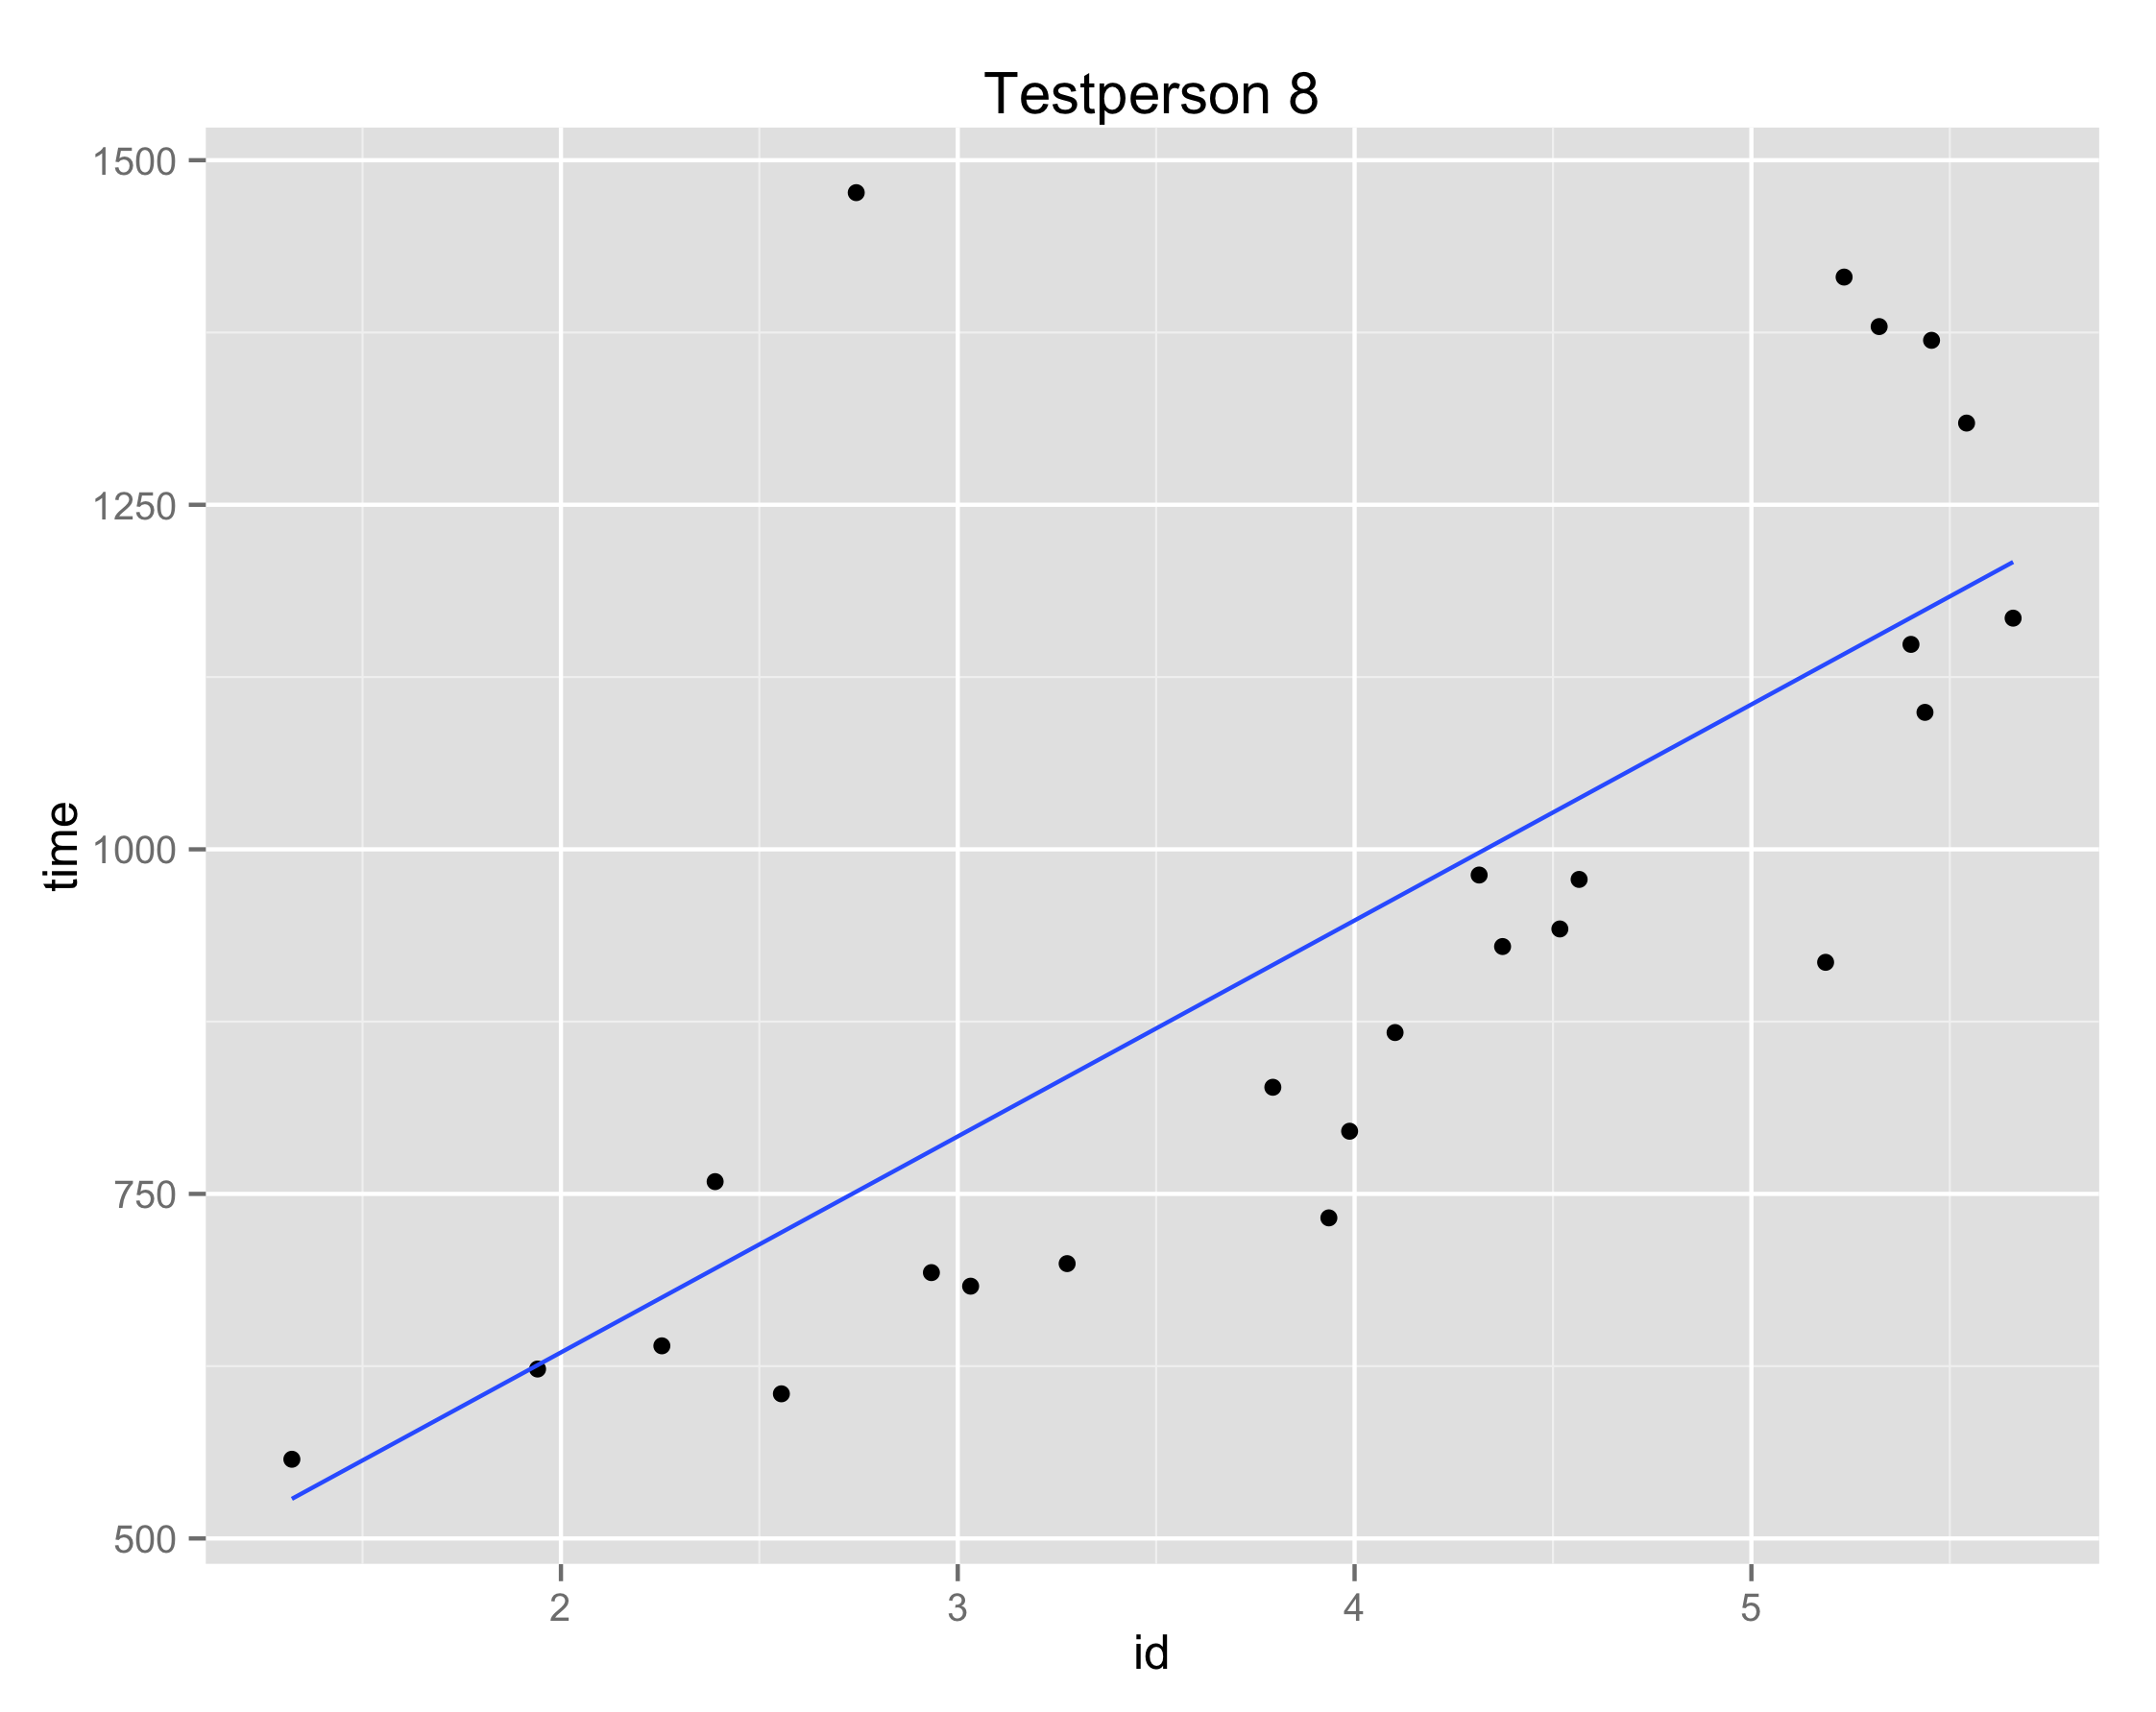
\includegraphics[width=\textwidth]{images/plots/plot_model_test_1}
		\captionof{figure}{Testdeltager 1's 25 pegeopgavedata med tiden ud af $y$-aksen og $ID$ på $x$-aksen}
		\label{fig:testdeltager1}
	\end{minipage}
	\begin{minipage}[b]{0.1\linewidth}
	~
	\end{minipage}
	\begin{minipage}[b]{0.45\linewidth}
		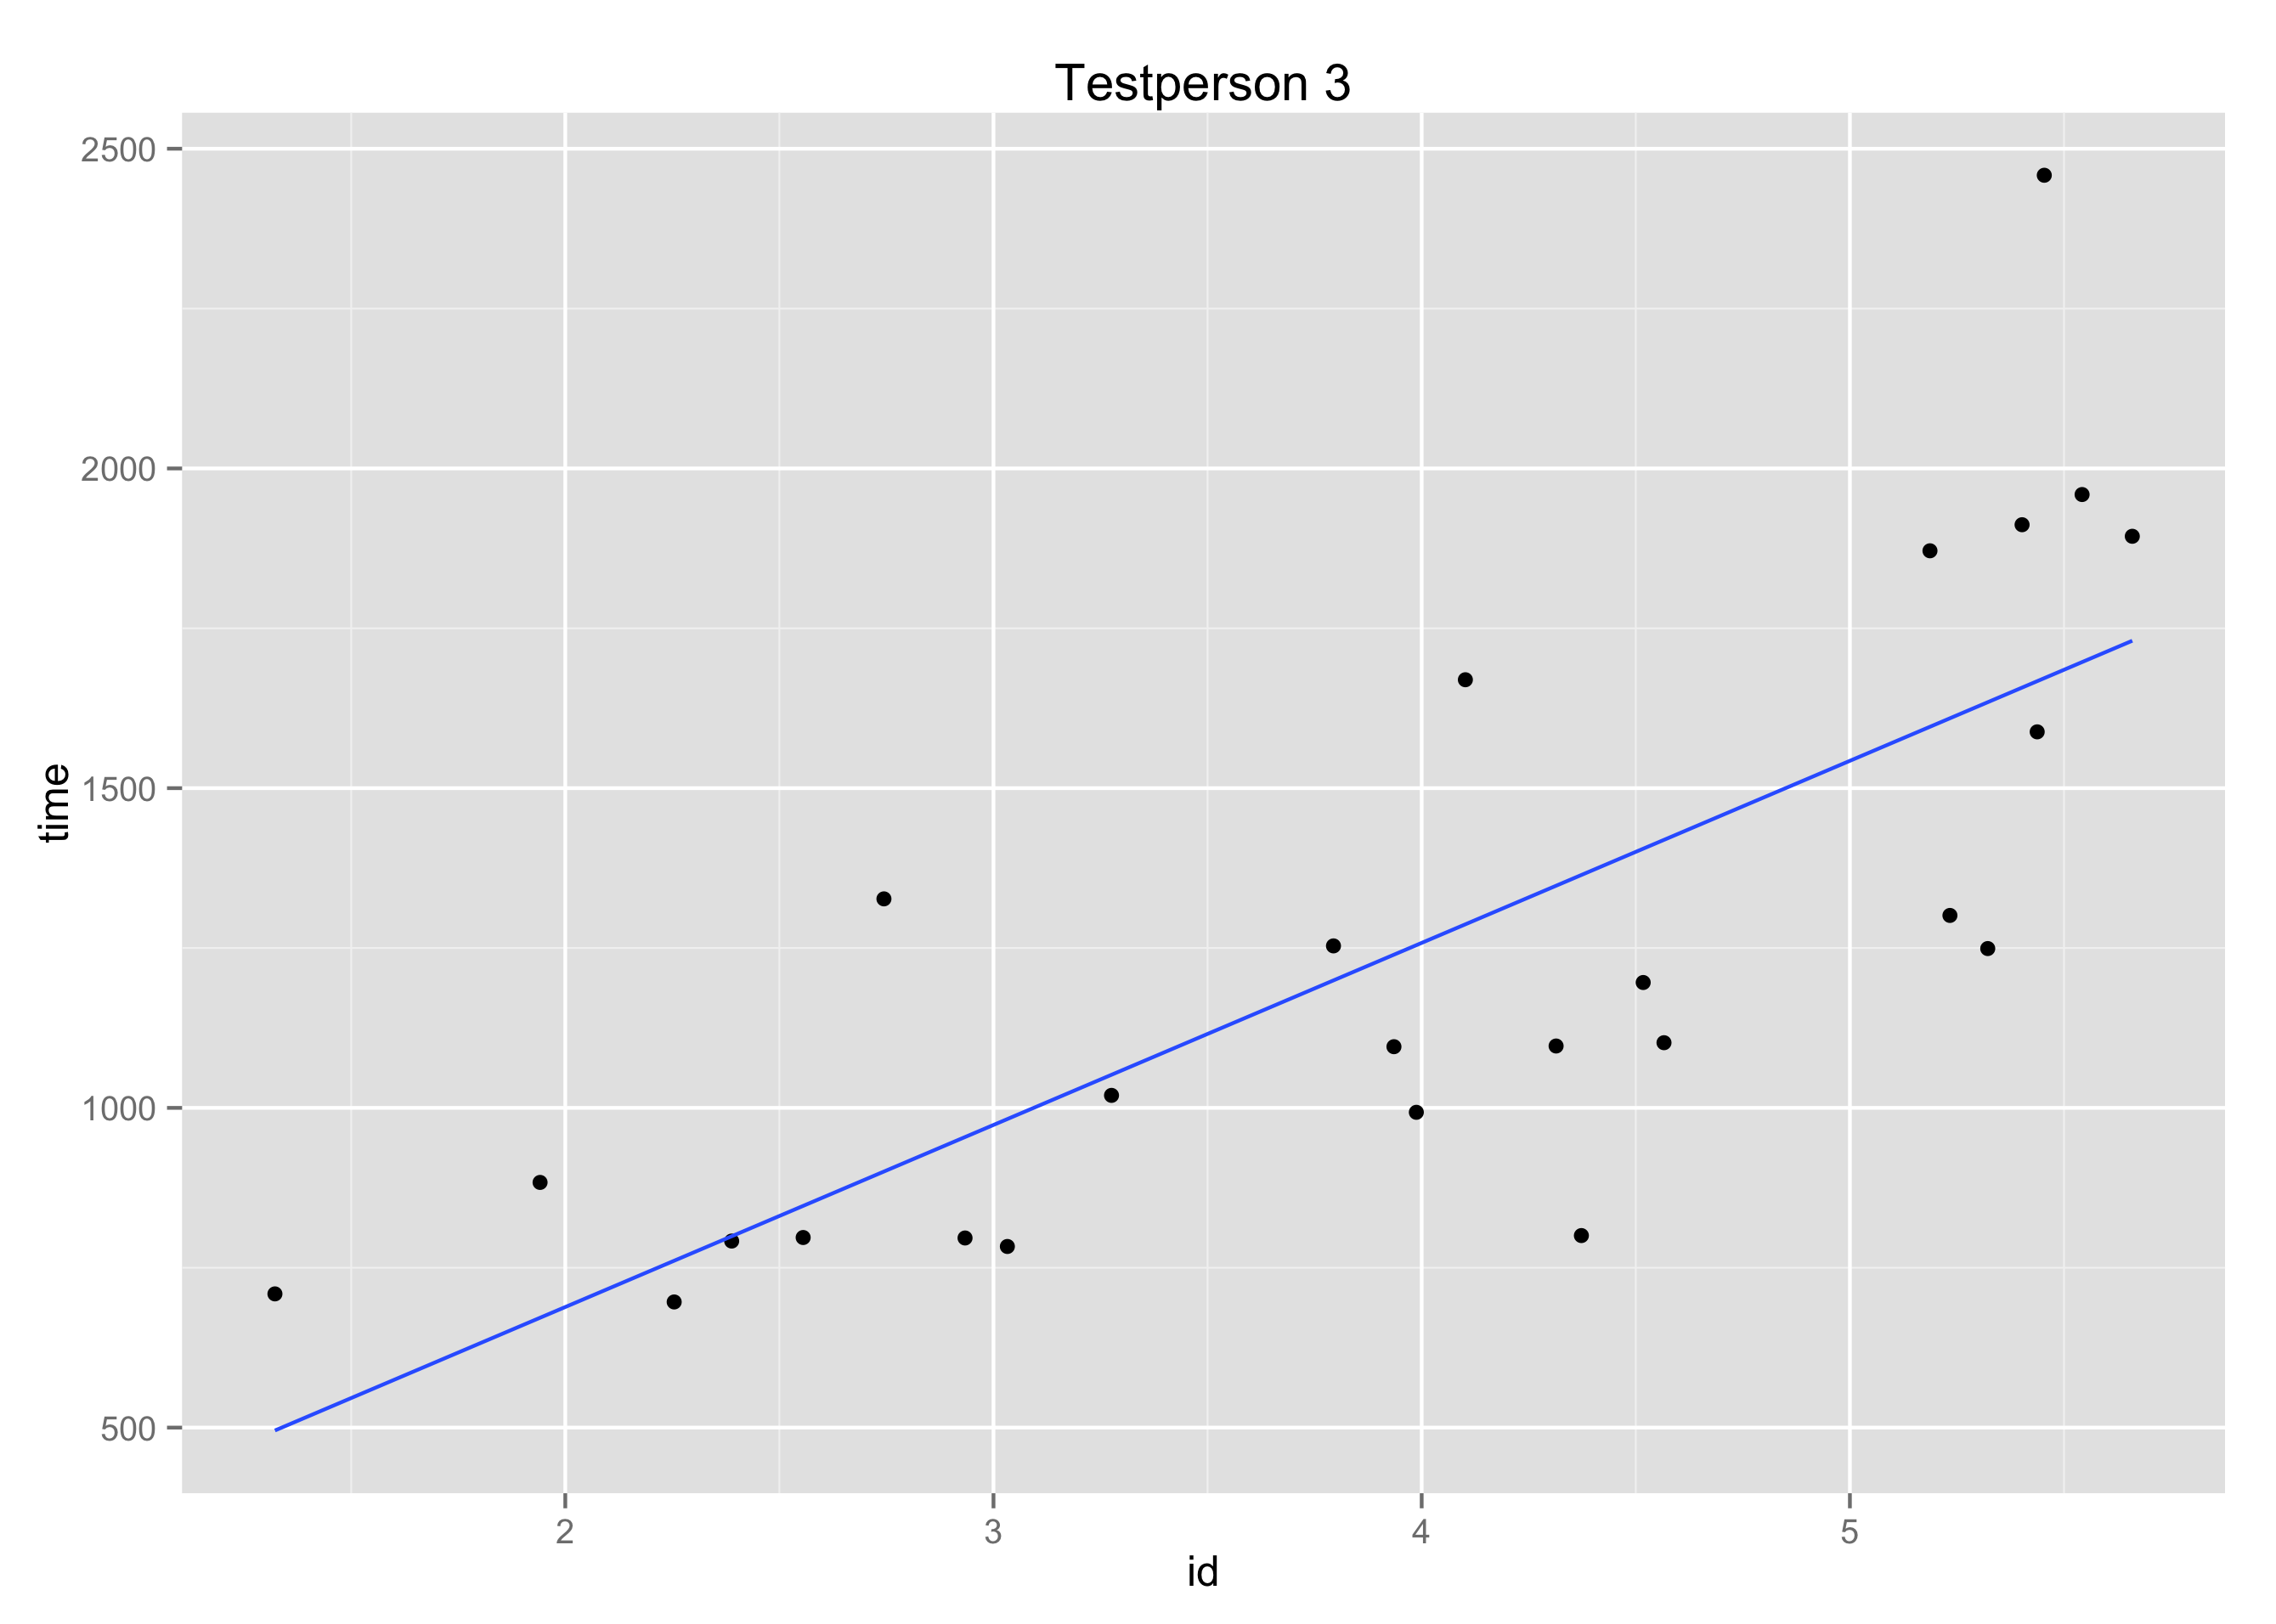
\includegraphics[width=\textwidth]{images/plots/plot_model_test_2}
		\captionof{figure}{Testdeltager 3's 25 pegeopgavedata med tiden ud af $y$-aksen og $ID$ på $x$-aksen}
		\label{fig:testdeltager3}
	\end{minipage}
\end{minipage}

\newpage
På baggrund af de affine linjers overenstemmelse med datapunkterne fra det kontrollerede eksperiment forventer vi, at dataene fra vores ukontrollerede forsøg også kan beskrives af de fire formuleringer. Vi vil derfor analysere de fire formuleringer af Fitts' lov med vores data fra det ukontrollerede crowdsourcingforsøg. Vores analyse vil basere sig på et filtreret datasæt ved den ovennævnte $\sigma$-metode, så eventuelle perifære data ikke medtages. I resten af analysen vil de 264 testdeltageres opgaver betyde den filtrerede del af det fulde datasæt.\\\\
\begin{minipage}{\linewidth}
	\begin{minipage}[t]{0.45\linewidth}
		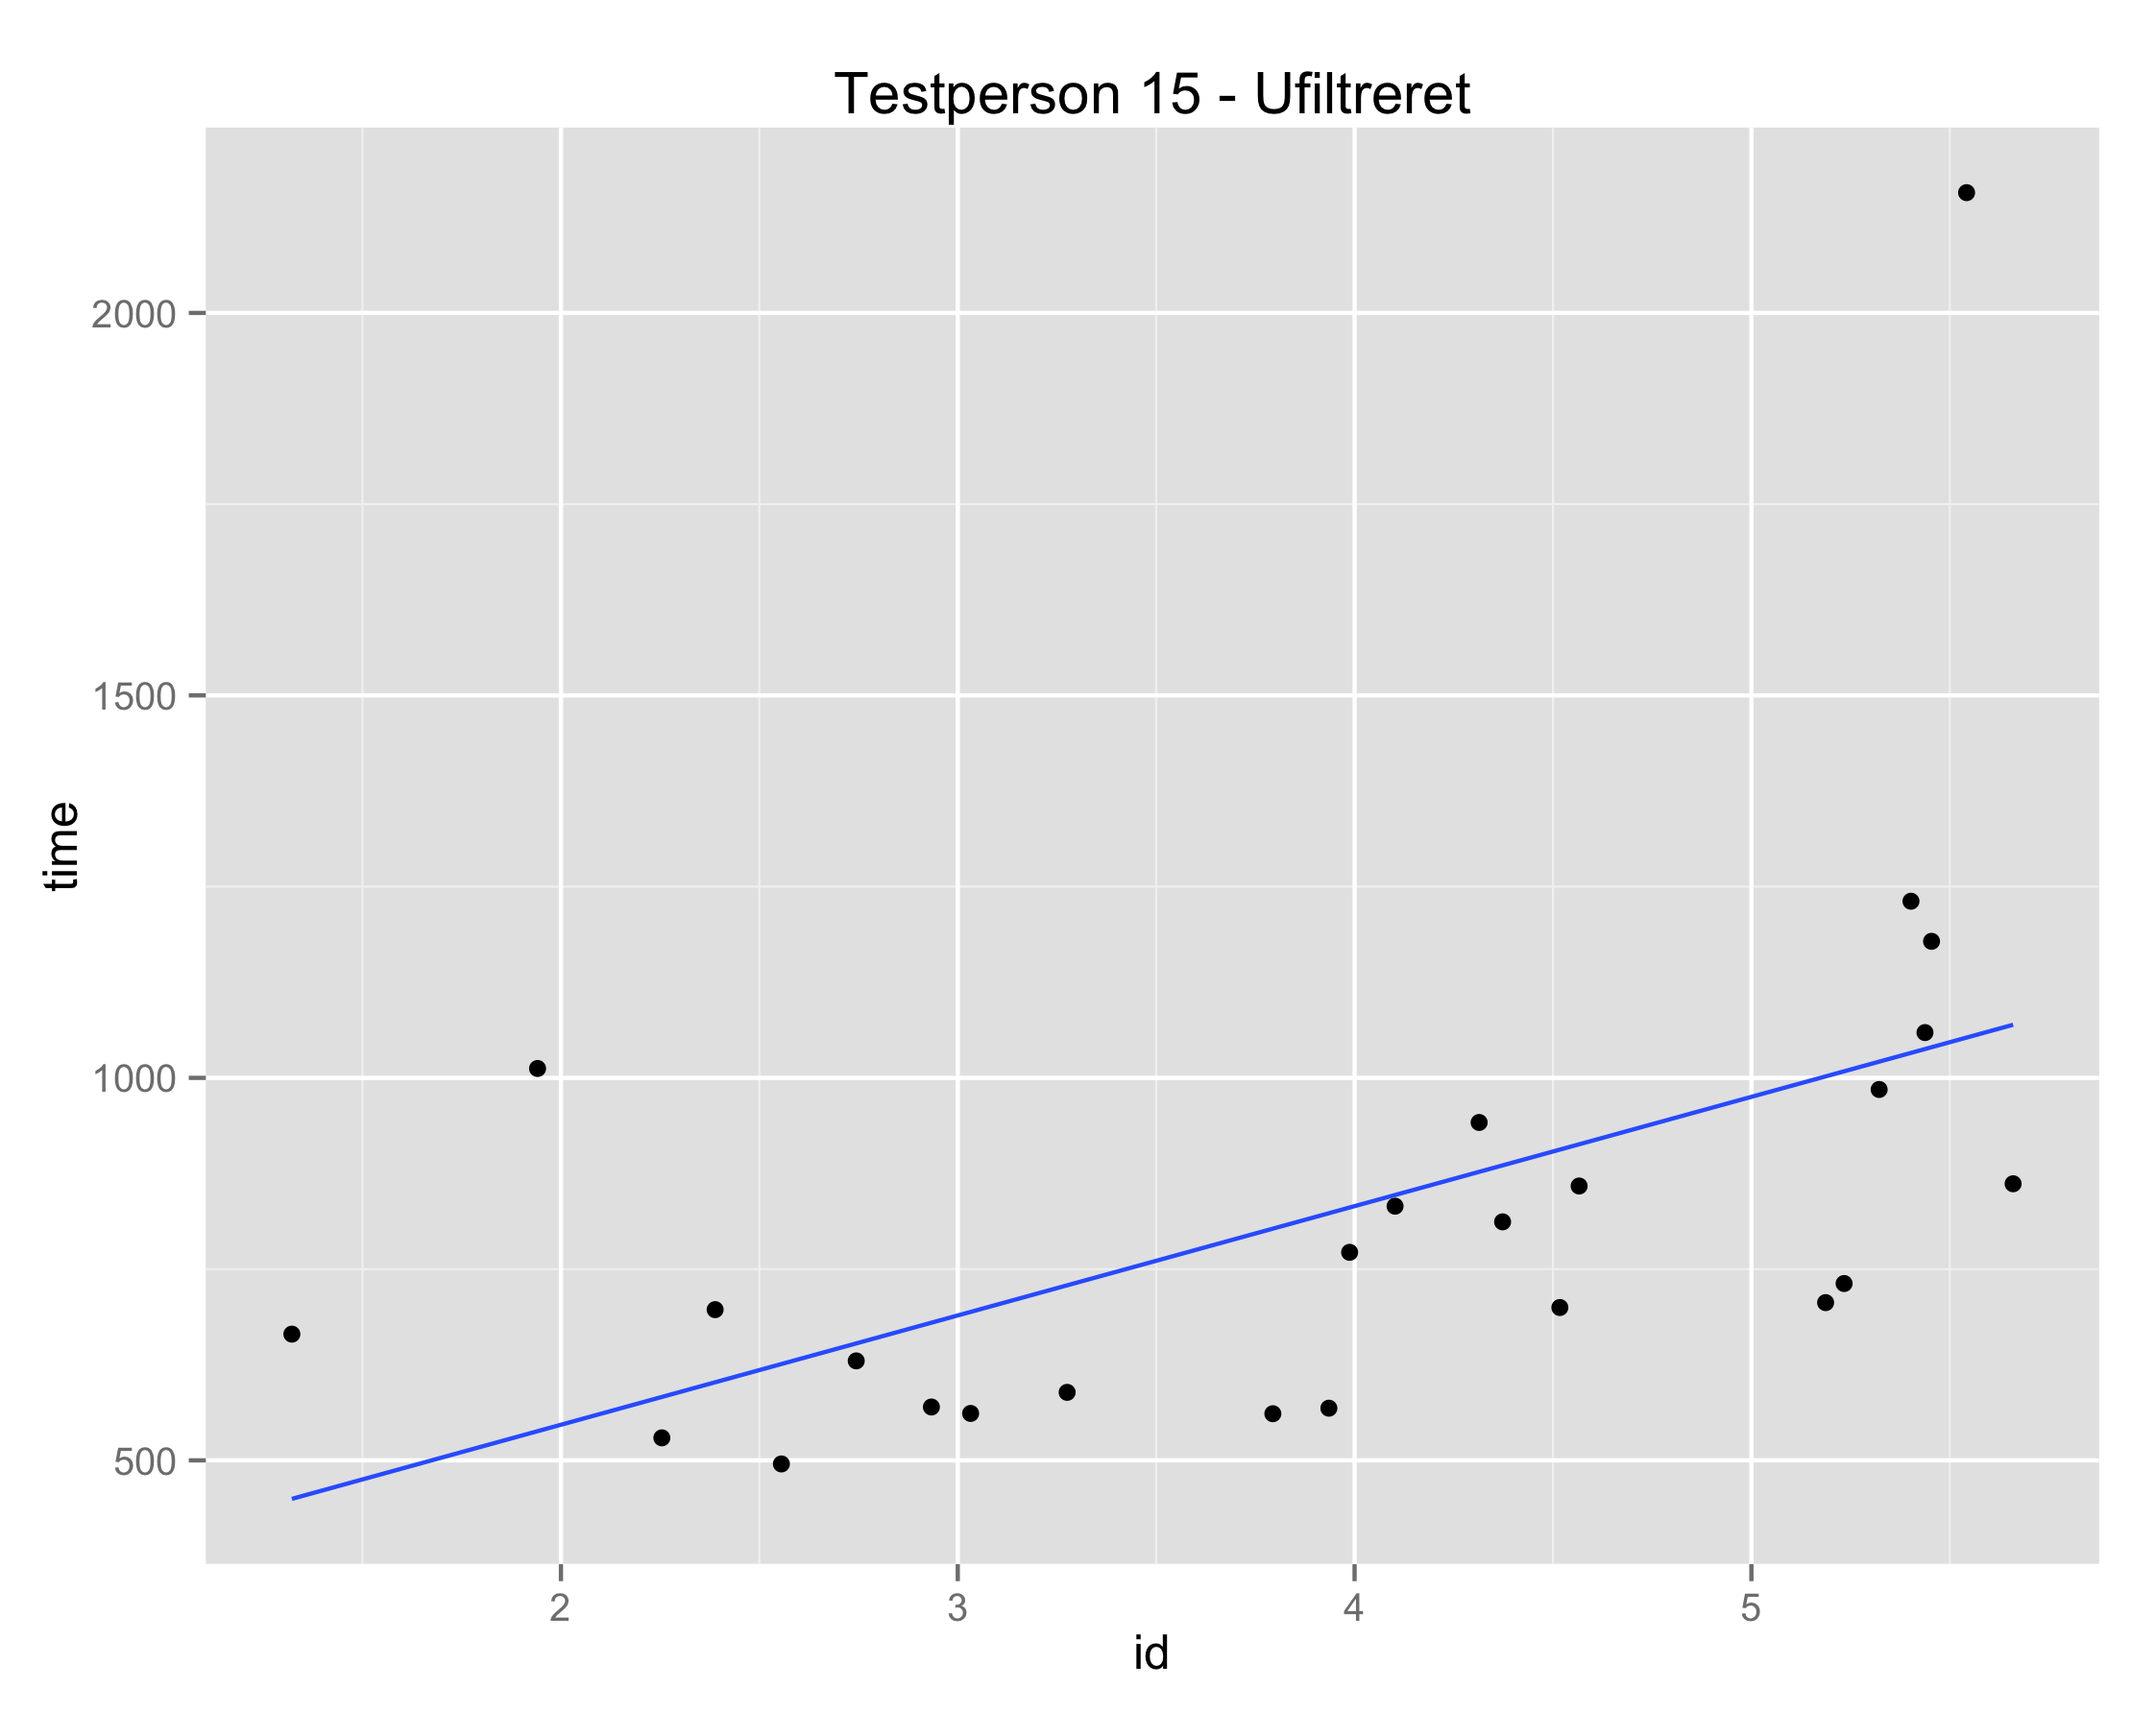
\includegraphics[width=\textwidth]{images/plots/plot_model_test_comparison_unfiltered}
		\captionof{figure}{Testdeltager 7's 25 pegeopgavedata uden nogen filtrering}
		\label{fig:testdeltager7unfilter}
	\end{minipage}
	\begin{minipage}[b]{0.1\linewidth}
	~
	\end{minipage}
	\begin{minipage}[t]{.45\linewidth}
		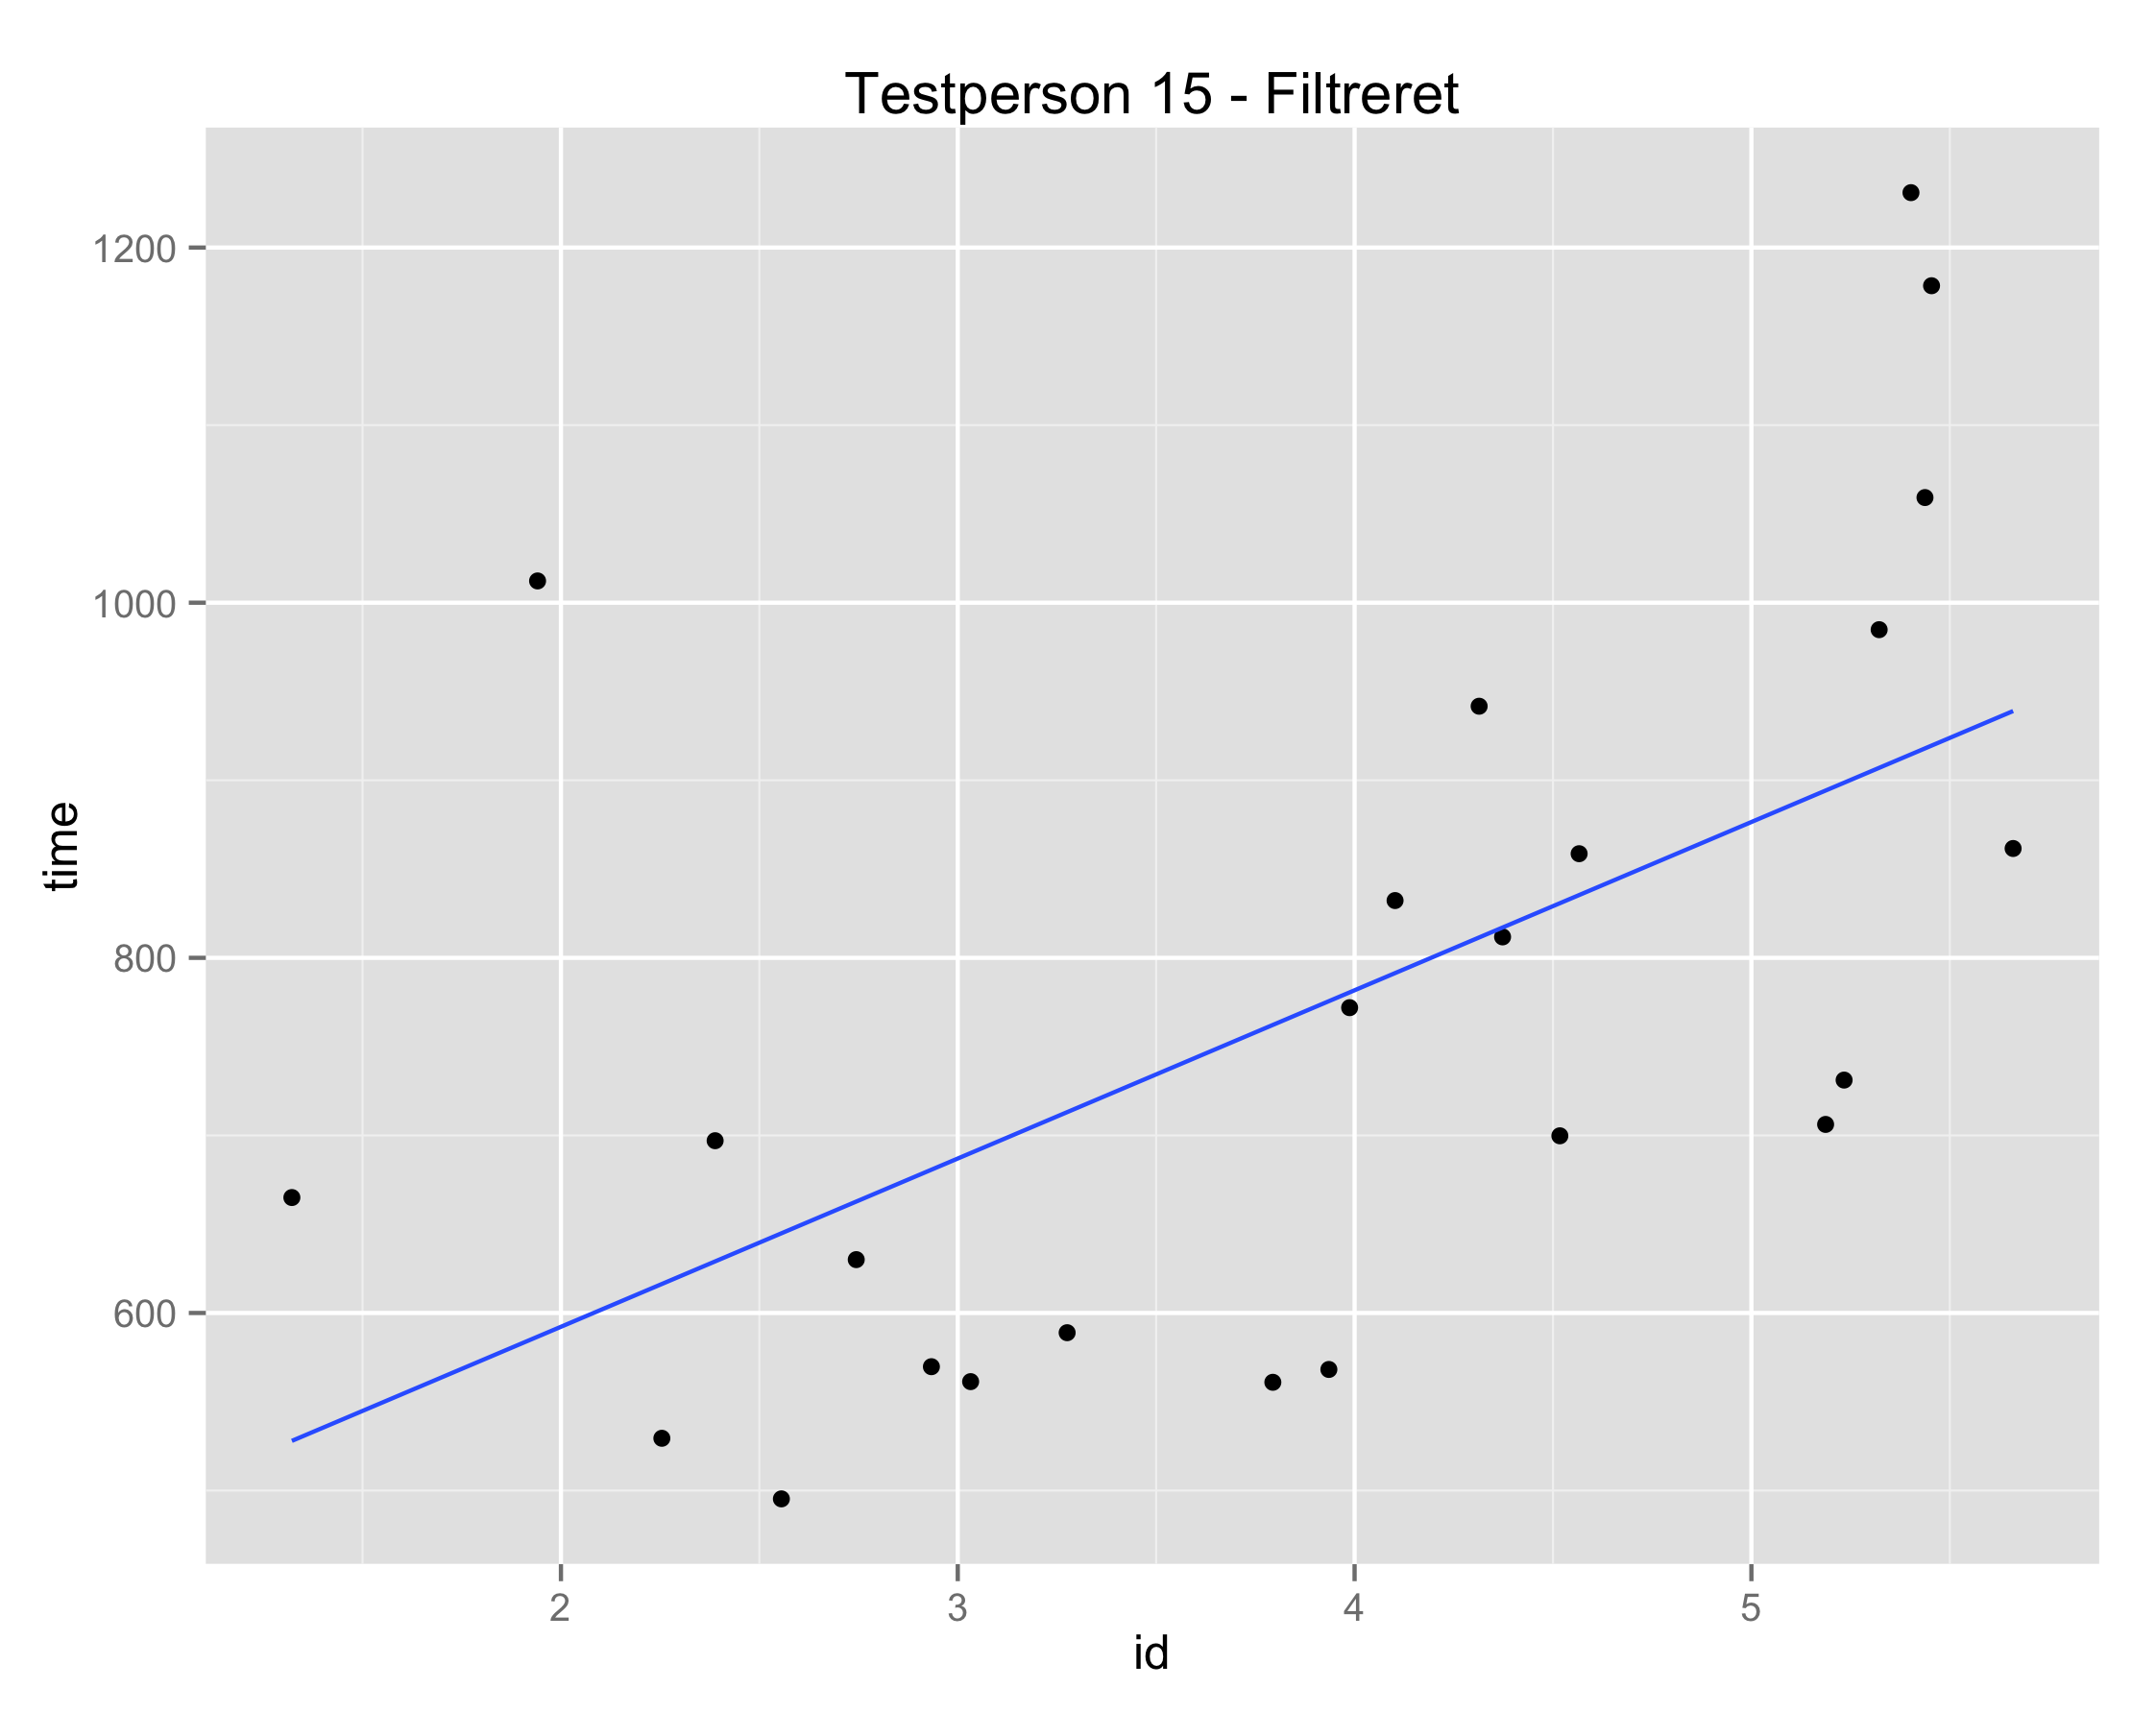
\includegraphics[width=\textwidth]{images/plots/plot_model_test_comparison_filtered}
		\captionof{figure}{Testdeltager 7's 25 pegeopgavedata med filtreret datasæt. Bemærk, at der kun er 24 datapunkter tilbage}
		\label{fig:testdeltager7filter}
	\end{minipage}
\end{minipage}

\addcontentsline{toc}{section}{Modelanalyse af pegeopgaver}
\section*{Modelanalyse af pegeopgaver}
Vores modelanalyse af pegeopgaver tager udgangspunkt i AIC-modellen og de datapunkter der er indsamlet ved crowdsourcingdeltagernes udførsel af opgaverne.

Hver af de fire formuleringer af Fitts' lov har vi tilpasset vores data fra de 264 testdeltageres pegeopgaver ved lineær regression. Til hver af modellerne har vi gjort brug af formuleringernes respektive $ID$ som $x$-koordinat og tiden, $t$, det tog testdeltageren at løse en pågældende pegeopgave som $y$-koordinat. De fire matematiske modeller med de tilpassede konstanter er vist nedenfor.
\begin{align*}
\text{Fitts': } &T = 392.29 + 149.42\cdot \log_2\left(\frac{2A}{W}\right)\\
\text{Welford's: } &T =  299.73\cdot \log_2\left(\frac{A+\frac{1}{2}W}{W}\right)\\
\text{Mackenzie's: } &T = 418.58 + 176.87\cdot \log_2\left(\frac{A+W}{W}\right)\\
\text{Meyer's: } &T = 504.48 + 157.13 \cdot \sqrt{\frac{A}{W}}
\end{align*}

Bemærk, at den additive konstant er målt i millisekunder lige som vores registrerede tider fra datasættet. Ud fra de tre additive konstanter, kan det ses, at testdeltagerne i gennemsnit bruger cirka 450 millisekunder på at opfange opgaven før de bevæger deres pegeenhed. Datapunkterne og de fire affine modeller er plottet og vist i figur \ref{fig:welford_affine_line}, \ref{fig:fitt_affine_line}, \ref{fig:meyer_affine_line} og \ref{fig:mackenzie_affine_line}. Hvert datapunkt er én testdeltagers tid ved en given opgaves $ID$. Bemærk, hvordan datapunkterne danner 25 vertikale 'søjler', én for hvert af vores pegeopgavers $ID$.

Det er de fire matematiske modeller som vores pegeopgaveanalyse vil tage udgangspunkt i. Ud fra modellerne og figurerne er det dog svært at sige noget om, hvilken af modellerne der klarer sig bedst i at beskrive datapunkterne. For at få et mere håndgribeligt resultat at analysere dette ud fra, vil vi gøre brug af en AIC-analyse og underbygge den med en residualanalyse.\\\\\begin{minipage}{\linewidth}
	\begin{minipage}[b]{0.45\linewidth}
		\captionof{figure}{Welford's lineære model med hans $ID$ ud af $x$-aksen og tiden ud af $y$-aksen}
		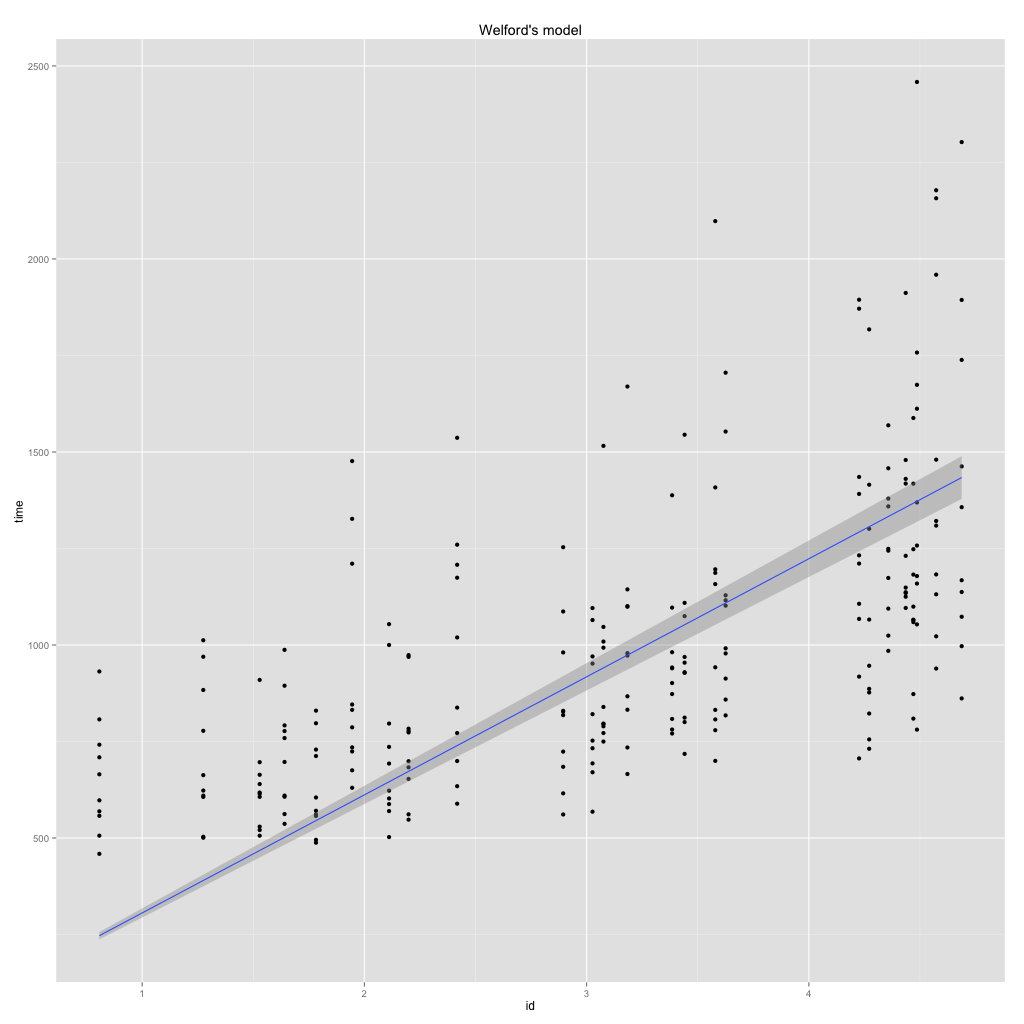
\includegraphics[width=\textwidth]{images/plots/plot_model_welford}
		\label{fig:welford_affine_line}
	\end{minipage}
	\begin{minipage}[b]{0.1\linewidth}
	~
	\end{minipage}
	\begin{minipage}[b]{0.45\linewidth}
		\captionof{figure}{Fitts' affine model med hans $ID$ ud af $x$-aksen og tiden ud af $y$-aksen}
		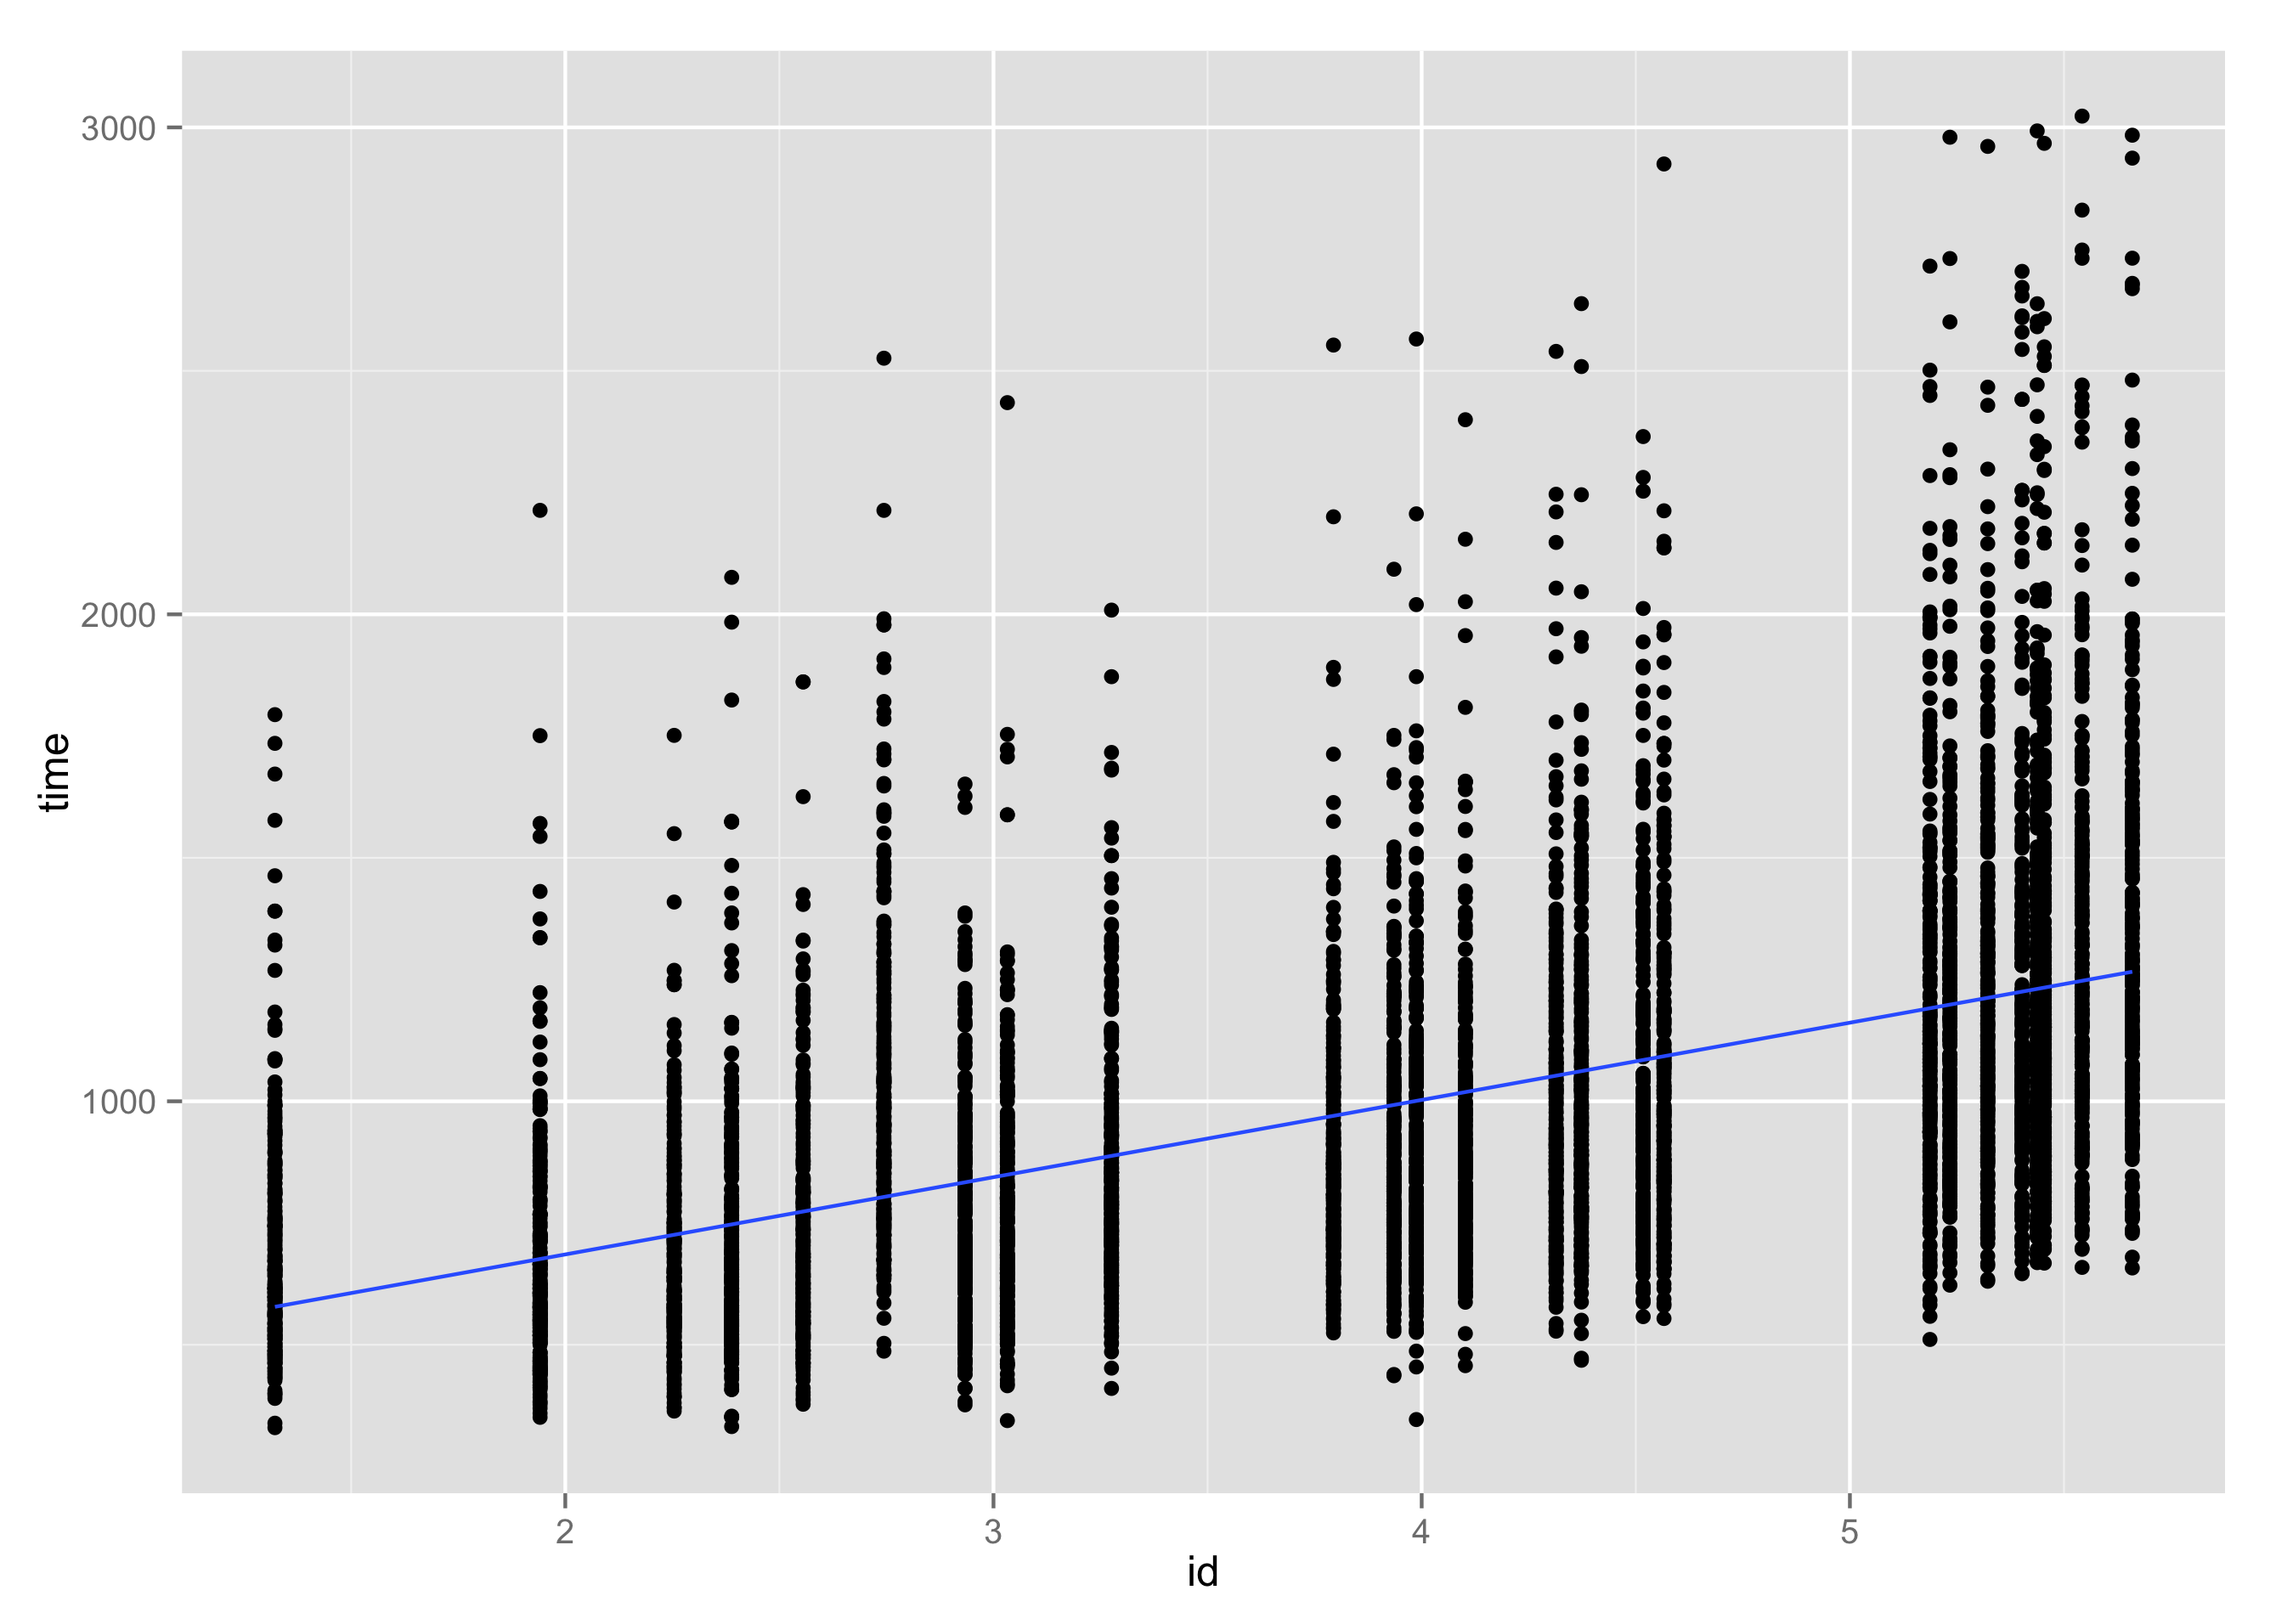
\includegraphics[width=\textwidth]{images/plots/plot_model_fitt}
		\label{fig:fitt_affine_line}
	\end{minipage}
	\begin{minipage}[b]{0.45\linewidth}
		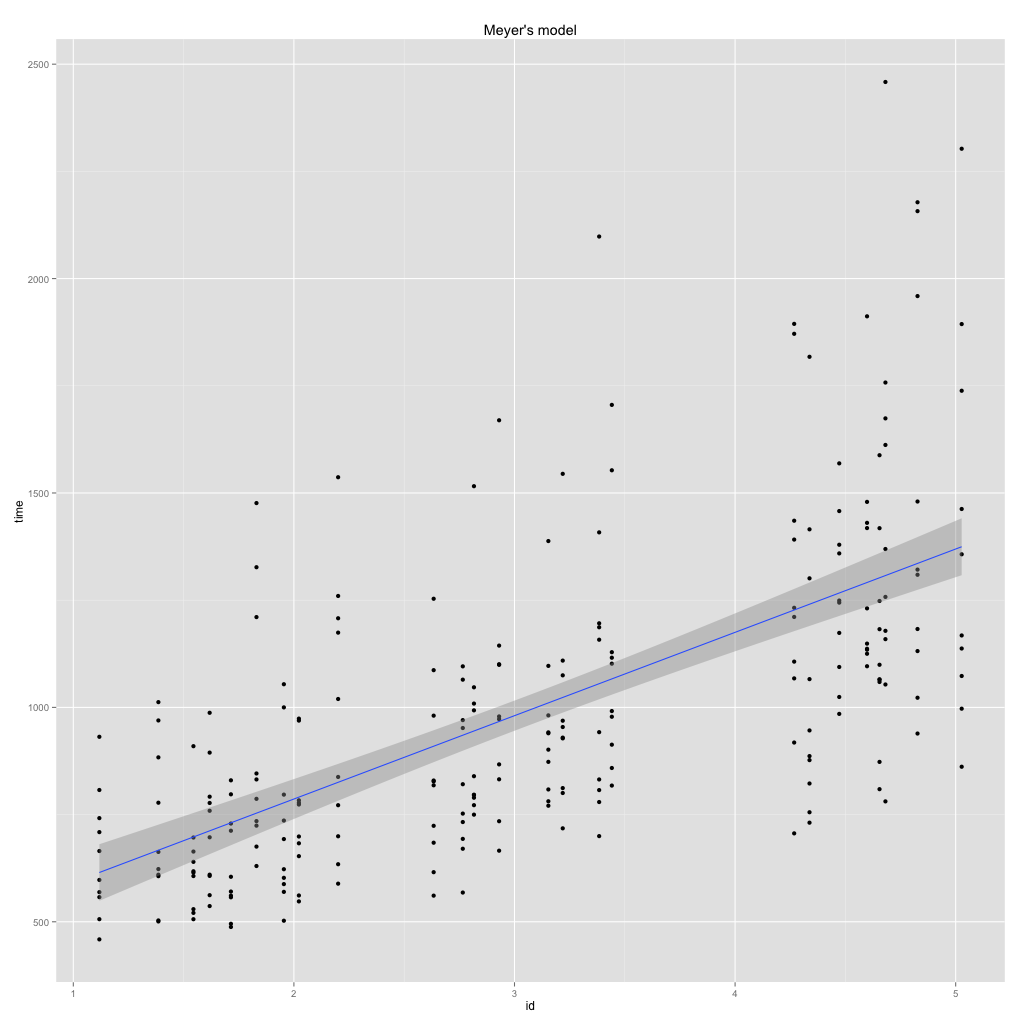
\includegraphics[width=\textwidth]{images/plots/plot_model_meyer}
		\captionof{figure}{Meyer's affine model med hans $ID$ ud af $x$-aksen og tiden ud af $y$-aksen}
		\label{fig:meyer_affine_line}
	\end{minipage}
	\begin{minipage}[b]{0.1\linewidth}
	~
	\end{minipage}
	\begin{minipage}[b]{0.45\linewidth}
		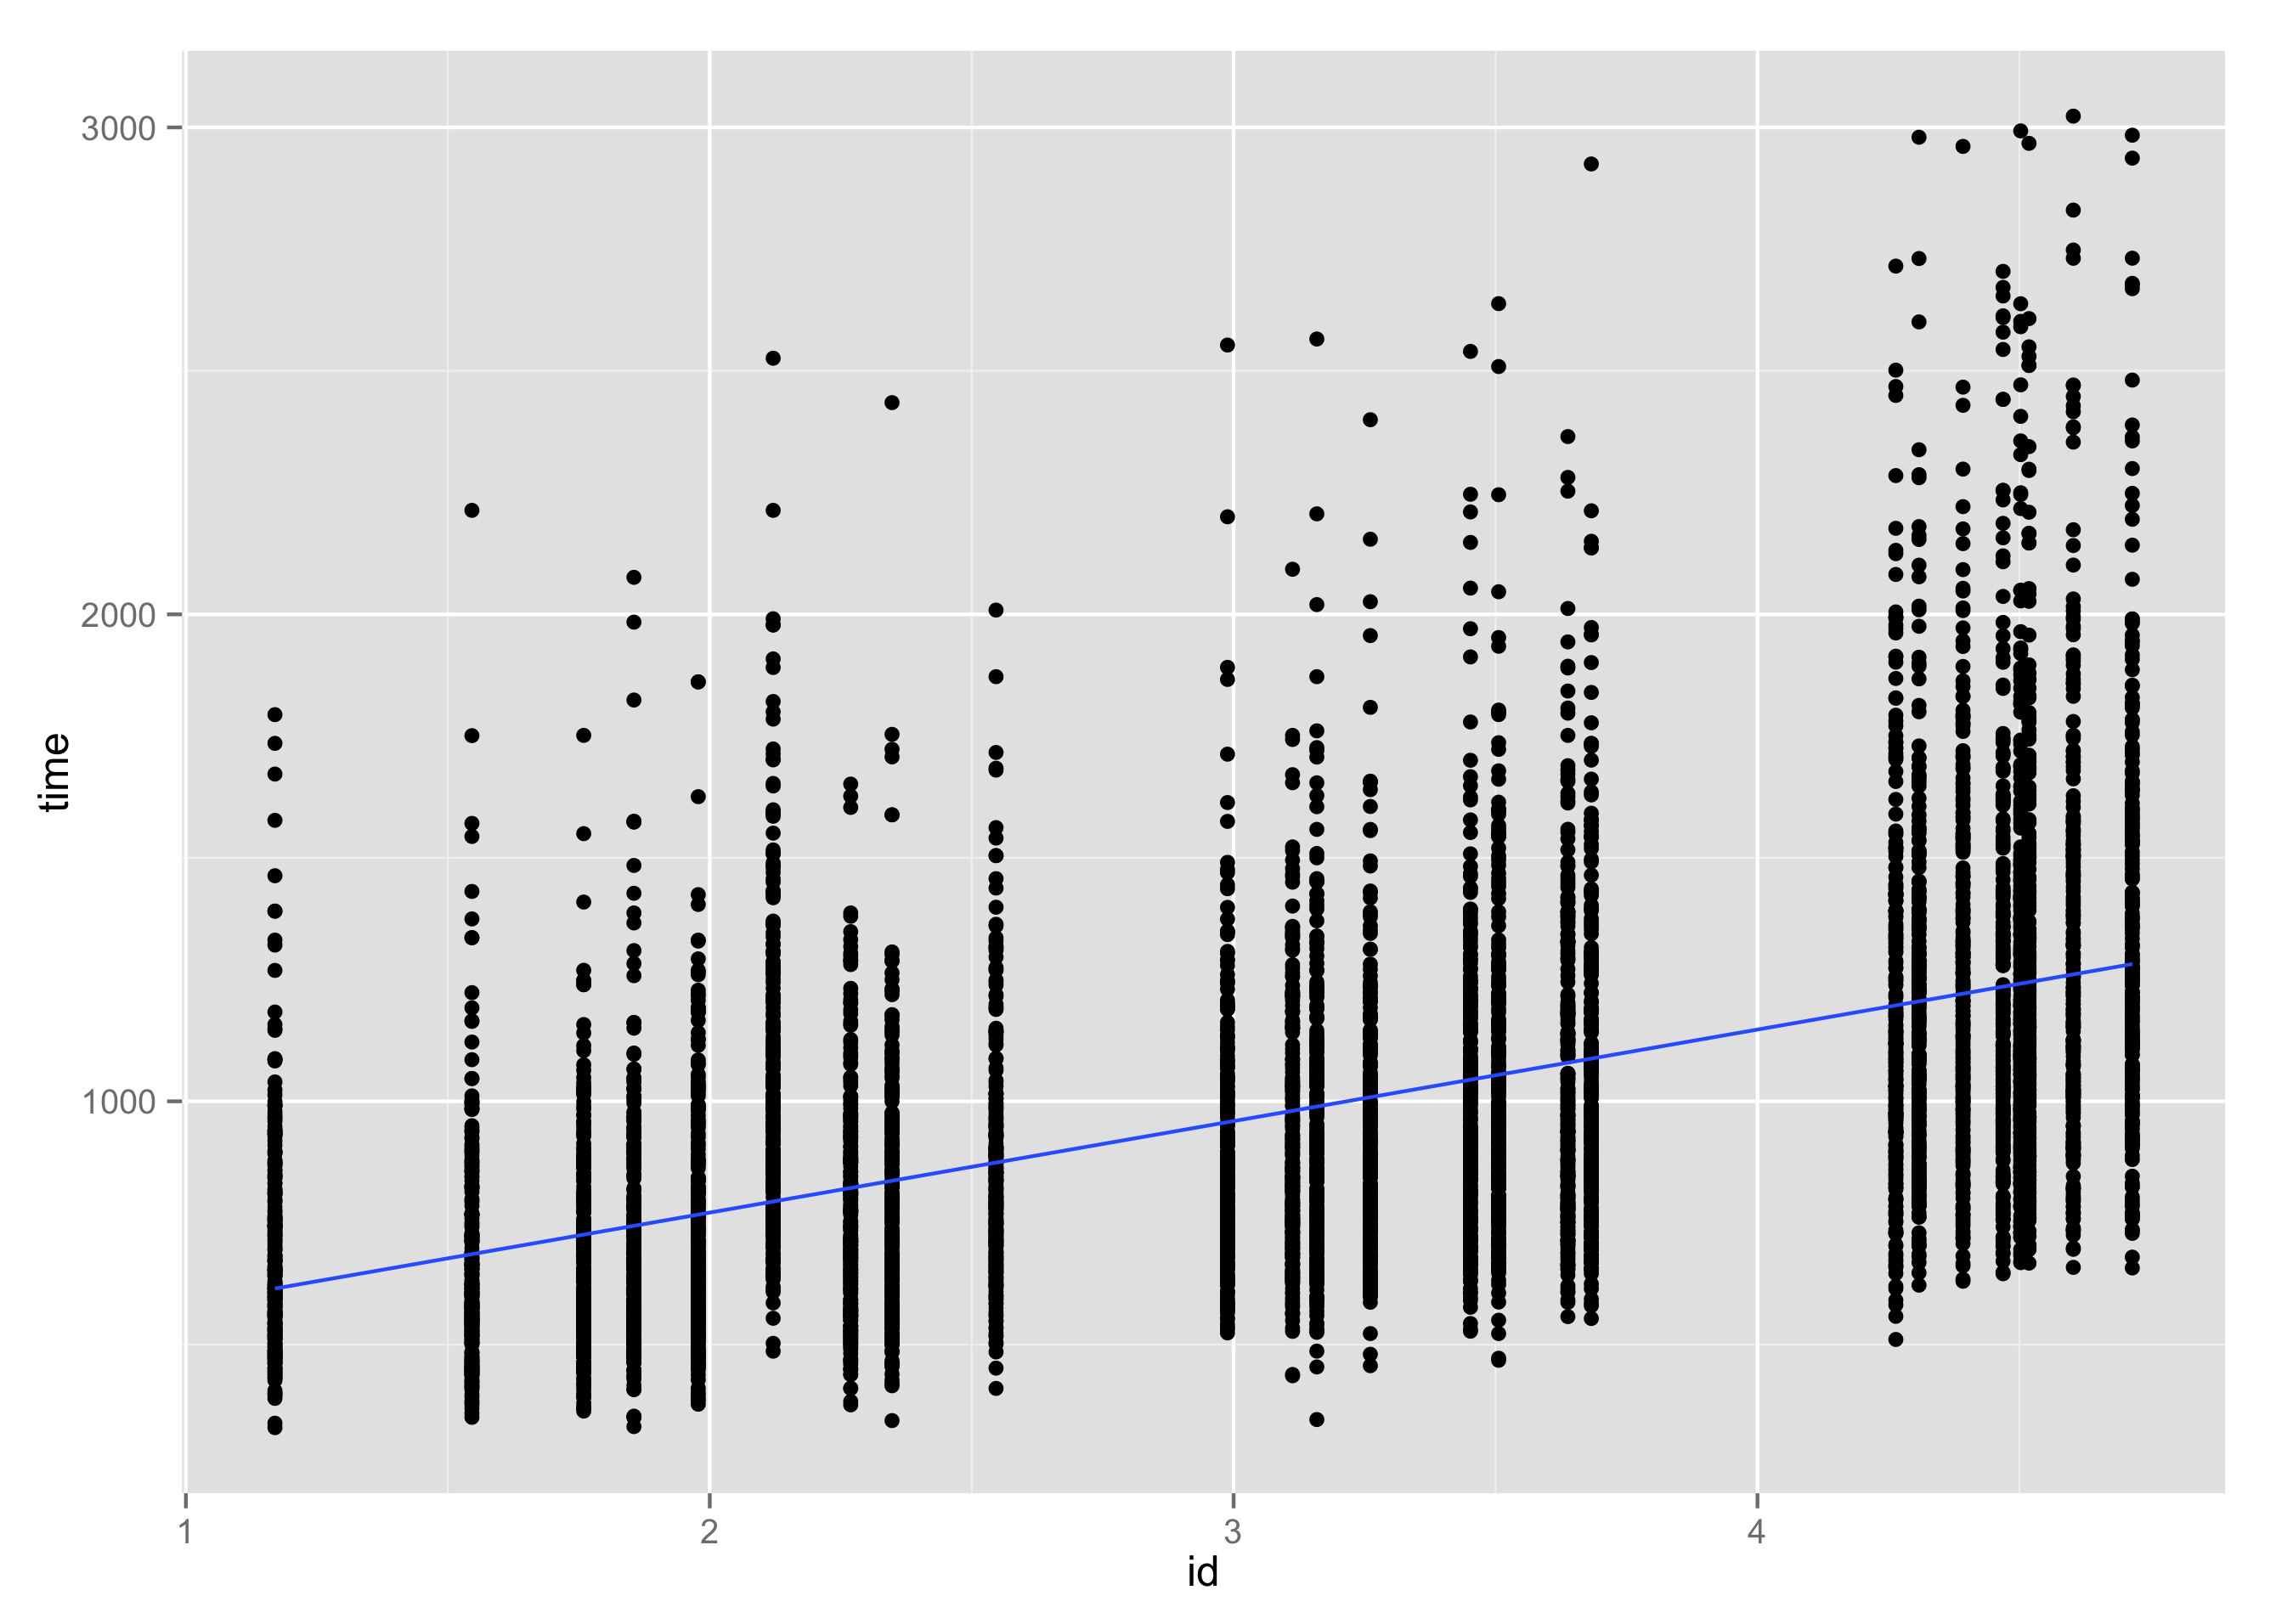
\includegraphics[width=\textwidth]{images/plots/plot_model_mackenzie}
		\captionof{figure}{Mackenzie's affine model med hans $ID$ ud af $x$-aksen og tiden ud af $y$-aksen}
		\label{fig:mackenzie_affine_line}
	\end{minipage}
\end{minipage}

\addcontentsline{toc}{subsection}{AIC-analyse}
\subsection*{AIC-analyse}
AIC-metoden anslår kvaliteten af hver model, relativt til hver af de andre modeller. Hvilket vil sige, at AIC-metoden ikke kan sige noget om kvaliteten af en model i absolut forstand, og derfor ikke kan vurdere hvor godt en model passer på dataene - kun den relative kvalitet af modellerne.

Tabel \ref{tab:table_analysis_aic1} viser AIC-værdier for de fire modeller tilpasset alle testdeltageres pegeopgaver, og den relative forskel imellem dem. Eftersom den absolute AIC-værdi ikke i sig selv siger noget, kigger vi kun på forskellen mellem dem. Tabel \ref{tab:table_analysis_aic2} viser AIC-værdier for alle pegeopgaver for 10 tilfældigt udvalgte personer, mens tabel \ref{tab:table_analysis_aic3} viser den relative forskel imellem de fire modellers AIC-værdier for de samme personer.

Den relative forskel mellem modellerne beskriver vi ved $\Delta_i$. Hvilket er beregnet som forskellen imellem AIC-værdien for den $i$'te model og AIC-værdien for modellen med den mindste AIC-værdi, se (\ref{eq:delta_aic}). Denne måde at beregne de relative forskelle er foreslået i \cite{burnham2004}.
\begin{align}
\Delta_i = AIC_i - AIC_{min}
\label{eq:delta_aic}
\end{align} 
De $\Delta$-værdier, som fremkommer af denne beregning vil være den information der mistes, ved at bruge en model fremfor en anden \cite{burnham2004}. Modeller med $\Delta_i \leq 2$ vil ikke kunne afskrives at kunne være lige så beskrivende som modellen med $AIC_{min}$, imens modeller med $\Delta_i > 10$ godt kan udelukkes fra fremtidige analyser af de pågældende data. Modeller med $4 \leq \Delta_i \leq 7$ kan ikke udelades, men kan heller ikke erstatte modellen med $AIC_{min}$ til fulde \cite{burnham2004}.

De indbyrdes forskelle i tabel \ref{tab:table_analysis_aic1} er alle over 10 og vi kan derfor beskrive Meyer's formulering, som den formulering, der beskriver vores data bedst. Forskellene for de 10 tilfældigt udvalgte personer, som ses i tabel \ref{tab:table_analysis_aic3}, ligger generelt lavere end forskellene i tabel \ref{tab:table_analysis_aic1}. For de fleste af personerne har Meyer's, MacKenzie's og Fitts' en forskel, som er mindre end eller lig med to, hvilket gør at de beskriver den indsamlede data lige godt. Forskellene for Welford's formulering er generelt højere, dog kun få over 10, hvilket gør, at vi ikke kan udelukke den som værende mere beskrivende for vores data, men, at den ikke beskriver vores data så præcist som de tre andre. 

\begin{table}[h]
\centering
\begin{tabular}{lll}
Model 	  & AIC-værdi & Forskel\\\hline
Meyer 	  & 92728.38 & 0 \\
Mackenzie & 92763.02 & 34.64 \\
Fitts 	  & 92804.17 & 75.79 \\
Welford   & 94510.34 & 1781.96
\end{tabular}
\caption{AIC-værdier for alle personers pegeopgaver og indbyrdes forskel med udgangspunkt i Meyer's som nulpunkt}
\label{tab:table_analysis_aic1}
\end{table}

\begin{table}[h]
\centering
\begin{tabular}{lllll}
Person & Meyer  & MacKenzie & Fitts  & Welford \\\hline
107    & 353.94 & 355.67    & 356.61 & 357.17  \\
108    & 338.06 & 339.06    & 339.56 & 351.69  \\
56     & 357.82 & 358.15    & 358.42 & 359.68  \\
246    & 357.16 & 357.35    & 357.56 & 366.10  \\
68     & 343.20 & 344.42    & 344.86 & 352.58  \\
140    & 325.15 & 325.07    & 325.12 & 350.23  \\
25     & 330.44 & 333.60    & 334.84 & 335.92  \\
164    & 349.84 & 351.44    & 352.02 & 354.79  \\
255    & 355.91 & 356.39    & 356.76 & 355.85  \\
59     & 360.84 & 360.66    & 360.79 & 365.70
\end{tabular}
\caption{AIC-værdier for alle pegeopgaver for 10 tilfældigt udvalgte personer}
\label{tab:table_analysis_aic2}
\end{table}

\begin{table}[h]
\centering
\begin{tabular}{lllll}
Person & Meyer  & MacKenzie & Fitts  & Welford \\\hline
107    & 0      & 1.72      & 2.67   & 3.23    \\
108    & 0      & 1.00      & 1.50   & 13.63   \\
56     & 0      & 0.33      & 0.60   & 1.86    \\
246    & 0      & 0.19      & 0.40   & 8,94    \\
68     & 0      & 1.22      & 1.66   & 9.38    \\
140    & 0.08   & 0         & 0.05   & 25.16   \\
25     & 0      & 3.16      & 4.40   & 5.48    \\
164    & 0      & 1.60      & 2.18   & 4.95    \\
255    & 0.06   & 0.54      & 0.91   & 0       \\
59     & 0.18   & 0         & 0.13   & 5.04
\end{tabular}
\caption{Indbyrdes forskel mellem AIC-værdierne for 10 tilfældigt udvalgte personer. Forskellen er udregnet med udgangspunkt i modellen med lavest AIC-værdi}
\label{tab:table_analysis_aic3}
\end{table}

\addcontentsline{toc}{subsection}{Residualanalyse}
\subsection*{Residualanalyse}
For at få en ekstra vurdering af præcisionen af modellerne, har vi valgt at lave en residualanalyse. Residualerne i modellerne er variationen i $ID$ som modellerne ikke opfanger, og de kan derved sige noget om, hvor præcis modellerne er i forhold til den data vi har indsamlet.

På figur \ref{fig:plot_residual_fitt}, \ref{fig:plot_residual_welford}. \ref{fig:plot_residual_mackenzie} og \ref{fig:plot_residual_meyer} ses alle fire modellers residualplot, med en blå linje defineret af en smoothing-funktion. Smoothing-funktionen er tilføjet som et visuelt hjælpemiddel der tydeligt kan vise hvordan residualerne fordeler sig omkring x-aksen. Jo mere centreret de er om aksen, og jo mere linære de er i forhold til aksen, jo bedre er modellen. Smoothing-funktionen har vi ikke kunne finde præcis dokumentation for, men vi formoder, at den tegner en linje mellem beregnede gennemsnit for $y$-koordinaterne til hver $x$-koordinat, med negative værdier under den røde linje og positive over.

Når vi kigger på de fire residualplot, så viser de samme resultater som AIC-analysen. Welford's residualplot viser, at modellen passer dårligt på den indsamlede data. Fitt's og MacKenzie's ligner hinanden meget, mens Meyer's er den model der giver det bedste fit til den indsamlede data.

Det ses af figur \ref{fig:plot_residual_welford}, at Welford's især er dårligere ved lavere værdier af $ID$. Grunden til dette er, at Welford's ikke har det additive $a$-led. Som Welford \cite{welford1968} selv forklarer, så vil det manglende $a$-led ikke gøre stor forskel ved større værdier af $ID$. Fitt's og MacKenzie's residualer ligner hinanden.

\begin{minipage}{\linewidth}
	\begin{minipage}{.5\linewidth}
		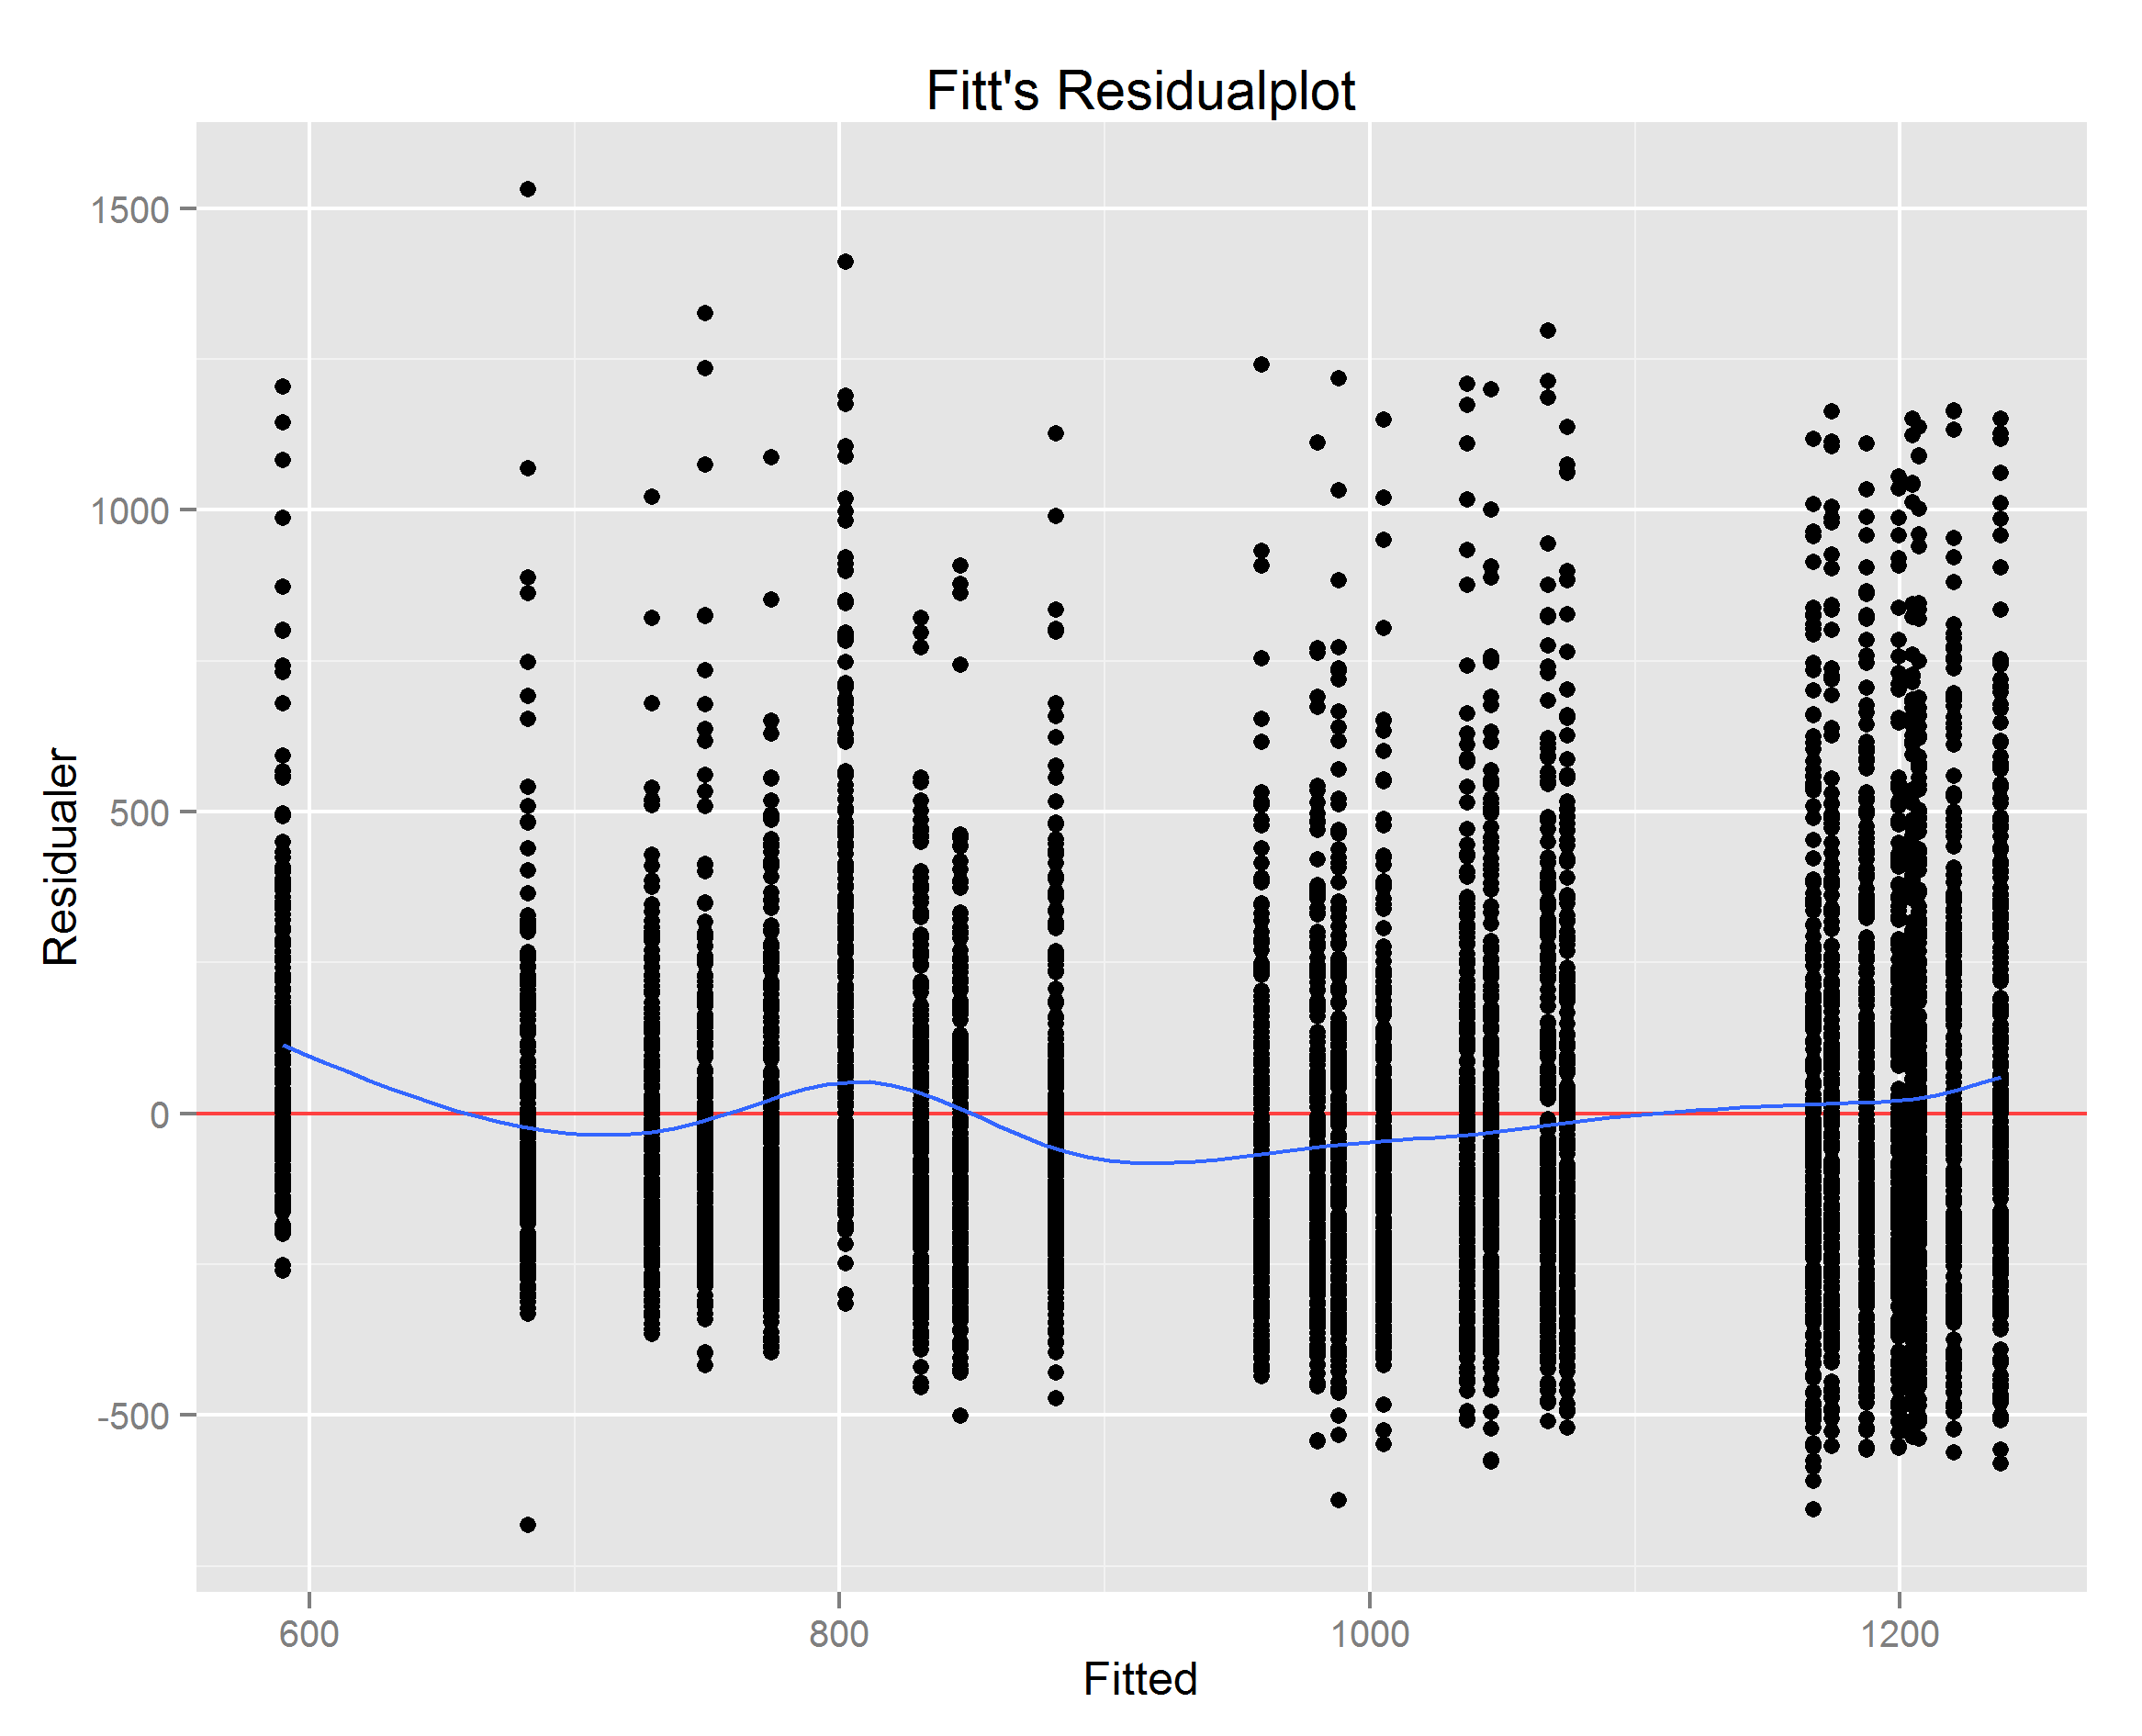
\includegraphics[width=\linewidth]{images/plots/plot_residual_fitt}
		\captionof{figure}{Fitts' residualplot}
		\label{fig:plot_residual_fitt}
	\end{minipage}
	\begin{minipage}{.5\linewidth}
		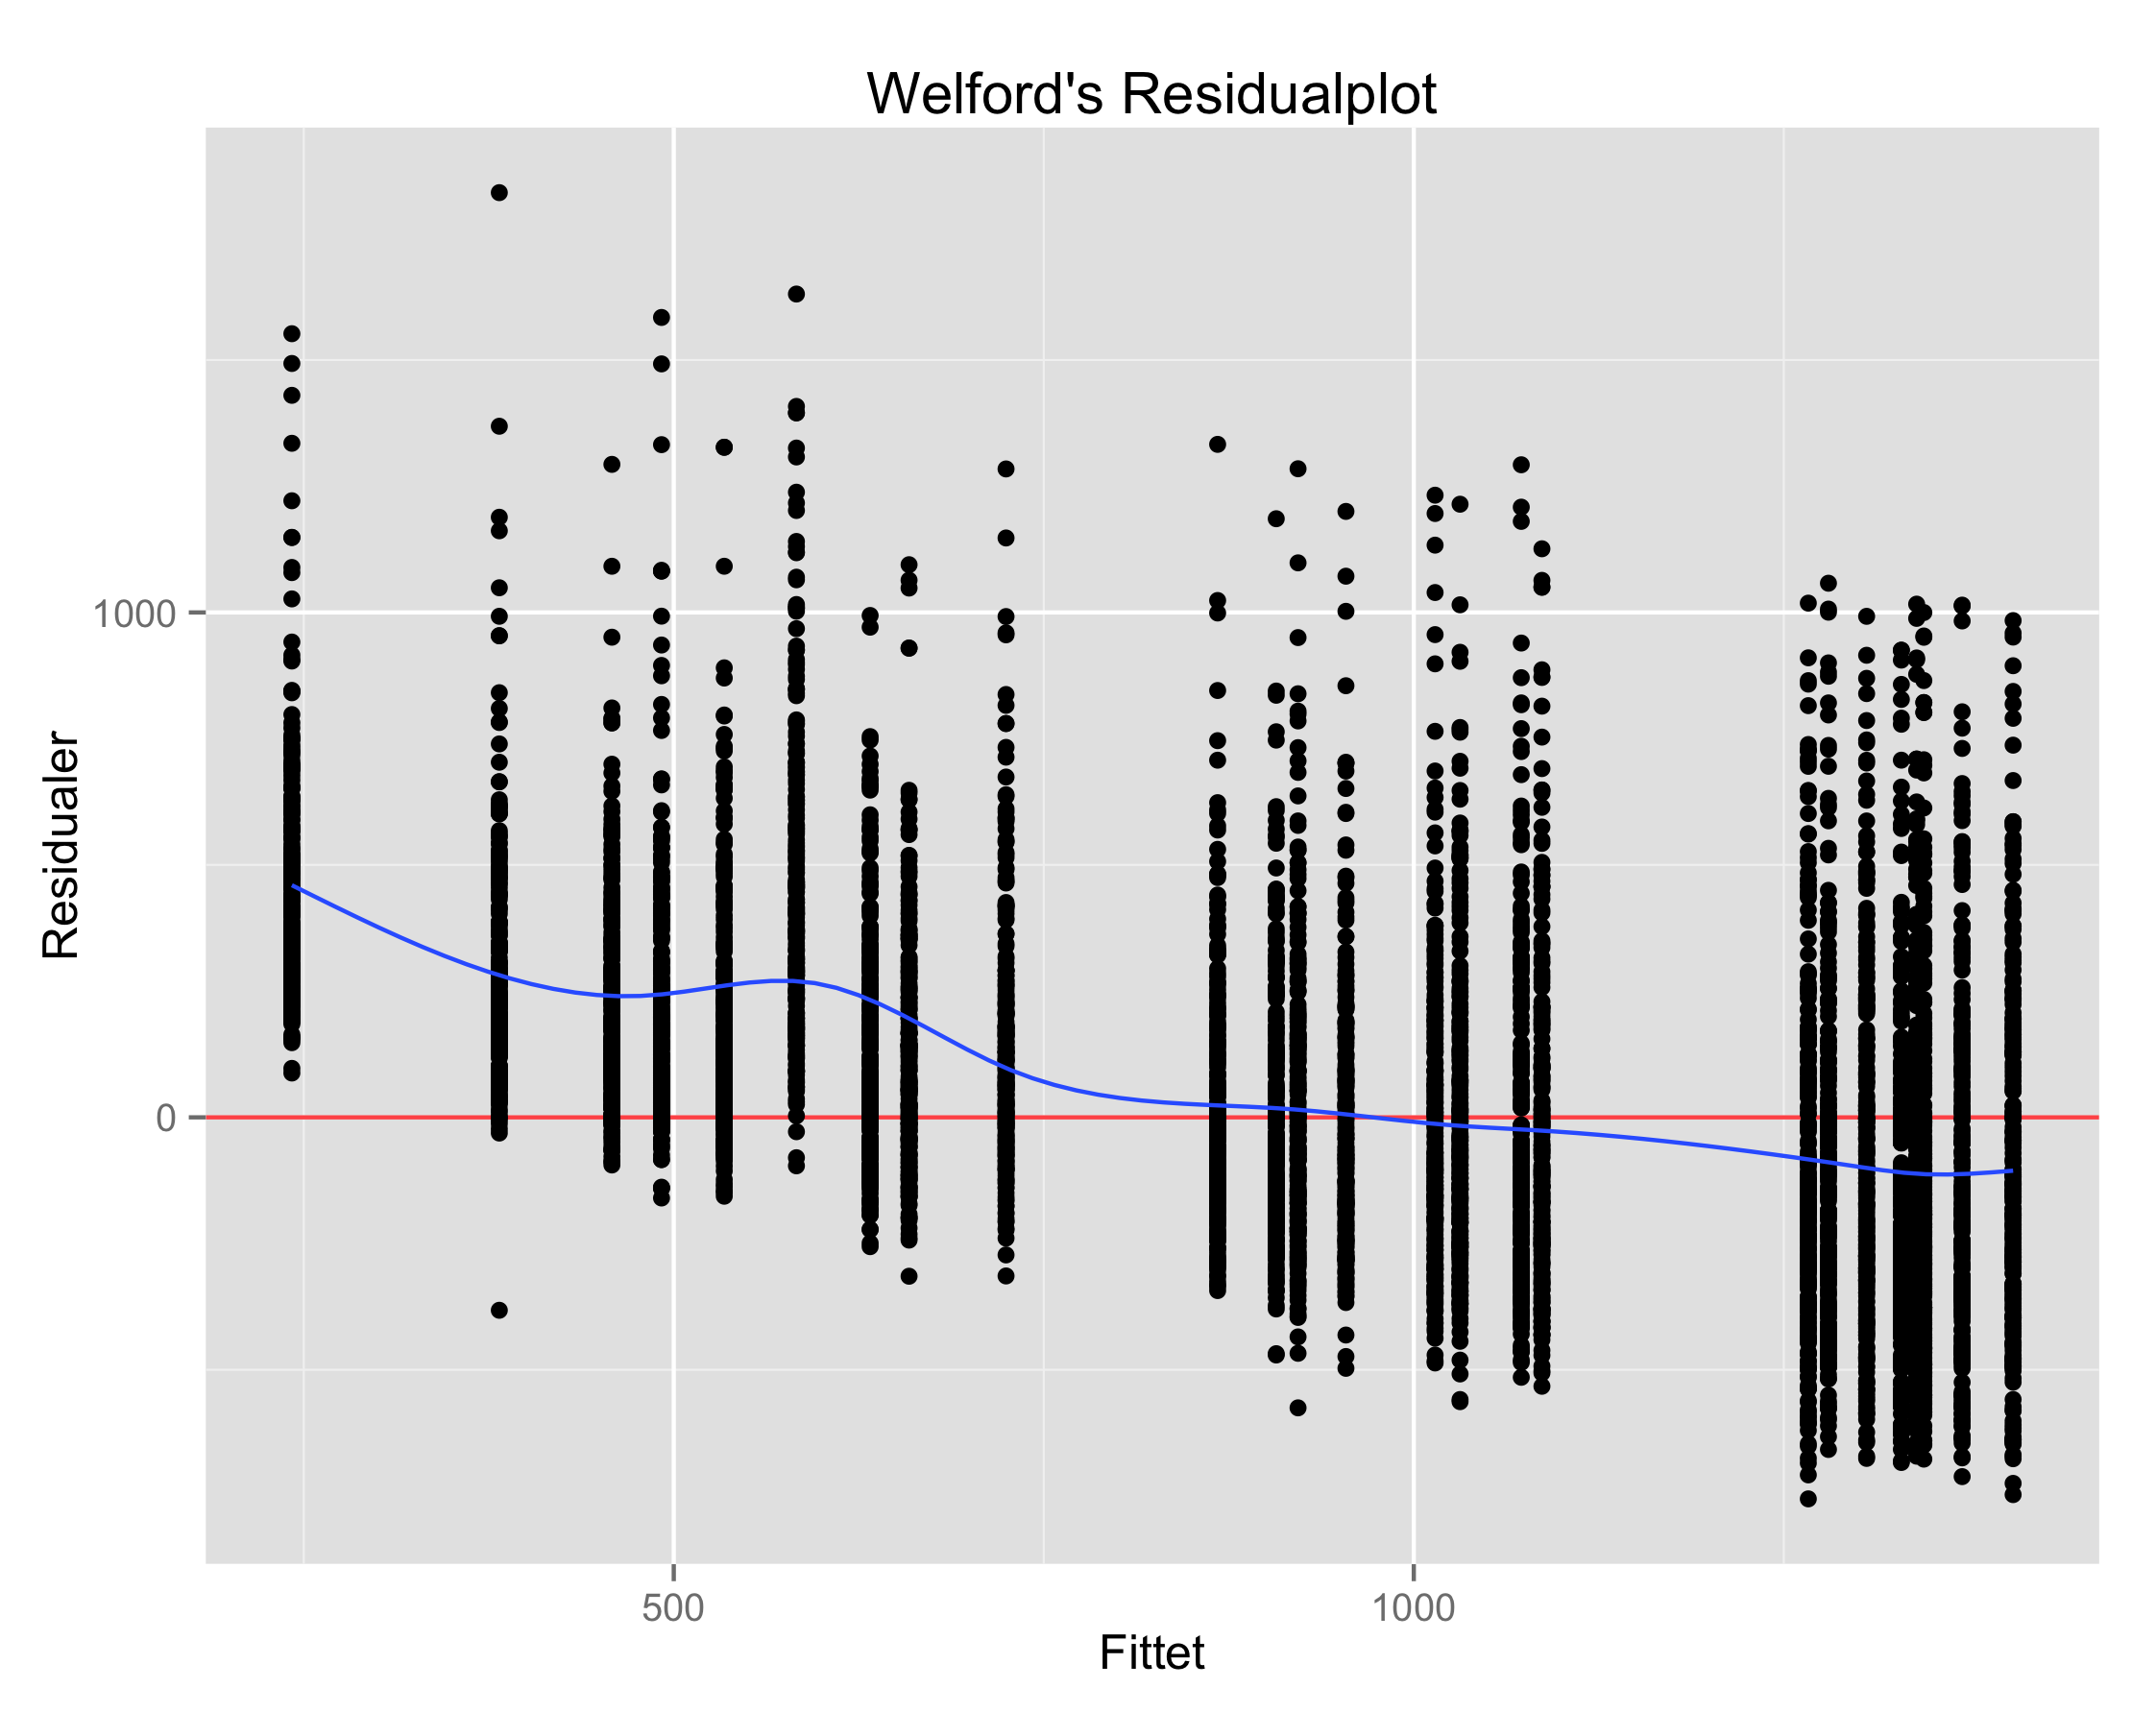
\includegraphics[width=\linewidth]{images/plots/plot_residual_welford}
		\captionof{figure}{Welford's residualplot}
		\label{fig:plot_residual_welford}
	\end{minipage}
	\begin{minipage}{.5\linewidth}
		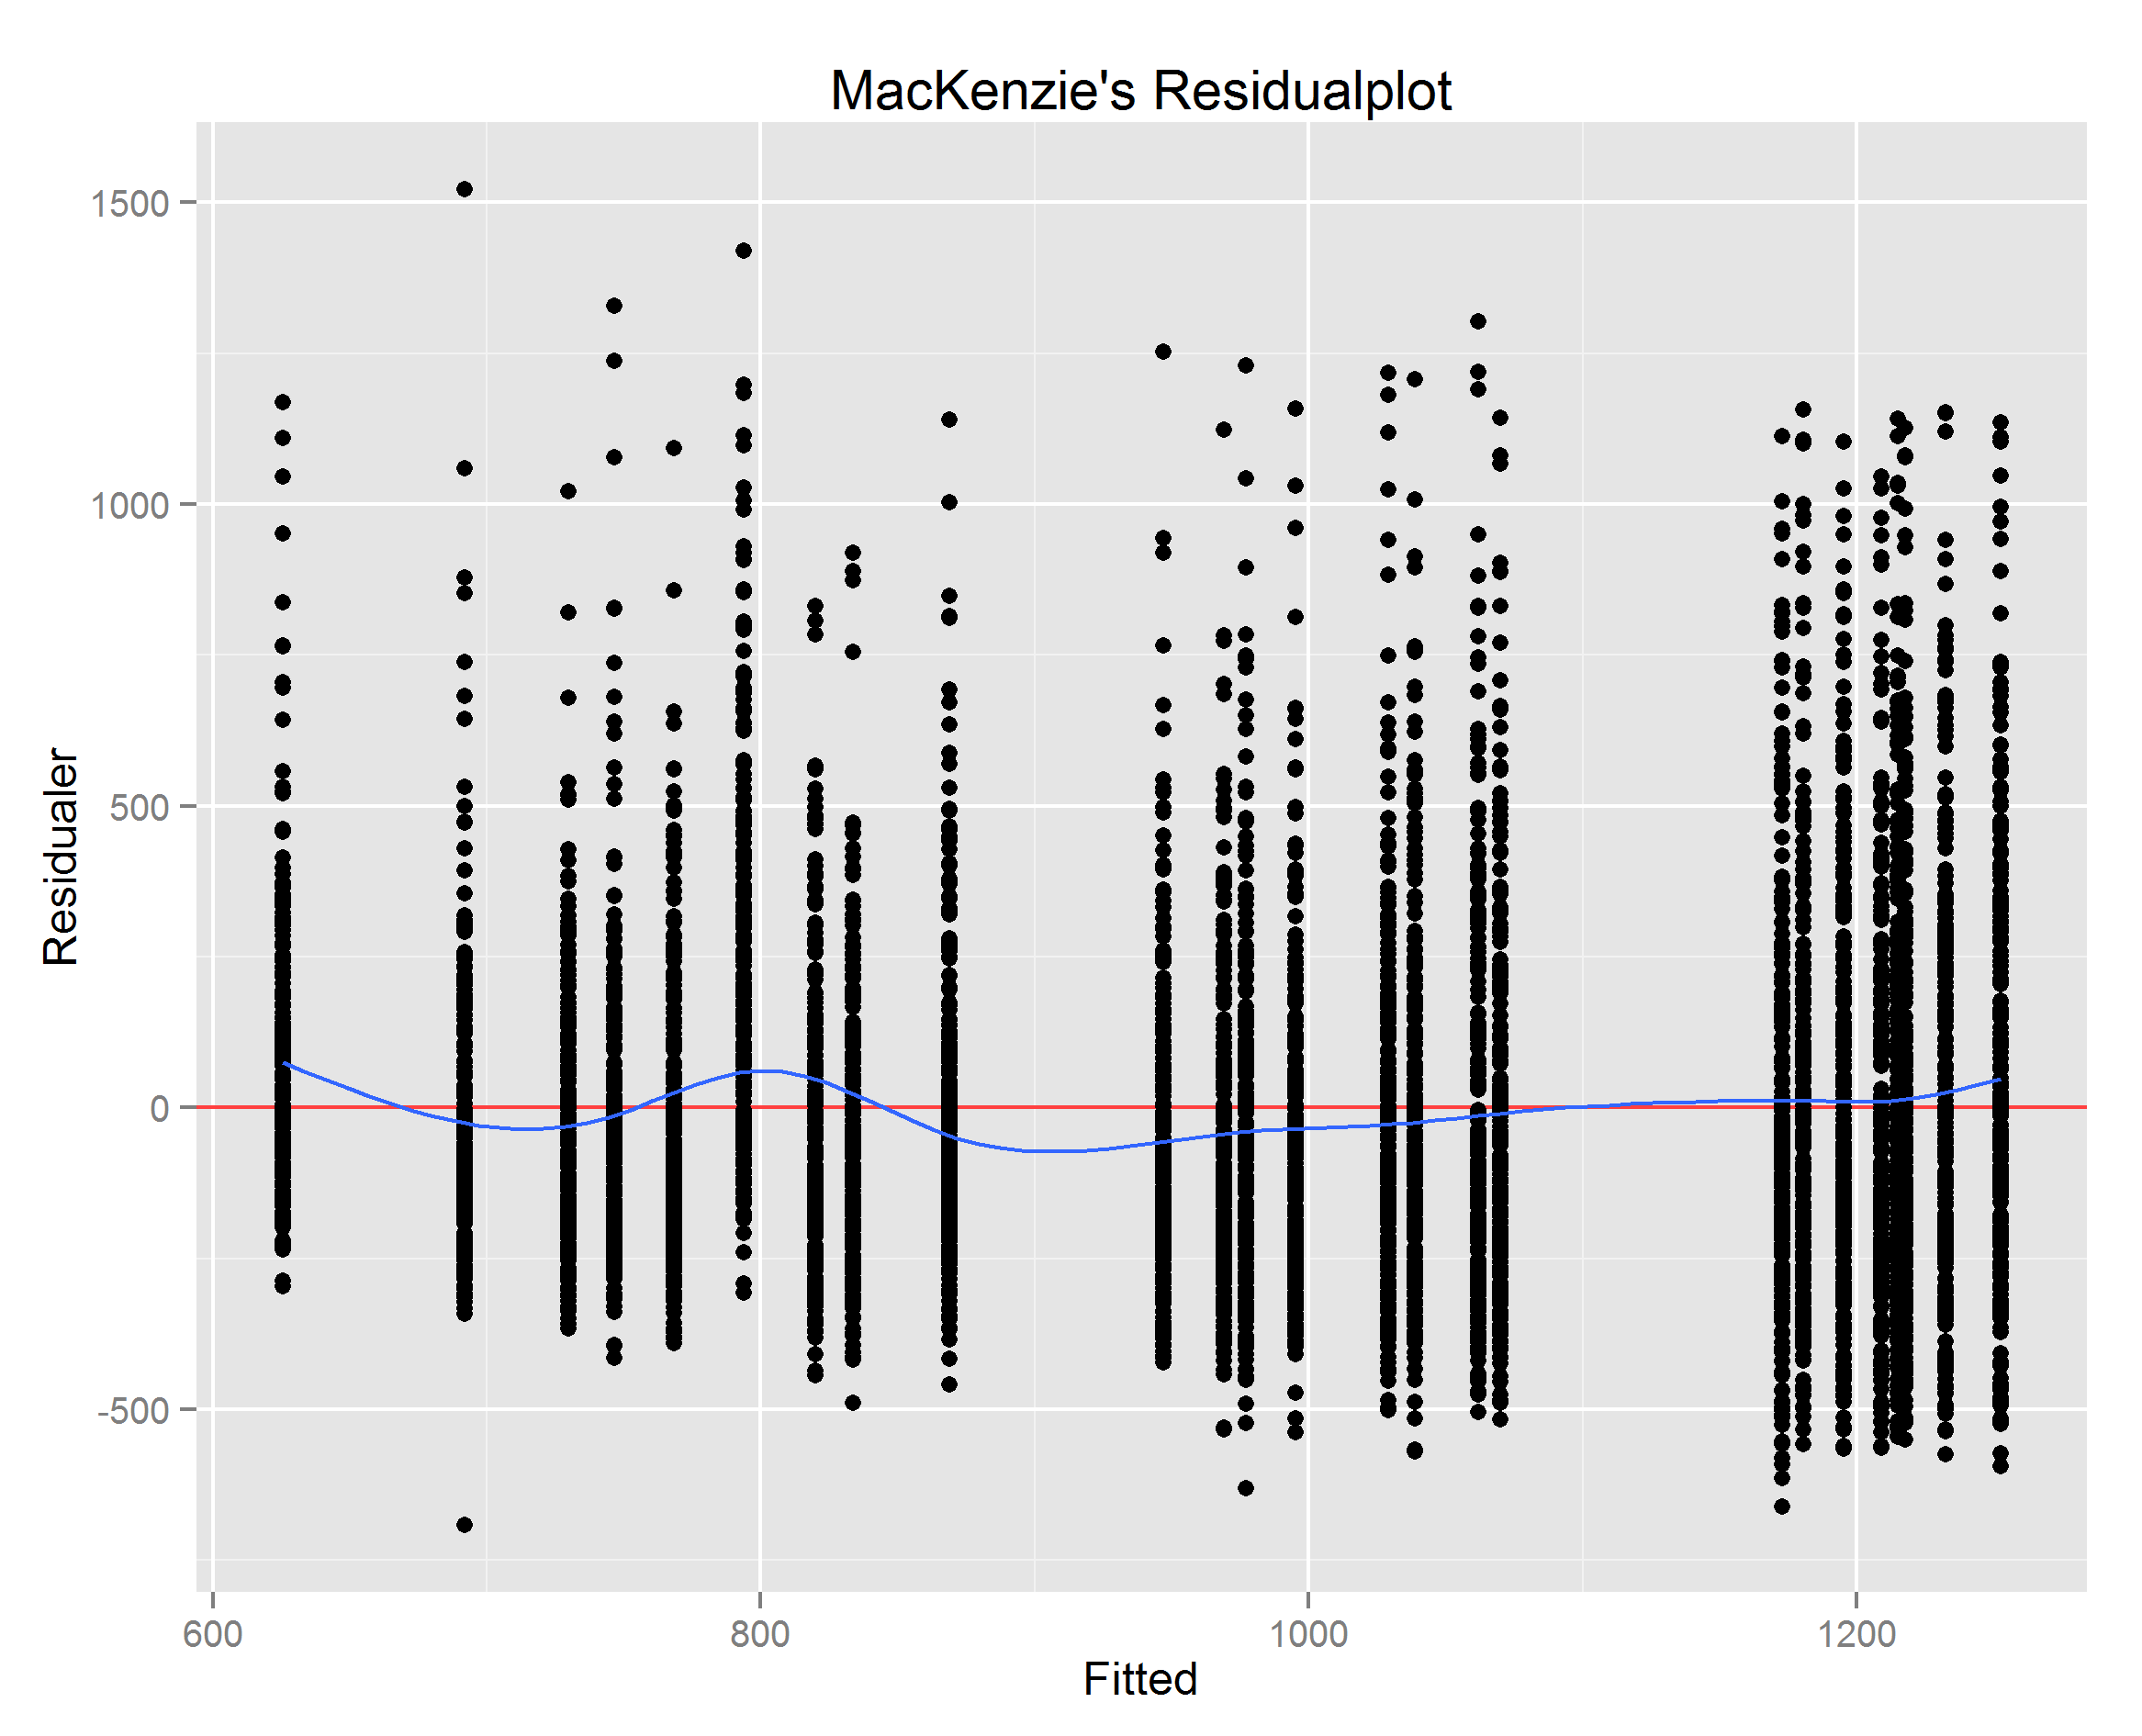
\includegraphics[width=\linewidth]{images/plots/plot_residual_mackenzie}
		\captionof{figure}{MacKenzie's residualplot}
		\label{fig:plot_residual_mackenzie}
	\end{minipage}
	\begin{minipage}{.5\linewidth}
		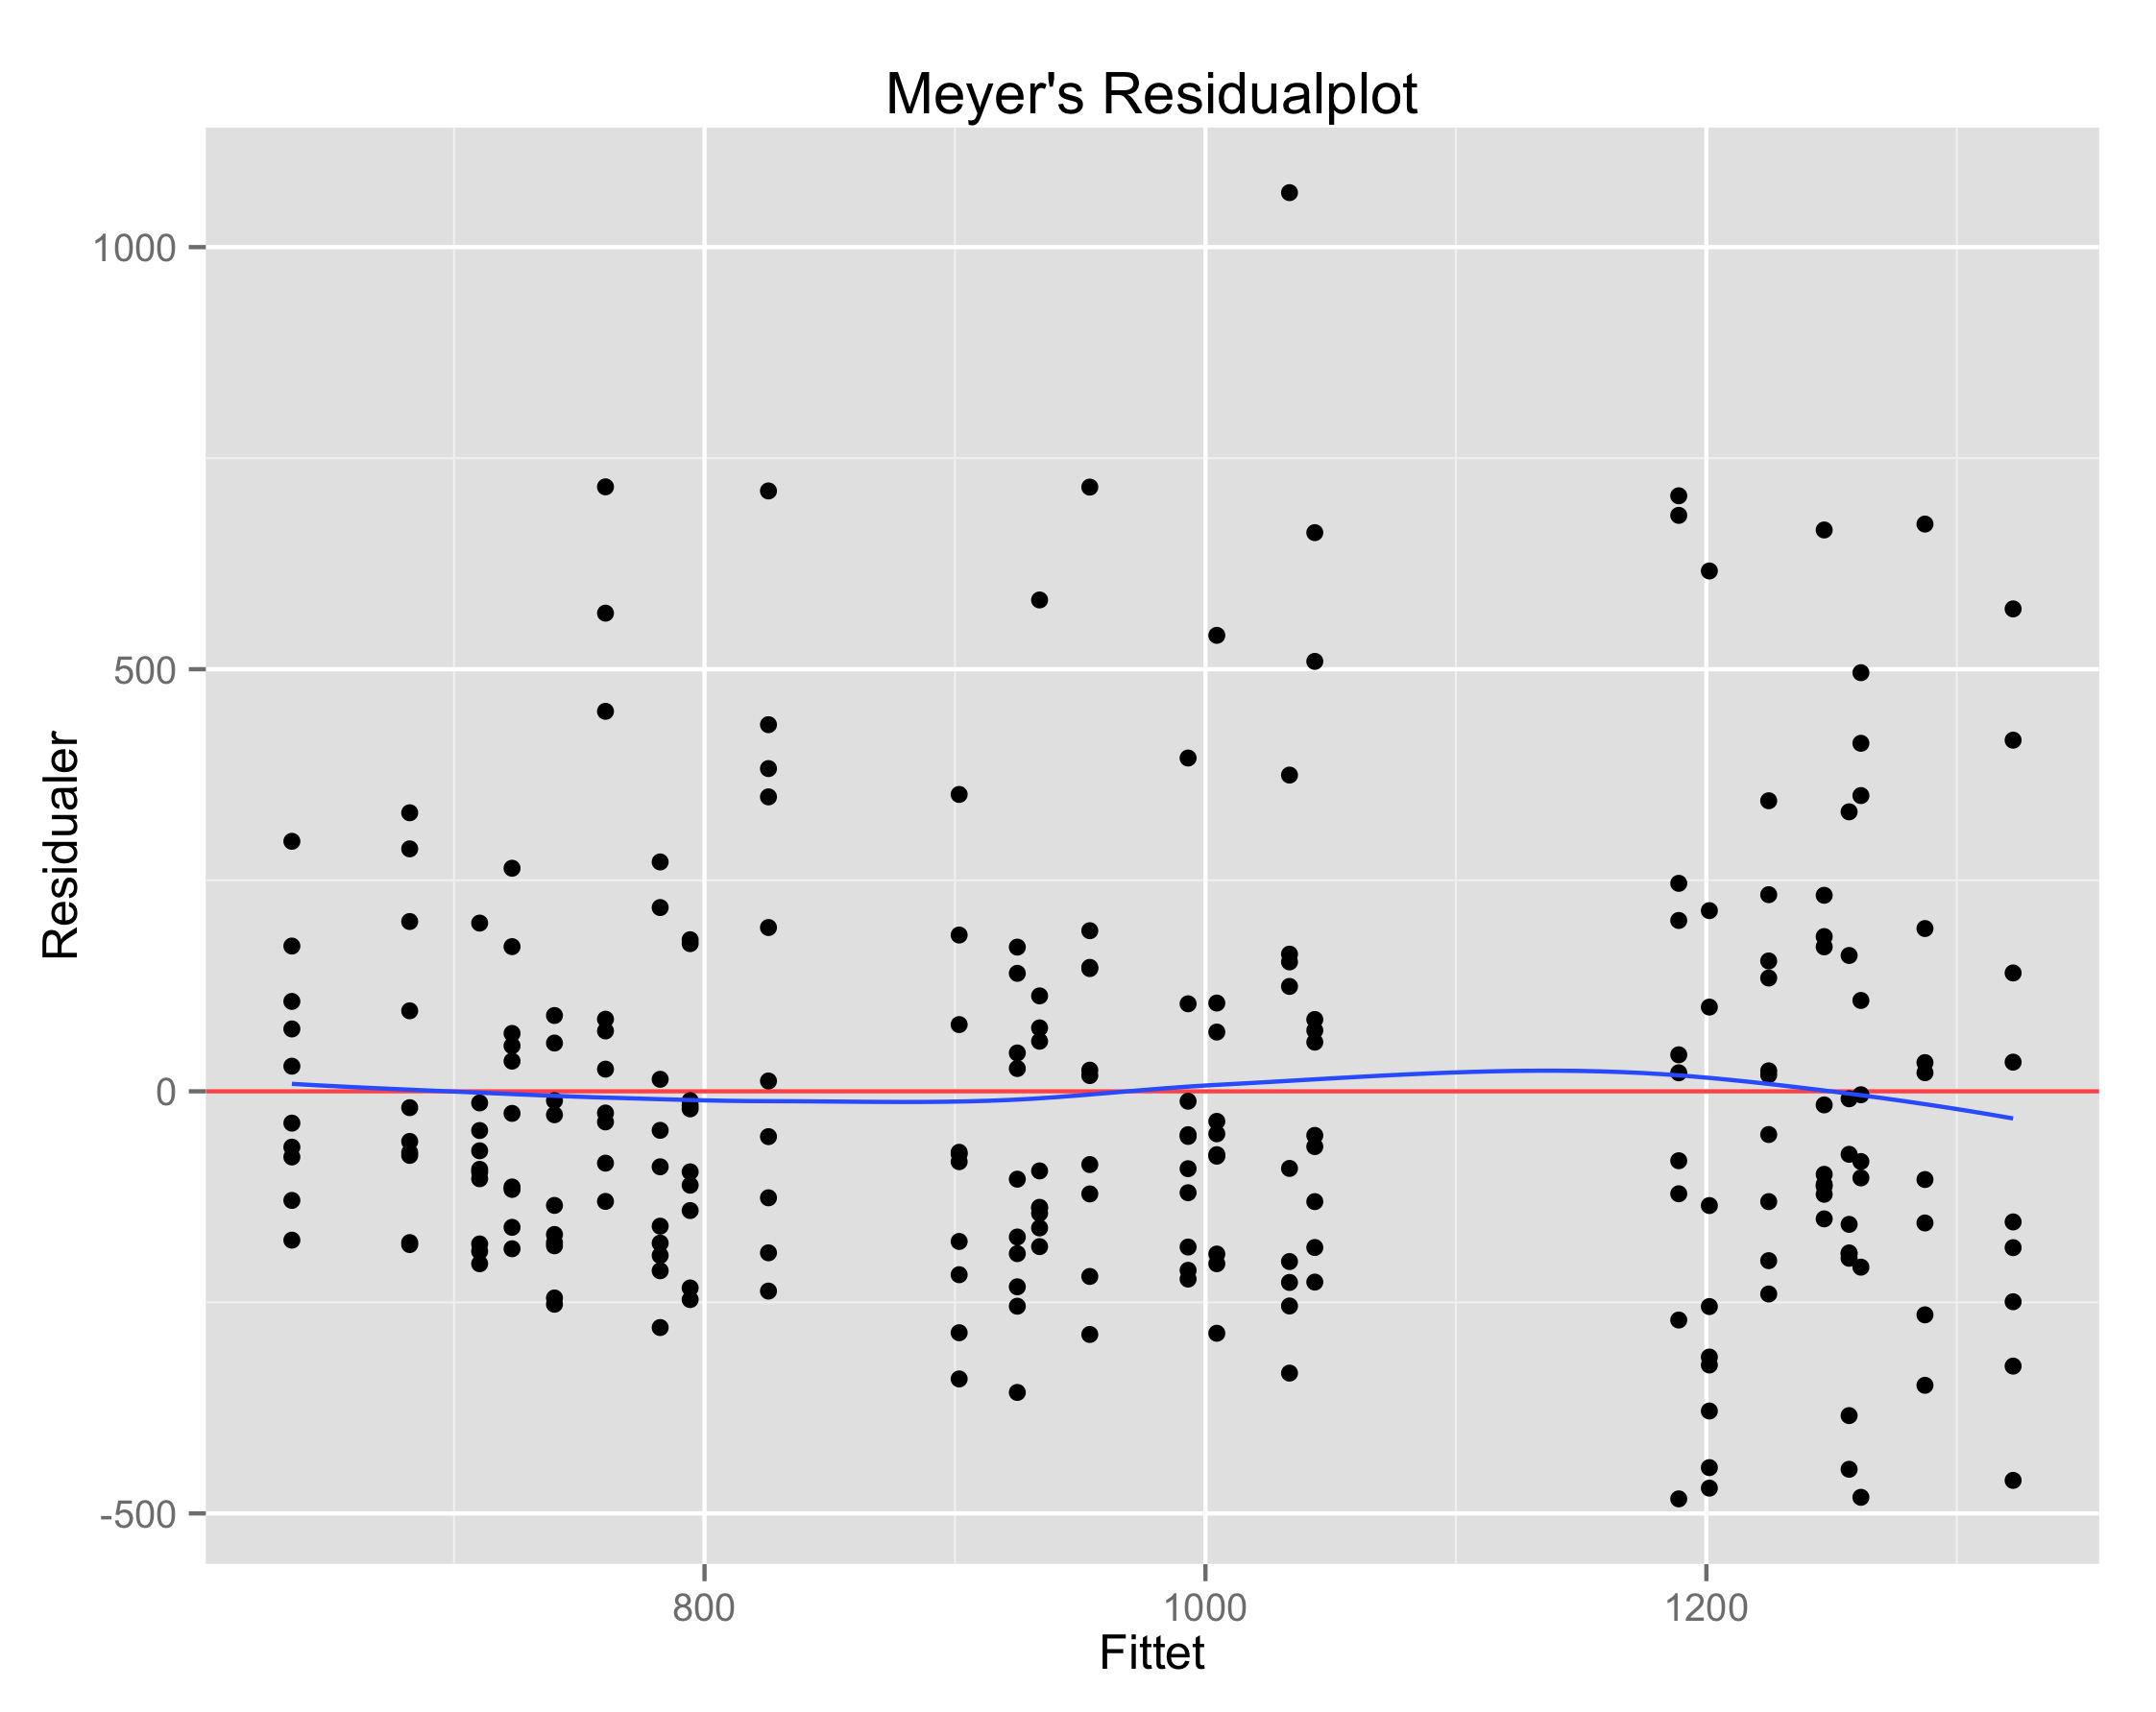
\includegraphics[width=\linewidth]{images/plots/plot_residual_meyer}
		\captionof{figure}{Meyer's residualplot}
		\label{fig:plot_residual_meyer}
	\end{minipage}
\end{minipage}

\addcontentsline{toc}{section}{Modelanalyse af navigationsopgaver}
\section*{Modelanalyse af navigationsopgaver}
I vores forsøg havde vi, udover pegeopgaven, også tunnel- og spiralopgaver. Vi vil i dette afsnit forsøge at tilpasse de fire formuleringer af Fitts' lov til data fra vores navigationsopgaver, velvidende, at det ikke er en type af opgaver de er beregnet til. Accot og Zhai har undersøgt lignende navigationsopgaver og fundet et $ID$ specifikt for både tunnel- og spiralopgaver, hvilket vi vil bruge til at sammenligne med de fire formuleringer \cite{accot1997}.

\addcontentsline{toc}{subsection}{Analyse af tunnelopgaver}
\subsection*{Analyse af tunnelopgaver}
De fire formuleringer er, som benævnt, ikke lavet til navigationsopgaver. Vi har dog alligevel tilpasset en affin model med deres respektive $ID$, til vores 264 testdeltageres tunnelopgaver. Vi har valgt afstanden, $A$, til at være længden på tunnellen, $A=[20,30,40,50]$, målt i pixels. Bredden, $W$, har vi valgt som størrelsen på tunnelens højre lodrette linje, slutstregen, der altid er $8$ pixels. Ved lineær regression, fik vi tilpasset nedenstående matematiske modeller af de fire formuleringer.

\begin{align*}
\text{Fitts': } &T = 3532.2 + 581.9\cdot \log_2\left(\frac{2A}{W}\right)\\
\text{Welford's: } &T =  1242.58\cdot \log_2\left(\frac{A+\frac{1}{2}W}{W}\right)\\
\text{MacKenzie's: } &T = 4036.7 + 592.3\cdot \log_2\left(\frac{A+W}{W}\right)\\
\text{Meyer's: } &T = 5863.07 + 210.48 \cdot \sqrt{\frac{A}{W}}
\end{align*}

Det additive led er markant højere for tunnelopgaverne end for pegeopgaverne, da det gennemsnitligt har taget længere tid for vores testdeltagere at gennemføre dem. Gennemsnitstiden for de 264 testdeltageres tunnelopgaver er $7673.01$ millisekunder imod $983.30$ millisekunder for pegeopgaverne. Det additive led kan dog ikke tolkes som reaktionstiden for tunnelopgaverne. Dette skyldes, at tiden bliver registreret fra, testdeltageren passerer startstregen i tunnellen, og derved allerede er i bevægelse ved $T=0$.

Accot og Zhai beskriver i deres artikel \cite{accot1997}, hvordan en indsnævrende tunnelopgave kan opdeles i små delelementer, som hver især udgør én lille navigationsopgave. Ved at gøre dette kan man finde $ID$ som summen af delelementernes $ID$, hvilket resulterer i 
\begin{align*}
ID_{NT} = \frac{A}{W_2-W_1}\ln\left(\frac{W_2}{W_1}\right)
\end{align*}
$W_1$ er størrelsen på startstregen, og $W_2$ er størrelsen på slutstregen, imens $A$ er længden af tunnelen. I følge Accot og Zhai er der en affin sammenhæng imellem tiden $T$ og dette $ID_{NT}$, hvilket giver anledning til følgende formulering $T = a+b\cdot ID_{NT}$. Tilpasses denne formulering med lineær regression til vores 264 testdeltageres tunnelopgaver findes nedenstående matematiske model.

\begin{align*}
\text{Accot \& Zhai: } T = 6112.40+47.77 \cdot \left(\frac{A}{W_2-W_1}\cdot\ln\left(\frac{W_2}{W_1 }\right)\right)
\end{align*}

Det kan bemærkes, at den primære forskel imellem Accot og Zhai's formulering og de fire andre er det multiplikative led, $b$. Da $ID_{NT}$ antager væsentligt højere værdier end de fire andre $ID$'er, så er $b$ også tilsvarende mindre. For at visualisere de fem formuleringers tilpasning til dataene har vi beregnet gennemsnitstiden for alle testdeltagerne per $ID$. Dette giver anledning til fire datapunkter, ét for hver tunnelopgave, som kan ses i figur \ref{fig:welford_tunnel_line}, \ref{fig:fitt_tunnel_line}, \ref{fig:meyer_tunnel_line}, \ref{fig:mackenzie_tunnel_line} og \ref{fig:accot_tunnel_line} sammen med de tilpassede affine kurver. På $x$-aksen er modellernes respektive $ID$ imens tiden, $T$ er angivet ved $y$-aksen. 

Af graferne ser det ud til, at Welford's formulering er markant dårligere til at beskrive vores data end de fire andre formuleringer. For at undersøge dette har vi lavet AIC-analyse af formuleringerne tilpasset det fulde datasæt, vist i tabel \ref{tab:table_analysis_aic_tunnel_all}, og gennemsnitsdatapunkterne, vist i tabel \ref{tab:table_analysis_aic_tunnel_mean}. Begge tabeller viser en klar tendens i og med, at Meyer's formulering er bedst til at beskrive vores data imens Welford's er dårligst. Begge tabeller viser den samme rækkefølge for formuleringernes indbyrdes placering, men de relative forskelle varierer.\\\\
\begin{minipage}[t]{\linewidth} 
	\begin{minipage}[t]{0.45\linewidth}
			\begin{tabular}{lll}
				Model & AIC-værdi & Forskel\\\hline
				Meyer & 20549.61 & 0 \\
				Accot \& Zhai & 20549.62 & 0.01\\
				MacKenzie & 20549.68 & 0.07 \\
				Fitts & 20549.68 & 0.07\\
				Welford & 20558.46 & 8.84
			\end{tabular}
			\captionof{table}{AIC-værdier for de 264 testdeltageres tunnelopgaver. Deres indbyrdes forskel er beregnet med udgangspunkt i Meyer's formulering som nulpunkt}
			\label{tab:table_analysis_aic_tunnel_all}
	\end{minipage}
	\begin{minipage}[t]{0.1\linewidth}
	~
	\end{minipage}
	\begin{minipage}[t]{0.45\linewidth}
			\begin{tabular}{lll}
				Model & AIC-værdi & Forskel\\\hline
				Meyer & 33.68 & 0 \\
				Accot \& Zhai & 38.17 & 4.49\\
				MacKenzie & 46.58 & 12.9 \\
				Fitts & 46.87 & 13.19\\
				Welford & 64.97 & 31.29
			\end{tabular}
			\captionof{table}{AIC-værdier for gennemsnittet af tiderne for de 264 testdeltageres tunnelopgaver ved hvert $ID$. Deres indbyrdes forskel er beregnet med udgangspunkt i Meyer's formulering som nulpunkt}
			\label{tab:table_analysis_aic_tunnel_mean}
	\end{minipage}
\end{minipage}\\\\
Selvom Accot og Zhai's formulering er specificeret til denne type opgaver, er det ikke den, som beskriver vores data bedst. Dette kan være på grund af, at vi kun har fire tunnelopgaver. Endvidere kan det være på grund af store forskelle i vores testdeltageres løsninger af opgaverne. Hvis vi tilpasser Accot og Zhai's formulering til vores kontrollerede testpersoners individuelle data, så kan det visualiseres, hvor stor afvigelse der er imellem testdeltagerne. Figur \ref{fig:navigationtest1} viser den traditionelle stigning i tiden med tilsvarende stigning i $ID$, men på figur \ref{fig:navigationtest2} kan det ses, hvordan datapunkterne opfører sig stik modsat. Det vil sige, at testperson 9 var hurtigere til at klare opgaverne i takt med, at de blev sværere.\\\\
\begin{minipage}{\linewidth}
	\begin{minipage}[b]{.45\linewidth}
		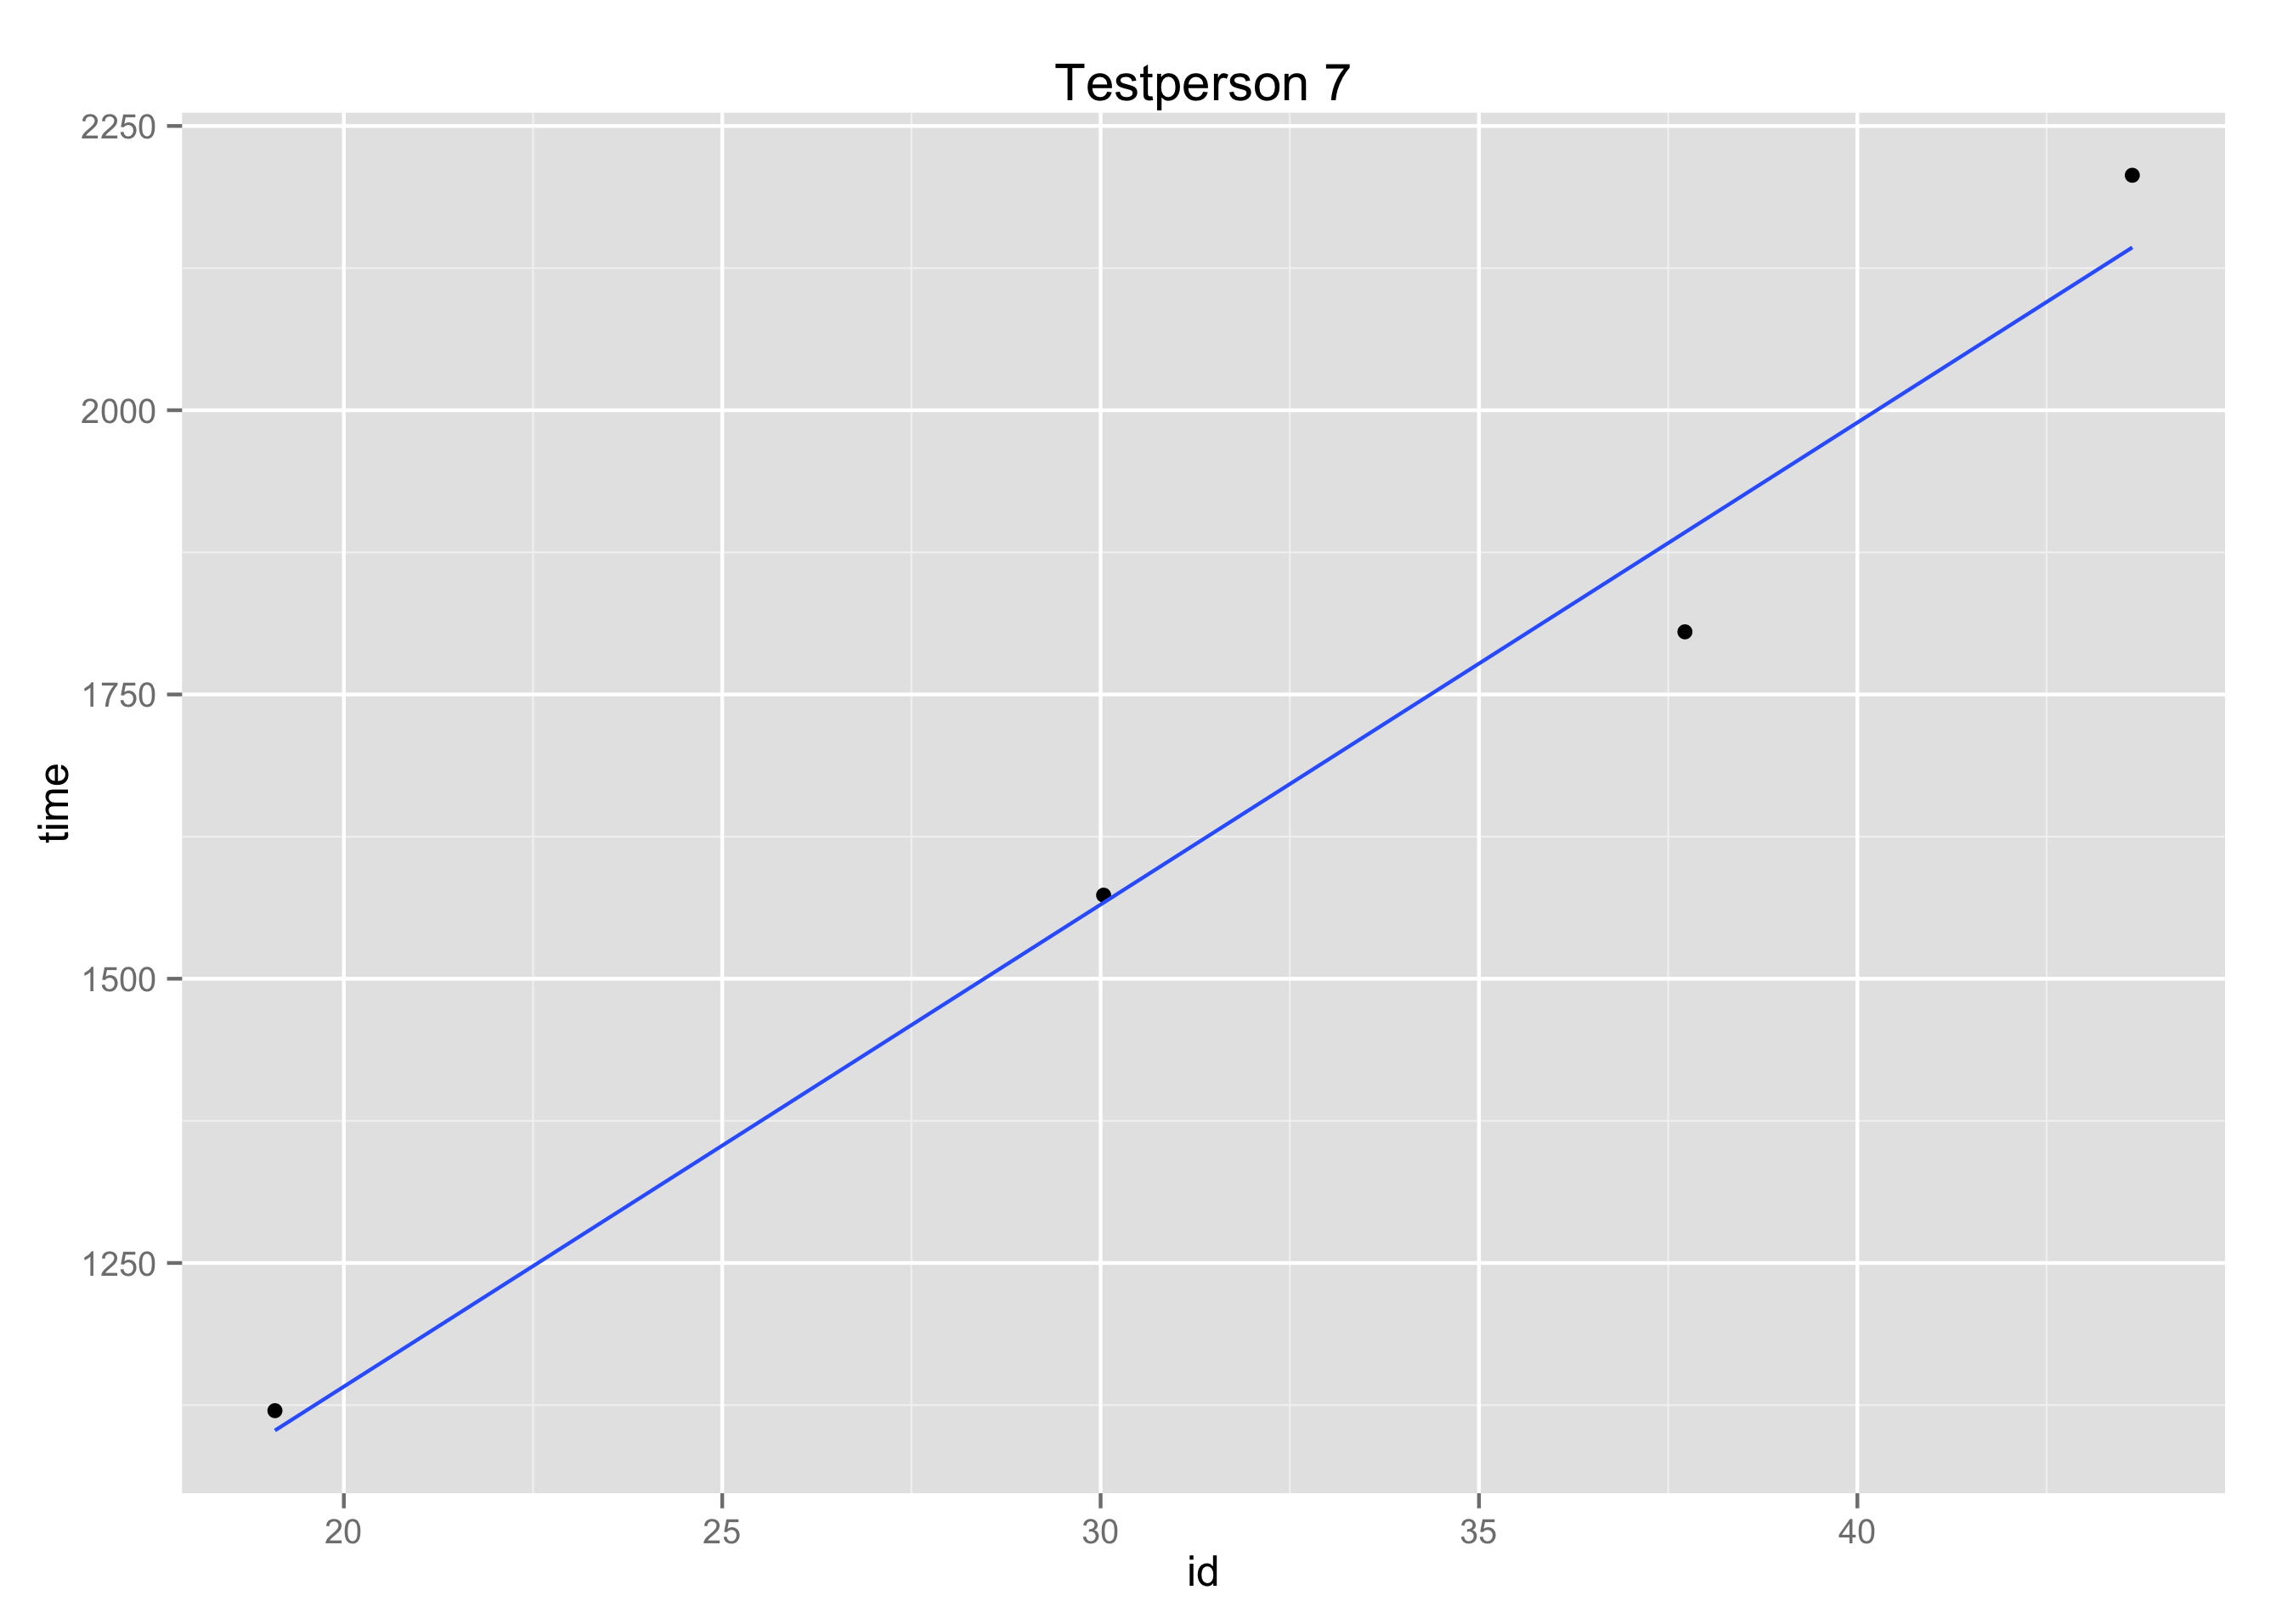
\includegraphics[width=\textwidth]{images/plots/plot_model_test_navigation_1}
		\captionof{figure}{Accot og Zhai's formulering tilpasset testperson 7's fire tunnelopgaver, med $ID$ på $x$-aksen og tiden $T$ på $y$-aksen}
		\label{fig:navigationtest1}
	\end{minipage}
	\begin{minipage}[b]{0.1\linewidth}
	~
	\end{minipage}
	\begin{minipage}[b]{0.45\linewidth}
		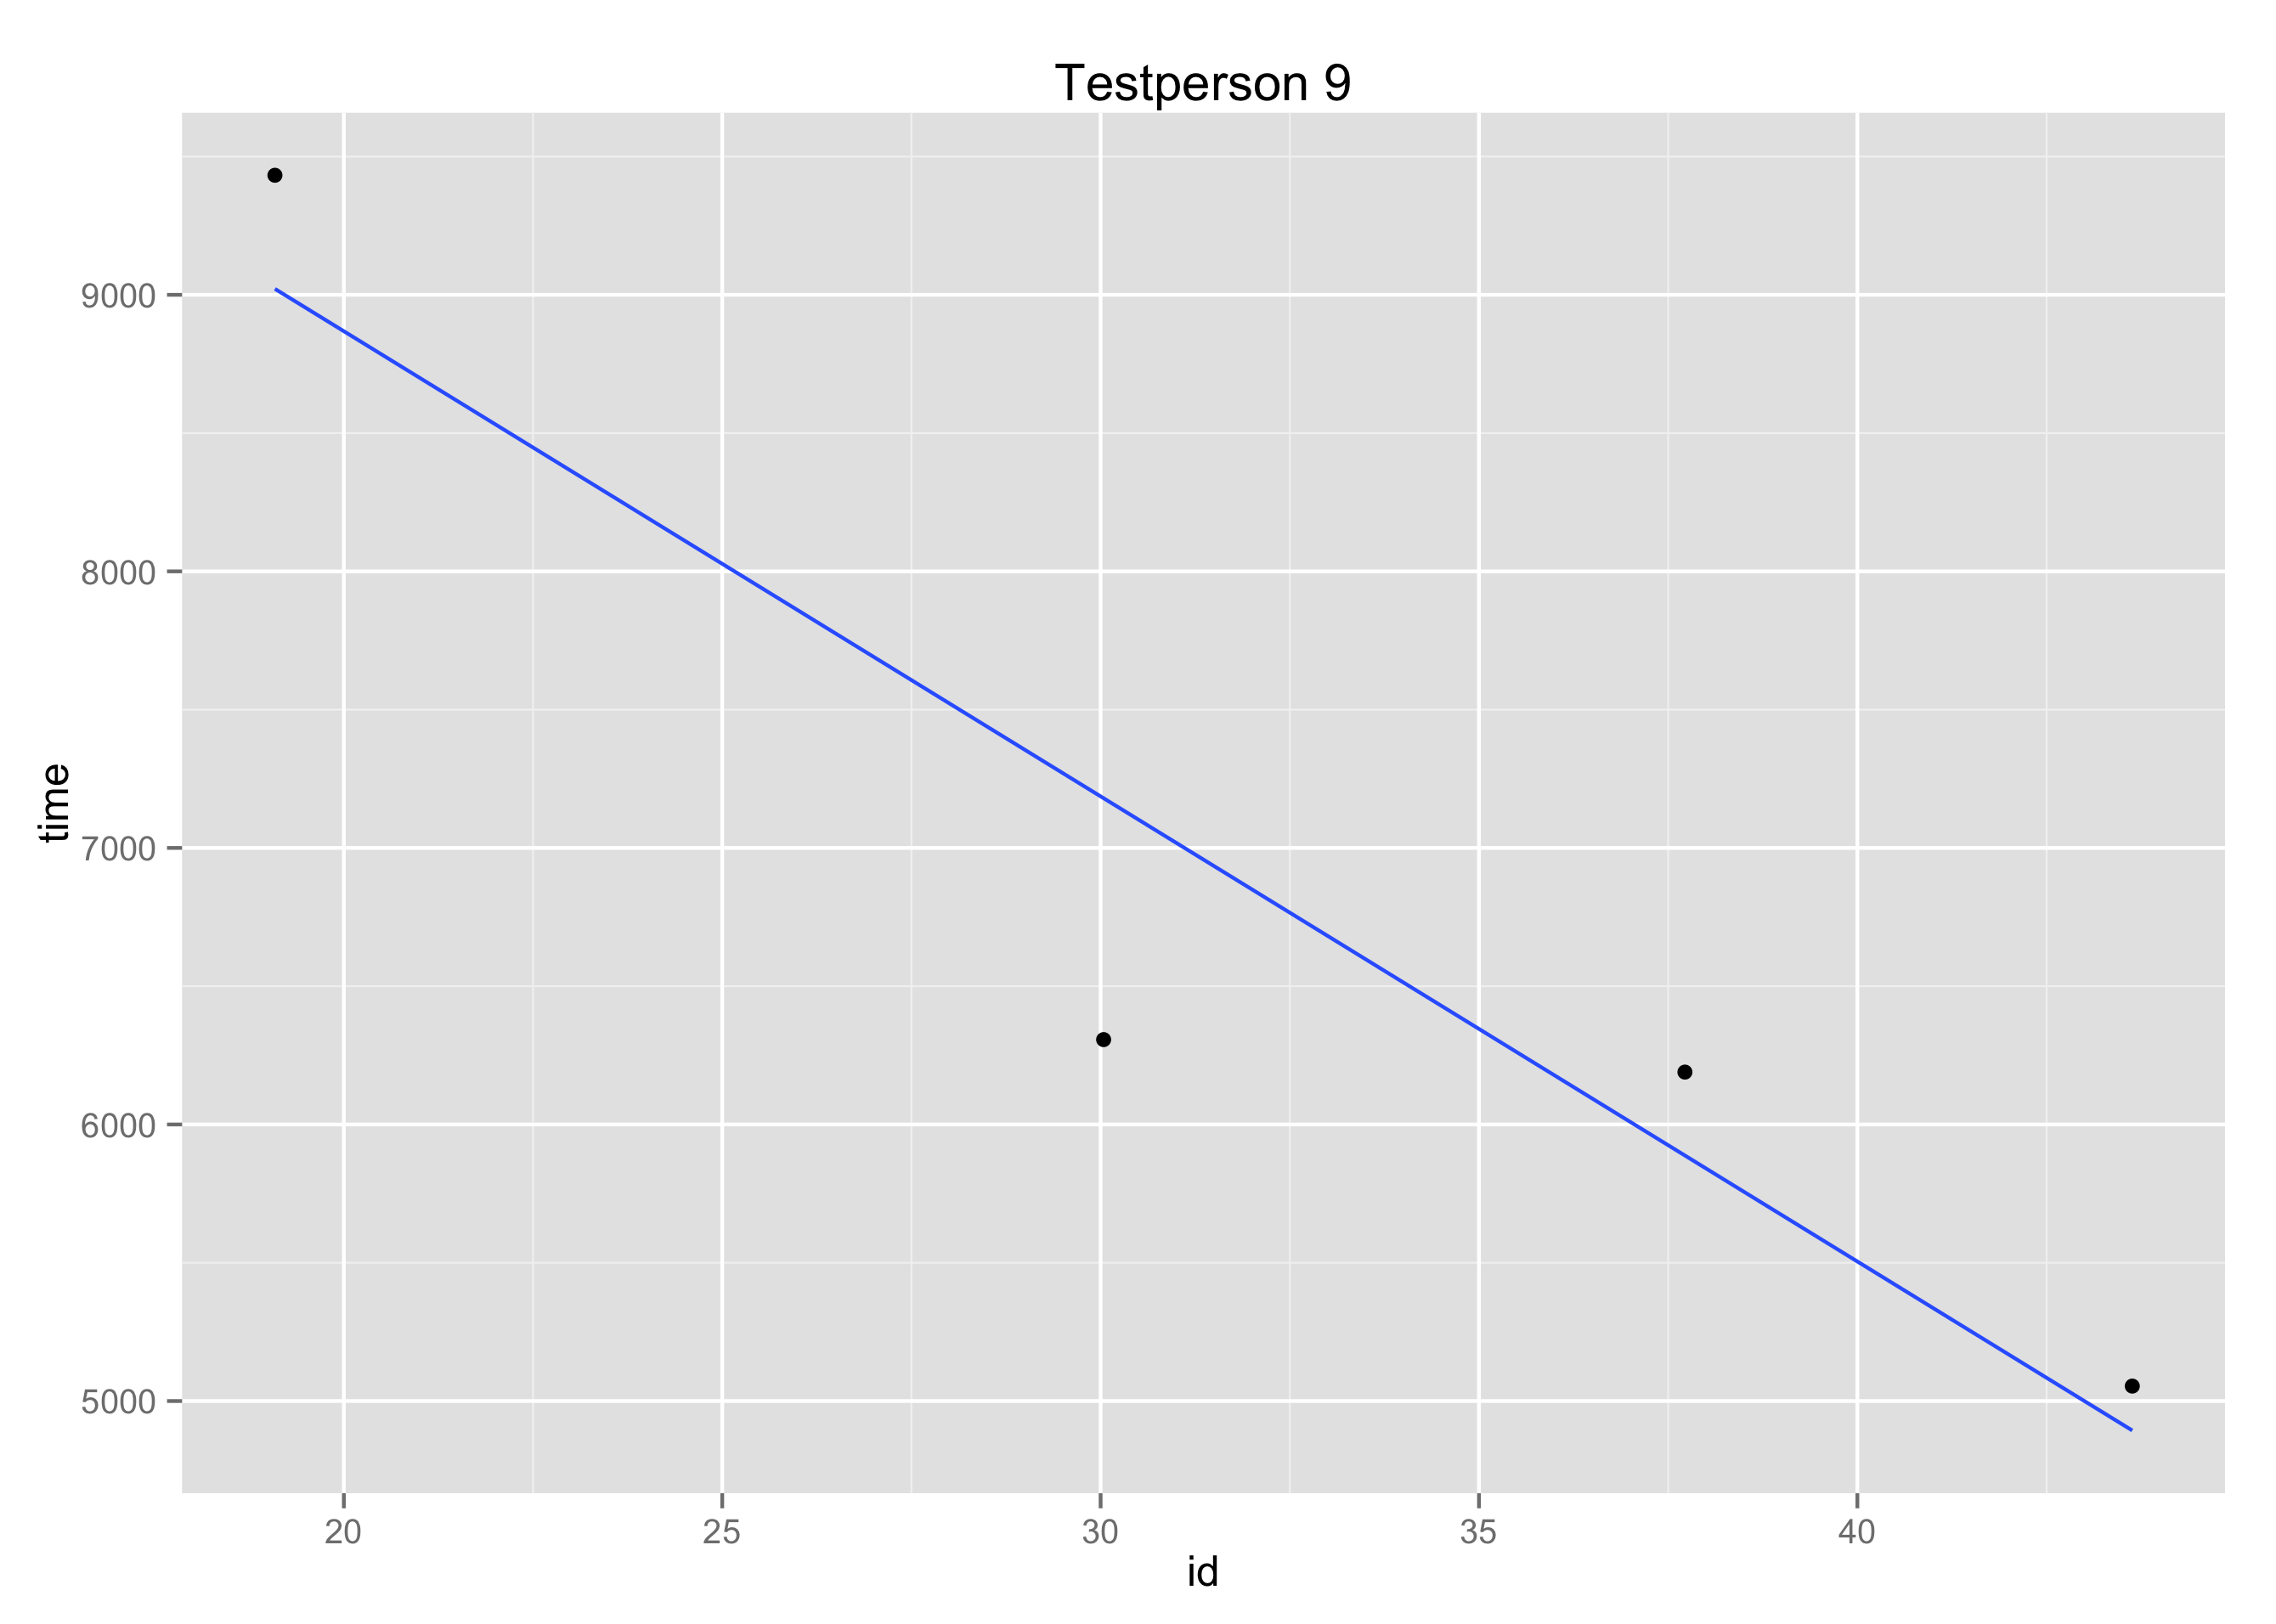
\includegraphics[width=\textwidth]{images/plots/plot_model_test_navigation_2}
		\captionof{figure}{Accot og Zhai's formulering tilpasset testperson 9's fire tunnelopgaver, med $ID$ på $x$-aksen og tiden $T$ på $y$-aksen}
		\label{fig:navigationtest2}
	\end{minipage}
\end{minipage}

\begin{minipage}{\linewidth}
	\begin{minipage}[t]{.45\linewidth}
		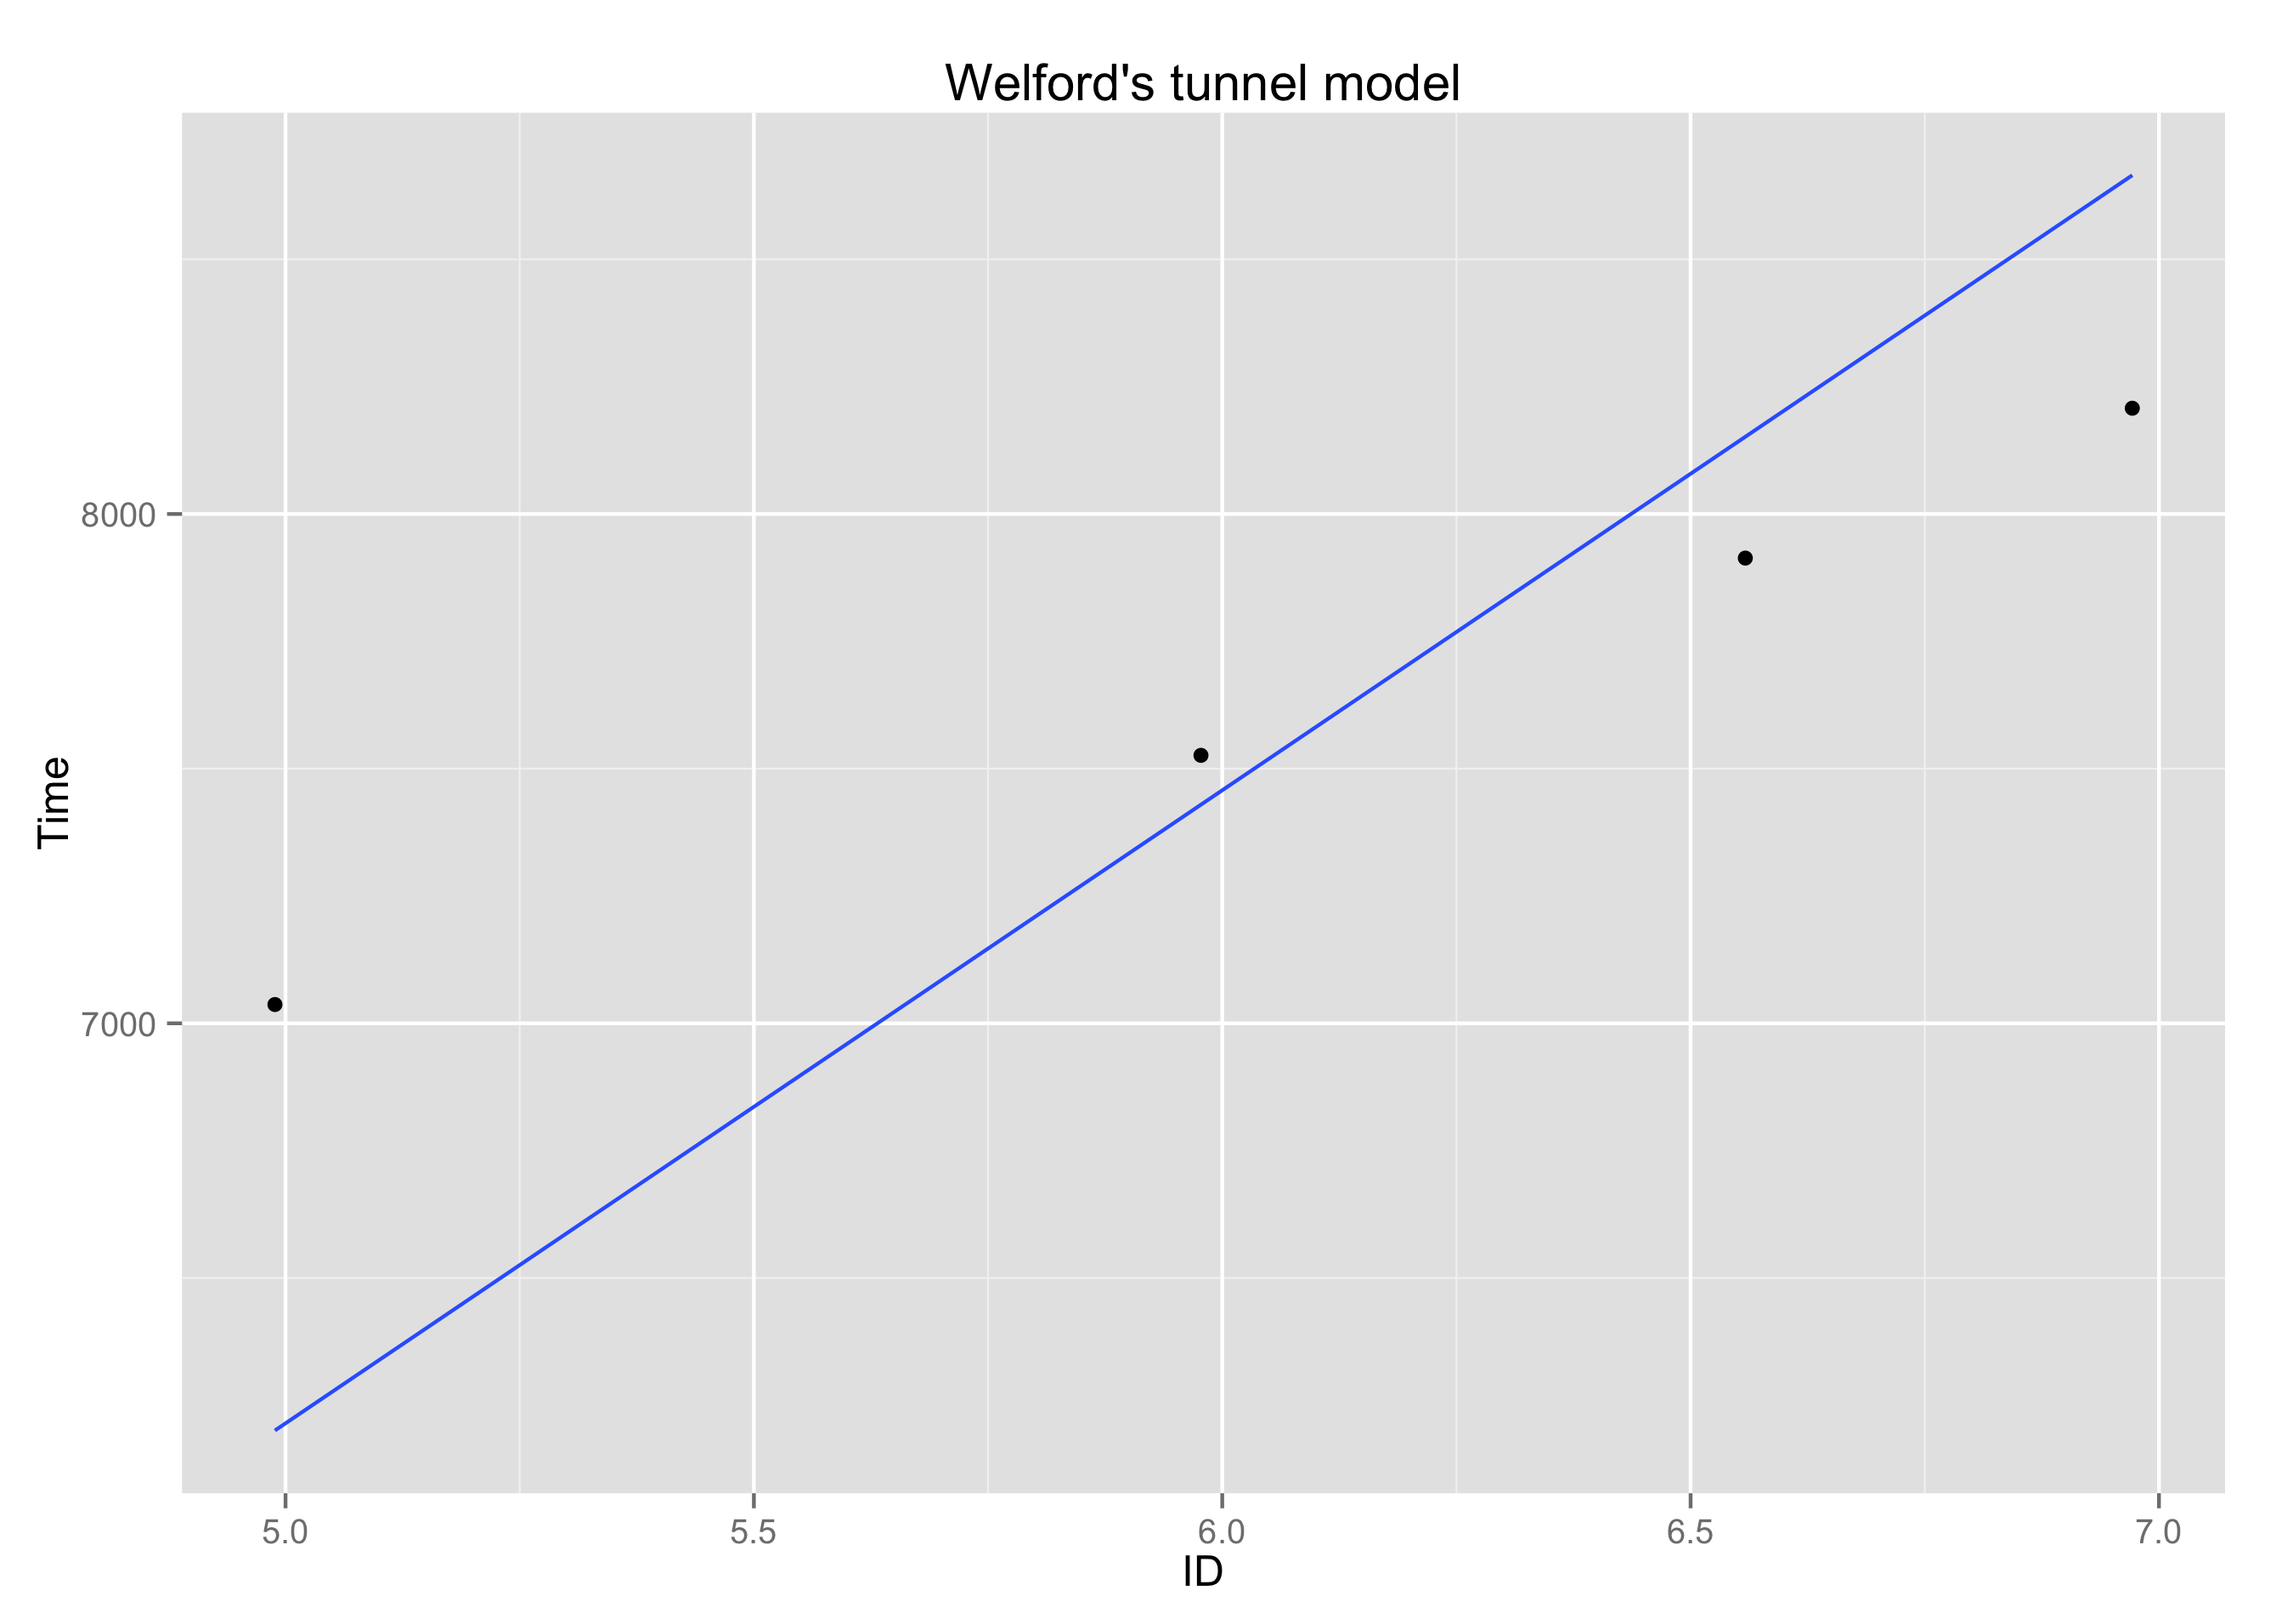
\includegraphics[width=\textwidth]{images/plots/plot_model_tunnel_welford}
		\captionof{figure}{Welford's lineære model tilpasset gennemsnitstiden pr. $ID$ for de 264 testdeltageres tunnelopgave. $ID$ på $x$-aksen og tiden $T$ på $y$-aksen}
		\label{fig:welford_tunnel_line}
	\end{minipage}
	\begin{minipage}[b]{0.1\linewidth}
	~
	\end{minipage}
	\begin{minipage}[t]{0.45\linewidth}
		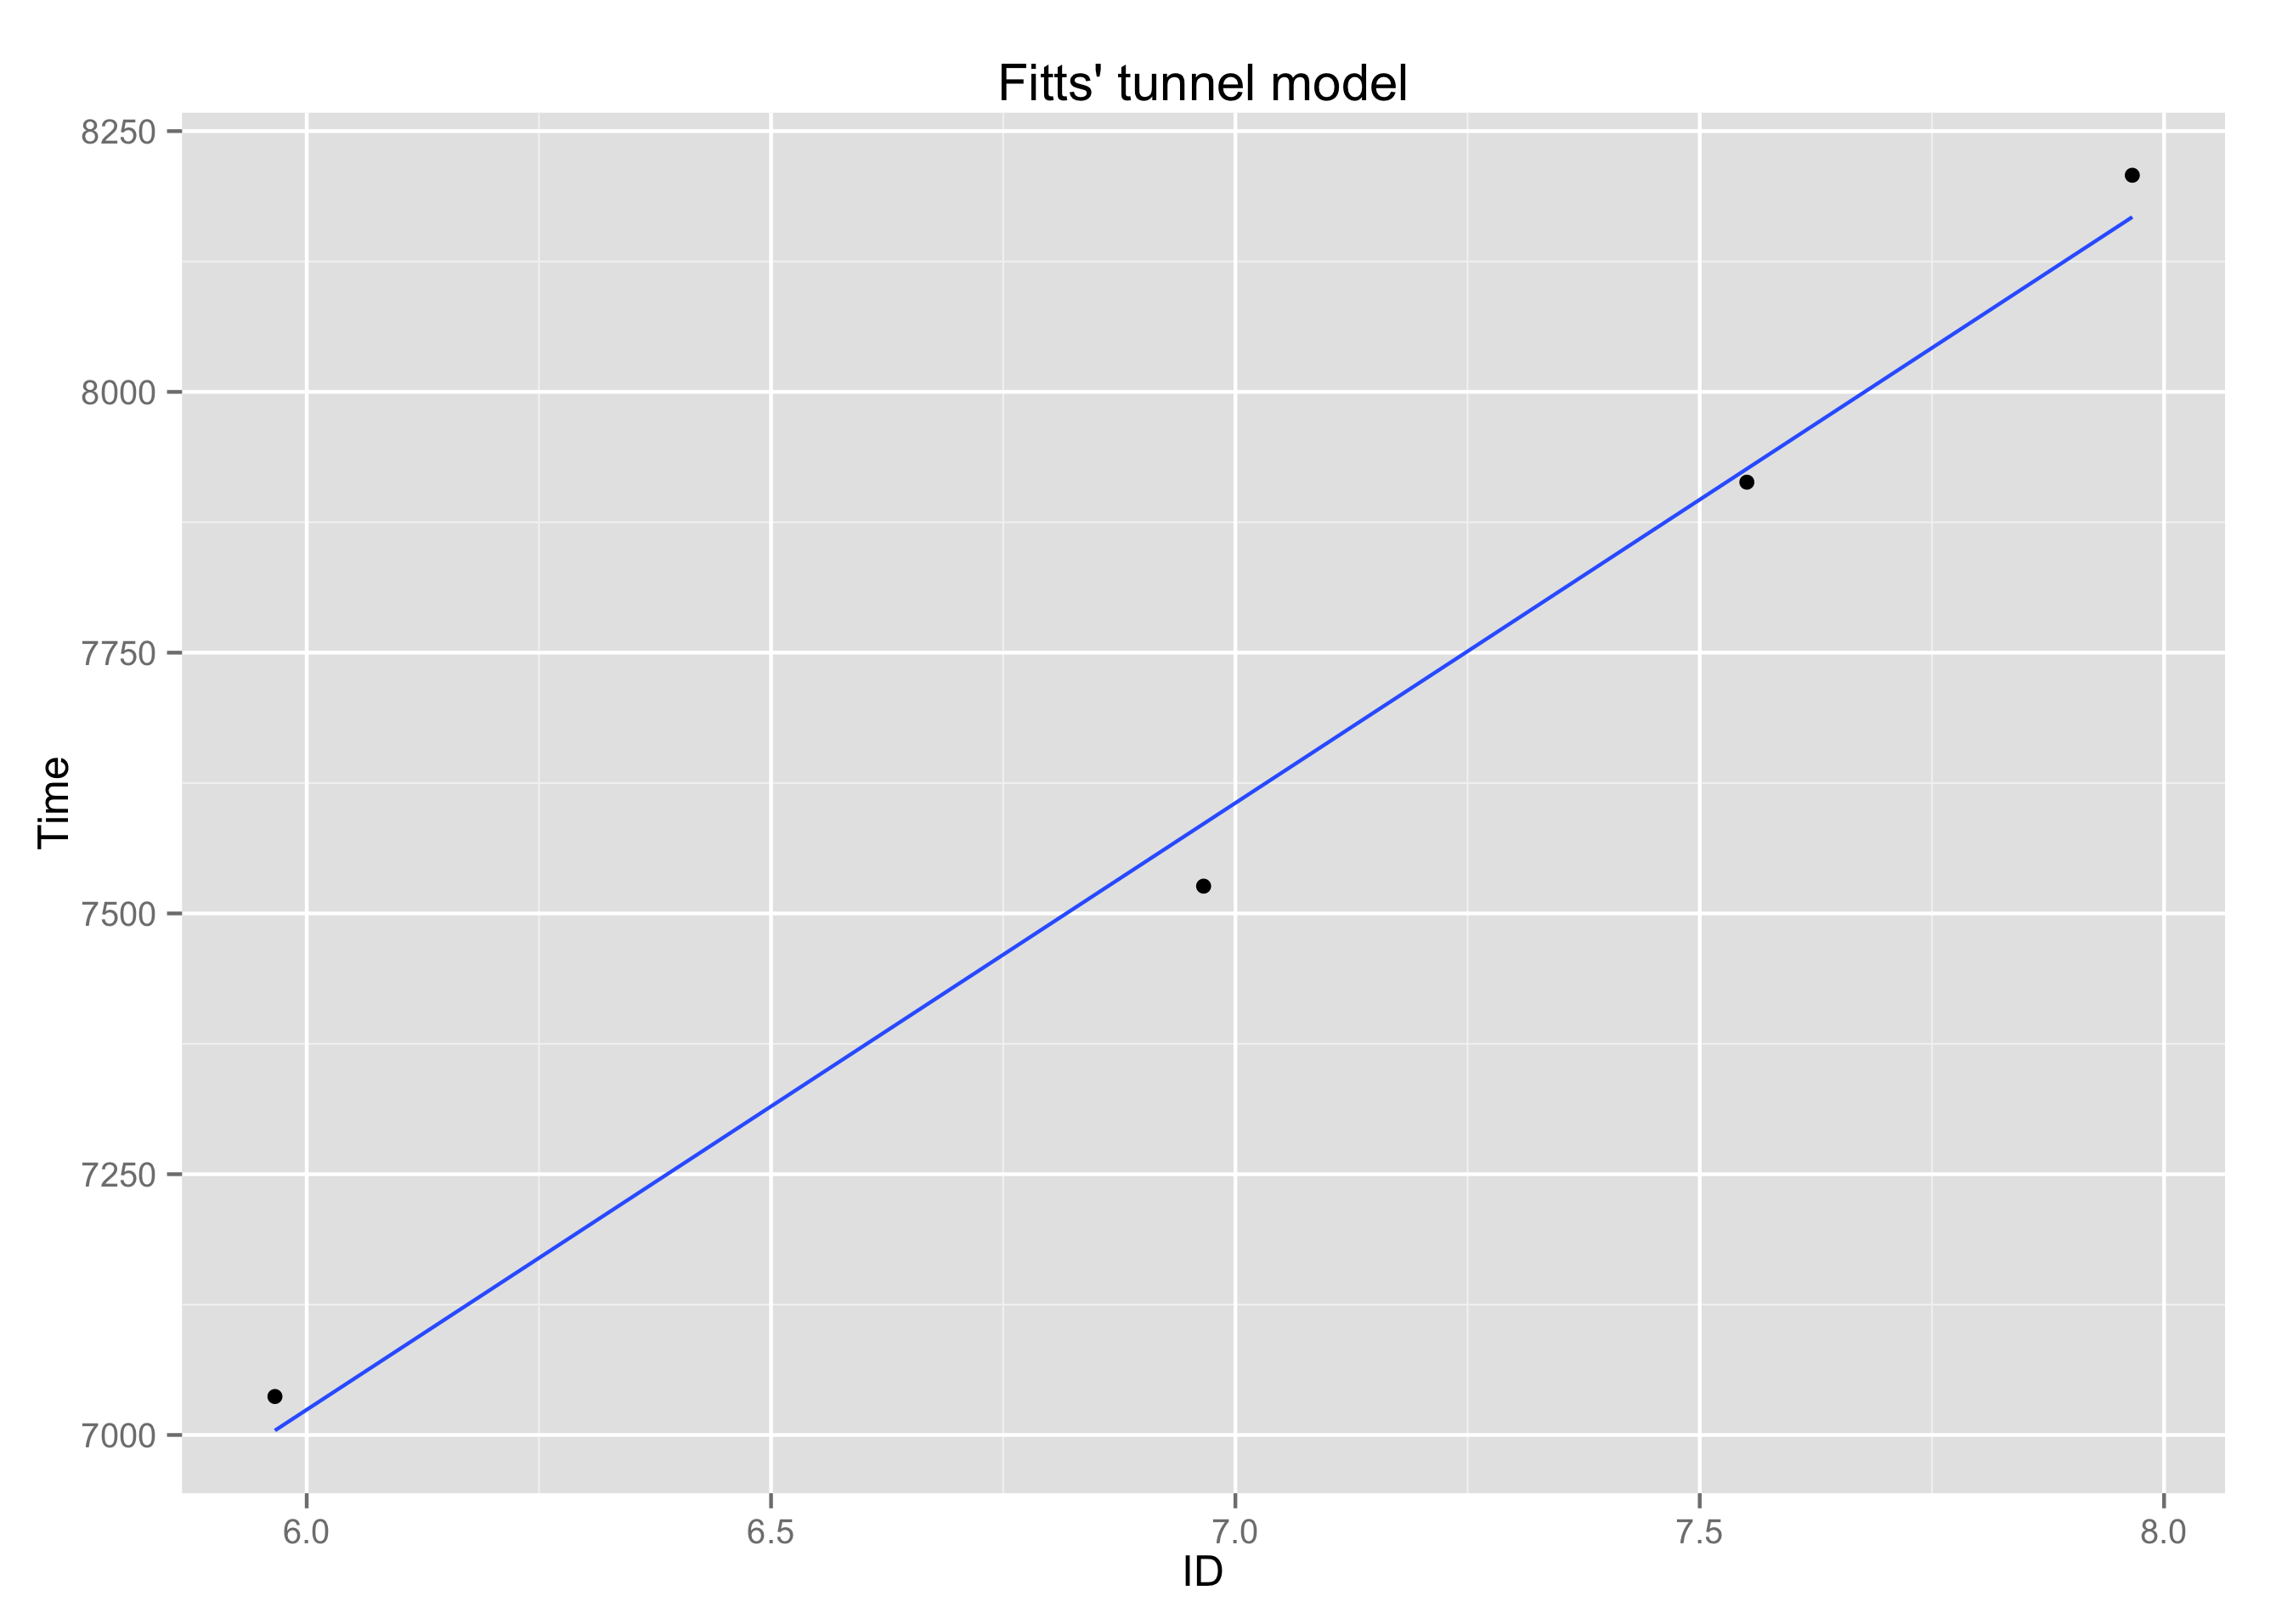
\includegraphics[width=\textwidth]{images/plots/plot_model_tunnel_fitt}
		\captionof{figure}{Fitts' affine model tilpasset gennemsnitstiden pr. $ID$ for de 264 testdeltageres tunnelopgave. $ID$ på $x$-aksen og tiden $T$ på $y$-aksen}
		\label{fig:fitt_tunnel_line}
	\end{minipage}
\end{minipage}
\begin{minipage}{\linewidth}
	\begin{minipage}[t]{.45\linewidth}
		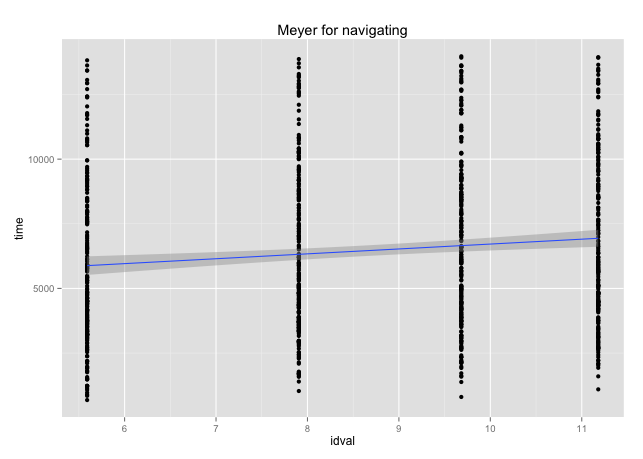
\includegraphics[width=\textwidth]{images/plots/plot_model_tunnel_meyer}
		\captionof{figure}{Meyer's affine model tilpasset gennemsnitstiden pr. $ID$ for de 264 testdeltageres tunnelopgave. $ID$ på $x$-aksen og tiden $T$ på $y$-aksen}
		\label{fig:meyer_tunnel_line}
	\end{minipage}
	\begin{minipage}[b]{0.1\linewidth}
	~
	\end{minipage}
	\begin{minipage}[t]{0.45\linewidth}
		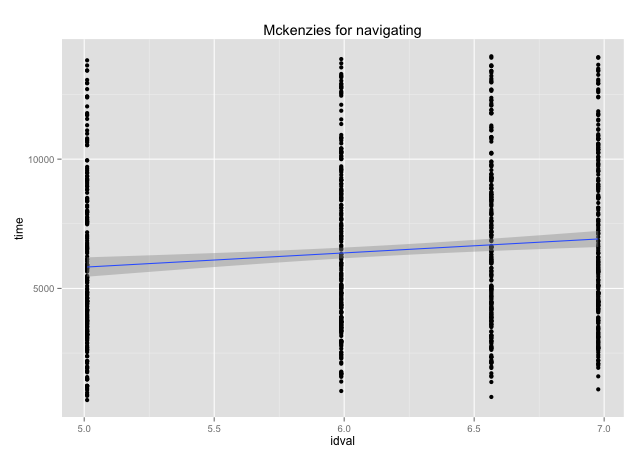
\includegraphics[width=\textwidth]{images/plots/plot_model_tunnel_mackenzie}
		\captionof{figure}{MacKenzie's affine model tilpasset gennemsnitstiden pr. $ID$ for de 264 testdeltageres tunnelopgave. $ID$ på $x$-aksen og tiden $T$ på $y$-aksen}
		\label{fig:mackenzie_tunnel_line}
	\end{minipage}
\end{minipage}
\begin{minipage}{\linewidth}
	\begin{minipage}[t]{\linewidth}
		\centering
		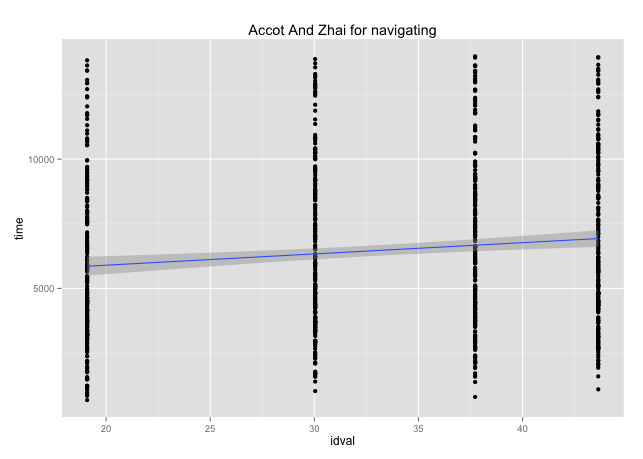
\includegraphics[width=0.5\textwidth]{images/plots/plot_model_tunnel_accot}
		\captionof{figure}{Accot \& Zhai's affine model tilpasset gennemsnitstiden pr. $ID$ for de 264 testdeltageres tunnelopgave. $ID$ på $x$-aksen og tiden $T$ på $y$-aksen}
		\label{fig:accot_tunnel_line}
	\end{minipage}
\end{minipage}

\newpage
\addcontentsline{toc}{subsection}{Analyse af spiralopgaver}
\subsection*{Analyse af spiralopgaver}
For at kunne tilpasse vores fire originale formuleringer af Fitts' lov, har vi defineret afstanden af $A$ som længden på spiralens bane i pixels. Disse afstande er bestemt på baggrund af antallet af vindinger i spiralen og resulterer i $A = [127,190,252,315]$. Bredden på målet, $W$, har vi valgt som længden på den inderste vandrette linje i spiralen, slutstregen, som altid er 25 pixels bred. Ved disse værdier kan vi tilpasse formuleringernes tilhørende $ID$ og tiden, $T$, per opgave til en affin model, med $lm$, for alle 264 testdeltageres spiralopgavedatapunkter. De fire matematiske modelfremstillinger med respektive konstanter er vist nedenfor.
\begin{align*}
\text{Fitts': } &T = -24882.5+ 8217.7 \cdot \log_2\left(\frac{2A}{W}\right)\\
\text{Welford's: } &T =  2808.54\cdot \log_2\left(\frac{A+\frac{1}{2}W}{W}\right)\\
\text{MacKenzie's: } &T = -21606.0 + 9310.7\cdot \log_2\left(\frac{A+W}{W}\right)\\
\text{Meyer's: } &T = -16269.1 + 8452.2 \cdot \sqrt{\frac{A}{W}}
\end{align*}

Accot og Zhai argumenterer i \cite{accot1997} for, at $ID$ for en navigationsopgave med en spiral, kan findes ved at opdele den i delelementer baseret på vinklen $\theta$. Ved hvert delelement kan bredden, $w$, findes og alle delelementerne summeres ved et integral over vinklerne på baggrund af antallet vindinger, $n$. Dette integral, vist nedenfor, giver i følge Accot og Zhai et $ID_s$, som er specifikt for denne type navigationsopgaver. 
\begin{align*}
ID_s = \int_{2\pi}^{2\pi(n+1)}\frac{\sqrt{\left(\theta+w\right)^6+9\left(\theta+w\right)^4}}{\left(\theta+2\pi+2\right)^3-\left(\theta+w\right)^3}d\theta
\end{align*}

For vores spiralopgaver gjorde vi brug af $n=[1,2,3,4], w=[3.1,3.1,3.1,3.05]$. For hver testdeltager i vores kontrollerede eksperiment har vi tilpasset deres tid, $T$, og de fire udregnede $ID_s$ med lineær regression. Figur \ref{fig:spiralingtest1} og \ref{fig:spiralingtest2} viser de affine modellers tilpasning til de fire datapunkter for henholdvis testperson 2 og 10. Det kan bemærkes, hvordan kurven er monotont voksende, hvilket stemmer overens med forventningen om, at det tager længere tid at gennemføre en opgave, hvis $ID$ bliver højere. I modsætning til tunnelopgaven var der ingen af testpersonerne i det kontrollerede forsøg, som blev hurtigere ved højere $ID$.\\\\
\begin{minipage}{\linewidth}
	\begin{minipage}[b]{.45\linewidth}
		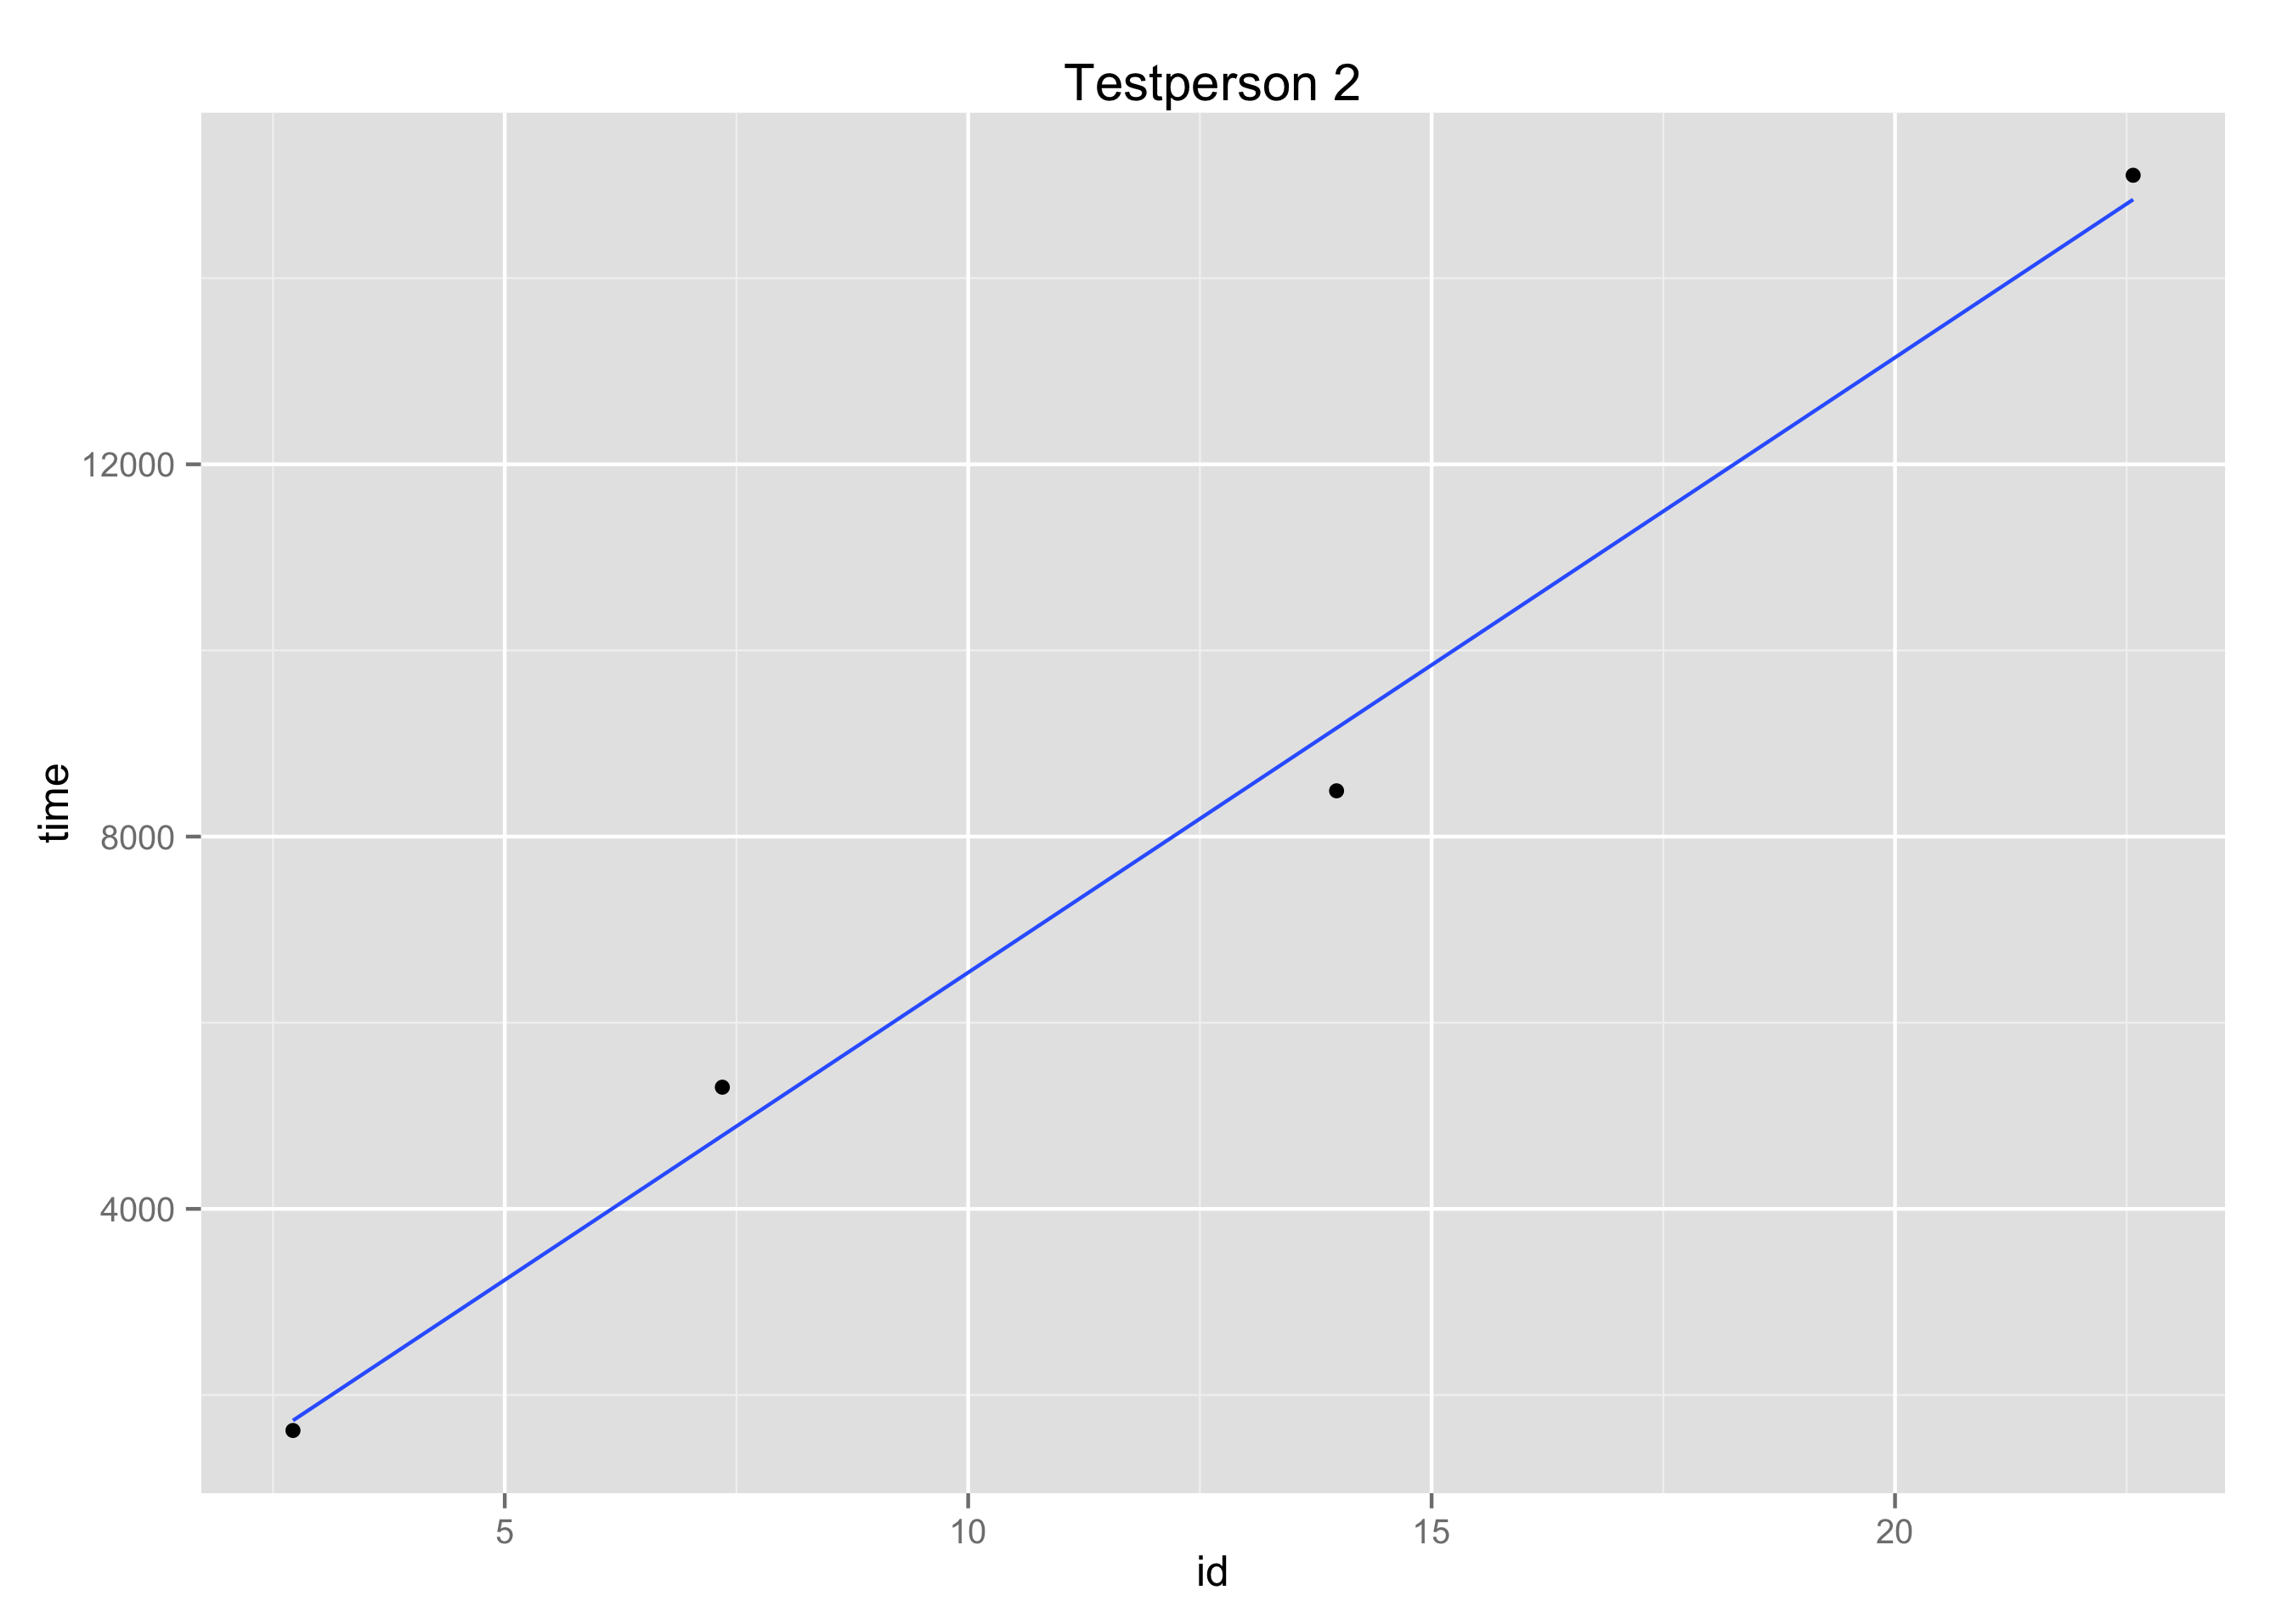
\includegraphics[width=\textwidth]{images/plots/plot_model_test_spiraling_1}
		\captionof{figure}{Accot og Zhai's formulering tilpasset testperson 2, med $ID_s$ på $x$-aksen og tiden $T$ på $y$-aksen}
		\label{fig:spiralingtest1}
	\end{minipage}
	\begin{minipage}[b]{0.1\linewidth}
	~
	\end{minipage}
	\begin{minipage}[b]{0.45\linewidth}
		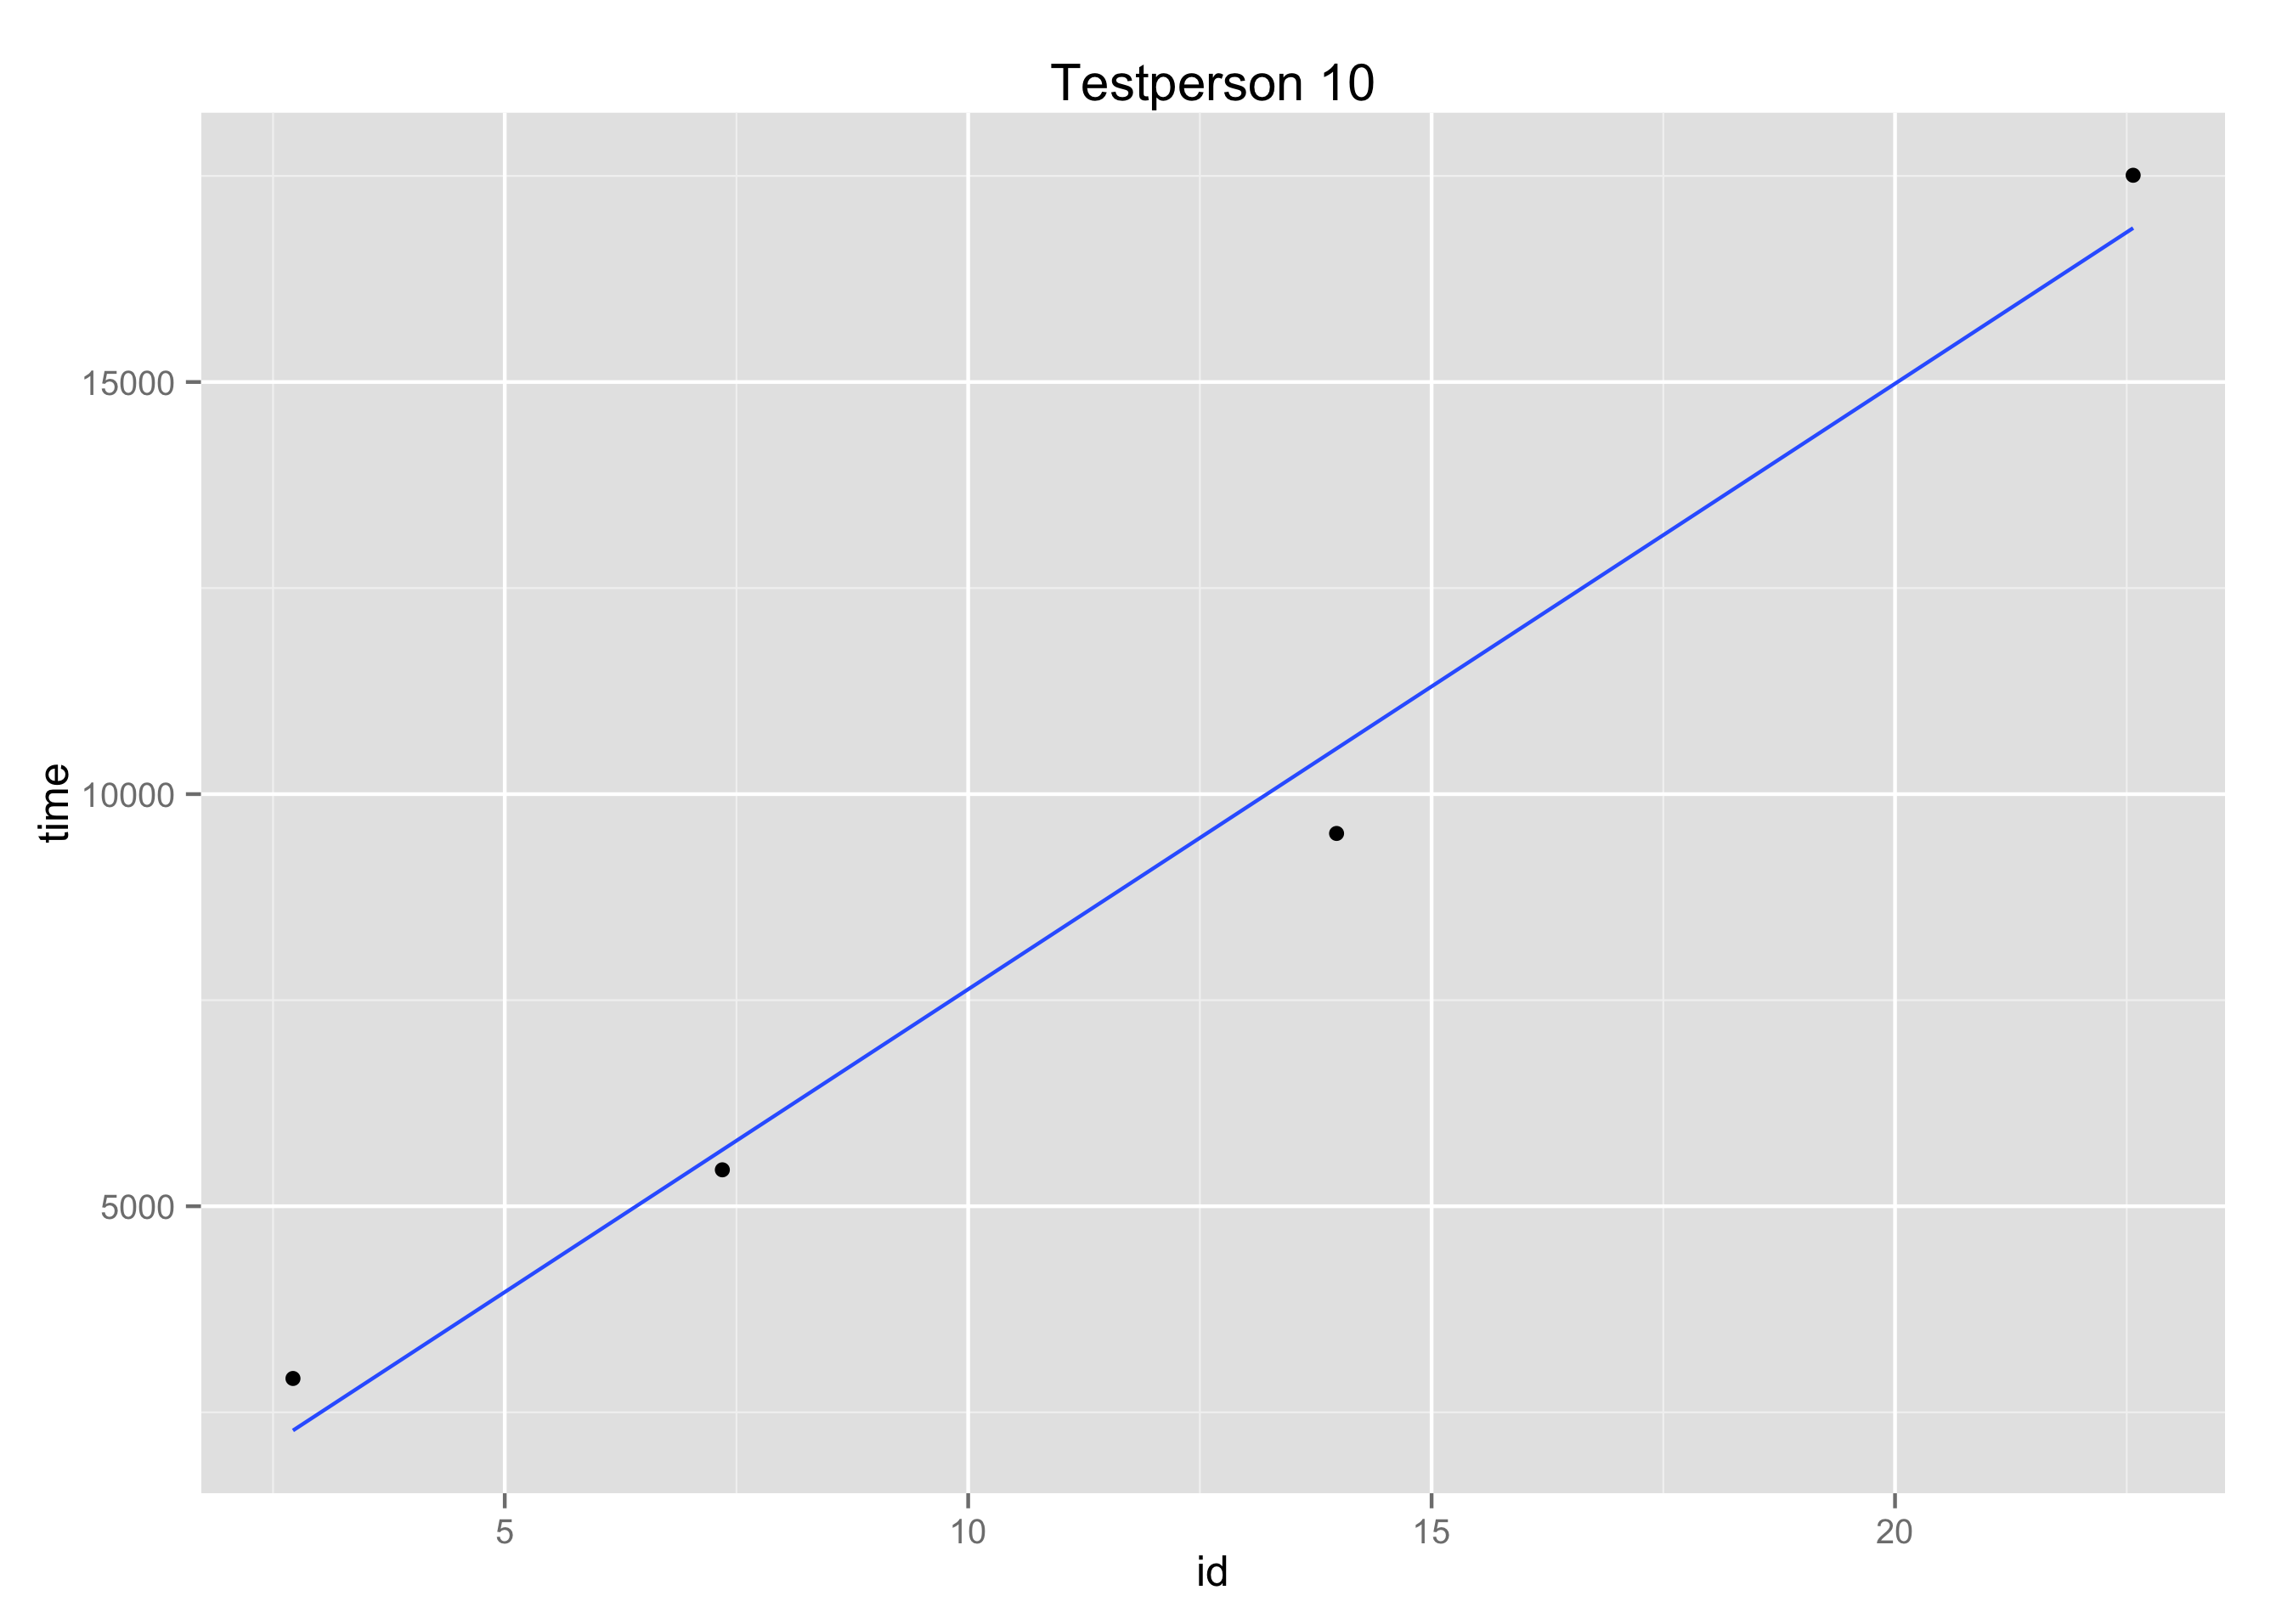
\includegraphics[width=\textwidth]{images/plots/plot_model_test_spiraling_2}
		\captionof{figure}{Accot og Zhai's formulering tilpasset testperson 10, med $ID_s$ på $x$-aksen og tiden $T$ på $y$-aksen}
		\label{fig:spiralingtest2}
	\end{minipage}
\end{minipage}

\newpage
Ved at tilpasse Accot og Zhai's $ID_s$ til vores 264 testdeltageres spiralopgavedata fandt vi frem til den matematiske model i (\ref{eq:accotspiral}). Det kan bemærkes, at de to konstante led for denne model er markant anderledes end de tilsvarende for de fire andre formuleringer.  AIC-analyserne i tabel \ref{tab:table_analysis_aic_spiral_all} og \ref{tab:table_analysis_aic_spiral_mean} viser, hvordan Accot og Zhai's formulering klarer sig væsentligt bedre end de fire andres. Det gælder både for alle datapunkterne og for gennemsnitsværdierne. Dette er også, hvad vi forventede, da de fire originale formuleringer ikke er beregnet til denne type navigationsopgaver, imens Accot og Zhai's er tiltænkt til denne type.
\begin{align}
\text{Accot \& Zhai: } T = 2097.09+553.25 \cdot \int_{2\pi}^{2\pi(n+1)}\frac{\sqrt{\left(\theta+w\right)^6+9\left(\theta+w\right)4}}{\left(\theta+2\pi+2\right)^3-\left(\theta+w\right)^3}d\theta
\label{eq:accotspiral}
\end{align}

Ligesom for vores tunnelopgaver har vi valgt at visualisere de fem modellers tilpasning til spiralopgaverne, ved at bruge gennemsnitstiden for hver $ID$ som datapunkter. De fem affine kurver og tilhørende fire datapunkter kan ses i figur \ref{fig:welford_spiral_line}-\ref{fig:accot_spiral_line}.\\\\
\begin{minipage}[t]{\linewidth}
	\begin{minipage}[t]{0.45\linewidth}
		\begin{tabular}{lll}
			Model & AIC-værdi & Forskel\\\hline
			Accot \& Zhai & 20225.67 & 0\\
			Meyer & 20240.39 & 14.72 \\
			MacKenzie & 20256.62 & 30.95\\
			Fitts & 20262.07 & 36.4\\
			Welford & 20613.96 & 388.29
		\end{tabular}
		\captionof{table}{AIC-værdier for de 264 testdeltageres spiralopgaver. Deres indbyrdes forskel er beregnet med udgangspunkt i Accot \& Zhai's formulering som nulpunkt}
		\label{tab:table_analysis_aic_spiral_all}
	\end{minipage}
	\begin{minipage}[t]{0.1\linewidth}
	~
	\end{minipage}
	\begin{minipage}[t]{0.45\linewidth}
		\begin{tabular}{lll}
			Model & AIC-værdi & Forskel\\\hline
			Accot \& Zhai & 61.91 & 0\\
			Meyer & 68.12 & 6.21 \\
			MacKenzie & 70.66 & 8.75\\
			Fitts & 71.25 & 9.34\\
			Welford & 79.11 & 17.2
		\end{tabular}
		\captionof{table}{AIC-værdier for gennemsnittet af tiderne for de 264 testdeltageres spiralopgaver ved hvert $ID$. Deres indbyrdes forskel er beregnet med udgangspunkt i Accot \& Zhai's formulering som nulpunkt}
		\label{tab:table_analysis_aic_spiral_mean}
	\end{minipage}
\end{minipage}\\\\
\begin{minipage}{\linewidth}
	\begin{minipage}[t]{.45\linewidth}
		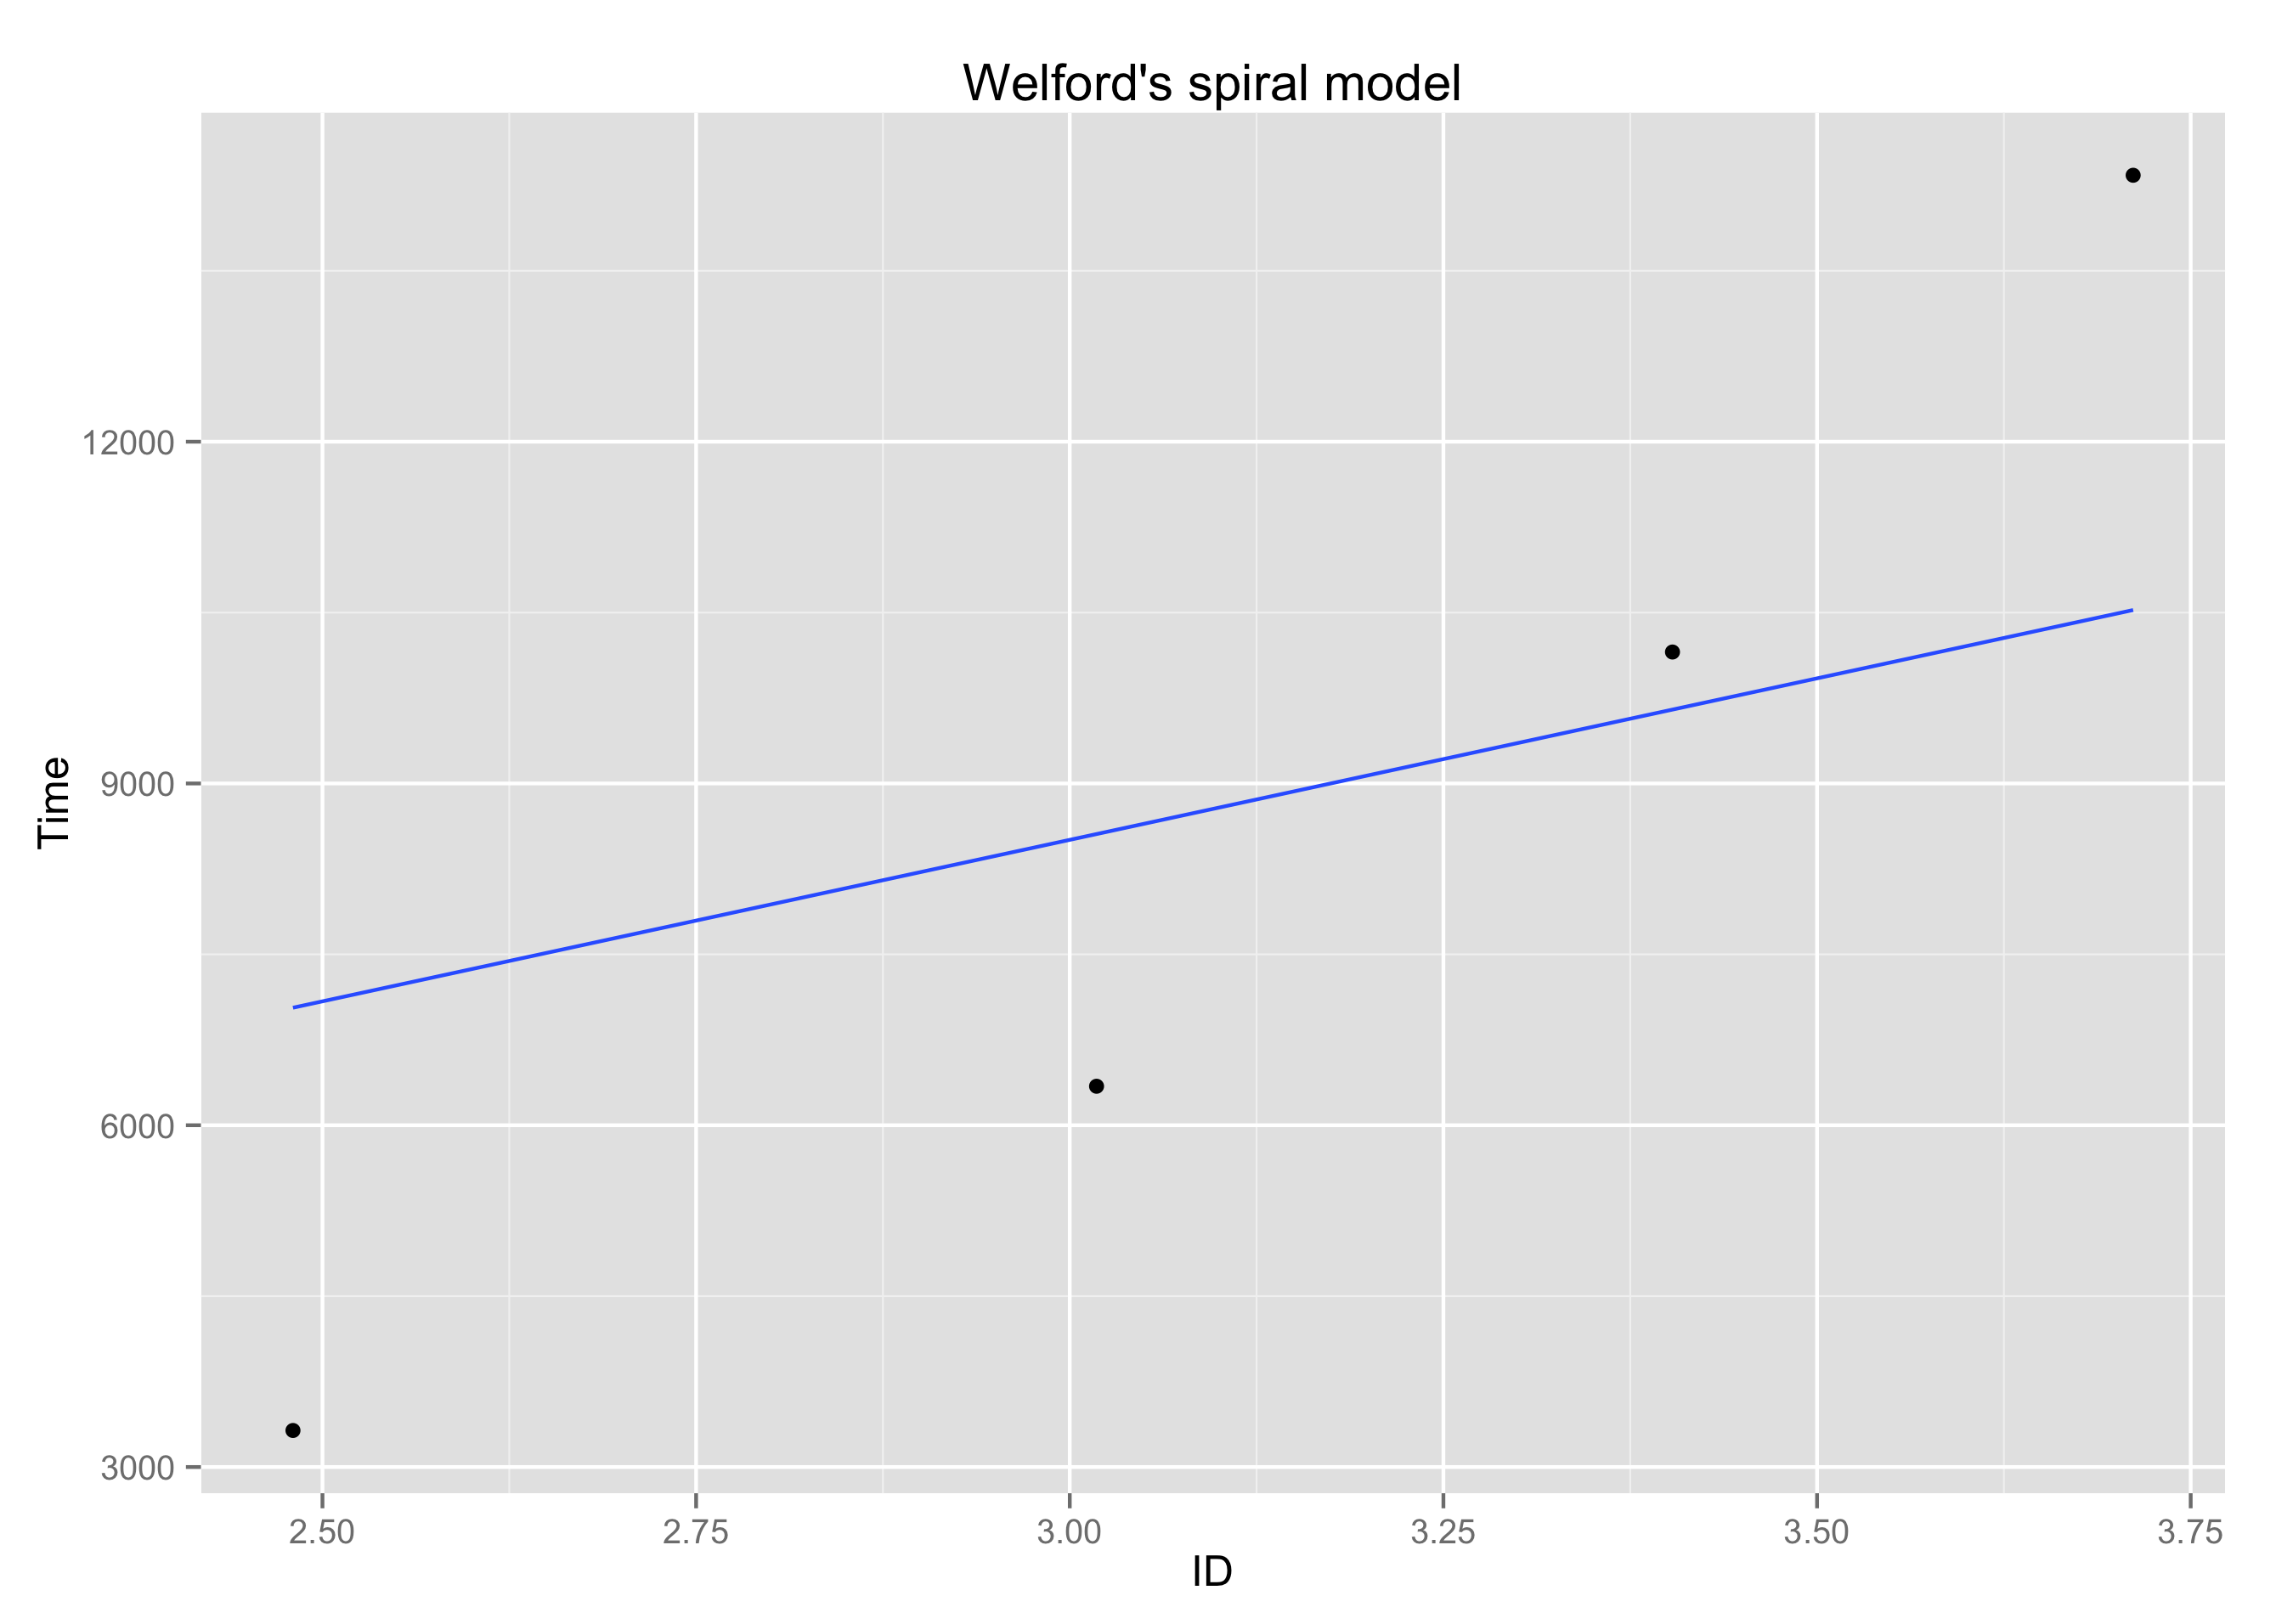
\includegraphics[width=\textwidth]{images/plots/plot_model_spiral_welford}
		\captionof{figure}{Welford's lineære model til gennemsnitstiden per $ID$, med $ID$ på $x$-aksen og tiden $T$ på $y$-aksen}
		\label{fig:welford_spiral_line}
	\end{minipage}
	\begin{minipage}[b]{0.1\linewidth}
	~
	\end{minipage}
	\begin{minipage}[t]{0.45\linewidth}
		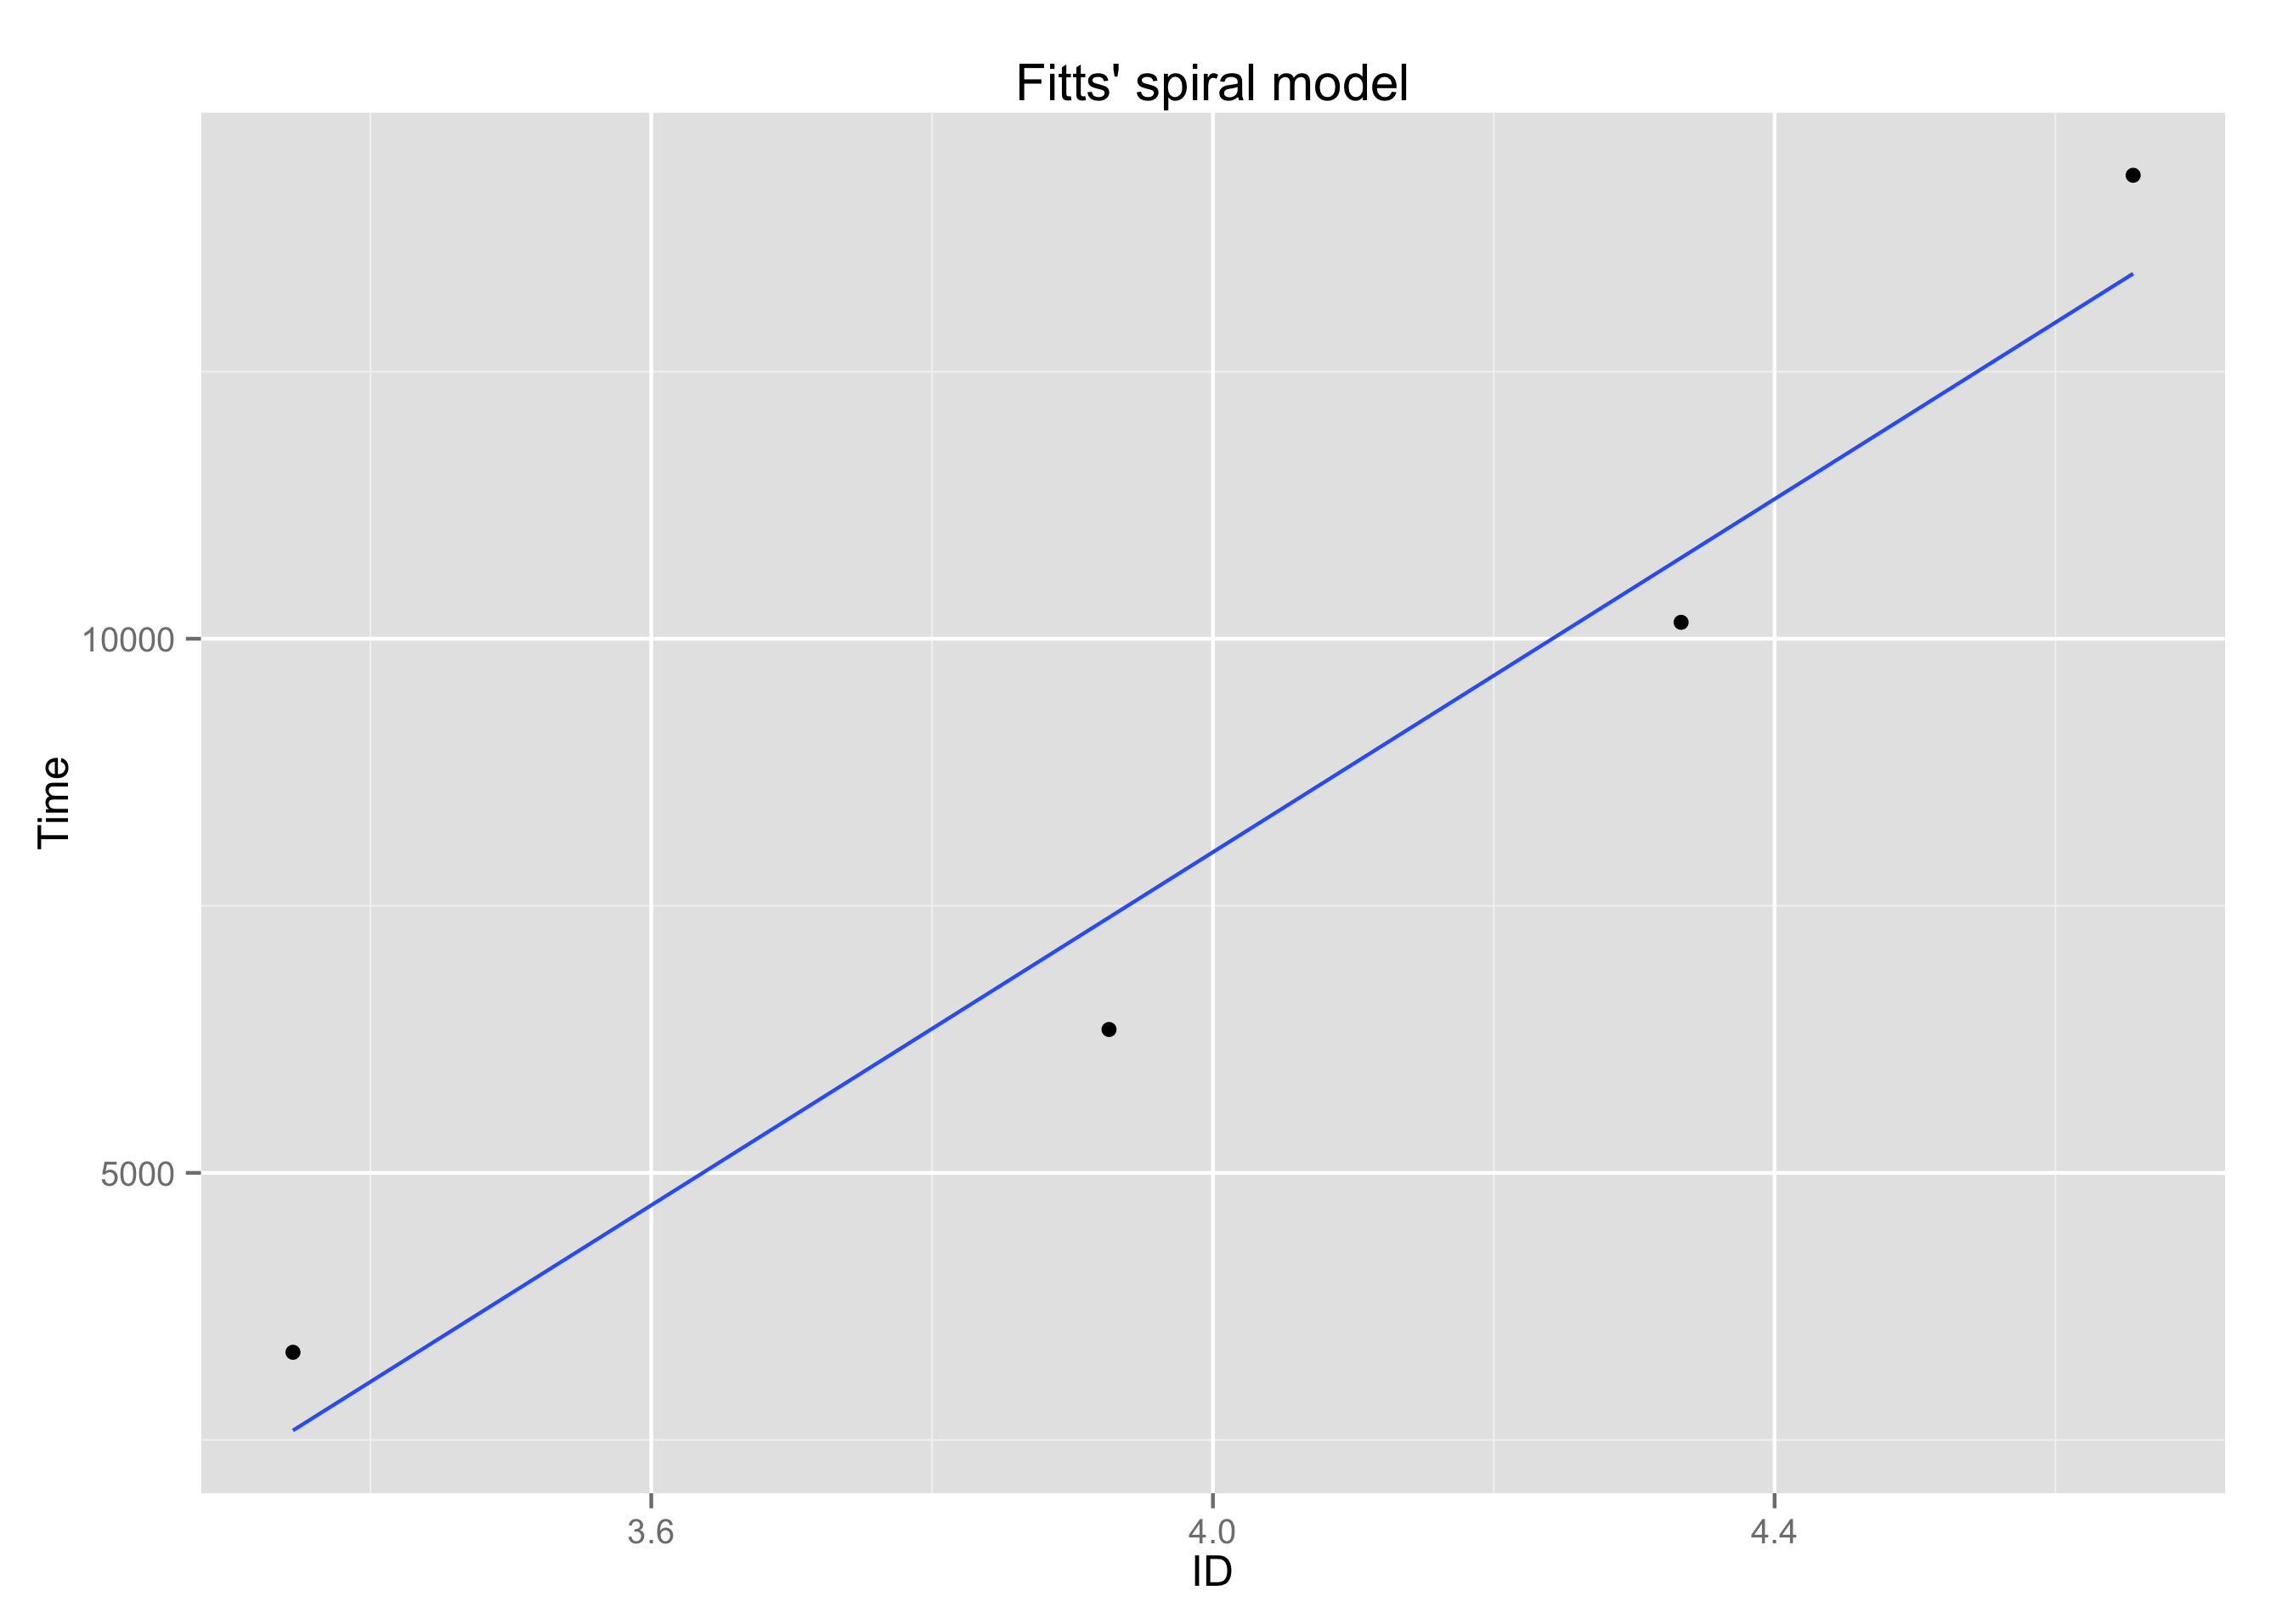
\includegraphics[width=\textwidth]{images/plots/plot_model_spiral_fitt}
		\captionof{figure}{Fitts' affine model til gennemsnitstiden per $ID$, med $ID$ på $x$-aksen og tiden $T$ på $y$-aksen}
		\label{fig:fitt_spiral_line}
	\end{minipage}
\end{minipage}
\begin{minipage}{\linewidth}
	\begin{minipage}[t]{.45\linewidth}
		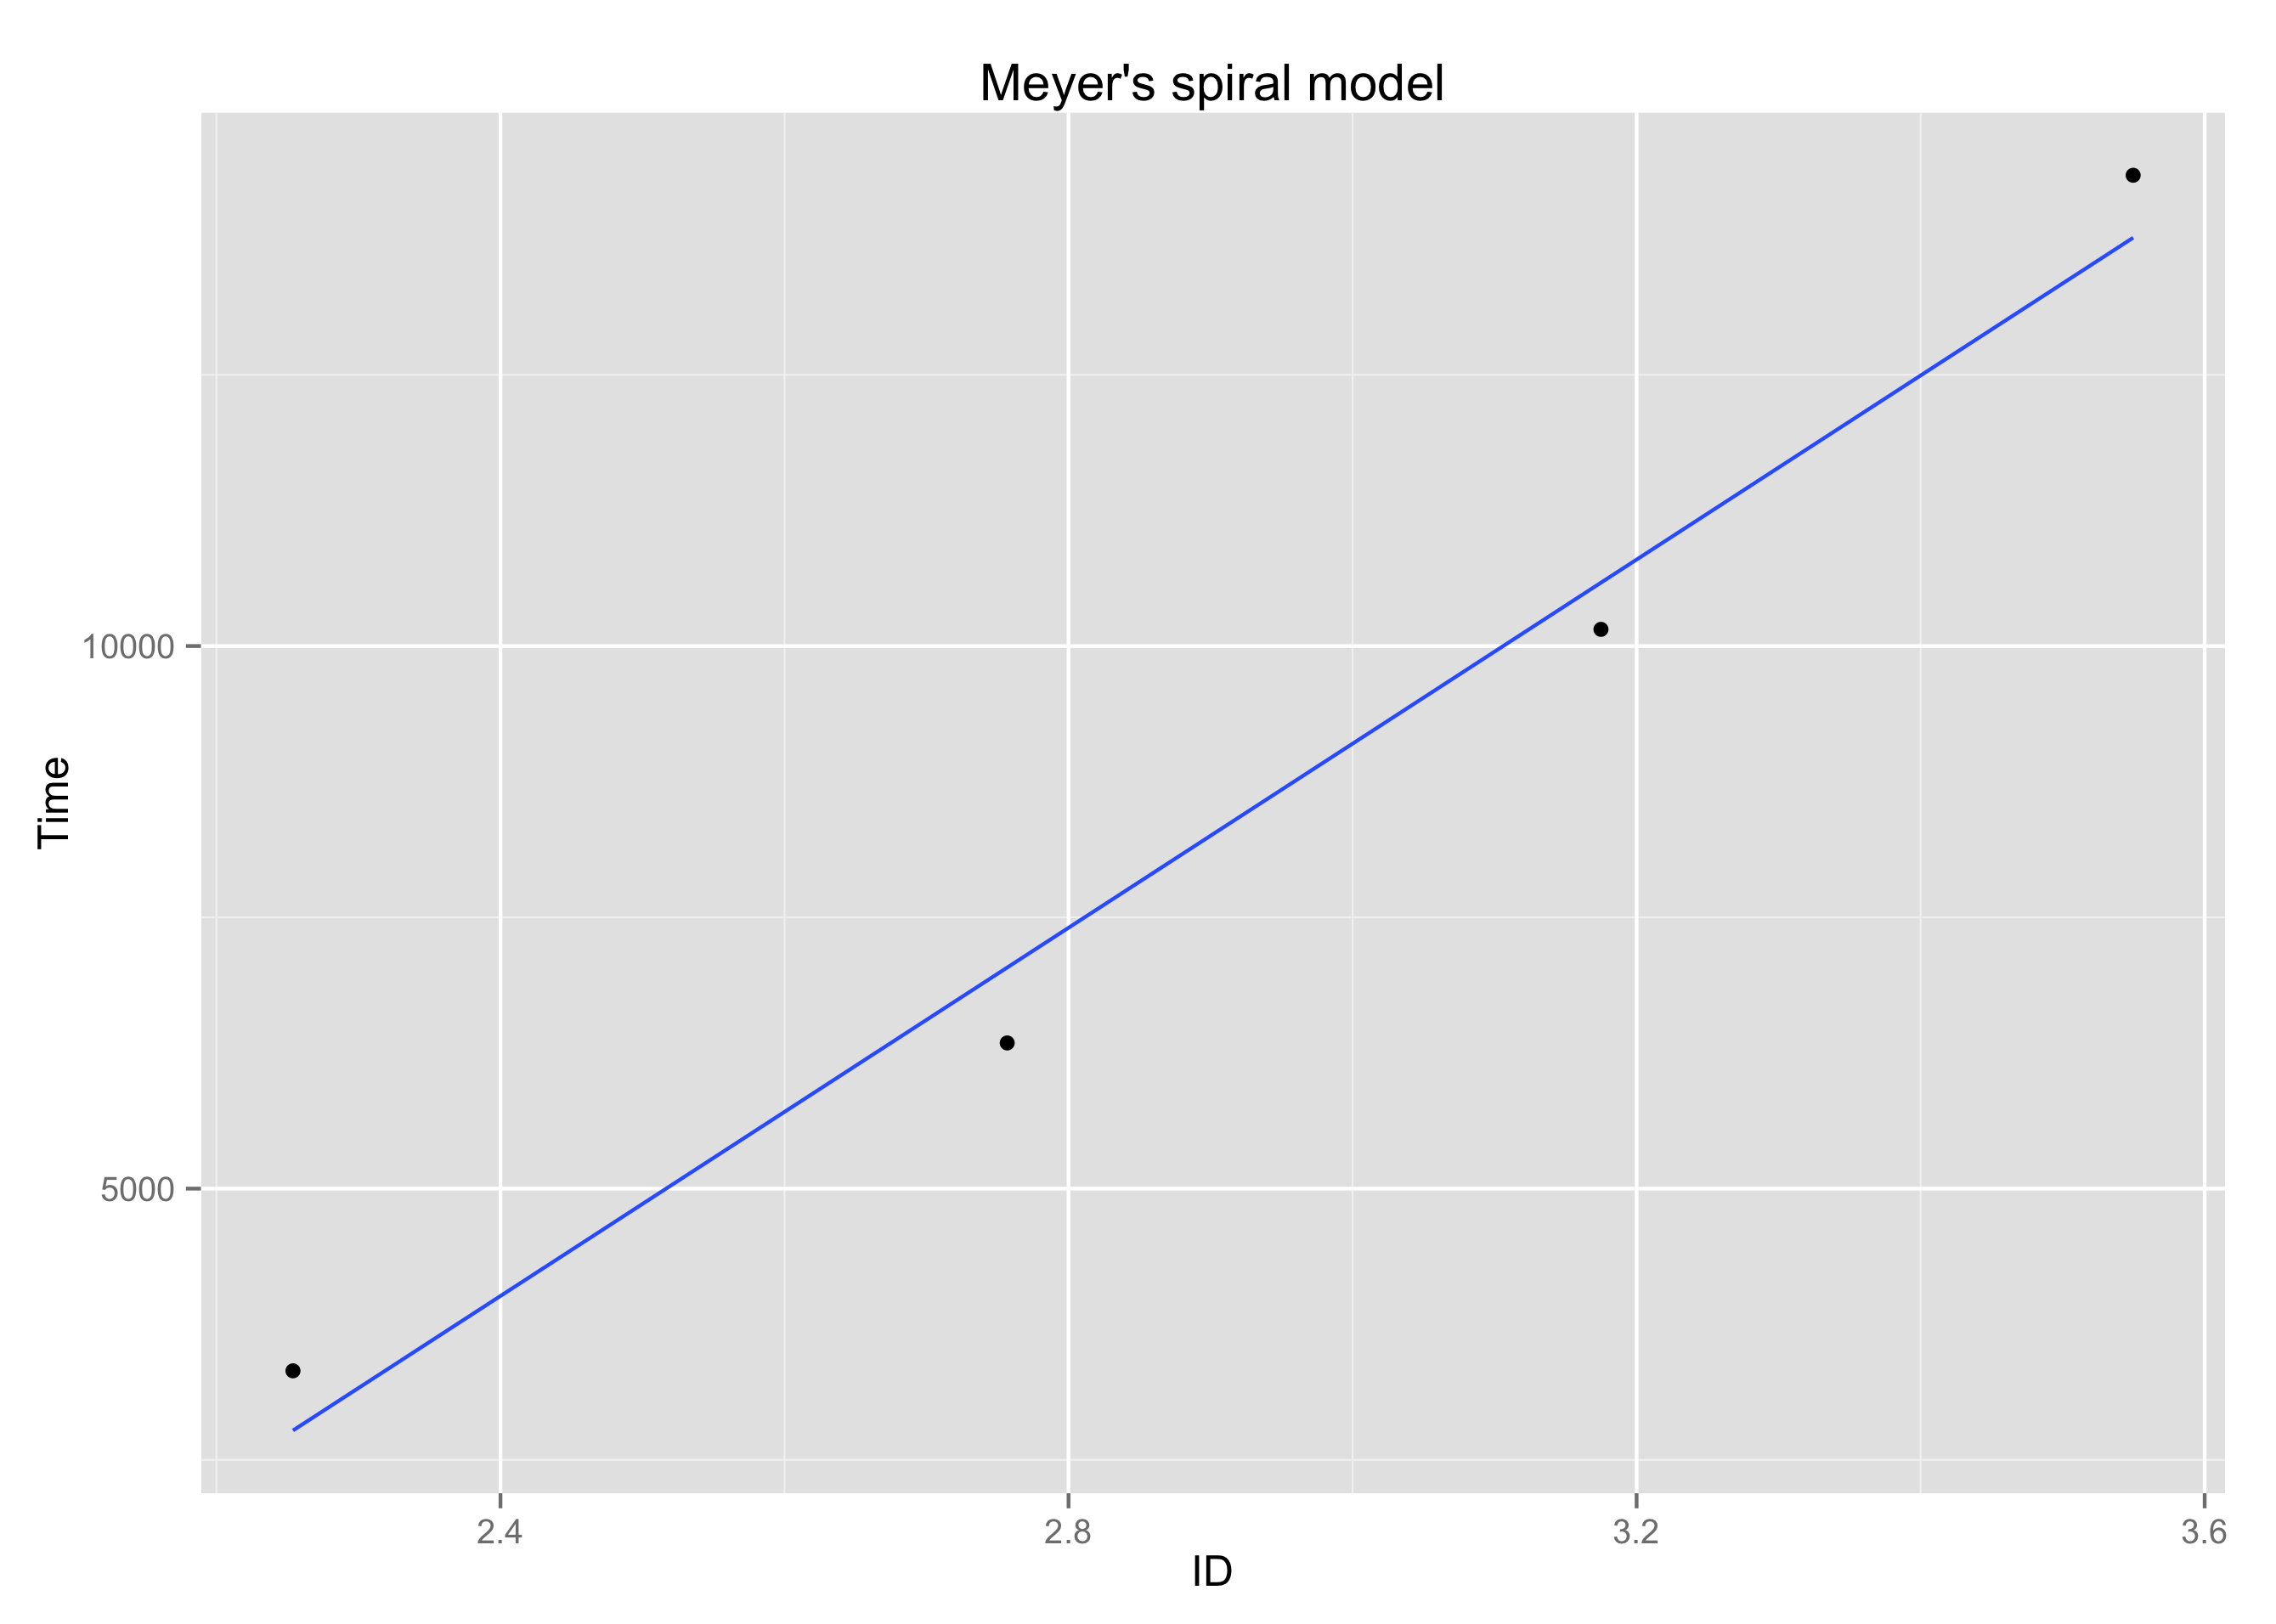
\includegraphics[width=\textwidth]{images/plots/plot_model_spiral_meyer}
		\captionof{figure}{Meyer's affine model til gennemsnitstiden per $ID$, med $ID$ på $x$-aksen og tiden $T$ på $y$-aksen}
		\label{fig:meyer_spiral_line}
	\end{minipage}
	\begin{minipage}[b]{0.1\linewidth}
	~
	\end{minipage}
	\begin{minipage}[t]{0.45\linewidth}
		\includegraphics[width=\textwidth]{images/plots/plot_model_spiral_mackenzie}
		\captionof{figure}{MacKenzie's affine model til gennemsnitstiden per $ID$, med $ID$ på $x$-aksen og tiden $T$ på $y$-aksen}
		\label{fig:mackenzie_spiral_line}
	\end{minipage}
\end{minipage}
\begin{minipage}{\linewidth}
	\begin{minipage}[t]{\linewidth}
		\centering
		\includegraphics[width=0.5\textwidth]{images/plots/plot_model_spiral_accot}
		\captionof{figure}{Accot \& Zhai's affine model til gennemsnitstiden per $ID$, med $ID$ på $x$-aksen og tiden $T$ på $y$-aksen}
		\label{fig:accot_spiral_line}
	\end{minipage}
\end{minipage}

\newpage
\addcontentsline{toc}{section}{modelanalyse af hastighedsprofiler}
\section*{Modelanalyse af hastighedsprofiler}
Vores modelanalyse af hastighedsprofiler tager udgangspunkt i en kvalitativ analyse. Vi vil gennemgå testdeltagernes bevægelsesbaner for pegeopgaverne, for at finde eventuelle tendenser, som vi kan opstille hypoteser ud fra. Hypoteserne vil vi forsøge, at be- eller afkræfte i en efterfølgende kvantitativ analyse.

\addcontentsline{toc}{subsection}{Kvalitativ analyse}
\subsection*{Kvalitativ analyse}
Den kvalitative analyse baserer sig på 22 tilfældigt udvalgte crowdsourcingdeltagere. De 22 testdeltagere er valgt med en tilfældighedsgenerator og har følgende id'er i databasen; $3,45,72,77,78,113,114,140$ $151,154,161,166,170,171,176,219,226,235,239,248,257,263$. Vi har plottet testdeltagernes bevægelsesbaner for alle deres pegeopgaver, hvilket gør det muligt at se sammenhænge imellem testdeltagerne. Figur \ref{fig:movement_random_person_1} og \ref{fig:movement_random_person_2} viser hvert ét eksempel på en testdeltagers bevægelsesbaner. De resterende 20 plots kan ses i bilag \ref{sec:movementlines}. Bevægelsesbaner med et højt $ID$ er mørkeblå, mens bevægelsesbaner med et lavt $ID$ er lyseblå.

Vi ser en tendens til, at testdeltagerne bruger én primær underbevægelse for at komme hen mod målet, efterfulgt af én eller flere korrigerende mindre underbevægelser for at ramme målet. Der er en tendens til, at bevægelser i opgaver med højere $ID$ vil have flere korrigerende underbevægelser end bevægelser i opgaver med lavere $ID$. 

Flere af testdeltagerne har også nogle få opgaver, hvor de kun har én primær underbevægelse uden nogen efterfølgende korrigerende bevægelser. Nogle testdeltagere har startet med at føre markøren i den forkerte retning og har derfor været nødt til at vende rundt og føre markøren i den rigtige retning, derved har de haft to større underbevægelser. Disse to observationer skal dog ikke ses som en generel tendens. Enkelte af testdeltagerne har haft opgaver, hvor de førte musen uden for canvas og disse baner er derfor ikke fuldendte.

På baggrund af de observerede tendenser har vi fundet frem til to hypoteser, som vi vil forsøge at få bekræftet. Den første hypotese er, at testdeltagerne bruger én primær underbevægelse til at bevæge markøren mod målet efterfulgt af én eller flere korrigerende underbevægelser for at ramme målet. Den anden hypotese er, at en opgave med højere $ID$ vil resultere i flere korrigerende underbevægelser.\\\\
\begin{minipage}{\linewidth}
	\begin{minipage}{.45\linewidth}
		\centering
		\includegraphics[width=\linewidth]{images/plots/plot_analysis_qualitative_140}
		\captionof{figure}{Plot over alle bevægelsesbaner lavet af testdeltager 140 under udførslen af denne deltagers pegeopgaver}
		\label{fig:movement_random_person_1}
	\end{minipage}
	\begin{minipage}[b]{0.1\linewidth}
	~
	\end{minipage}
	\begin{minipage}{.45\linewidth}
		\centering
		\includegraphics[width=\linewidth]{images/plots/plot_analysis_qualitative_248}
		\captionof{figure}{Plot over alle bevægelsesbaner lavet af testdeltager 248 under udførslen af denne deltagers pegeopgaver}
		\label{fig:movement_random_person_2}
	\end{minipage}
\end{minipage}

\addcontentsline{toc}{subsection}{Kvantitativ analyse}
\subsection*{Kvantitativ analyse}
For at finde ud af, om vores 22 tilfældigt udvalgte testpersoner er repræsentative for resten af testdeltagerne, har vi valgt at undersøge deres spørgeskemasvar. De procentvise fordelinger af grupperingerne i køn, pegeenhed med mere for alle testdeltagere, har vi udregnet og opstillet i tabel \ref{tab:persons_average}. Tilsvarende har vi gjort i tabel \ref{tab:sample_persons_average} med data fra vores 22 udvalgte testdeltagere. Ved sammenligning af dataene i de to tabeller, finder vi vores 22 testdeltagere repræsentative for vores datasæt.

\begin{table}[h]
	\centering
	\begin{tabular}{llllll}
		Alder           & Køn               & Computerspil              & Computere                 & Hånd                & Pegeenhed            \\\hline
		gns: \hfill24.5 & mand: \hfill88\%  & $<1$ time: \hfill24\%     & $<1$ time: \hfill2\%      & venstre: \hfill14\% & mus: \hfill61\%      \\
		min: \hfill13   & kvinde: \hfill9\% & $1-5$ timer: \hfill24\%   & $1-5$ timer: \hfill1\%    & højre: \hfill83\%   & touchpad: \hfill36\% \\
		max: \hfill62   & andet: \hfill3\%  & $5-15$ timer: \hfill27\%  & $5-15$ timer: \hfill2\%   & andet: \hfill3\%    & andet: \hfill3\%     \\
		                &                   & $15-40$ timer: \hfill22\% & $15-40$ timer: \hfill24\% &                     &\\
		                &                   & $>40$ timer: \hfill3\%    & $>40$ timer: \hfill71\%   &                     &
	\end{tabular}
	\caption{Tabel med oversigt over gennemsnitsværdier og fordeling af testdeltagerne valg i spørgeskemaet}
	\label{tab:persons_average}
\end{table}

\begin{table}[h]
	\centering
	\begin{tabular}{llllll}
		Alder            & Køn                  & Computerspil                & Computere                    & Hånd                   & Pegeenhed            \\\hline
		gns: \hfill24.9 & mand: \hfill91\%  & $<1$ time: \hfill18\%    & $<1$ time: \hfill0\%         & venstre: \hfill18\% & mus: \hfill50\%      \\
		min: \hfill17    & kvinde: \hfill9\% & $1-5$ timer: \hfill27\%  & $1-5$ timer: \hfill0\%       & højre: \hfill82\%   & touchpad: \hfill50\% \\
		max: \hfill41    &                      & $5-15$ timer: \hfill41\% & $5-15$ timer: \hfill0\%      &                        &                      \\
		                 &                      & $15-40$ timer: \hfill9\% & $15-40$ timer: \hfill32\% &                        &                      \\
		                 &                      & $>40$ timer: \hfill5\%   & $>40$ timer: \hfill68\%   &                        &
	\end{tabular}
	\caption{Tabel med oversigt over gennemsnitsværdier og fordeling af de 22 testdeltageres valg i spørgeskemaet}
	\label{tab:sample_persons_average}
\end{table}

For at undersøge vores hypoteser fra den kvalitative analyse har vi lavet fartprofiler for de 22 testdeltagere. Dette har vi gjort ved at udregne farten som forskellen i distancen over forskellen i tid; $\frac{\Delta \text{afstand}}{\Delta \text{tid}}$, hvilket er målt i pixels per millisekund. Vi har valgt at visualisere fartprofilerne for fire opgaver, hhv. $20,23,8$ og $22$, de er valgt fordi de har henholdvis de højeste og laveste $ID$ af vores 25 opgaver. $20$ og $23$ har de højeste værdier på $5.66$ og $5.54$, mens $8$ og $22$ har de laveste værdier på $1.94$ og $1.32$. Farten er visualiseret i forhold til den tilbagelagte afstand eller forløbne tid fra starten af opgaven. De to øverste plots illustrerer opgave $20$ og $23$ imens de to nederste illustrerer opgave $8$ og $22$.

Figur \ref{fig:speed_distance_testperson_140} og \ref{fig:speed_distance_testperson_248} er eksempler på farten i forhold til den tilbagelagte afstand, imens figur \ref{fig:speed_time_testperson_140} og \ref{fig:speed_time_testperson_248} er farten i forhold til den forløbne tid. Otte af de resterende plots kan ses i bilag \ref{sec:speed_plots}. Grunden til, at vi har valgt at medtage fartprofiler i forhold til både distance og tid er, at det giver os et mere nuanceret billede af, vores testpersoners bevægelse. Vi bemærker, hvordan graferne i figurerne generelt udviser en stigning fra starten af opgaven til et globalt maksimum, hvorefter farten aftager og nærmer sig 0. Dette er et tegn på én primær underbevægelse, da deltageren næsten stopper bevægelsen. Længden på denne underbevægelse varierer fra 40 til 300 pixels og farten ligger imellem 0 og 8 pixels per millisekund.

Grafen vil efter aftagningen foretage nul eller flere stigninger til lokale maksimum, som kan betegnes som korrigerende underbevægelser. Dette bekræfter derfor vores hypotese om, at testpersonerne har én primær underbevægelse efterfulgt af et antalt korrigerende underbevægelser, hvilket også er beskrevet tidligere i rapporten. Ydermere bemærker vi, at graferne for opgaver med højere $ID$ viser flere korrigerende underbevægelser end graferne for opgaver med lavere $ID$.

Som tidligere nævnt i rapporten, har de fire formuleringer af Fitts' lov et additivt led, som beskriver reaktionstiden for testdeltagerne. Disse værdier varierede fra 300 til 500 millisekunder, hvilket stemmer overens med graferne i figur \ref{fig:speed_time_testperson_140} og \ref{fig:speed_time_testperson_248}. Her starter deltagerne først efter 200 til 500 millisekunder. Bemærk, at grafen på nogle af figurerne allerede starter omkring tiden 0 og fortsætter med en fart på 0, dette skyldes, at testdeltageren har bevæget sin pegeenhed samtidig med, at deltageren klikkede for at starte opgaven. Derved er der blevet registreret et datapunkt, dog uden, at testdeltageren egentlig er startet med at manøvrere imod målet. Udover dette noterer vi os, at graferne udviser de samme egenskaber for både distance og tid.\\\\
\begin{minipage}{\linewidth}
\begin{minipage}{.475\linewidth}
	\centering
	\includegraphics[width=\linewidth]{images/plots/plot_speed_individual_140}
	\captionof{figure}{Plot af testdeltager 140's fart i forhold til den tilbagelagte distance på opgaverne 20, 23, 8 og 22}
	\label{fig:speed_distance_testperson_140}
	\end{minipage}
	\begin{minipage}[b]{0.05\linewidth}
	~
	\end{minipage}
	\begin{minipage}{.475\linewidth}
		\centering
		\includegraphics[width=\linewidth]{images/plots/plot_speed_individual_248}
		\captionof{figure}{Plot af testdeltager 248's fart i forhold til den tilbagelagte distance på opgaverne 20, 23, 8 og 22}
		\label{fig:speed_distance_testperson_248}
	\end{minipage}
\end{minipage}

\begin{minipage}{\linewidth}
\begin{minipage}{.475\linewidth}
	\centering
	\includegraphics[width=\linewidth]{images/plots/plot_speed_time_individual_140}
	\captionof{figure}{Plot af testdeltager 140's fart i forhold til den forløbne tid på opgaverne 20, 23, 8 og 22}
	\label{fig:speed_time_testperson_140}
	\end{minipage}
	\begin{minipage}[b]{0.05\linewidth}
	~
	\end{minipage}
	\begin{minipage}{.475\linewidth}
		\centering
		\includegraphics[width=\linewidth]{images/plots/plot_speed_time_individual_248}
		\captionof{figure}{Plot af testdeltager 248's fart i forhold til den forløbne tid på opgaverne 20, 23, 8 og 22}
		\label{fig:speed_time_testperson_248}
	\end{minipage}
\end{minipage}\\\\
Udover analyse af testdeltagernes fart, så har vi også valgt at lave hastighedsprofiler for fire opgaver for fire tilfældigt udvalgte personer. De fire opgaver er, ligesom fartprofilerne, opgave $20$, $23$, $8$ og $22$, da de har de laveste og højeste $ID$. Hastighedsprofilerne er lavet, både med retning mod næste punkt og med retning mod slutpunktet. Dette er gjort, for at se om der er en sammenhæng mellem hastigheden til næste punkt, eller målet, og tiden det tager at udføre en opgave. De 16 plots ses i bilag \ref{sec:velocity_plots}, mens figur \ref{fig:plot_velocity_individual} og \ref{fig:plot_velocity_individual_target} visualisere henholdsvis ét plot med hastighedsvektorer mod næste punkt og ét plot med hastighedsvektorer mod slutpunktet. Figur \ref{fig:plot_velocity_individual} og \ref{fig:plot_velocity_individual_target} er taget fra en tilfældig opgave fra en tilfældig testdeltager, udelukkende for at visualisere plots med pænere tendenser. 

Vektorerne i bilag \ref{sec:velocity_plots} udviser ingen generelle tendenser. Det ser ud til at være tilfældigt hvilke vektorer som er store og hvilke som er små. Derfor kan vi ikke se nogen sammenhæng mellem hastighedsprofiler og Fitts' lov.\\\\
\begin{minipage}{\linewidth}
	\begin{minipage}{.45\linewidth}
		\includegraphics[width=\linewidth, trim = 20cm 0cm 20cm 0cm, clip]{images/plots/plot_velocity_individual}
		\captionof{figure}{Vektorplot over hastighedsprofilen for en tilfældig testdeltager}
		\label{fig:plot_velocity_individual}
	\end{minipage}
	\begin{minipage}[b]{0.1\linewidth}
	~
	\end{minipage}
	\begin{minipage}{.45\linewidth}
		\includegraphics[width=\linewidth, trim = 20cm 0cm 20cm 0cm, clip]{images/plots/plot_velocity_individual_target}
		\captionof{figure}{Vektorplot over hastighedsprofilen mod målet for en tilfældig testdeltager}
		\label{fig:plot_velocity_individual_target}
	\end{minipage}
\end{minipage}


\addcontentsline{toc}{chapter}{Diskussion}
\chapter*{Diskussion}
Vi vil i dette afsnit diskutere vores fremgangsmåde og resultater fra både vores forsøgsopstilling og analyse.

\addcontentsline{toc}{section}{Forsøgsopstilling}
\section*{Forsøgsopstilling}

\begin{wrapfigure}{r}{.45\linewidth}
	\centering
	\begin{tabular}{ll}
		\textbf{Fordele} & \textbf{Ulemper}\\\hline
		Flere deltagere & Lavere feedbackkvalitet\\
		Hurtigere & Mindre interaktion\\
		Lavere omkostninger & Spammere\\
		Forskellige baggrunde & Store målgrupper\\
	\end{tabular}
	\caption{Tabel med oversigt over fordele og ulemper ved brug af crowdsourcing i forhold til laboratorieforsøg \cite{liu2012crowdsourcing}}
	\label{tab:fordeleogulemper}
\end{wrapfigure}

Vi valgte at opdele vores forsøg i to dele; et kontrolleret laboratorieeksperiment, og et ukontrolleret crowdsourcingeksperiment. Opdelingen blev lavet for at sikre, at vi havde nogle kontrollerede data som vi kunne bruge til at måle kvaliteten af vores ukontrollerede data med. Ifølge \cite{liu2012crowdsourcing} er der fordele ved både laboratorieforsøg, og ved crowdsourcing - disse ses i tabel \ref{tab:fordeleogulemper} som illustrerer det fra et crowdsourcing perspektiv. Den lavere kvalitet af feedback, og den manglende interaktion med deltagerne fremhæver vigtigheden af at udføre et laboratorieeksperiment, hvor disse problemer netop ikke vil være til stede \cite{liu2012crowdsourcing}. Det kan derfor diskuteres om vores 10 testdeltagere til det kontrollerede laboratorieforsøg er tilstrækkeligt, eller om vi burde have haft en større mængde deltagere, og sikret os en større mængde data af højere kvalitet. Derudover ville det også have givet os en mulighed for at finde flere folk fra en mere varieret målgruppe, til at sammenligne crowdsourcingdata med.

Fordelene ved at bruge crowdsourcing taler dog klart for også at gøre brug af dette. Dog bliver der refereret til services som Amazon Mechanical Turk og CrowdFlower \cite{liu2012crowdsourcing}, der begge er betalingsservices, hvilket har nogle andre fordele og ulemper end vores valg af frivillige testdeltagere. De lave omkostninger, og den hurtige udførsel taler for at vælge betalingsservices, og ville have sikret os en større mængde data. Men vi kan ikke sige om kvaliteten af data havde været bedre, da der ved betalt crowdsourcing bliver et incitament til at gennemføre opgaverne hurtigere grundet Amazon Mechanical Turks betaling per gennemført opgave \cite{liu2012crowdsourcing}.

Vores valg af opslagssteder til det ukontrollerede forsøg kan have haft en indflydelse på den indsamlede data. Vi valgte at bruge Reddit, hvilket giver os en meget specifik målgruppe, da den typiske Reddit-bruger er mand imellem 18 og 29 år\footnote{\href{http://www.pewinternet.org/2013/07/03/6-of-online-adults-are-reddit-users/}, besøgt: 03-06-2015}. Dette er også udslagsgivende i vores indsamlede data, hvor gennemsnitsalderen er 24.5 år og 233 ud af 257 er mænd.

Vores testdata kom ikke kun fra Reddit, men også fra opslag på vores Facebook-væg. Dette medfører også et bias som kan være væsentligt, da det er vores familie og venner vi derved bruger. Familie og venner har ofte hørt om projektet før og kan derfor have en forventning om hvad der skal ske og hvad de burde gøre. Da både Reddit og Facebook hovedsageligt bruges af yngre personer, vil vores målgruppe også være begrænset heraf. Vi har for eksempel kun ni testpersoner, som er ældre end 40. Hvis vi skulle undgå dette ville vi være nødt til at lave flere kontrollerede forsøg med aldersgrænse for testdeltagerne, eller bruge crowdsourcing sider, der henvender sig til den ældre befolkningsgruppe.

\begin{wrapfigure}{l}{.40\linewidth}
	\centering
	\begin{tabular}{ll}
		\textbf{Computerspil} & \textbf{Gennemsnitstid}\\\hline
		$<1$ time    & 1052.307ms\\
		1-5 timer    & 1008.317ms\\
		5-15 timer   & 963.7545ms\\
		15-40 timer  & 917.7642ms\\
		$>40$ timer  & 896.4097ms\\
	\end{tabular}
	\caption{Tabel med oversigt over testpersoners spilletid, sammenlignet med deres gennemsnitlige gennemførselshastighed af pegeopgaverne}
	\label{tab:times_average}
\end{wrapfigure}

Det er førhen blevet påvist, at folk der spiller computer vil være hurtigere \cite{wyeld2013}. I vores undersøgelse er dette også tilfældet, da tabel \ref{tab:times_average} viser at gennemsnitstiderne for at gennemføre en opgave falder desto mere computer deltageren spiller.

Ligeledes kan der være en væsentlig forskel på tiden, alt efter om testpersonen bruger mus eller touchpad \cite{epps1986}. I vores data brugte 160 testdeltagere mus, imens 96 brugte touchpad. I følge \cite{epps1986} ville dette betyde en forskel i de indbyrdes tider og derved også mindre sammenhæng i dataene. Dette kan medføre et dårligere resultat når vi forsøger at tilpasse vores modeller til hele datasættet. Det kunne derfor have været relevant at foretage en analyse af hhv. mus og touchpad brugere, hver for sig.

\addcontentsline{toc}{section}{Analyse}
\section*{Analyse}
% Diskussion af AIC
Analysen af pegeopgaverne viste, at Meyer's formulering beskrev vores indsamlede data bedst, da den havde en AIC-værdi på 92728.38 for alle personers pegeopgaver. Dette var 34.64 mindre end AIC-værdien for MacKenzie's formulering, som viste sig at være den næstbedste formulering. Herefter fulgte AIC-værdien for Fitts' formulering som var 75.79 større end selvsamme for Meyer's formulering. Den formulering som passede vores data dårligst var Welford's, den havde den højeste AIC-værdi og var 1781.96 større end selvsamme for Meyer's formulering. For at kunne sige, at to modeller passer den indsamlede data lige godt, så skal forskellen mellem dem være under to \cite{burnham2004}. Hvis de måske passer den indsamlede data lige godt, så skal forskellen mellem dem være mellem fire og syv \cite{burnham2004}. Hvis de ikke passer dataen lige godt, så vil forskellen ligge over 10 \cite{burnham2004}. Forskellene mellem Meyer's formulering og de tre andre er alle større end 10. Vi kan derfor sige at Meyer's er den formulering som passer vores data bedst, da den har den mindste AIC-værdi.

Vi valgte også at lave AIC-analyse af alle opgaver for 10 tilfældige personer. Her var resultaterne mere varierede, men Meyer's formulering havde den laveste AIC-værdi ved syv ud af de 10 testdeltagere. MacKenzie's formulering havde den laveste ved to ud af de 10 testdeltagere, mens Welford's formulering havde den laveste værdi ved en af testdeltagerne. Der var en generel tendens til at forskellene mellem Meyer's formulering, MacKenzie's formulering og Fitts' formulering lå under to, hvilket betyder at de passer lige godt for dataen for enkeltpersoner. Welford's var lidt mere blandet. Her var en af forskellene under to, seks var mellem to og 10 og to var over 10. Det tyder altså på at Welford's formulering på enkeltpersonerne måske passer lige så godt på dataen som de fire andre, men at vi ikke kan være sikre på dette.

For at understøtte vores AIC-analyse lavede vi også en analyse af residualplots. På residualplottene var det tydeligt at se at Meyer's formulering var den som passede bedst på den indsamlede data, da dens smoothing-linje generelt var nærmest nul-linjen og dens residualer lå mest tilfældigt omkring nul-linjen. MacKenzie's og Fitts' formulering lignede hinanden rigtig meget og vi kan derfor ikke se hvilken af dem der vil være næst- og tredjebedst. Det er dog klart ud fra residualplottene, at Welfold's formulering er den som passer dårligst på dataen, da smoothing-linjen ligger længere fra nul-linjen og residualplottene ikke ligger tilfældigt omkring nul-linjen. Residualplottene følger altså vores AIC-analyse, idet Meyer's formulering er den bedste og Welford's er den dårligste. Det er dog svært at sige om Fitts' og MacKenzie's formulering ligger tæt nok på Meyer's til at de passer lige så godt på dataen, hvilket vores AIC-analyse til gengæld klart kunne svare på at de ikke gjorde for alle deltagere.

I vores analyse fandt vi frem til værdien af $a$ og $b$ i hver af de fire formuleringer for alle testpersoners pegeopgaver. De tre værdier af $a$ beskriver den tid det vil tage for en person at påbegynde opgaven. Denne ligger mellem cirka $400$ og $500$ millisekunder, hvilket også passer med hvad \cite{crossman1957} og \cite{welford1968} tidligere har fundet frem til. Det multiplikative led, $b$, beskriver hvor meget længere tid brugeren ville bruge på en opgave, hvis opgavens $ID$ bliver 1 større. Dette led ligger for Fitts', MacKenzie's og Meyer's omkring $150-200$, mens det for Welford's ligger omkring $300$. Grunden til at Welford's multiplikative led ligger højere er, at Welford's formulering ikke har det additive led og derfor vil den skulle stige mere, for at passe nogenlunde på vores data.

Da vores pegeopgaver er en reproducering af tidligere udførte forsøg i \cite{goldberg2015}, så vil vi sammenligne vores resultater med deres. Vi fandt, i vores analyse, at Meyer's formulering var den, som tilpassede vores data bedst, ved alle testdeltageres pegeopgaver. \cite{goldberg2015} fandt frem til, at MacKenzie's formulering er den som generelt tilpasser deres data bedst. Vi har derfor ikke kunne reproducere resultaterne som de fandt frem til i \cite{goldberg2015}, på trods af, at vi har reproduceret deres pegeopgave. Der kan derfor stilles spørgsmålstegn ved rigtigheden af resultaterne i \cite{goldberg2015}.

% Fart diskussion
Teorien om én primære underbevægelse efterfulgt af korrigerende underbevægelser, er som tidligere beskrevet, bekræftet af vores data. Selvom fartprofilerne vist i figur \ref{fig:speed_distance_testperson_140}-\ref{fig_speed_time_testperson_248} ikke har de samme afrundede og tydeligt distinkte kurver som \ref{fig:CrossmanFitt}, så stemmer vores data overens med Crossman og Goodeve's forklaring i \cite{crossman1983}. Vi har ydermere vist at fartprofilerne ofte udviser en eller flere korrigerende underbevægelser, hvilket også stemmer overens med \cite{crossman1983}. I modsætning hertil, så udviser hastighedsvektorerne ingen generelle tendenser og vi har ikke kunne bruge vektordataen til at beskrive eller forbedre Fitts' lov.

% Diskussion af tunnel
I vores analyse af tunnelopgaverne viste tabel \ref{tab:table_analysis_aic_tunnel_all} og \ref{tab:table_analysis_aic_tunnel_mean} at Meyer's formulering, da den havde den mindste AIC-værdi, på hhv. $20549.61$ og $33.68$. Det var dog ikke entydigt hvilken af formuleringerne som tilpassede dataen bedst, da både Accot \& Zhai's, MacKenzie's og Fitts' formulering havde AIC-værdier, hvor forskellen var under to. Derfor kan vi kun sige at de alle tilpasser dataen lige godt. Ved AIC-værdierne for gennemsnitstiderne er forskellen i mellem formuleringerne markant højere. Kun Accot \& Zhai's formulering har en forskel, der er mindre end 10, hvilket betyder, at de tre andre formuleringer ikke kan beskrive vores data i samme grad. Vores analyse viste også at Welford's formulering var den som beskrev vores data dårligst, da den havde den højeste AIC-værdi og forskellen var lige under ni. Vi kan altså ikke helt udelukke Welford's formulering og kan heller ikke sige hvilken formulering som beskriver vores data bedst.

På forhånd havde vi forventet, at det ville være Accot og Zhai's formulering, som beskrev vores data bedst. Dette er dog ikke entydigt tilfældet, selvom de fire andre formuleringer ikke er beregnet til denne type opgaver. Dette kan skyldes flere ting, men specielt er det vigtigt at notere sig, at vores data til tunnelopgaverne ikke nødvendigvis er repræsentative. Vi har flere eksempler på personer, som fik bedre tider desto større $ID$, et eksempel herpå kan ses i figur \ref{fig:navigationtest2}. I forhold til \cite{accot1997} så har vi kun haft fire tunnelopgaver, mens de brugte 16. Dette fører til, at vi har et væsentlig mindre span af $ID$ og væsentlig mindre data at basere vores analyse på. Det er med til at gøre vores konklusion om tunnelopgaverne mindre pålidelige.

I forhold til Accot og Zhai så er der også stor forskel i vores modellers konstanter $a$ og $b$. De fandt frem til $a=-532$ og $b=93$, imens vores tilsvarende konstanter er $a=6112.4$ og $b=47.77$, forskellen skyldes formentligt antallet af opgaver og derved også antallet af forskellige $ID$, men derudover så burde vores forsøg være ens. Deres værdier er fra tilpasning til gennemsnitstiderne imens vores er til det fulde datasæt, vi har dog også fundet konstanterne til gennemsnitstiderne for vores datasæt, hvilket gav $a=6112.7$ og $b=47.77$, som er næsten identisk med vores allerede beskrevne værdier.

\cite{accot1997} bruger gennemsnitstiderne til at udføre deres udregninger, hvilket vi har valgt ikke at gøre. Hvis vi havde valgt at gøre det, ville vi have haft fire datapunkter for tunnelopgaverne, hvilket er så få at $AIC$ ikke er beregnet til at sammenligne modellerne. I dette tilfælde kunne vi have brugt $AIC_c$, som er beregnet til at beregne AIC-værdier for datasæt, hvor antallet af datapunkter, $n$, er tilpas lille. Burnham argumenter i \cite{burnham2004} for, at hvis $\frac{n}{K} <\approx 40$ så bør $AIC_c$ bruges i stedet for $AIC$, i vores tilfælde har vi $n=4$ og $K=2 \vee 1$, hvilket giver værdier markant mindre end 40. Vi har dog valgt ikke at bruge $AIC_c$, men derimod gøre brug af hele vores datasæt.

% Diskussion af spiral
Modsat vores tunnelopgave analyse så viste spiralopgaverne store forskelle i mellem AIC-værdierne, vist i tabel \ref{tab:table_analysis_aic_spiral_all} og \ref{tab:table_analysis_aic_spiral_mean}. Accot og Zhai's formulering beskrev vores data bedst med AIC-værdier på $20225.67$ og $61.91$ for hhv. det fulde datasæt og gennemsnitstiderne. De indbyrdes 'placeringer' er ens for begge AIC-analyser, men ligesom for tunnelopgaverne så er der en væsentlig variation i forskellene. Vi vil dog tage udgangspunkt i AIC-analysen for det fulde datasæt, på baggrund af samme argument som for navigationsopgaverne.

Alle forskellene i tabel \ref{tab:table_analysis_aic_spiral_all} er større end 10, og vi kan derfor konkludere, at Accot og Zhai's formulering beskriver vores data bedre end de fire andre formuleringer. Dette er præcis, hvad vi forventede, da deres $ID$ er bestemt specifikt for denne type opgave. Ligesom for tunnelopgaverne gjorde vi kun brug af 4 i stedet for 16 opgaver, hvilket gør datasættet væsentligt mindre og måske endda for lille. I modsætning til tunnelopgaverne så har spiralopgavernes størrelser mere indflydelse på tiden. Hvis spiralen bliver større eller snævrere tager det længere tid for alle testdeltagerene at gennemføre. Sammenligningen med de fire originale formuleringer af Fitts' lov er dog svær at drage yderligere konklusioner ud fra. De motoriske analyser som de bygger på, med én hovedbevægelse efterfulgt af én eller flere underbevægelser er formentligt ikke tilfældet for spiralopgaven.

I forhold til vores konstanter $a$ og $b$ og Accot og Zhai's, så er der igen en væsentlig forskel, de fik $a=115$ og $b=169$, imens vores værdier er på $a=2097.09$ og $b=553.25$. Det er svært at diskutere i yderlighed, hvad denne forskel betyder, da vi kun har brugt 4 spiralopgaver imens de brugte 16, og endvidere har vi heller ikke brugt den samme værdi, $w$, for bredden af spiraltunnellerne, dette skyldes, at vi ikke fik vores programmel til at tegne spiraller ved hjælp af polære koordinater ligesom Accot og Zhai har gjort det.

\addcontentsline{toc}{chapter}{Konklusion}
\chapter*{Konklusion}
Vi har redegjort for Fitts' lov og gennemgået tre alternative formuleringer af samme lov. Vi har på baggrund af et kontrolleret og ukontrolleret eksperiment reproduceret tidligere udførte forsøg og indsamlet data fra i alt 274 testdeltagere. Dataene har vi analyseret kvalitativt og kvantitativt, ved at kigge på grafer, tilpasse lineære modeller og sammenligne disse ved AIC- og residual-analyse. 

Vi kan på baggrund af denne analyse konkludere, at Meyer's formulering beskriver vores data fra pegeopgaverne bedst, derudover konkluderer vi, at formuleringerne beskriver vores tunnelopgavedata lige godt og, at det derfor er indifferent, hvilken variation man bruger til vores data. Ydermere kan vi konkluderer, at Accot og Zhai's formulering er bedst til at beskrive spiralopgavedata. Til sidst kan vi konkludere, at Welford's formulering klarer sig dårligst i at beskrive alle vores tre forskellige typer opgaver.

\addcontentsline{toc}{section}{Fremtidigt arbejde}
\section*{Fremtidigt arbejde}
Ved videre udarbejdelse af projektet, kunne det have været interessant at foretage en mere dybdegående analyse af hastighedsprofilerne. Ved at studere flere af testdeltagernes tilhørende vektorplots kunne der have været større grobund for at se en sammenhæng imellem dem og Fitts' lov. Endvidere ville vi gerne have haft mulighed for at sammenligne testdeltagernes tider i forhold til flere af deres spørgeskemasvar, såsom forskel på mænd og kvinder, højre eller venstre hånd og så videre.

I forhold til tunnel og spiralopgaverne ville det være naturligt at tilføje flere af denne type opgaver, for bedre at kunne undersøge om Accot og Zhai's formuleringer rent faktisk stemmer bedre overens med denne type opgaver i forhold til Fitts' lov. Hertil kunne man også godt kigge på fart og hastighedsprofiler. Blandt andet formoder vi, at navigationsopgaver har flere primære underbevægelser i stedet for kun én, hvilket går imod teorien bag de klassiske formuleringer af Fitts' lov.

Med den teknologiske udvikling kunne det også være relevant at undersøge Fitts' lov i forhold til skærme med 'motion sensors'. Nærmere betegnet om forholdet imellem tiden det tager at udføre opgaven og sværhedsgraden af opgaven er det samme når man er fri for at bruge en pegeenhed eller røre ved skærmen.

%\textbf{Konklusionen er afslutningen på din akademiske opgave. Her fortæller du din læser hvad du har fundet ud af i din undersøgelse/analyse, og hvorfor det er vigtigt.}
%Konklusionen kan indeholde:
%\begin{itemize}
%	\item opgavens hovedpunkter og resultater i kort form
%	\item svar på problemformuleringen
%	\item vurdering af metode i form af en nuancering og evaluering af din fremgangsmåde
%	\item perspektivering af emnet – hvis der er basis for det
%\end{itemize}

\nocite{*}
\begin{appendices}

%-- Drejebog --%
\chapter{Drejebog for laboratorieeksperiment}
\label{sec:drejebog}
\subsection*{Udstyr}
\begin{itemize}
\item{Computer med Google Chrome browseren}
\item{Mus og musemåtte}
\end{itemize}
\subsection*{Før test}
\begin{itemize}
\item{P1 rækker testdeltager et A4 ark med følgende tekst;
      \\\textit{"Vi er i gang med et bachelorprojekt, der handler om Fitts' lov. Det er en model, som beskriver det menneskelige motoriske systems kapacitet. I denne sammenhæng, hvordan tiden til at ramme et mål på skærmen ved hjælp af musen afhænger af afstanden til og størrelsen på målet. Vi har derfor udviklet dette eksperiment for at indsamle data. Du vil undervejs blive stillet forskellige opgaver, som du skal forsøge at løse."}}
\item{P1 beder testdeltageren om at teste musens følsomhed ved at køre frit rundt med musen. Der gøres opmærksom på, at testdeltageren gerne må ændre følsomheden, hvis de føler for det.}
\item{P2 starter en Google Chrome browser og peger den på følgende adresse:\\ \url{http://codeit.io/bachelor/survey.html}.}
\end{itemize}
\subsection*{Under test}
\begin{itemize}
\item{P2 beder testdeltageren om at tage plads ved den klargjorte computer.}
\item{P2 beder testdeltageren om at udfylde formularen på skærmen med information.}
\item{P2 gør opmærksom på, at der skal skrives 'testperson x', hvor 'x' er nummeret på testpersonen, i feltet om hvorfra de hørte om siden (dette er for senere at kunne finde dem i databasen)}
\item{P1 fortæller testdeltageren, at de gerne må gå i gang med opgaverne og kan stille spørgsmål undervejs, hvis de har brug for det.}
\end{itemize}
\subsection*{Efter test}
\begin{itemize}
\item{P1 fortæller testdeltageren, hvordan  deres data vil blive brugt;
\\\textit{"Tak fordi du ville deltage i forsøget og hjælpe os med vores projekt. De baner du undervejs har foretaget for at udføre opgaverne vil blive brugt til at analysere, hvorvidt de stemmer overens med forskellige formuleringer af Fitt's lov, eller om der kan findes en forbedret formulering"}.}
\end{itemize}

%-- Tekst til crowdsourcing --%
\chapter{Tekst til crowdsourcing}
\label{sec:crowdsource-text}
For at crowdsource vores eksperiment har vi delt følgende tekst:
\\\\\textit{"Hej,\\ vi er tre datalogi studerende ved Københavns Universitet, som er i gang med vores bacheloropgave. For at kunne have nogle data at analysere, har vi lavet denne hjemmeside med 'pegeopgaver'. Opgaverne tager cirka 10-15 minutter at udføre og er skidesjove! Det ville derfor være utrolig værdsat, hvis du ville gå ind på følgende hjemmeside \url{http://www.codeit.io/bachelor/index.html} og udføre opgaverne. Deltag senest d. 27/04.
\\Eventulle spørgsmål kan henvendes til en af os på;\\bdj816@alumni.ku.dk, hmd200@alumni.ku.dk, qgf142@alumni.ku.dk"}
\\\\\textit{"Hello,\\ We are three computer science students at the University of Copenhagen, who are currently working on our bachelor thesis. We have made the following webpage with 'pointingtasks' in order to have some data to analyze. The tasks takes approximately 10-15 minuttes and are super fun! It would therefore be very appreciated if you would visit the webpage at \url{http://www.codeit.io/bachelor/index.html} and complete the tasks. Deadline is the 27th of April.
\\Any questions regarding the projects are welcome at either of these emails;\\bdj816@alumni.ku.dk, hmd200@alumni.ku.dk, qgf142@alumni.ku.dk"}

%-- Skærmbilleder af eksperiment --%
\chapter{Skærmbilleder af eksperiment}
\label{sec:screenshots}
\begin{minipage}{\textwidth}
\centering
\includegraphics[width=\textwidth]{images/screenshots/ex_step_1_intro}
\captionof{figure}{Eksperiment - Trin 1 - Intro}
\label{fig:ex_step_1_intro}
\includegraphics[width=\textwidth]{images/screenshots/ex_step_2_consent}
\captionof{figure}{Eksperiment - Trin 2 - Samtykke}
\label{fig:ex_step_2_consent}
\end{minipage}

\begin{minipage}{\textwidth}
\centering
\includegraphics[width=\textwidth]{images/screenshots/ex_step_3_questions}
\captionof{figure}{Eksperiment - Trin 3 - Spørgsmål}
\label{fig:ex_step_3_questions}
\end{minipage}

\begin{minipage}{\textwidth}
\centering
\includegraphics[width=\textwidth]{images/screenshots/ex_step_4_tunnel_1}
\captionof{figure}{Eksperiment - Trin 4 - Tunnel 1}
\label{fig:ex_step_4_tunnel_1}
\includegraphics[width=\textwidth]{images/screenshots/ex_step_4_tunnel_2}
\captionof{figure}{Eksperiment - Trin 4 - Tunnel 2}
\label{fig:ex_step_4_tunnel_2}
\end{minipage}

\begin{minipage}{\textwidth}
\centering
\includegraphics[width=\textwidth]{images/screenshots/ex_step_4_tunnel_3}
\captionof{figure}{Eksperiment - Trin 4 - Tunnel 3}
\label{fig:ex_step_4_tunnel_3}
\includegraphics[width=\textwidth]{images/screenshots/ex_step_4_tunnel_4}
\captionof{figure}{Eksperiment - Trin 4 - Tunnel 4}
\label{fig:ex_step_4_tunnel_3}
\end{minipage}

\begin{minipage}{\textwidth}
\centering
\includegraphics[width=\textwidth]{images/screenshots/ex_step_4_tunnel_path}
\captionof{figure}{Eksperiment - Trin 4 - Tunnelbane}
\label{fig:ex_step_4_tunnel_path}
\includegraphics[width=\textwidth]{images/screenshots/ex_step_4_tunnel_next}
\captionof{figure}{Eksperiment - Trin 4 - Næste tunnel}
\label{fig:ex_step_4_tunnel_next}
\end{minipage}

\begin{minipage}{\textwidth}
\centering
\includegraphics[width=\textwidth]{images/screenshots/ex_step_4_tunnel_done}
\captionof{figure}{Eksperiment - Trin 4 - Fortsæt}
\label{fig:ex_step_4_tunnel_done}
\includegraphics[width=\textwidth]{images/screenshots/ex_step_5_spiral_1}
\captionof{figure}{Eksperiment - Trin 5 - Spiral 1}
\label{fig:ex_step_5_spiral_1}
\end{minipage}

\begin{minipage}{\textwidth}
\centering
\includegraphics[width=\textwidth]{images/screenshots/ex_step_5_spiral_2}
\captionof{figure}{Eksperiment - Trin 5 - Spiral 2}
\label{fig:ex_step_5_spiral_2}
\includegraphics[width=\textwidth]{images/screenshots/ex_step_5_spiral_3}
\captionof{figure}{Eksperiment - Trin 5 - Spiral 3}
\label{fig:ex_step_5_spiral_3}
\end{minipage}

\begin{minipage}{\textwidth}
\centering
\includegraphics[width=\textwidth]{images/screenshots/ex_step_5_spiral_4}
\captionof{figure}{Eksperiment - Trin 5 - Spiral 4}
\label{fig:ex_step_5_spiral_4}
\includegraphics[width=\textwidth]{images/screenshots/ex_step_5_spiral_path}
\captionof{figure}{Eksperiment - Trin 5 - Spiralbane}
\label{fig:ex_step_5_spiral_path}
\end{minipage}

\begin{minipage}{\textwidth}
\centering
\includegraphics[width=\textwidth]{images/screenshots/ex_step_5_spiral_next}
\captionof{figure}{Eksperiment - Trin 5 - Næste spiral}
\label{fig:ex_step_5_spiral_next}
\includegraphics[width=\textwidth]{images/screenshots/ex_step_5_spiral_done}
\captionof{figure}{Eksperiment - Trin 5 - Fortsæt}
\label{fig:ex_step_5_spiral_done}
\end{minipage}

\begin{minipage}{\textwidth}
\centering
\includegraphics[height=.4\textheight]{images/screenshots/ex_step_6_pointing_start}
\captionof{figure}{Eksperiment - Trin 6 - Start}
\label{fig:ex_step_6_pointing_start}
\includegraphics[height=.4\textheight]{images/screenshots/ex_step_6_pointing_target_1}
\captionof{figure}{Eksperiment - Trin 6 - Pegeeksempel 1}
\label{fig:ex_step_6_pointing_target_1}
\end{minipage}

\begin{minipage}{\textwidth}
\centering
\includegraphics[height=.4\textheight]{images/screenshots/ex_step_6_pointing_target_2}
\captionof{figure}{Eksperiment - Trin 6 - Pegeeksempel 2}
\label{fig:ex_step_6_pointing_target_2}
\includegraphics[height=.4\textheight]{images/screenshots/ex_step_6_pointing_path}
\captionof{figure}{Eksperiment - Trin 6 - Pegebane}
\label{fig:ex_step_6_pointing_path}
\end{minipage}

\begin{minipage}{\textwidth}
\centering
\includegraphics[height=.4\textheight]{images/screenshots/ex_step_6_pointing_done}
\captionof{figure}{Eksperiment - Trin 6 - Færdig}
\label{fig:ex_step_6_pointing_done}
\includegraphics[height=.4\textheight]{images/screenshots/ex_step_7_sending}
\captionof{figure}{Eksperiment - Trin 7 - Sender}
\label{fig:ex_step_7_sending}
\end{minipage}

%-- Kvalitativ analyse --%
\newpage
\chapter{Testdeltageres bevægelsesbaner}
\label{sec:movementlines}
\begin{minipage}{\textwidth}
	\begin{minipage}{0.5\linewidth}
		\includegraphics[width=\linewidth]{images/plots/plot_analysis_qualitative_77}
	\end{minipage}
	\begin{minipage}{0.5\linewidth}
		\includegraphics[width=\linewidth]{images/plots/plot_analysis_qualitative_45}
	\end{minipage}
	\begin{minipage}{0.5\linewidth}
		\includegraphics[width=\linewidth]{images/plots/plot_analysis_qualitative_225}
	\end{minipage}
	\begin{minipage}{0.5\linewidth}
		\includegraphics[width=\linewidth]{images/plots/plot_analysis_qualitative_161}
	\end{minipage}
	\begin{minipage}{0.5\linewidth}
		\includegraphics[width=\linewidth]{images/plots/plot_analysis_qualitative_235}
	\end{minipage}
	\begin{minipage}{0.5\linewidth}
		\includegraphics[width=\linewidth]{images/plots/plot_analysis_qualitative_239}
	\end{minipage}	
	\captionof{figure}{6 testdeltageres bevægelsesbaner for de 25 pegeopgaver}
	\label{fig:kvaliativ_persons_1}
\end{minipage}

\begin{minipage}{\textwidth}
	\begin{minipage}{0.5\linewidth}
		\includegraphics[width=\linewidth]{images/plots/plot_analysis_qualitative_113}
	\end{minipage}
	\begin{minipage}{0.5\linewidth}
		\includegraphics[width=\linewidth]{images/plots/plot_analysis_qualitative_263}
	\end{minipage}
	\begin{minipage}{0.5\linewidth}
		\includegraphics[width=\linewidth]{images/plots/plot_analysis_qualitative_166}
	\end{minipage}
		\begin{minipage}{0.5\linewidth}
		\includegraphics[width=\linewidth]{images/plots/plot_analysis_qualitative_72}
	\end{minipage}
	\begin{minipage}{0.5\linewidth}
		\includegraphics[width=\linewidth]{images/plots/plot_analysis_qualitative_151}
	\end{minipage}
	\begin{minipage}{0.5\linewidth}
		\includegraphics[width=\linewidth]{images/plots/plot_analysis_qualitative_170}
	\end{minipage}
	\begin{minipage}{0.5\linewidth}
		\includegraphics[width=\linewidth]{images/plots/plot_analysis_qualitative_176}
	\end{minipage}
	\begin{minipage}{0.5\linewidth}
		\includegraphics[width=\linewidth]{images/plots/plot_analysis_qualitative_154}
	\end{minipage}
	\captionof{figure}{8 testdeltageres bevægelsesbaner for de 25 pegeopgaver}
	\label{fig:kvaliativ_persons_2}
\end{minipage}


\begin{minipage}{\textwidth}
	\begin{minipage}{0.5\linewidth}
		\includegraphics[width=\linewidth]{images/plots/plot_analysis_qualitative_257}
	\end{minipage}
		\begin{minipage}{0.5\linewidth}
		\includegraphics[width=\linewidth]{images/plots/plot_analysis_qualitative_114}
	\end{minipage}
	\begin{minipage}{0.5\linewidth}
		\includegraphics[width=\linewidth]{images/plots/plot_analysis_qualitative_3}
	\end{minipage}
	\begin{minipage}{0.5\linewidth}
		\includegraphics[width=\linewidth]{images/plots/plot_analysis_qualitative_78}
	\end{minipage}
	\begin{minipage}{0.5\linewidth}
		\includegraphics[width=\linewidth]{images/plots/plot_analysis_qualitative_171}
	\end{minipage}
	\begin{minipage}{0.5\linewidth}
		\includegraphics[width=\linewidth]{images/plots/plot_analysis_qualitative_219}
	\end{minipage}
	\captionof{figure}{6 testdeltageres bevægelsesbaner for de 25 pegeopgaver}
	\label{fig:kvaliativ_persons_3}
\end{minipage}


%-- R-kode --%
\newpage
\chapter{R-kode fra analyse}
\label{sec:r-code}
\lstinputlisting[language=R]{main.r}

\end{appendices}
\addcontentsline{toc}{chapter}{\bibname}
\printbibliography
\end{document}
